\section{Alphabetical Listing of Spells}
\subsection{'A' Spells}
\subsubsection{Absolute Revelation}
\label{Spell:AbsoluteRevelation}
Divination
\\ \textbf{Level:} Diviner 8, Knowledge 8
\\ \textbf{Components:} V, S
\\ \textbf{Casting Time:} 10 minutes
\\ \textbf{Range:} Unlimited
\\ \textbf{Target:} One creature or object
\\ \textbf{Duration:} Instantaneous
\\ \textbf{Saving Throw:} None
\\ \textbf{Spell Resistance:} No
\\ \textbf{Spell Points:} 15

\emph{For a moment, your consciousness spreads beyond all planar boundaries, and your target is revealed, shining brightly against the background that is the fabric of the cosmos itself.}

The spell reveals the name of the creature or object's location (place, name, business name, building name, or the like), community, county (or similar political division), country, continent, and the plane of existence where the target lies.
Absolute Revelation circumvents normal means of protection from scrying or location. 
Nothing short of a \nameref{Spell:MindBlank} spell or the direct intervention of a deity keeps you from learning the exact location of a single individual or object.

To find a creature with the spell, you must have seen the creature or have some item that once belonged to it. 
To find an object, you must have touched it at least once.

\paragraph{Augment:} If you spend 4 additional spell points, you can cast this spell as a standard action.
\subsubsection{Acid Arrow}
\label{Spell:AcidArrow}
Conjuration (Creation) [Acid]
\\ \textbf{Level:} Sor/Wiz 2
\\ \textbf{Components:} V, S
\\ \textbf{Casting Time:} 1 standard action
\\ \textbf{Range:} Long (400 ft. + 40 ft./level)
\\ \textbf{Effect:} One arrow of acid
\\ \textbf{Duration:} 1 round
\\ \textbf{Saving Throw:} None
\\ \textbf{Spell Resistance:} No
\\ \textbf{Spell Points:} 3

\emph{A magical arrow of acid springs from your hand and speeds to its target.}

You must succeed on a ranged touch attack to hit your target.
The spell deals 2d4 points of acid damage with no splash damage.

\paragraph{Augment:}
For every two additional spell points you spend, the acid, unless somehow neutralized, lasts for another round. 
The acid then deals another 2d4 points of damage in that round, on your turn.

\subsubsection{Aid}
\label{Spell:Aid}
Enchantment (Compulsion) [Mind-Affecting]
\\ \textbf{Level:} Good 2, Luck 2, Paladin 2
\\ \textbf{Components:} V, S
\\ \textbf{Casting Time:} 1 standard action
\\ \textbf{Range:} Close (25 ft. + 5 ft./2 levels)
\\ \textbf{Target:} One living creature
\\ \textbf{Duration:} 1 min./level
\\ \textbf{Saving Throw:} None
\\ \textbf{Spell Resistance:} Yes (harmless)
\\ \textbf{Spell Points:} 3

\emph{You gently push your allies towards hope, assuring them that they will not die this day.}

Aid grants the target a +1 morale bonus on attack rolls and saves against fear effects, plus temporary hit points equal to 1d8 + caster level.

\paragraph{Augment:} For every additional spell point you spend, this spell can affect an additional target within range.
\subsubsection{Air Walk}
\label{Spell:AirWalk}
Transmutation [Air]
\\ \textbf{Level:} Air 4
\\ \textbf{Components:} V, S
\\ \textbf{Casting Time:} 1 standard action
\\ \textbf{Range:} Touch
\\ \textbf{Target:} Creature (Gargantuan or smaller) touched
\\ \textbf{Duration:} 10 min./level
\\ \textbf{Saving Throw:} None
\\ \textbf{Spell Resistance:} Yes (harmless)
\\ \textbf{Spell Points:} 7

\emph{You keep walking, but your feet no longer touch the ground.}

The subject can tread on air as if walking on solid ground. 
Moving upward is similar to walking up a hill. 
The maximum upward or downward angle possible is 45 degrees, at a rate equal to one-half the air walker's normal speed.

A strong wind (21+ mph) can push the subject along or hold it back. At the end of its turn each round, the wind blows the air walker 5 feet for each 5 miles per hour of wind speed. 
The creature may be subject to additional penalties in exceptionally strong or turbulent winds, such as loss of control over movement or physical damage from being buffeted about.

Should the spell duration expire while the subject is still aloft, the magic fails slowly. 
The subject floats downward 60 feet per round for 1d6 rounds. 
If it reaches the ground in that amount of time, it lands safely. 
If not, it falls the rest of the distance, taking 1d6 points of damage per 10 feet of fall. 

If the spell is dispelled or negated by an \nameref{Spell:AntimagicField}, the subject falls like a rock, taking the appropriate falling damage.

You can cast air walk on a specially trained mount so it can be ridden through the air. 
You can train a mount to move with the aid of air walk (counts as a trick; see Handle Animal skill) with one week of work and a DC 25 Handle Animal check.

\paragraph{Augment:} For every 2 additional spell points you spend, this spell affects an additional target.
\subsubsection{Alarm}
\label{Spell:Alarm}
Abjuration
\\ \textbf{Level:} Bard 1, Ranger 1, Sor/Wiz 1
\\ \textbf{Components:} V, S
\\ \textbf{Casting Time:} 1 standard action
\\ \textbf{Range:} Close (25 ft. + 5 ft./2 levels)
\\ \textbf{Area:} 20-ft.-radius emanation centered on a point in space
\\ \textbf{Duration:} 2 hours/level (D)
\\ \textbf{Saving Throw:} None
\\ \textbf{Spell Resistance:} No
\\ \textbf{Spell Points:} 1

\emph{You wake up the moment the bandits cross the perimeter of your camp.}

Alarm sounds a mental or audible alarm each time a creature of Tiny or larger size enters the warded area or touches it. 
A creature that speaks the password (determined by you at the time of casting) does not set off the alarm. 
You decide at the time of casting whether the alarm will be mental or audible.

\begin{itemize}
 \item \emph{Mental Alarm:} A mental alarm alerts you (and only you) so long as you remain within 1 mile of the warded area. 
You note a single mental ``ping`` that awakens you from normal sleep but does not otherwise disturb concentration. 
A \nameref{Spell:Silence} spell has no effect on a mental alarm.
 \item \emph{Audible Alarm:} An audible alarm produces the sound of a hand bell, and anyone within 60 feet of the warded area can hear it clearly. 
Reduce the distance by 10 feet for each interposing closed door and by 20 feet for each substantial interposing wall.

In quiet conditions, the ringing can be heard faintly as far as 180 feet away. 
The sound lasts for 1 round. Creatures within a \nameref{Spell:Silence} spell cannot hear the ringing.
\end{itemize}

Ethereal or astral creatures do not trigger the alarm.

\paragraph{Augment:} You can augment the spell in one or more of the following ways:
\begin{enumerate}
\item If you spend two additional spell points, ethereal and astral creatures trigger the alarm as well.
\item If you spend one additional spell point, this spell's duration is 4 hours per level rather than 2 hours per level.
\item If you spend eight additional spell points and 500XP, this spell's duration increases to permanent.
\end{enumerate}
\subsubsection{Aligned Aura}
\label{Spell:AlignedAura}
Abjuration [see text]
\\ \textbf{Level:} Chaos 8, Evil 8, Good 8, Law 8
\\ \textbf{Components:} V, S
\\ \textbf{Casting Time:} 1 standard action
\\ \textbf{Range:} 20 ft.
\\ \textbf{Targets:} One creature/level in a 20-ft.-radius burst centered on you
\\ \textbf{Duration:} 1 round/level (D)
\\ \textbf{Saving Throw:} See text
\\ \textbf{Spell Resistance:} Yes (harmless)
\\ \textbf{Spell Points:} 15

\emph{You and your allies are sheathed in a protective field of energy.}

When you cast this spell, choose an alignment. This spell gains an alignment descriptor matching that alignment.
This abjuration has four effects on its subjects:

First, each warded creature gains a +4 deflection bonus to AC and a +4 resistance bonus on saves. 

Second, each warded creature gains spell resistance 25, applicable only against attacks made or effects created by creatures of the alignment opposed chosen alignment.

Third, the abjuration blocks possession and mental influence, just as \nameref{Spell:AlignedProtection} does.

Finally, you gain an additional effect depending on the alignment chosen.
\begin{itemize}
 \item \emph{Chaos:} A random pattern of color surrounds the subjects.
If a lawful creature succeeds on a melee attack against a warded creature, 
the offending attacker is \emph{confused} for 1 round (Will negates the \emph{confusion}).
 \item \emph{Evil:} A malevolent darkness surrounds the subjects.
If a good creature succeeds on a melee attack against a warded creature, 
the offending attacker takes 1d6 points of Strength damage (Fortitude negates).
 \item \emph{Good:} A brilliant divine radiance surrounds the subjects. 
If an evil creature succeeds on a melee attack against a warded creature, 
the offending attacker is \emph{blinded} (Fortitude save negates, as if by the \nameref{Spell:Blindness} spell, but against the save DC of the Aligned Aura).
 \item \emph{Law:} A dim, blue glow surrounds the subjects.
If a chaotic creature succeeds on a melee attack against a warded creature, 
the attacker is slowed (Will save negates, as if by the \nameref{Spell:Slow} spell, but against the save DC of the Aligned Aura).
\end{itemize}
\paragraph{Augment:} For every additional spell point you spend, the spell resistance offered by this spell increases by 1.
\subsubsection{Aligned Protection}
\label{Spell:AlignedProtection}
Abjuration [See text]
\\ \textbf{Level:} Assassin 1, Blackguard 1, Chaos 1, Evil 1, Good 1, Law 1, Paladin 1, Sor/Wiz 1
\\ \textbf{Components:} V, S
\\ \textbf{Casting Time:} 1 standard action
\\ \textbf{Range:} Touch
\\ \textbf{Target:} Creature touched
\\ \textbf{Duration:} 1 min./level (D)
\\ \textbf{Spell Resistance:} No; see text
\\ \textbf{Saving Throw:} Will negates (harmless)
\\ \textbf{Spell Points:} 1

\emph{A protective barrier momentarily flashes around the creature.}

When casting this spell, choose an alignment you wish to protect the subject from (Good, Evil, Law, or Chaos).
The spell gains the descriptor opposed to that alignment. For example, if you want to protect a creature from Evil, this spell becomes an Abjuration [Good] spell.
It is then often referred to as Protection from Evil.

The spell wards a creature from attacks by creatures of the chosen alignment, from mental control, and from summoned creatures. 
It creates a magical barrier around the subject at a distance of 1 foot. The barrier moves with the subject and has three major effects.

First, the subject gains a +2 deflection bonus to AC and a +2 resistance bonus on saves,
applicable only against attacks made or effects created by creatures of the chosen alignment.

Second, the barrier blocks any attempt to possess the warded creature (by a \nameref{Spell:Possession} attack, for example) or to exercise mental control over the creature (including enchantment (charm) effects and enchantment (compulsion) effects that grant the caster ongoing control over the subject, such as \nameref{Spell:Dominate}). 
The protection does not prevent such effects from targeting the protected creature unless otherwise noted, but it suppresses the effect for the duration of the aligned protection effect. 
If the aligned protection effect ends before the effect granting mental control does, the would-be controller would then be able to mentally command the controlled creature. 
Likewise, the barrier keeps out a possessing life force but does not expel one if it is in place before the spell is cast. 
This second effect works regardless of alignment.

Third, the spell prevents bodily contact by summoned creatures. 
This causes the natural weapon attacks of such creatures to fail and the creatures to recoil if such attacks require touching the warded creature. 
Summoned creatures with an alignment opposed to the chosen one (in other words, those with an alignment matching the spell's descriptor) are immune to this effect. 
The protection against contact by summoned creatures ends if the warded creature makes an attack against or tries to force the barrier against the blocked creature. 
Spell resistance can allow a creature to overcome this protection and touch the warded creature.

\paragraph{Augment:} You can augment the spell in one or both of the following ways:
\begin{enumerate}
\item If you spend three additional spell points, all creatures within a 10-ft.-radius emanation from the subject of the spell
gain the benefit of the aligned protection spell, and no summoned creatures can enter the area either unless their alignment matches the spell's descriptor (that is, their alignment is opposed to the alignment the spell protects against). 
You must overcome a creature's spell resistance in order to keep it at bay via this generated barrier (as in the third function of the spell), but the deflection and resistance bonuses and the protection from mental control apply regardless of enemies' spell resistance.
\item If you spend one additional spell point, this spell's duration is 10 minutes per level rather than 1 minute per level.
\end{enumerate}
\subsubsection{Aligned Sword}
\label{Spell:AlignedSword}
Evocation [see text]
\\ \textbf{Level:} Blackguard 5, Paladin 5
\\ \textbf{Components:} V, S
\\ \textbf{Casting Time:} 1 standard action
\\ \textbf{Range:} Touch
\\ \textbf{Target:} Melee weapon touched
\\ \textbf{Duration:} 1 round/level
\\ \textbf{Saving Throw:} None
\\ \textbf{Spell Resistance:} No
\\ \textbf{Spell Points:} 9

\emph{You channel the pure power of your alignment into your weapon.}

The targeted weapon gains a +5 enhancement bonus on attack and damage rolls, and the benefit of one of the following enhancements:
\begin{itemize}
 \item \emph{Anarchic}. This gives the spell the [Chaotic] descriptor.
 \item \emph{Axiomatic}. This gives the spell the [Lawful] descriptor.
 \item \emph{Holy}. This gives the spell the [Good] descriptor.
 \item \emph{Unholy}. This gives the spell the [Evil] descriptor.
\end{itemize}

These benefits overlap (do not stack with) any enchancements the weapon may already have.

\paragraph{Augment:} If you spend 2 additional spell points, all creatures within a 10-ft.-radius emanation of the sword
gain the benefit of an \nameref{Spell:AlignedProtection} spell appropriate to this spell's alignment descriptor.
\subsubsection{Align Water}
\label{Spell:AlignWater}
Transmutation [See text]
\\ \textbf{Level:} Blackguard 2, Paladin 2, Water 2
\\ \textbf{Components:} V, S
\\ \textbf{Casting Time:} 1 standard action
\\ \textbf{Range:} Touch
\\ \textbf{Target:} One flask of water
\\ \textbf{Duration:} One hour/level
\\ \textbf{Spell Resistance:} No
\\ \textbf{Saving throw} See text
\\ \textbf{Spell Points:} 3

\emph{The water's properties show themselves plainly, once you have recited your blessing.}

You imbue a flask of water with the power of an alignment.
At the time of casting, choose the alignment with which you wish to imbue the water.
The spell gains an alignment descriptor corresponding to the chosen alignment.

A flask of aligned water can be thrown as a splash weapon.

Treat this attack as a ranged touch attack with a range increment of 10 feet. 
A flask breaks if thrown against the body of a corporeal creature, but to use it against an incorporeal creature, you must open the flask and pour the aligned water out onto the target. 
Thus, you can douse an incorporeal creature with aligned water only if you are adjacent to it. 
Doing so is a ranged touch attack that does not provoke attacks of opportunity.
\begin{itemize}
 \item \emph{Good:} Good water is referred to as holy water. 
 If studied closely, holy water appears to possess a slight inner luminescence.
 A direct hit by a flask of holy water nauseates an evil creature for 1d4 rounds unless it succeeds on a Fortitude save. 
 Undead creatures and evil outsiders take a -4 penalty on the saving throw.
 This bypasses an undead creature's immunity to nausea and effects that require a Fortitude save.
 \item \emph{Evil:} Evil water is referred to as unholy water. 
 Unholy water never visibly reflects light, regardless of the surrounding brightness.
 A direct hit by a flask of unholy water blinds a good creature for 2d4 rounds unless it succeeds on a Fortitude save. 
 Good outsiders take a -4 penalty on the saving throw.
 \item \emph{Lawful:} Lawful water is referred to as axiomatic water. 
 Axiomatic water always returns immediately to stillness, regardless of how much it is stirred.
 A direct hit by a flask of axiomatic water dazes a chaotic creature for 1d3 rounds unless it succeeds on a Will save. 
 Chaotic outsiders take a -4 penalty on the saving throw.
 \item \emph{Chaotic:} Chaotic water is referred to as anarchic water. 
 Anarchic water boils, spills, and bubbles at the slightest provocation.
 A direct hit by a flask of anarchic water stuns a lawful creature for 1d3 rounds unless it succeeds on a Will save. 
 Lawful outsiders take a -4 penalty on the saving throw.
\end{itemize} 
Each applicable creature within 5 feet of the point where the flask hits is subjected to the indicated condition for only 1 round, and gains a +4 bonus on the saving throw.

\paragraph{Augment:} For every 2 additional spell points you spend, this spell affects an additional flask of water.

\subsubsection{Alter Self}
\label{Spell:AlterSelf}
Transmutation
\\ \textbf{Level:} Assassin 2, Transmuter 2
\\ \textbf{Components:} V, S
\\ \textbf{Casting Time:} 1 standard action
\\ \textbf{Range:} Personal
\\ \textbf{Target:} You
\\ \textbf{Duration:} 10 min./level (D)
\\ \textbf{Spell Points:} 3

\emph{Your skin crawls with motion for a moment, before it settles in a new pattern.}

The spells performs minor physical alterations on the composition of your body.
You gain one of the following benefits, chosen at the time of casting:

\begin{itemize}  
 \item \emph{Fluid motions:} +2 competence bonus on Balance, Climb, Jump, and Swim checks.
 \item \emph{Modify appearance:} +3 on disguise checks. An observer under the influence of a \nameref{Spell:TrueSeeing} spell ignores this bonus.
 \item \emph{Strengthen muscles:} +2 bonus on melee damage rolls.
 \item \emph{Thickened skin:} +1 increase to your natural armor.
\end{itemize}

With the exception of the \emph{Modify Appearance} function, the spell performs noticeably magical changes on your body, which can be detected with a successful DC 20 spot check and identified with a successful \nameref{sec:Spellcraft} check, as normal.

\paragraph{Augment:} The augmentation options of this spell vary depending on your selected benefit.  
 \begin{itemize}
 \item \emph{Fluid motions:} For every additional spell point you spend, the competence bonus increases by 1.
 \item \emph{Modify appearance:} For every additional spell point you spend, the bonus increases by 1.
 \item \emph{Strengthen muscles:} For every two additional spell points you spend, the damage bonus increases by 1.
 \item \emph{Thickened skin:} For every four additional spell points you spend, the natural armor bonus increases by 1.
\end{itemize}

\subsubsection{Alter Size}
\label{Spell:AlterSize}
Transmutation
\\ \textbf{Level:} Strength 1, Transmuter 1
\\ \textbf{Components:} V, S
\\ \textbf{Casting Time:} 1 round
\\ \textbf{Range:} Close (25 ft. + 5 ft./2 levels)
\\ \textbf{Target:} One humanoid creature
\\ \textbf{Duration:} 1 min./level (D)
\\ \textbf{Saving Throw:} Fortitude negates
\\ \textbf{Spell Resistance:} Yes
\\ \textbf{Spell Points:} 1

\emph{The man doubles in size, laughing as he slaughters his opponents with superior reach and strength.}

This spell causes instant growth or diminution of a humanoid creature. 

\begin{itemize}
 \item If growth is selected, the subject's height is doubled, its weight is multiplied by 8, and the creature's size increases category to the next larger one.
The target then gains a +2 size bonus to Strength, a -2 size penalty to Dexterity (to a minimum of 1), and a -1 penalty on attack rolls and AC due to its increased size.

A humanoid creature whose size increases to Large has a space of 10 feet and a natural reach of 10 feet.
If insufficient room is available for the desired growth, the creature attains the maximum possible size and may make a Strength check (using its increased Strength) to burst any enclosures in the process. 
If it fails, it is constrained without harm by the materials enclosing it - the spell cannot be used to crush a creature by increasing its size.
 \item If diminution is selected, the subject's height is halved, its weight is divided by 8, the creature's size category decreases to the next smaller one. 
The target then gains a +2 size bonus to Dexterity, a -2 size penalty to Strength (to a minimum of 1), and a +1 bonus on attack rolls and AC due to its reduced size.

A Small humanoid creature whose size decreases to Tiny has a space of $2\frac{1}{2}$ feet and a natural reach of 0 feet 
(meaning that it must enter an opponent's square to attack). 
A Large humanoid creature whose size decreases to Medium has a space of 5 feet and a natural reach of 5 feet.
\end{itemize}

This spell does not change the target's speeds.

All equipment worn or carried by a creature has its size similarly altered by the spell. 
See Table: Larger and Smaller Weapon Damage for effects on the damage of weapons.
Note the effects of changed carrying capacity.
Any item that leaves the possession of a creature that has had its size altered (including a projectile or thrown weapon) instantly returns to its normal size. 
This means that thrown weapons deal their normal damage, and projectiles deal damage based on the size of the weapon that fired them. 

Multiple magical effects that change size do not stack.

\paragraph{Augment:} You can augment this spell in one or more of the following ways:
\begin{enumerate}
 \item For every 2 additional spell points you spend, this spell can affect an additional creature.
 \item If you spend an additional 8 spell points, the spell's duration increases to 1 hour per level.
 \item If you spend an additional 8 spell points and 500 XP, the spell's duration changes to permanent.
 \item If you spend 4 additional spell points, 
 this spell can also affect an animal, fey, giant, magical beast, or monstrous humanoid.
 \item If you spend 6 additional spell points, 
 this spell can also affect an aberration, dragon, elemental, or outsider in addition to the creature types mentioned above.
\end{enumerate}
\subsubsection{Alter Animal's Size}
\label{Spell:AlterAnimalsSize}
Transmutation
\\ \textbf{Level:} Animal 1, Ranger 1
\\ \textbf{Target:} One animal

This spell functions as \nameref{Spell:AlterSize}, including the first, second, and third augmentation options (but not others).

\subsubsection{Animal Messenger}
\label{Spell:AnimalMessenger}
Conjuration (Summoning)
\\ \textbf{Level:} Animal 2, Bard 2, Ranger 1
\\ \textbf{Components:} V, S
\\ \textbf{Casting Time:} 1 round
\\ \textbf{Range:} Close (25 ft. + 5 ft./2 levels)
\\ \textbf{Effect:} One Tiny animal
\\ \textbf{Duration:} One day/level (D)
\\ \textbf{Saving Throw:} None
\\ \textbf{Spell Resistance:} No
\\ \textbf{Spell Points:} Animal 3, Bard 3, Ranger 1

\emph{''Be quick, time is of the essence!``}

You summon a Tiny animal (usually a cat, hawk, lizard, owl, rat, raven, snake, or weasel) and command it to go to a spot you designate.
The most common use for this spell is to get an animal to carry a message to your allies. 

After summoning, the animal stands in place, taking no actions until you mentally command it to leave.
You can attach some small item or note to the messenger while it waits.
When you command the animal, you must mentally impress on it a certain place well known to you or an obvious landmark. 
The directions must be simple, because the animal depends on your knowledge and can't find a destination on its own. 
The animal then goes to the designated location and waits there until the duration of the spell expires, at which point it disappears.

The animal travels as fast as it can, using its fastest forms of movement. Unlike mundane animals, the animal messenger hustles tirelessly when travelling overland, never stopping to rest or eat.

When it has arrived at the destination, the messenger allows others to approach it and remove any scroll or token it carries. 
The intended recipient gains no special ability to communicate with the animal or read any attached message (if it's written in a language he or she doesn't know, for example).

\paragraph{Augment:} For every 2 additional spell points you spend, you create an additional animal messenger. You command the messengers individually.

\subsubsection{Animal's Movement}
\label{Spell:AnimalsMovement}
Transmutation
\\ \textbf{Level:} Animal 2, Ranger 1, Sor/Wiz 2, Water 2
\\ \textbf{Components:} V, S
\\ \textbf{Casting Time:} 1 standard action
\\ \textbf{Range:} Touch
\\ \textbf{Target:} Creature touched; See text
\\ \textbf{Duration:} 10 min./level
\\ \textbf{Saving Throw:} Will negates (harmless)
\\ \textbf{Spell Resistance:} Yes (harmless)
\\ \textbf{Spell Points:} Animal 3, Ranger 1, Sor/Wiz 3, Water 3

\emph{The subject's limb vibrate with newfound power for a moment.}

The spell grants the subject a new form of movement or an enhancement to one of its existing forms of movement, chosen at the time of casting.

\begin{itemize}   
\item \emph{Cheetah's Sprint:} When the subject takes the Run action using its land speed, its 
 speed is multiplied by 5 (using normal multiplier addition). A character with the Run feat thus
 moves at 9x speed rather than 5x while running, an average character moves at 8x speed, and a
 character wearing heavy armor runs at 7x speed.
 \item \emph{Dolphin's Swim:} The subject gains a swim speed of 20'.
 \item \emph{Hummingbird's Hover:} The subject's flight maneuverability improves by one step.
 \item \emph{Spider's Climb:} The subject gains a climb speed of 20'. %A humanoid-shaped creature 
 %must use both hands and feet in order to take advantage of the climb speed, but it can hang on
 %(staying in place) without using its hands.
\end{itemize}

Unlike \nameref{Spell:AlterSelf}, the enhancement to your modes of movement does not result in a physical change - the improvement is due to a direct magical infusion.

\paragraph{Augment:} You can spend additional spell points to gain additional options out of this spell
(you can only pick one at each casting).
\begin{enumerate}
 \item \emph{Badger's Burrow:} The subject gains a burrow speed of 15'. 
 No tunnel is left behind when burrowing.
 Gaining access to this option requires spending 4 additional spell points.
 \item \emph{Whale's Dive:} The subject does not suffer the negative effects of high water pressure, 
 and can hold his breath without penalty for the duration of the spell.
 You do not gain the ability to enunciate words or provide verbal components for spells while underwater, but you can sing.
 Gaining access to this option requires spending 2 additional spell points.
\end{enumerate}
\subsubsection{Animal Shapes}
\label{Spell:AnimalShapes}
Transmutation
\\ \textbf{Level:} Animal 7
\\ \textbf{Components:} V, S
\\ \textbf{Casting Time:} 1 standard action
\\ \textbf{Range:} Close (25 ft. + 5 ft./2 levels)
\\ \textbf{Targets:} Up to one willing creature per level, all within 30 ft. of each other
\\ \textbf{Duration:} As emulated spell; see text
\\ \textbf{Saving Throw:} None; see text
\\ \textbf{Spell Resistance:} Yes (harmless)
\\ \textbf{Spell Points:} 13

\emph{The entire group of people shifts at the same time.}

Animal Shapes is a special spell in the way that it has no effect on its own, but an enabler for the form-changing magic you already possess. 
All creatures affected by the spell receive the benefits of one of the spells from the following list:
\begin{itemize}
 \item \nameref{Spell:FormAvian}
 \item \nameref{Spell:FormCarnivore}, 
 \item \nameref{Spell:FormFish}
 \item \nameref{Spell:FormScout}
\end{itemize}
You must know the spell. The effects of the spell is augmented as if cast using a number of spell points equal to the number spent on casting the Animal Shapes spell. All the creatures receive the benefits of the same spell, using the same augments.

The spell does not end if the subjects stray more than 30' away from one another, but each creature gains a morale bonus on damage rolls equal to the number of creatures affected by the same casting of Animal Shapes within 30'.

Recipients remain in the altered form until the spell expires or until you dismiss it for all recipients. 
In addition, an individual subject may choose to resume its normal form as a full-round action; doing so ends the spell for that subject alone. 
\subsubsection{Animate Dead}
\label{Spell:AnimateDead}
Necromancy [Evil, \nameref{sec:MinionSpells}]
\\ \textbf{Level:} Death 3, Necromancer 4
\\ \textbf{Components:} V, S
\\ \textbf{Casting Time:} 1 standard action
\\ \textbf{Range:} Touch
\\ \textbf{Targets:} One or more corpses touched
\\ \textbf{Duration:} Instantaneous
\\ \textbf{Saving Throw:} None
\\ \textbf{Spell Resistance:} No
\\ \textbf{Spell Points:} Death 5, Necromancer 7; XP; see text

\emph{''Rise, and serve me for all time.``}

This spell turns the bones or bodies of dead creatures into undead skeletons or zombies that follow your spoken commands.

The undead can follow you, or they can remain in an area and attack any creature (or just a specific kind of creature) entering the place. 
They remain animated until they are destroyed. (A destroyed skeleton or zombie can't be animated again.)

Regardless of the type of undead you create with this spell, 
you can't create more HD of undead than twice the number
of spell points spent on this spell with a single casting of animate dead. (The \nameref{Spell:Desecrate} spell increases this limit)

The undead you create remain under your control indefinitely.

\begin{itemize}
 \item \emph{Skeletons:}
A skeleton can be created only from a mostly intact corpse or skeleton. 
The corpse must have bones. 
If a skeleton is made from a corpse, the flesh falls off the bones.
 \item \emph{Zombies:}
A zombie can be created only from a mostly intact corpse. 
The corpse must be that of a creature with a true anatomy.
\end{itemize}

\emph{Experience Cost:} You must spend 5 XP per Hit Die of the undead you intend to animate.
\subsubsection{Animate Objects}
\label{Spell:AnimateObjects}
Transmutation
\\ \textbf{Level:} Bard 6, Chaos 6, Trickery 6
\\ \textbf{Components:} V, S
\\ \textbf{Casting Time:} 1 standard action
\\ \textbf{Range:} Medium (100 ft. + 10 ft./level)
\\ \textbf{Targets:} Eleven Small objects; see text
\\ \textbf{Duration:} 1 round/level
\\ \textbf{Saving Throw:} None
\\ \textbf{Spell Resistance:} No
\\ \textbf{Spell Points:} 11

\emph{The whole room comes to your aid in battle.}

You imbue inanimate objects with mobility and a semblance of life. 
Each such animated object then immediately attacks whomever or whatever you initially designate.

An animated object can be of any nonmagical material. 
You may animate up to eleven Small or smaller objects or an equivalent number of larger objects. 
A Medium object counts as two Small or smaller objects, a Large object as four, a Huge object as eight, 
a Gargantuan object as sixteen, and a Colossal object as thirty-two. 
You can change the designated target or targets as a move action, as if directing an active spell.

This spell cannot animate objects carried or worn by a creature.

\paragraph{Augment:} You can augment this spell in one or both of the following ways:
\begin{enumerate}
 \item For every additional spell point you spend, you can animate an additional small object (or its equivalent).
 \item If you spend 3 additional spell points and 3000XP, this spell's duration increases to Permanent.
\end{enumerate}
\subsubsection{Animate Plants}
\label{Spell:AnimatePlants}
Transmutation
\\ \textbf{Level:} Plant 6, Ranger 6
\\ \textbf{Targets:} 17 Small trees; see text

\emph{The trees come to life, and attack.}

This is a more powerful, but also more restricted version of the \nameref{Spell:AnimateObjects} spell. Animate Plants can animate more objects at a time, but the only objects it can animate are trees. 

Except as noted here, Animate Plants functions as the Animate Objects spell (excluding its augmentation options).

\paragraph{Augment:} For every 2 additional spell point you spend, you can animate 3 additional small trees (or their equivalent).

\subsubsection{Animate Rope}
\label{Spell:AnimateRope}
Transmutation
\\ \textbf{Level:} Bard 1, Sor/Wiz 1, Ranger 1
\\ \textbf{Components:} V, S
\\ \textbf{Casting Time:} 1 standard action
\\ \textbf{Range:} Touch
\\ \textbf{Target:} One ropelike object, length up to 50 ft. + 5 ft./level;
\\ \textbf{Duration:} Until thrown, broken, or escaped from; see text
\\ \textbf{Saving Throw:} None
\\ \textbf{Spell Resistance:} No
\\ \textbf{Spell Points:} 1

You grant any supple vine, a thong, or a rope simple powers of animation. Upon casting, choose one of the following roles the rope will play: 

\begin{itemize}
\item \emph{Trap:} As part of casting the spell, you place the rope on the ground. The rope magically blends with its surroundings (Search DC 21 for a character with the trapfinding ability to locate). One end of the snare ties itself in a loop that contracts around one or more of the limbs of any creature stepping inside the square in which you placed it. The creature is then entangled until it succeeds on a DC 21 strength check to break the ropes, a DC 21 escape artist check to wriggle free, or until the rope is destroyed (ordinary rope has 2 hit points per inch of thickness and hardness 0). 
\item \emph{Lasso:} As part of casting the spell, you make a touch attack with the rope as an improvised weapon (taking a -4 on your attack roll, range increment 10' if thrown). Should it hit, the target is automatically rendered prone, as if tripped.
\end{itemize}

\paragraph{Augment:} If you spend 2 additional spell points, you can give the rope more general commands for up to 1 round per caster level (replacing the spell's normal duration). While touching the rope, you can give it one command each round as a move action, as if directing an active spell. The commands must be simple, such as ''coil up``, or ''loop yourself around that branch``. The rope gains significant rigidity while animated, becoming able to move three-dimensionally within its length. The rope is able to move up to 30' each round. Releasing the rope immediately causes this version of the spell to end. 

\subsubsection{Antilife Shell}
\label{Spell:AntilifeShell}
Abjuration
\\ \textbf{Level:} Animal 6, Protection 6, Sor/Wiz 6
\\ \textbf{Components:} V, S
\\ \textbf{Casting Time:} 1 round
\\ \textbf{Range:} 10 ft.
\\ \textbf{Area:} 10-ft.-radius emanation, centered on you
\\ \textbf{Duration:} 10 min./level (D)
\\ \textbf{Saving Throw:} None
\\ \textbf{Spell Resistance:} Yes
\\ \textbf{Spell Points:} 11

\emph{No living creature can pass through the invisible field of energy surrounding you.}

You bring into being a mobile, hemispherical energy field that prevents the entrance of most types of living creatures.
The field moves around with you.

The effect hedges out animals, aberrations, dragons, fey, giants, humanoids, magical beasts, monstrous humanoids, oozes, plants, and vermin, but not constructs, elementals, outsiders, or undead.

This spell may be used only defensively, not aggressively. Forcing the barrier against a creature that the spell keeps at bay lets the creature in, and prevents the spell from affecting it again until it exits the emanation and attempts to re-enter.

Creatures with reach sufficient to stand outside the field and attack the caster can do so, even with natural weapons (the field does not do its work instantaneously).

\paragraph{Augment:} For every 4 additional spell points you spend, the field's range and radius increases by 5'.
\subsubsection{Antimagic Field}
\label{Spell:AntimagicField}
Abjuration
\\ \textbf{Level:} Abjurer 6, Magic 6, Protection 6
\\ \textbf{Components:} V, S
\\ \textbf{Casting Time:} 1 standard action
\\ \textbf{Range:} 10 ft.
\\ \textbf{Area:} 10-ft.-radius emanation, centered on you
\\ \textbf{Duration:} 1 round/level (D)
\\ \textbf{Saving Throw:} None
\\ \textbf{Spell Resistance:} See text
\\ \textbf{Spell Points:} 11

\emph{You feel as if your skin has become dead when you push aside all influence of magic in the area, including your own.}

\begin{figure*}
  \caption{A Wizard has cunningly trapped another inside an Antimagic Field.}

  \centering

  {}

  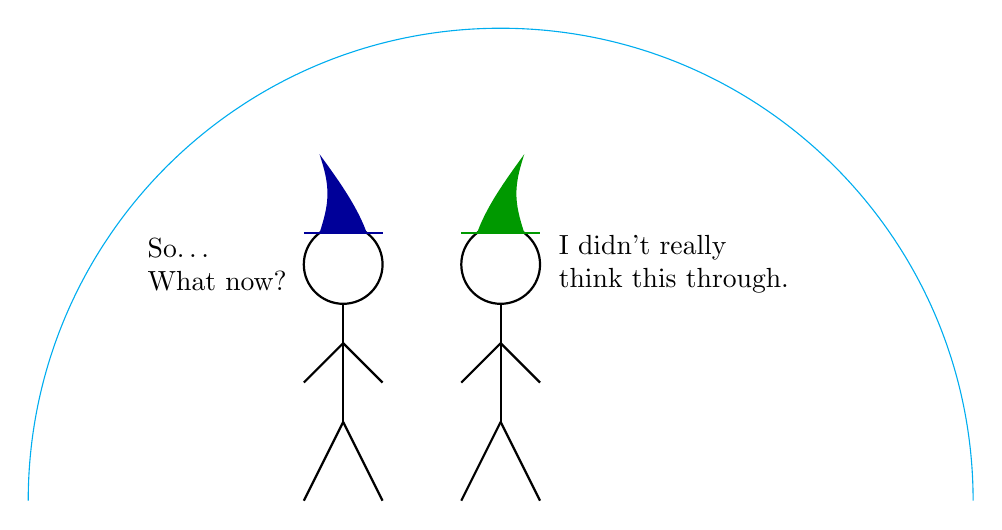
\begin{tikzpicture}
    % bubble
    \draw [cyan] (6,0) arc [start angle=0, delta angle=180, radius=6];

    { % left
      % head circle
      \draw [black,thick] (-2,3) circle [radius=0.5];
      % body stick
      \draw [black,thick] (-2,2.5) -- (-2,1);
      % arms: left, right
      \draw [black,thick] (-2,2) -- (-2.5,1.5);
      \draw [black,thick] (-2,2) -- (-1.5,1.5);
      % feet: left, right
      \draw [black,thick] (-2,1) -- (-2.5,0);
      \draw [black,thick] (-2,1) -- (-1.5,0);

      % hat
      \draw [black!40!blue,thick] (-2.5,3.4) -- (-1.5,3.4);
      %\fill [black!40!blue] plot [domain=-0.3:0.3] (-2.3,4.4) -- plot [domain=-2.3:-1.7] (\x,3.4);
      \fill [black!40!blue] plot [domain=0:1] ({-2.3+0.1*sin(180*\x)},3.4+\x) -- plot [domain=1:0] ({-2.3+0.6*cos(30+60*\x)/cos(30)},3.4+\x);

      % speech text
      \node [align=left] at (-3.6,3) {So\ldots\\What now?};
    }

    { % right
      % head circle
      \draw [black,thick] (0,3) circle [radius=0.5];
      % body stick
      \draw [black,thick] (0,2.5) -- (0,1);
      % arms: left, right
      \draw [black,thick] (0,2) -- (-0.5,1.5);
      \draw [black,thick] (0,2) -- (0.5,1.5);
      % feet: left, right
      \draw [black,thick] (0,1) -- (-0.5,0);
      \draw [black,thick] (0,1) -- (0.5,0);

      % hat
      \draw [black!40!green,thick] (-0.5,3.4) -- (0.5,3.4);
      %\fill [black!40!green] plot [domain=-0.3:0.3] (0.3,4.4) -- plot [domain=-0.3:0.3] (\x,3.4);
      \fill [black!40!green] plot [domain=0:1] ({0.3-0.1*sin(180*\x)},3.4+\x) -- plot [domain=1:0] ({0.3-0.6*cos(30+60*\x)/cos(30)},3.4+\x);

      % speech text
      \node [align=left] at (2.2,3) {I didn't really\\think this through.};
    }
  \end{tikzpicture}
\end{figure*}

An invisible barrier surrounds you and moves with you. 
The space within this barrier is impervious to most magical effects, including spells, spell-like abilities, and supernatural abilities. 
Likewise, it prevents the functioning of any magic items or spells within its confines.

An antimagic field suppresses any spell or magical effect used within, brought into, or cast into the area, but does not dispel it. 
Time spent within an antimagic field counts against the suppressed spell's duration.

Summoned creatures of any type and incorporeal undead wink out if they enter an antimagic field. 
They reappear in the same spot once the field goes away. 
Time spent winked out counts normally against the duration of the conjuration that is maintaining the creature. 
If you cast antimagic field in an area occupied by a summoned creature that has spell resistance, you must make a caster level check (1d20 + caster level) 
against the creature's spell resistance to make it wink out. 
(The effects of instantaneous conjurations are not affected by an antimagic field because the conjuration itself is no longer in effect, only its result.)

A normal creature can enter the area, as can normal missiles. Furthermore, while a magic sword does not function magically within the area, 
it is still a sword (and a masterwork sword at that). 
The spell has no effect on golems and other constructs that are imbued with magic during their creation process and are thereafter self-supporting 
(unless they have been summoned, in which case they are treated like any other summoned creatures). 
Elementals, corporeal undead, and outsiders are likewise unaffected unless summoned. 
These creatures' spell-like or supernatural abilities, however, may be temporarily nullified by the field. 
\nameref{Spell:DispelMagic} does not remove the field, though \nameref{Spell:Disjunction} might.

An antimagic field does not block line of sight or line of effect.

Two or more antimagic fields sharing any of the same space have no effect on each other. 
Certain spells, such as \nameref{Spell:WallOfForce}, \nameref{Spell:PrismaticSphere}, and \nameref{Spell:PrismaticWall} 
remain unaffected by antimagic field (see the individual spell descriptions). 
Artifacts and deities are unaffected by mortal magic such as this.

% Should a creature be larger than the area enclosed by the barrier, any part of it that lies outside the barrier is unaffected by the field. 
A creature with a space larger than a 5' square can be partially covered by an antimagic field.
If at least half of the squares the creature occupies are covered by an antimagic field, the creature acts as if it were fully enclosed within the field,
otherwise it can act unhindered.

A creature standing in a square not covered by an antimagic field can reach into the field without suffering any of its effects
(the antimagic field does not suppress magic instantaneously enough to affect those who are simply taking advantage of their reach).
For example, an Ogre wielding a magical longspear could attack a mage covered by an antimagic field from the edge of his reach, 
and still gain the benefits of the spear's magical enhancements.

\paragraph{Augment:} You can augment this spell in one or more of the following ways:
\begin{enumerate}
 \item If you spend 2 additional spell points, this spell's duration increases to 1 minute per level.
 \item For every 2 additional spell points you spend, the spell's range and radius of the area increases by 5'.
 \item If you spend 6 additional spell points, the antimagic field remains stationary at the location you cast the spell,
 rather than moving with you.
\end{enumerate}
\subsubsection{Antipoison}
\label{Spell:Antipoison}
Necromancy (Healing)
\\ \textbf{Level:} Healing 2, Paladin 2, Ranger 2
\\ \textbf{Components:} V, S
\\ \textbf{Casting Time:} 1 standard action
\\ \textbf{Range:} Touch
\\ \textbf{Target:} Creature touched
\\ \textbf{Duration:} 1 hour/level
\\ \textbf{Saving Throw:} Fortitude negates (harmless)
\\ \textbf{Spell Resistance:} Yes (harmless)
\\ \textbf{Spell Points:} 3

\emph{''You are safe. For now.``}

The subject becomes temporarily immune to poison. 
Any poison in its system or any poison to which it is exposed during the spell's duration does not affect the subject until the spell's duration has expired. 
Antipoison does not cure any damage that poison may have already done.

\paragraph{Augment:} If you spend 4 additional spell points, any poison in the subject's system as well as any poison it suffers for the spell's duration is fully neutralized, negating the need to make saving throws against the poison at the end of the spell's duration.
\subsubsection{Arachnophobia}
\label{Spell:Arachnophobia}
Enchantment (Compulsion) [Fear, Mind-Affecting]
\\ \textbf{Level:} Vermin 2
\\ \textbf{Components:} V, S
\\ \textbf{Casting Time:} 1 standard action
\\ \textbf{Range:} Close (25 ft. + 5 ft./2 levels)
\\ \textbf{Target:} One creature
\\ \textbf{Duration:} 1 round/level
\\ \textbf{Saving Throw:} Will negates
\\ \textbf{Spell Resistance:} Yes
\\ \textbf{Spell Points:} 3

\emph{''Get them off! Get them off! Don't just stand there!``} 

The subject of the spell must succeed on a will save or fall prone, believing it is covered in disgusting, lethal spiders. 
The subject can take no actions while deluded in this way (it is \emph{dazed}), but is not considered helpless.

\subsubsection{Arcane Eye}
\label{Spell:ArcaneEye}
Divination (Scrying)
\\ \textbf{Level:} Assassin 4, Sor/Wiz 4
\\ \textbf{Components:} V, S
\\ \textbf{Casting Time:} 1 standard action
\\ \textbf{Range:} Unlimited
\\ \textbf{Effect:} Magical sensor
\\ \textbf{Duration:} 1 min./level (D); see text
\\ \textbf{Saving Throw:} None
\\ \textbf{Spell Resistance:} No
\\ \textbf{Spell Points:} 7

\emph{You feel cross-eyed for a moment, before your senses readjust to incorporate the input of the sensor flying in front of you.}

You create an invisible magical sensor that sends you visual information. 
It cannot be destroyed by physical attacks, but it can be dispelled.
You can create the arcane eye at any point you can see, but it can then travel outside your line of sight without hindrance. 
An arcane eye travels at 30 feet per round (300 feet per minute) 
if viewing an area ahead as a human would (primarily looking at the floor) 
or 10 feet per round (100 feet per minute) if examining the ceiling and walls as well as the floor ahead. 
It sees exactly as you would see if you were there.

The eye can travel in any direction as long as the spell lasts. 
Solid barriers block its passage, but it can pass through a hole or space as small as 1 inch in diameter. 
The eye can't enter another plane of existence, even through a gate or similar magical portal.

You must concentrate to use an arcane eye. If you do not concentrate, the eye is inert until you again concentrate.

\paragraph{Augment:} You can augment this spell in one or more of the following ways:
\begin{enumerate}
 \item If you spend two additional spell points, you do not have to concentrate to see through the
 eye, allowing you to act unhindered while the spell is in effect.
 \item If you spend two additional spell points, the spell's duration is increased to 10 minutes per level.
\end{enumerate}

\subsubsection{Astral Projection} 
\label{Spell:AstralProjection}
Necromancy
\\ \textbf{Level:} Sor/Wiz 9, Travel 9
\\ \textbf{Components:} V, S
\\ \textbf{Casting Time:} 30 minutes
\\ \textbf{Range:} Touch
\\ \textbf{Targets:} You plus one additional willing creature touched per two caster levels
\\ \textbf{Duration:} See text
\\ \textbf{Saving Throw:} None
\\ \textbf{Spell Resistance:} Yes
\\ \textbf{Spell Points:} 17

\emph{You free your spirit from your physical body.}

This spell allows you to project an astral body onto another plane altogether.

You can bring the astral forms of other willing creatures with you, 
provided that these subjects are linked in a circle with you at the time of the casting. 
These fellow travelers are dependent upon you and must accompany you at all times. 
If something happens to you during the journey, your companions are stranded wherever you left them.

You project your astral self onto the Astral Plane, 
leaving your physical body behind on the Material Plane in a state of suspended animation. 
The spell projects an astral copy of you and all you wear or carry onto the Astral Plane
(astral copies of gear removed from the astral copy of the creature that attends it disappears, and does not reappear while the spell lasts). 
Since the Astral Plane touches upon other planes, you can travel astrally to any of these other planes as you will. 
To enter one, you leave the Astral Plane, forming a new physical body (and equipment) on the plane of existence you have chosen to enter.

While you are on the Astral Plane, your astral body is connected at all times to your physical body by a silvery cord. 
If the cord is broken, you are killed, astrally and physically, and your soul is lost on the Astral Plane. 
Raising you from the dead after your soul has been lost in this way requires a casting a \nameref{Spell:Wish} or \nameref{Spell:Miracle} 
spell prior to casting the spell that should raise you in order to retreive the soul.
%Luckily, very few things can destroy a silver cord. 
A silver cord has hardness 10, and 20 hit points. 
It can be sundered as a piece of equipment can.
A hit by a sword made of silver instantly destroys a silver cord.

When a second body is formed on a different plane, the incorporeal silvery cord remains invisibly attached to the new body. 
If the second body or the astral form is slain, 
the cord simply returns to your body where it rests on the Material Plane, thereby reviving it from its state of suspended animation. 
Although astral projections are able to function on the Astral Plane, 
their actions affect only creatures existing on the Astral Plane; a physical body must be materialized on other planes.

You and your companions may travel through the Astral Plane indefinitely. 
Your bodies simply wait behind in a state of suspended animation until you choose to return your spirits to them. 
The spell lasts until you desire to end it, or until it is terminated by some outside means, 
such as a successful \nameref{Spell:DispelMagic} spell cast upon either the physical body or the astral form, 
the breaking of the silver cord, or the destruction of your body back on the Material Plane (which kills you).

This spell can only be cast on the Material Plane.

\emph{Experience cost:} 200XP.

\subsubsection{Atonement}
\label{Spell:Atonement}
Abjuration
\\ \textbf{Level:} Blackguard 5, Chaos 5, Evil 5, Good 5, Law 5, Paladin 5
\\ \textbf{Components:} V, S
\\ \textbf{Casting Time:} 1 hour
\\ \textbf{Range:} Touch
\\ \textbf{Target:} Living creature touched
\\ \textbf{Duration:} Instantaneous
\\ \textbf{Saving Throw:} None
\\ \textbf{Spell Resistance:} Yes
\\ \textbf{Spell Points:} 9, XP

\emph{''You knelt as a sinner. Rise now as a righteous man.``}

This spell removes the burden of evil acts or misdeeds from the subject. 
The creature seeking atonement must be truly repentant and desirous of setting right its misdeeds, or the spell fails.

Some casters first assign a subject of this sort a quest (see \nameref{Spell:GeasQuest}) or similar penance to determine whether the creature is truly contrite 
before attempting to cast the atonement spell on its behalf.

Atonement may be cast for one of several purposes, depending on the version selected.
\begin{itemize}
\item \emph{Reverse Magical Alignment Change:}
If a creature has had its alignment magically changed, atonement returns its alignment to its original status.
\item \emph{Restore Power:}
A Cleric or Paladin who has lost access to its class features by violating a code of conduct may regain his abilities by seeking atonement 
from another Cleric of the same deity or a Paladin of the same order.
\item \emph{Redemption or Temptation:}
You may cast this spell upon a creature in order to offer it a chance to change its alignment to match yours. 
The prospective subject must be present for the entire casting process. Upon completion of the spell, 
the subject freely chooses whether it retains its original alignment or acquiesces to your offer and changes to your alignment. 
No duress, compulsion, or magical influence can force the subject to take advantage of the opportunity offered if it is unwilling to abandon its old alignment. 
This use of the spell does not work on outsiders or any creature incapable of changing its alignment naturally.

In the case of Clerics and Paladins that have switched to an inappropriate alignment, this use of the spell may be required in order to restore their abilities.
\end{itemize}

Though the spell description refers to evil acts, 
atonement can also be used on any creature that has performed acts against its alignment, whether those acts are evil, good, chaotic, or lawful.

\emph{Note:} Normally, changing alignment is up to the player. 
This use of atonement simply offers a believable way for a character to change his or her alignment drastically, suddenly, and definitively.
 
\emph{Experience cost:} 500 XP
\subsubsection{Augury}
\label{Spell:Augury}
Divination
\\ \textbf{Level:} Cleric 2
\\ \textbf{Components:} V, S
\\ \textbf{Casting Time:} 1 minute
\\ \textbf{Range:} Personal
\\ \textbf{Target:} You
\\ \textbf{Duration:} Instantaneous
\\ \textbf{Spell Points:} 3

\emph{''Oh, grand poobah, grant me this answer...``}

An augury can tell you whether a particular action will bring good or bad results for you in the immediate future.

The base chance for receiving a meaningful reply is 70\% + 1\% per caster level, to a maximum of 90\%; this roll is made secretly. 
A question may be so straightforward that a successful result is automatic, or so vague as to have no chance of success. 
If the augury succeeds, you get one of four results:

\begin{itemize}
 \item Weal (if the action will probably bring good results).
 \item Woe (for bad results).
 \item Weal and woe (for both).
 \item Nothing (for actions that don't have especially good or bad results).
\end{itemize}
If the spell fails, you get the ''nothing`` result. A cleric who gets the ''nothing`` result has no way to tell whether it was the consequence of a failed or successful augury.

The augury can see into the future only about half an hour, so anything that might happen after that does not affect the result. 
Thus, the result might not take into account the long-term consequences of a contemplated action. 
All auguries cast by the same person about the same topic use the same dice result as the first casting.

\paragraph{Augment:} If you spend 4 additional spell points, the spell can provide you with a useful piece of advice in reply to a question concerning a specific goal, event, or activity that is to occur within one week, rather than just one of the four results shown above. 
The advice can be as simple as a short phrase, or it might take the form of a cryptic rhyme or omen. 
If your party doesn't act on the information, the conditions may change so that the information is no longer useful. 
The base chance for a correct divination of this kind is still 70\% + 1\% per caster level, to a maximum of 90\%. 
However, if the dice roll fails, you know the spell failed, unless specific magic yielding false information is at work.
Multiple divinations about the same topic by the same caster still use the same dice result as the first Augury spell and yield the same answer each time.
\subsubsection{Aura of Fire}
\label{Spell:AuraOfFire}
Evocation [Fire]
\\ \textbf{Level:} Fire 4, Sor/Wiz 4, Sun 4
\\ \textbf{Components:} V, S
\\ \textbf{Casting Time:} 1 standard action
\\ \textbf{Range:} Personal
\\ \textbf{Target:} You
\\ \textbf{Duration:} 1 round/level (D)
\\ \textbf{Spell Resistance:} See text
\\ \textbf{Spell points:} 7

\emph{Fires dance along your skin, but they do not burn you.}

This spell wreathes you in flames which cause damage to nearby creatures, more to those that attack you in melee.
The flames also protect you from cold-based attacks.

At the time of casting, and at the start of each of your turns for the spell's duration, each enemy creature within
30' takes 3d6 points of fire damage.
No saving throw is allowed against this damage, but Spell Resistance applies.

In addition, a creature striking you with its body or a handheld weapon takes this damage every time it attacks,
regardless of whether the attack hits.
Creatures wielding weapons with exceptional reach are not subject to this additional damage if they attack you.

When casting this spell, you appear to immolate yourself, but the flames are thin and wispy, 
giving off light equal to only half the illumination of a normal torch (10 feet). 

You take only half damage from cold-based attacks. 
If such an attack allows a Reflex save for half damage, you take no damage on a successful save.

\paragraph{Augment:} For every 2 additional spell points you spend, this spell's damage increases by 1d6.

\paragraph{Special:} You can choose to create an Aura of Cold rather than an Aura of Flame. This changes the damage
dealt by the spell to cold damage, the spell's descriptor to [cold], and the protection from attacks to one
against fire-based attacks.
\subsubsection{Awaken}
\label{Spell:Awaken}
Transmutation
\\ \textbf{Level:} Animal 5, Plant 5, Ranger 5
\\ \textbf{Components:} V, S
\\ \textbf{Casting Time:} 24 hours
\\ \textbf{Range:} Touch
\\ \textbf{Target:} Animal or tree touched
\\ \textbf{Duration:} Instantaneous
\\ \textbf{Saving Throw:} Will negates
\\ \textbf{Spell Resistance:} Yes
\\ \textbf{Spell Points:} 9

\emph{The creature opens its eyes, a new intelligence in its eyes.}

You awaken a tree or animal to humanlike sentience. %To succeed, you must make a Will save (DC 10 + the animal's current HD, or the HD the tree will have once awakened).
The awakened animal or tree is friendly toward you. You have no special empathy or connection with a creature you awaken, although it serves you in specific tasks or endeavors if you communicate your desires to it.

An awakened tree has characteristics as if it were an animated object, except that it gains the plant type and its Intelligence, Wisdom, and Charisma scores are each 3d6. 
An awakened plant gains the ability to move its limbs, roots, vines, creepers, and so forth, and it has senses similar to a human's.

An awakened animal gets 3d6 Intelligence and +1d3 Charisma. Its type becomes magical beast (augmented animal). 
An awakened animal can't serve as an animal companion, familiar, or special mount.

An awakened tree or animal can speak one language that you know, plus one additional language that you know per point of its Intelligence bonus (if any).

A creature who wishes to resume being a normal specimen of its kind can do so by employing a \nameref{Spell:LimitedWish}, \nameref{Spell:Miracle} or \nameref{Spell:Wish} spell, although it is unusual for an awakened creature to desire this. An awakened creature cannot be returned to normal against its will.

Logically, once a creature has been awakened, it cannot be awakened again unless it is first returned to normal.

\emph{Experience Cost:} 250 XP.

\emph{Special:} This spell cannot be enhanced by the \nameref{Feat:EmpowerSpell} or \nameref{Feat:MaximizeSpell} feats.
\subsubsection{Awaken Nature's Wrath}
\label{Spell:AwakenNaturesWrath}
Transmutation
\\ \textbf{Level:} Plant 9
\\ \textbf{Components:} V, S
\\ \textbf{Casting Time:} 1 hour
\\ \textbf{Range:} 1 mile
\\ \textbf{Area:} 1-mile radius spread, centered on you
\\ \textbf{Duration:} 1 day/level
\\ \textbf{Saving Throw:} None
\\ \textbf{Spell Resistance:} No
\\ \textbf{Spell Points:} 17

\emph{You awaken nature's most ancient forces, causing it to roil up and defend itself against intruders.}

One minute after entering the spell's area, any aberration, construct, dragon, giant, humanoid, monstrous humanoid, ooze, outsider or undead creature takes 10d6 points of damage as the surrounding terrain and flora animate and viciously attack. This damage is repeated once per round thereafter, until the creature leaves the area. 

Aside from attacking, the environment is not significantly changed. Retaliation against terrain and objects that attack you is possible, but does not prevent further damage.

When you cast the spell, you gain knowledge of a password, unique to that casting of the spell. You, or any creature you share the password with, can speak this word after entering the area but before the attacks begin in order to negate the damage (for the creature who spoke it only).

This spell only affects natural terrain, not places where settlements (such as villages and dungeons) have replaced the natural setting. If any part of the area of the spell overlaps a place of settlement, that part is unaffected.

Any creature unaware of the spell when entering the area is entitled to a DC 20 Wisdom check to notice that the area is terribly dangerous.

\emph{Special:} This spell cannot be dispelled via normal means, nor can it be dismissed. Only a properly worded \nameref{Spell:Miracle} or \nameref{Spell:Wish} spell can calm the area before the spell's duration expires.

\paragraph{Augment:} For every additional spell point you spend, this spell's range and area increase by one mile each.
\subsection{'B' Spells}
\subsubsection{Baleful Polymorph}
\label{Spell:BalefulPolymorph}
Transmutation
\\ \textbf{Level:} Animal 5, Ranger 5, Sor/Wiz 5
\\ \textbf{Components:} V, S
\\ \textbf{Casting Time:} 1 standard action
\\ \textbf{Range:} Close (25 ft. + 5 ft./2 levels)
\\ \textbf{Target:} One creature
\\ \textbf{Duration:} Permanent
\\ \textbf{Saving Throw:} Fortitude negates, Will partial; see text
\\ \textbf{Spell Resistance:} Yes
\\ \textbf{Spell Points:} 9

\emph{''It will take more than a kiss to save you now! ``}

You change the subject into a Small or smaller animal of no more than 1 HD (such as a dog, lizard, monkey, or toad). 
The subject takes on all the statistics and special abilities of an average member of the new form in place of its own except as follows:

\begin{itemize}
 \item The target retains its own alignment (and personality, within the limits of the new form's ability scores).
 \item The target retains its own hit points.
 \item The target is treated as having its normal Hit Dice for purpose of adjudicating effects based on HD, such as the \nameref{Spell:Sleep} spell, though it uses the new form's base attack bonus, base save bonuses, and all other statistics derived from Hit Dice.
 \item The target also retains the ability to understand (but not to speak) the languages it understood in its original form. It can write in the languages it understands, but only the form is capable of writing in some manner (such as drawing in the dirt with a paw).
\end{itemize}
With those exceptions, the target's normal game statistics are replaced by those of the new form. The target loses all the special abilities it has in its normal form, including its class features.

All items worn or carried by the subject fall to the ground at its feet, even if they could be worn or carried by the new form.

If the new form would prove fatal to the creature (for example, if you polymorphed a landbound target into a fish, or an airborne target into a toad), the subject gets a +4 bonus on the save.

If the subject remains in the new form for 24 consecutive hours, it must attempt a Will save. 
If this save fails, it loses its ability to understand language, as well as all other memories of its previous form, and its Hit Dice and hit points change to match an average creature of its new form. These abilities and statistics return to normal if the effect is later ended.

Incorporeal or gaseous creatures are immune to baleful polymorph, and a creature with the shapechanger subtype (such as a lycanthrope or a doppelganger) can revert to its natural form as a standard action (which ends the spell's effect).

\paragraph{Augment:} If you spend 4 additional spell points, the Will save to avoid memory loss and other drawbacks associated with it must be made immediately following the fortitude save, 
rather than 24 hours later.

\emph{Note:} This is not a polymorph subschool spell.


\paragraph{Augment:} The spell gains an augment in addition to the ones inherited from Raise Dead:
\begin{itemize}
 \item If you spend 4 additional spell points, the creature to be returned from the dead can be unwilling.
An unwilling creature is allowed a will save with a +5 bonus 
(but no bonuses for items, active spells, or other effects 
that may be affecting its corpse at the time of death or the attempted resurrection)
to negate the spell.

A subject that successfully saves cannot be the victim of a forced resurrection for a year and a day, 
or until it is raised (voluntarily) and killed again, whichever happens sooner.
\end{itemize}

\emph{Experience cost:} 200XP.
\subsubsection{Bane}
\label{Spell:Bane}
Enchantment (Compulsion) [\nameref{sec:Curses}, Evil, Fear, Mind-Affecting]
\\ \textbf{Level:} Blackguard 1
\\ \textbf{Components:} V, S
\\ \textbf{Casting Time:} 1 standard action
\\ \textbf{Range:} 40 ft.
\\ \textbf{Area:} All enemies within a 40-ft. radius burst centered on you
\\ \textbf{Duration:} 1 round/level
\\ \textbf{Saving Throw:} None
\\ \textbf{Spell Resistance:} Yes
\\ \textbf{Spell Points:} 1

\emph{You fill your enemies with fear and doubt.}

Each affected creature takes a -1 penalty on attack rolls and a -1 penalty on saving throws against fear effects.

\paragraph{Augment:} You can Augment the spell in one or more of the following ways:
\begin{enumerate}
 \item If you spend 2 additional spell points, the penalty applies to all saving throws (not just saves vs. fear), weapon damage rolls, and skill checks, in addition to attack rolls.
 \item If you spend 2 additional spell points, this spell affects allies as well as enemies within the area.
 Allies affected by the spell receive a luck bonus on the appropriate rolls equal to the penalty inflicted on your enemies.
 \item For every 4 additional power points you spend, the penalty to the appropriate rolls increases by 1.
 \item If you spend 1 additional spell point, this spell's duration increases to one minute per level.
\end{enumerate}

\subsubsection{Barkskin}
\label{Spell:Barkskin}
Transmutation
\\ \textbf{Level:} Plant 2, Ranger 2
\\ \textbf{Components:} V, S
\\ \textbf{Casting Time:} 1 standard action
\\ \textbf{Range:} Touch
\\ \textbf{Target:} Living creature touched
\\ \textbf{Duration:} 10 min./level
\\ \textbf{Saving Throw:} None
\\ \textbf{Spell Resistance:} Yes (harmless)
\\ \textbf{Spell Points:} 3

\emph{The creature's skin toughens.}

\begin{figure*}
  \caption{Druid explains the virtue of his Barkskin spell to a Wizard buddy.}
  \centering
    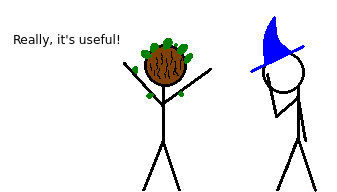
\includegraphics{Pics/Barkskin.png}
\end{figure*}

Barkskin grants a +2 enhancement bonus to the creature's existing natural armor bonus.

The enhancement bonus provided by barkskin stacks with the target's natural armor bonus, but not with other enhancement bonuses to natural armor. A creature without natural armor has an effective natural armor bonus of +0.

\paragraph{Augment:} For every 2 additional spell points you spend, the enhancement bonus to the creature's natural armor increases by 1.
\subsubsection{Bestow Curse}
\label{Spell:BestowCurse}
Necromancy [\nameref{sec:Curses}]
\\ \textbf{Level:} Blackguard 4, Evil 3, Luck 3, Sor/Wiz 4
\\ \textbf{Components:} V, S
\\ \textbf{Casting Time:} 1 standard action
\\ \textbf{Range:} Touch
\\ \textbf{Target:} Creature touched
\\ \textbf{Duration:} Permanent (D)
\\ \textbf{Saving Throw:} Will negates
\\ \textbf{Spell Resistance:} Yes
\\ \textbf{Spell Points:} Blackguard 7, Evil 5, Luck 5, Sor/Wiz 7

\emph{''A pox upon you! A POX!``}

You place a curse on the subject. Choose one of the following three effects.
\begin{itemize}
 \item -6 decrease to an ability score (minimum 1).
 \item -4 penalty on attack rolls, saves, ability checks, and skill checks.
 \item Each turn, the target has a 50\% chance to act normally; otherwise, it takes no action.
\end{itemize}
The GM may add additional, more unique options to this spell, 
but they should be no more powerful than those described above (particularly when it comes to in-combat applications).

The curse bestowed by this spell cannot be dispelled, but see \nameref{sec:RemovingACurse}.

\paragraph{Augment:} If you spend an additional 6 spell points, you can select from a different menu of options:
\begin{enumerate}
 \item One of the subject's ability scores are reduced to 1.
 \item -8 penalty on attack rolls, saves, ability checks, and skill checks.
 \item Each turn, the target has a 25\% chance to act normally; otherwise, it takes no action.
\end{enumerate}
\subsubsection{Binding}
\label{Spell:Binding}
Enchantment (Compulsion) [Mind-Affecting]
\\ \textbf{Level:} Sor/Wiz 8 
\\ \textbf{Components:} V, S 
\\ \textbf{Casting Time:} One minute 
\\ \textbf{Range:} Close (25 ft. + 5 ft./2 levels)
\\ \textbf{Target:} One living creature 
\\ \textbf{Duration:} See text (D)
\\ \textbf{Saving Throw:} Will negates; see text
\\ \textbf{Spell Resistance:} Yes
\\ \textbf{Spell Points:} 15, XP

\emph{''And you shall remain this way until the king's castle is raised above the clouds!``}

A binding spell creates a magical restraint to hold a creature. 
The target gets an initial saving throw only if its Hit Dice equal at least one-half your caster level.

% You may have as many as six assistants help you with the spell. 
% For each assistant who casts suggestion, your caster level for this casting of binding increases by 1. 
% For each assistant who casts dominate animal, dominate person, or dominate monster, 
% your caster level for this casting of binding increases by a number equal to one-third of that assistant's level, 
% provided that the spell's target is appropriate for a binding spell. 
% Since the assistants' spells are cast simply to improve your caster level for the purpose of the binding spell, 
% saving throws and spell resistance against the assistants' spells are irrelevant. 
% Your caster level determines whether the target gets an initial Will saving throw and how long the binding lasts. 
All binding spells are dismissible.

Regardless of the version of binding you cast, 
you can specify triggering conditions that end the spell and release the creature whenever they occur. 
These triggers can be as simple or elaborate as you desire, but the condition must be reasonable and have a likelihood of coming to pass. 
The conditions can be based on a creature's name, identity, or alignment but otherwise must be based on observable actions or qualities. 
Intangibles such as level, class, Hit Dice, or hit points don't qualify. 
Once the spell is cast, its triggering conditions cannot be changed. 
Setting a release condition increases the save DC (assuming a saving throw is allowed) by 2.

If you are casting any of the first three versions of binding (those with limited durations), 
you may cast additional binding spells to prolong the effect, since the durations overlap. 
If you do so, the target gets a saving throw at the end of the first spell's duration, 
even if your caster level was high enough to disallow an initial saving throw. 
If the creature succeeds on this save, all the binding spells it has received are broken.

The binding spell has six versions. Choose one of the following versions when you cast the spell.
\begin{itemize}
 \item \emph{Chaining:}
The subject is confined by restraints that generate an \nameref{Spell:TelepathicBeacon} spell (the repulsion version) affecting all creatures who approach the subject, except you. 
The duration is one year per caster level. 
The subject of this form of binding is confined to the spot it occupied when it received the spell.
\item \emph{Slumber:}
This version causes the subject to become comatose for as long as one year per caster level. 
The subject does not need to eat or drink while slumbering, nor does it age. 
This form of binding is more difficult to cast than chaining, making it slightly easier to resist. Reduce the spell's save DC by 1.
 \item \emph{Bound Slumber:}
This combination of chaining and slumber lasts for as long as one month per caster level. Reduce the save DC by 2.
 \item \emph{Hedged Prison:}
The subject is transported to or otherwise brought within a confined area from which it cannot wander by any means. 
The effect is permanent. Reduce the save DC by 3.
 \item \emph{Metamorphosis:}
The subject assumes gaseous form, except for its head or face. 
It is held harmless in a jar or other container, which may be transparent if you so choose. 
The creature remains aware of its surroundings and can speak, but it cannot leave the container, attack, or use any of its powers or abilities. 
The binding is permanent. 
The subject does not need to breathe, eat, or drink while metamorphosed, nor does it age. Reduce the save DC by 4.
 \item \emph{Minimus Containment:}
The subject is shrunk to a height of 1 inch or even less and held within some gem, jar, or similar object. 
The binding is permanent. The subject does not need to breathe, eat, or drink while contained, nor does it age. Reduce the save DC by 4.
\end{itemize}
You can't dispel a binding spell with \nameref{Spell:DispelMagic} or a similar effect, 
though an \nameref{Spell:AntimagicField} field or \nameref{Spell:Disjunction} affects it normally. 
A bound extraplanar creature cannot be sent back to its home plane due to dismissal, banishment, or a similar effect.

You must have specially made props suited to the specific type of binding at hand when you cast the spell.

\emph{Experience cost:} 100 XP + 100 XP per HD of the creature to be bound.
\subsubsection{Blackfire}
\label{Spell:Blackfire}
Evocation
\\ \textbf{Level:} Assassin 1, Blackguard 1
\\ \textbf{Components:} V, S
\\ \textbf{Casting Time:} 1 standard action
\\ \textbf{Range:} Medium (100 ft. + 10 ft./level)
\\ \textbf{Targets:} Up to one source of light/level
\\ \textbf{Duration:} 1 round/level (D)
\\ \textbf{Saving Throw:} Will negates (object); see text
\\ \textbf{Spell Resistance:} Yes (object); see text
\\ \textbf{Spell Points:} 1

\emph{The fires turn black, but continue to shed their light... at least as far as you are concerned.}

The light emitted by the targeted light sources changes in nature.
For you, the light sources shed light as brightly as ever before, but as far as anyone else is concerned, their light has completely vanished.

Secondary characteristics of the light sources remain unaffected, fires still are still hot, glowing magic weapons are still magic weapons, and so forth, but they no longer illuminate their surroundings for anyone but you.

You can target covered fires, such as those of lanterns. If a targeted source of fire sets another object on fire, the new object sheds light normally.

\paragraph{Augment:} You can augment this spell in one or both of the following ways:
\begin{enumerate}
 \item If you spend 2 additional spell points, this spell's duration increases to 10 minutes per level.
 \item For every 2 additional spell points you spend, you may designate one creature that shares your ability to see by the affected light sources.
\end{enumerate}
\subsubsection{Black Tentacles}
\label{Spell:BlackTentacles}
Conjuration (Creation)
\\ \textbf{Level:} Conjurer 4
\\ \textbf{Components:} V, S
\\ \textbf{Casting Time:} 1 standard action
\\ \textbf{Range:} Medium (100 ft. + 10 ft./level)
\\ \textbf{Area:} 20-ft.-radius spread
\\ \textbf{Duration:} 1 round/level (D)
\\ \textbf{Saving Throw:} None
\\ \textbf{Spell Resistance:} No
\\ \textbf{Spell Points:} 7

\emph{''The horror... the horror!``}

This spell conjures a field of rubbery black tentacles, each 10 feet long. 
These waving members seem to spring forth from the earth, floor, or whatever surface is underfoot (including water). 
They grasp and entwine around creatures that enter the area, holding them fast and crushing them with great strength.

Every creature within the area of the spell must make a grapple check, opposed by the grapple check of the tentacles. 
Treat the tentacles attacking a particular target as a Large creature with a base attack bonus equal to your caster level and a Strength score of 19. 
Thus, its grapple check modifier is equal to your caster level +8. 
The tentacles are immune to all types of damage.

Once the tentacles grapple an opponent, they may make a grapple check each round on your turn to deal 1d6+4 points of bludgeoning damage. 
The tentacles continue to crush the opponent until the spell ends or the opponent escapes.

Any creature that enters the area of the spell is immediately attacked by the tentacles. 
Even creatures who aren't grappling with the tentacles may move through the area at only half normal speed.

\paragraph{Augment:} 
% You can augment this spell in one or both of the following ways:
% \begin{enumerate}
%  \item 
If you spend 2 additional spell points, the tentacles grow
\href{http://www.giantitp.com/comics/oots0020.html}{wicked spikes}. 
The damage dealt by the tentacles changes to piercing and slashing damage, and increases to 1d6 + your caster level.
%  \item If you spend 4 additional spell points, the tentacles' length increases to 15 feet, and they count as a huge
%  creature. This increases their grapple check modifier to your caster level +12.
% \end{enumerate}

\subsubsection{Blade Barrier}
\label{Spell:BladeBarrier}
Evocation [Force]
\\ \textbf{Level:} Good 6, War 6
\\ \textbf{Components:} V, S
\\ \textbf{Casting Time:} 1 standard action
\\ \textbf{Range:} Medium (100 ft. + 10 ft./level)
\\ \textbf{Effect:} Wall of whirling blades up to 20 ft. long/level, or a ringed wall of whirling blades with a radius of up to 5 ft. per two levels; either form 20 ft. high
\\ \textbf{Duration:} 1 min./level (D)
\\ \textbf{Saving Throw:} None or Reflex negates; see text
\\ \textbf{Spell Resistance:} Yes
\\ \textbf{Spell Points:} 11

\emph{An immobile, vertical curtain of whirling blades shaped of pure force springs into existence.}

Any creature passing through the wall you conjure takes 11d6 points of force damage, with no saving throw.
If you evoke the barrier so that it appears where creatures are, 
each creature takes damage as if passing through the wall, but each such creature can avoid the wall
(ending up on the side of its choice) and thus take no damage by making a successful Reflex save.
A blade barrier provides cover (+4 bonus to AC, +2 bonus on Reflex saves) against attacks made through it.

\paragraph{Augment:} Every additional spell point spent on this spell increases its damage by one die (d6).

\subsubsection{Bless}
\label{Spell:Bless}
Enchantment (Compulsion) [Good, Mind-Affecting]
\\ \textbf{Level:} Good 1, Luck 1, Paladin 1
\\ \textbf{Components:} V, S
\\ \textbf{Casting Time:} 1 standard action
\\ \textbf{Range:} 40 ft.
\\ \textbf{Area:} All allies within a 40-ft. radius burst centered on you
\\ \textbf{Duration:} 1 round/level
\\ \textbf{Saving Throw:} None
\\ \textbf{Spell Resistance:} Yes
\\ \textbf{Spell Points:} 1

\emph{You bring special favor upon yourself and your allies while bringing disfavor to your enemies.}

You and your each of your allies gain a +1 luck bonus on attack rolls and saves vs. fear.

\paragraph{Augment:} You can Augment the spell in one or more of the following ways:
\begin{enumerate}
 \item If you spend 2 additional spell points, the luck bonus applies to all saving throws (not just saves vs. fear),
 weapon damage rolls, and skill checks, in addition to attack rolls.
 \item If you spend 2 additional spell points, this spell affects enemies as well as allies within the area.
 Enemies affected by the spell take a penalty on the appropriate rolls equal to the luck bonus provided to your allies.
 \item For every 6 additional power points you spend, the luck bonus gained on the appropriate rolls increases by 1.
 \item If you spend 1 additional spell point, this spell's duration increases to one minute per level.
\end{enumerate}
\subsubsection{Bless Weapon}
\label{Spell:BlessWeapon}
Transmutation
\\ \textbf{Level:} Paladin 1
\\ \textbf{Components:} V, S
\\ \textbf{Casting Time:} 1 standard action
\\ \textbf{Range:} Touch
\\ \textbf{Target:} Weapon touched
\\ \textbf{Duration:} 1 min./level
\\ \textbf{Saving Throw:} None
\\ \textbf{Spell Resistance:} No
\\ \textbf{Spell Points:} 1

\emph{Your weapon strikes true against evil foes.}

The transmuted weapon is treated as being magical for the purpose of bypassing the damage reduction of evil creatures or striking evil incorporeal creatures (though the spell doesn't grant an actual enhancement bonus). 
The weapon also becomes good, which means it can bypass the damage reduction of certain creatures. 
(This effect overrides and suppresses any other alignment the weapon might have.) 
Individual arrows or bolts can be transmuted, but affected projectile weapons (such as bows) don't confer the benefit to the projectiles they shoot.

In addition, all critical hit rolls against evil foes are automatically successful, so every threat is a critical hit. 
This last effect does not apply to any weapon that already has a magical effect related to critical hits, such as a keen weapon or a vorpal sword.
\subsubsection{Blight}
\label{Spell:Blight}
Necromancy [Death, Evil]
\\ \textbf{Level:} Death 4, Sor/Wiz 5
\\ \textbf{Range:} Touch
\\ \textbf{Target:} Plant creature touched, or plant touched; see text
\\ \textbf{Spell Points:} Death 7, Sor/Wiz 9

\emph{The plant withers and dies.}

This spell functions like the \nameref{Spell:DeathKnell} spell (including Augmentation options), 
except as outlined below.

Rather than targeting a creature with -1 or fewer hit points, it targets a plant creature with any number of HP remaining.

Plants that are not creatures (most are not) can still be targeted and killed by this spell,
but they provide you with no bonuses (just like killing creatures that do not have a full HD).
Such a mundane plant receives no saving throw against this spell, it simply withers and dies,
regardless of health and size.
\subsubsection{Blindness}
\label{Spell:Blindness}
Necromancy
\\ \textbf{Level:} Blackguard 2, Evil 2, Sor/Wiz 2
\\ \textbf{Components:} V
\\ \textbf{Casting Time:} 1 standard action
\\ \textbf{Range:} Medium (100 ft. + 10 ft./level)
\\ \textbf{Target:} One living creature
\\ \textbf{Duration:} Permanent (D)
\\ \textbf{Saving Throw:} Fortitude negates
\\ \textbf{Spell Resistance:} Yes
\\ \textbf{Spell Points:} 3

\emph{''My eyes! MY EYES!``}

You call upon the powers of unlife to render one of the subject's primary senses useless.
The subject becomes \emph{blind} or \emph{deaf}, or loses one special sense it may have (such as scent, blindsight, blindsense, or tremorsense). 

The name of the spell stems from its most common usage, as most humanoids rely on their sight more than any other sense.

\subsubsection{Blink}
\label{Spell:Blink}
Conjuration (Teleportation)
\\ \textbf{Level:} Bard 3, Sor/Wiz 3
\\ \textbf{Components:} V, S
\\ \textbf{Casting Time:} 1 standard action
\\ \textbf{Range:} Touch
\\ \textbf{Target:} Creature touched
\\ \textbf{Duration:} 1 round/level (D)
\\ \textbf{Spell Points:} 5

\emph{The creature vanishes and reappears at a maddening rate.}

The subject ``blinks`` back and forth between the Material Plane and the Ethereal Plane, spending
roughly half his time on the Material Plane and half on the Ethereal Plane. 
He looks as though he's winking in and out of reality very quickly and at random
(the blinking can be controlled by neither the caster nor the subject).

Blinking has several effects on an opponent's chance to hit, as follows\footnote{
Blink effectively grants two ''different'' miss chances, although it may not be immediately obvious
(one for being simply not there half the time, the other half for not being visible all the time.
This means the spell has complicated interactions with other spells that grant similar benefits. 
Those who intend to use this spell in conjunction with others may want to spend time reading the spell descriptions thoroughly.
% For example:
% \begin{itemize}
%  \item Blur + Blink: The miss chance granted by \nameref{Spell:Blur}
%  overlaps with the ``not visible'' (concealment) 
%  aspect of Blink, combined they only grant a 20\% miss chance, 
%  or a 50\% miss chance if the Blur spell is Augmented. STUFFSTUFFSTUFF
%  \item Invisibility + Blink: The miss chance granted by \nameref{Spell:Invisibility}
%  overlaps with the ``not visible'' (concealment) 
%  aspect of Blink, combined they only grant a 50\% miss chance. STUFFSTUFFSTUFF
% \end{itemize}
}:

\begin{itemize}
 \item Physical attacks against the subject have a 50\% miss chance. 
 The Blind-Fight feat doesn't help opponents, since he is ethereal and not merely invisible.
 \item If the attacker is capable of striking ethereal creatures, but not \emph{seeing}
 ethereal creatures, the miss chance is only 20\% (for limited concealment).
 The miss chance is less than that offered by true invisibility, because the subject of the spell
 is perfectly visible half the time.
 \item If the attacker can see ethereal creatures, the miss chance is also only 20\%.
 This is because even though the attacker can't hit the subject while he is ethereal, 
 attacks can be timed to mostly hit while the subject is on the material plane.
 \item For an attacker that can both see and strike ethereal creatures, there is no miss chance.
\end{itemize}  
Likewise, your own attacks have a 20\% miss chance, 
since you sometimes go ethereal just as you are about to strike.

Any individually targeted spell has a 50\% chance to fail against you while you're blinking unless 
your attacker can target invisible, ethereal creatures. 
Your own spells have a 20\% chance to activate just as you go ethereal, 
in which case they typically do not affect the Material Plane.

While blinking, you take only half damage from area attacks 
(but full damage from those that extend onto the Ethereal Plane). 
You strike as an invisible creature (with a +2 bonus on attack rolls), 
denying your target any Dexterity bonus to AC.

You take only half damage from falling, since you fall only while you are material.

While blinking, you can step through (but not see through) solid objects. 
For each 5 feet of solid material you walk through, 
there is a 50\% chance that you become material. 
If this occurs, you are shunted off to the nearest open space and take 1d6 points of damage per 5 feet so traveled. 
You can move at only three-quarters speed 
(because movement on the Ethereal Plane is at half speed, 
and you spend about half your time there and half your time material.)

Since you spend about half your time on the Ethereal Plane, 
you can see and even attack ethereal creatures. 
You interact with ethereal creatures roughly the same way you interact with material ones.

An ethereal creature is invisible, incorporeal, 
and capable of moving in any direction, even up or down. 
As an incorporeal creature, you can move through solid objects, including living creatures.

An ethereal creature can see and hear the Material Plane, 
but everything looks gray and insubstantial. 
Sight and hearing on the Material Plane are limited to 60 feet.

Force effects and abjurations affect you normally. 
Their effects extend onto the Ethereal Plane from the Material Plane, but not vice versa. 
An ethereal creature can't attack material creatures, 
and spells you cast while ethereal affect only other ethereal things. 
Certain material creatures or objects have attacks or effects that work on the Ethereal Plane. 
Treat other ethereal creatures and objects as material.

\paragraph{Augment:} If you spend 4 additional spell points, the subject can perfectly predict its own blinking,
although it still cannot control it. This negates the 20\% effective miss chance the subject suffers on attacks, as
well as the chance of its spells accidentally going off on the ethereal plane.

\subsubsection{Blur}
\label{Spell:Blur}
Illusion (Glamer)
\\ \textbf{Level:} Sor/Wiz 2
\\ \textbf{Components:} V
\\ \textbf{Casting Time:} 1 standard action
\\ \textbf{Range:} Touch
\\ \textbf{Target:} Creature touched
\\ \textbf{Duration:} 1 round./level (D)
\\ \textbf{Saving Throw:} Will negates (harmless)
\\ \textbf{Spell Resistance:} Yes (harmless)
\\ \textbf{Spell Points:} 3

\emph{The subject's outline appears blurred, shifting and wavering.}

The glamer grants the subject concealment (20\% miss chance).

A \nameref{Spell:SeeInvisibility} spell does not counteract the blur effect, but a \nameref{Spell:TrueSeeing} spell does.

\paragraph{Augment:} You can augment this spell in one or both of the following ways:
\begin{enumerate}
 \item If you spend 4 additional spell points, the creature benefits from a 50\% miss chance as if it had total concealment. 
However, unlike actual total concealment, this augment does not prevent enemies from targeting the creature normally.
 \item If you spend 2 additional spell points, the spell's duration increases to one minute per level.
\end{enumerate}
\subsubsection{Body of Light}
\label{Spell:BodyOfLight}
Transmutation (Polymorph) [Light]
\\ \textbf{Level:} Paladin 4, Sun 5
\\ \textbf{Components:} V,S
\\ \textbf{Casting Time:} 1 standard action
\\ \textbf{Range:} Touch
\\ \textbf{Target:} Willing living creature touched
\\ \textbf{Duration:} 1 min./level (D)
\\ \textbf{Saving Throw:} None
\\ \textbf{Spell Resistance:} No
\\ \textbf{Spell Points:} Paladin 7, Sun 9

\emph{The creature's skin glows with an intense, pure light, as if constructed of it.}

The creature's skin and flesh is changed into pure light, granting it immunity to poison, sleep effects, paralysis, stunning, critical hits, and flanking.

In addition, the creature's skin sheds light as bright as full daylight in a 60-foot radius, and dim light for an additional 60 feet beyond that. 

If an area of magical light and an area of magical darkness overlap, 
the spell on which more spell points were spent prevails.
If an equal number of spell points were spent on both spells, ambient light conditions remain.

\paragraph{Augment:} If you spend 4 additional spell points, the creature is able to retain more of itself throughout the transformation.
The creature retains all its class features when polymorphed (notably, allowing spellcasting).
This is an exception to the general rules of Polymorph subschool spells.

\subsubsection{Burn}
\label{Spell:Burn}
Evocation [Fire]
\\ \textbf{Level:} Evoker 1
\\ \textbf{Components:} V, S
\\ \textbf{Casting Time:} 1 standard action
\\ \textbf{Range:} Close (25 ft. + 5 ft./2 levels)
\\ \textbf{Target:} One creature; see text
\\ \textbf{Duration:} 3 rounds
\\ \textbf{Saving Throw:} None, Reflex negates; See text
\\ \textbf{Spell Resistance:} Yes
\\ \textbf{Spell Points:} 1

\emph{``Do you remember the time when you said I was a nerd for going to Wizarding school? NOW BURN FOR IT!''}

A creature that takes fire damage while this spell is in effect magically catches on fire.
One round after catching on fire, and once per round thereafter, the spell deals additional fire damage equal to one-half the fire damage that set it on fire in the first place.
If a creature takes fire damage multiple times while the spell lasts, use one-half of the largest damage value.

The fire can be put out by any normal means, such as rolling on the ground (Reflex save DC equal to the spell's normal DC) and jumping into water.

\paragraph{Augment:} For every additional spell point you spend, this spell lasts for an additional round.
\subsection{'C' Spells}
\subsubsection{Call Lightning}
\label{Spell:CallLightning}
Evocation [Electricity]
\\ \textbf{Level:} Air 3, Destruction 3
\\ \textbf{Components:} V, S
\\ \textbf{Casting Time:} 1 standard action
\\ \textbf{Range:} Medium (100 ft. + 10 ft./level)
\\ \textbf{Effect:} One or more 30-ft.-long vertical lines of lightning
\\ \textbf{Duration:} 1 min./level
\\ \textbf{Saving Throw:} Reflex half
\\ \textbf{Spell Resistance:} Yes
\\ \textbf{Spell Points:} 5

\emph{You call bolts of lightning out from the air to strike your enemies.}

Immediately upon completion of the spell, and once per round thereafter, you may call down a 5-foot-wide, 30-foot-long, vertical bolt of lightning that deals 3d6 points of electricity damage. 
The bolt of lightning flashes down in a vertical stroke at whatever target point you choose within the spell's range (measured from your position at the time). 
Any creature in the target square or in the path of the bolt is affected.

You need not call a bolt of lightning immediately; other actions, even spellcasting, can be performed. 
However, each round after the first you may use a standard action (concentrating on the spell) to call a bolt. You may call a total number of five bolts.

If you are outdoors and in a stormy area - a rain shower, clouds and wind, hot and cloudy conditions, or even a tornado (including a whirlwind formed by a djinni or an air elemental of at least Large size) - each bolt deals 3d10 points of electricity damage instead of 3d6.

This spell functions indoors or underground but not underwater.

\paragraph{Augment:} For every 2 additional spell points you spend, this spell's damage increases by one die (d6 or d10).

In addition, for every additional spell point you spend, you may call down an additional bolt.
\subsubsection{Calm Emotions}
\label{Spell:CalmEmotions}
Enchantment (Compulsion) [Mind-Affecting]
\\ \textbf{Level:} Law 2
\\ \textbf{Components:} V, S
\\ \textbf{Casting Time:} 1 standard action
\\ \textbf{Range:} Medium (100 ft. + 10 ft./level)
\\ \textbf{Area:} Creatures in a 20-ft.-radius spread
\\ \textbf{Duration:} Concentration, up to 1 round/level
\\ \textbf{Saving Throw:} Will negates
\\ \textbf{Spell Resistance:} Yes
\\ \textbf{Spell Points:} 3

\emph{``Be at ease.''}

This spell calms agitated creatures. 
You have no control over the affected creatures, but calm emotions can stop raging creatures from fighting or joyous ones from reveling. 
Creatures so affected cannot take violent actions (although they can defend themselves) or do anything destructive. 
Any aggressive action against or damage dealt to a calmed creature immediately breaks the spell on all calmed creatures.

This spell automatically suppresses (but does not dispel) any morale bonuses granted by spells such as \nameref{Spell:Bless} or \nameref{Spell:Rage}, 
as well as negating a bard's ability to inspire courage or a barbarian's rage ability. 

It also suppresses any fear effects and removes the confused condition from all targets. 
While the spell lasts, a suppressed spell or effect has no effect. 
When the calm emotions spell ends, the original spell or effect takes hold of the creature again, provided that its duration has not expired in the meantime.

\paragraph{Augment:} If you spend 4 additional spell points, this spell's duration changes to 1 round/level (D).

\subsubsection{Charm}
\label{Spell:Charm}
Enchantment (Charm) [Mind-Affecting]
\\ \textbf{Level:} Bard 1, Enchanter 1
\\ \textbf{Components:} V, S
\\ \textbf{Casting Time:} 1 standard action
\\ \textbf{Range:} Close (25 ft. + 5 ft./2 levels)
\\ \textbf{Target:} One humanoid
\\ \textbf{Duration:} 1 hour/level
\\ \textbf{Saving Throw:} Will negates
\\ \textbf{Spell Resistance:} Yes
\\ \textbf{Spell Points:} 1

\emph{``Look at me. Look! You remember me, right?''}

This charm makes a humanoid creature regard you as its trusted friend and ally (treat the target's attitude as friendly). 
If the creature is currently being threatened or attacked by you or your allies, however, it receives a +5 bonus on its saving throw.

The spell does not enable you to control the charmed person as if it were an automaton, 
but it perceives your words and actions in the most favorable way. You can try to give the subject orders, 
but you must win an opposed Charisma check to convince it to do anything it wouldn't ordinarily do. 
(Retries are not allowed.) An affected creature never obeys suicidal or obviously harmful orders, 
but it might be convinced that something very dangerous is worth doing. 
Any act by you or your apparent allies that threatens the charmed person breaks the spell. 
You must speak the person's language to communicate your commands, or else be good at pantomiming.

\paragraph{Augment:} You can augment this spell in one or more of the following ways.
\begin{enumerate}
 \item If you spend 2 additional spell points, this spell can also affect an animal, fey, giant, magical beast, or monstrous humanoid.
 \item If you spend 6 additional spell points, this spell can also affect an aberration, dragon, elemental, or outsider in addition to the creature types mentioned above.
 \item If you spend 4 additional spell points, this spell's duration increases to one day per level.
 \item For every 3 additional spell points you spend, this spell can affect an additional target. 
No target of the spell can be more than 15 feet from another target of the spell.
\end{enumerate}
%In addition, for every 2 additional spell points you spend to achieve any of these effects, this spell's save DC increases by 1.

\subsubsection{Chain Lightning}
\label{Spell:ChainLightning}
Evocation [Electricity]
\\ \textbf{Level:} Air 6, Evoker 6
\\ \textbf{Components:} V, S
\\ \textbf{Casting Time:} 1 standard action
\\ \textbf{Range:} Long (400 ft. + 40 ft./level)
\\ \textbf{Target:} One primary target, plus ten secondary targets (each of which must be within 30 ft. of the primary target)
\\ \textbf{Duration:} Instantaneous
\\ \textbf{Saving Throw:} Reflex Half
\\ \textbf{Spell Resistance:} Yes
\\ \textbf{Spell Points:} 11

\emph{A discharge of energy explodes from your fingertips towards the monster, and from that monster to the next, and on until the whole group is howling in pain.}

The arc of energy unerringly strikes one creature or object within range, then arcs to up to 10 other targets.

Every target hit by the arc takes 11d6 points of electricity damage, but can attempt a Reflex saving throw for half damage. 

You choose secondary targets as you like, but they must all be within 30 feet of the primary target, and no target can be struck more than once. 
You can choose to affect fewer secondary targets than the maximum.

The crackling energy is piercing and hard to dodge. The spell has a saving throw DC 2 higher than that of an ordinary spell of its level, and grants a +2 bonus on caster level checks for the purpose of overcoming spell resistance.

\paragraph{Augment:} For every additional spell point you spend, this spell's damage increases by one die (d6), and you can select an additional secondary target.
% \subsubsection{Chill Touch}
% \label{Spell:ChillTouch}
% Necromancy
% \\ \textbf{Level:} Sor/Wiz 1
% \\ \textbf{Components:} V, S
% \\ \textbf{Casting Time:} 1 standard action
% \\ \textbf{Range:} Touch
% \\ \textbf{Targets:} Creature or creatures touched (up to one/level)
% \\ \textbf{Duration:} Instantaneous
% \\ \textbf{Saving Throw:} Fortitude partial or Will negates; see text
% \\ \textbf{Spell Resistance:} Yes
% \\ \textbf{Spell Points:} 1
% 
% A touch from your hand, which glows with blue energy, disrupts the life force of living creatures. 
% Each touch channels negative energy that deals 1d6 points of damage. 
% The touched creature also takes 1 point of Strength damage unless it makes a successful Fortitude saving throw. 
% You can use this melee touch attack up to one time per level.
% 
% An undead creature you touch takes no damage of either sort, 
% but it must make a successful Will saving throw or flee as if panicked for 1d4 rounds +1 round per caster level.
% 
% %\paragraph{Augment:} For every 2 additional spell points you spend, this spell's save DC increases by 1.

\subsubsection{Clairvoyance}
\label{Spell:Clairvoyance}
Divination (Scrying)
\\ \textbf{Level:} Assassin 3, Bard 3, Diviner 2, Knowledge 2
\\ \textbf{Components:} V, S
\\ \textbf{Casting Time:} 1 standard action
\\ \textbf{Range:} Unlimited
\\ \textbf{Effect:} Magical sensor
\\ \textbf{Duration:} 1 min./level (D)
\\ \textbf{Saving Throw:} None
\\ \textbf{Spell Resistance:} No
\\ \textbf{Spell Points:} Assassin 5, Diviner 3, Knowledge 3

\emph{You free your senses from your body, allowing them to spy on areas far away.}

You can see and hear a distant location almost as if you were there. 
You don't need line of sight or line of effect, but the locale must be known - 
a place familiar to you or an obvious one, such as behind a door, around a corner, or in a grove of trees. 
Once you have selected the locale, the magical sensor doesn't move, but you can rotate it in all directions to view the area as desired. 
Unlike other scrying spells, this spell does not allow magically or supernaturally enhanced senses to work through it.
If the chosen locale is magically dark, you see nothing. 
If it is naturally pitch black, 
you can see in a 10- foot radius around the center of the spell's effect (or, if you have natural darkvision, out to the extent of its range). 
Distance is not a factor, but the spell does not work across planes.

\subsubsection{Color Spray}
\label{Spell:ColorSpray}
Illusion (Pattern) [Mind-Affecting]
\\ \textbf{Level:} Sor/Wiz 1
\\ \textbf{Components:} V, S
\\ \textbf{Casting Time:} 1 standard action
\\ \textbf{Range:} 15 ft.
\\ \textbf{Area:} Cone-shaped burst
\\ \textbf{Duration:} Instantaneous; see text
\\ \textbf{Saving Throw:} Will negates
\\ \textbf{Spell Resistance:} Yes
\\ \textbf{Spell Points:} 1

\emph{A vivid cone of clashing colors springs forth from your hand.}

Creatures in the affected area are stunned for 1 round.
A successful Will save negates this effect.

Sightless creatures and creatures that are blind are not affected by color spray.

\paragraph{Augment:} Spending additional spell points on this spell allows it to have an overwhelming effect on weaker creatures.

\begin{enumerate}
\item Spending five or more spell points than the creature has HD means that on a failed save,
the creature is unconscious, blinded, and stunned for 2d4 rounds, then blinded and stunned for 1d4 rounds, and then stunned for 1 round. 
(Only living creatures are knocked unconscious.)
\item Spending three or more spell points than the creature has HD means that on a failed save, 
the creature is blinded and stunned for 1d4 rounds, and then stunned for 1 round. 
\end{enumerate}
%In addition, for every 2 additional spell points you spend, this spell's save DC increases by 1.
\subsubsection{Command}
\label{Spell:Command}
Enchantment (Compulsion) [Language-Dependent, Mind-Affecting]
\\ \textbf{Level:} Law 1
\\ \textbf{Components:} V
\\ \textbf{Casting Time:} 1 standard action
\\ \textbf{Range:} Close (25 ft. + 5 ft./2 levels)
\\ \textbf{Target:} One living creature
\\ \textbf{Duration:} 1 round
\\ \textbf{Saving Throw:} Will negates
\\ \textbf{Spell Resistance:} Yes
\\ \textbf{Spell Points:} 1

\emph{You imbue your voice with such power that creatures obey your commands before they can think to question your authority.}

You give the subject a single command, which it obeys to the best of its ability at its earliest opportunity. You may select from the following options.

\begin{itemize}
 \item \emph{Approach:}
On its turn, the subject moves toward you as quickly and directly as possible for the spell's duration. 
The creature may do nothing but move during its turn, and it provokes attacks of opportunity for this movement as normal.
 \item \emph{Drop:}
On its turn, the subject drops whatever it is holding. 
It can't pick up any dropped item for the duration of the spell.
 \item \emph{Fall:}
On its turn, the subject falls to the ground and remains prone for the spell's duration. 
It may act normally while prone but takes any appropriate penalties.
 \item \emph{Flee:}
On its turn, the subject moves away from you as quickly as possible for the spell's duration. 
It may do nothing but move during its turn, and it provokes attacks of opportunity for this movement as normal.
 \item \emph{Halt:}
The subject stands in place for the spell's duration. 
It may not take any actions but is not considered helpless.
\end{itemize}
\paragraph{Augment:} For every 2 additional spell points you spend, this spell's duration increases by one round.
\subsubsection{Command Nature's Allies}
\label{Spell:CommandNaturesAllies}
Transmutation
\\ \textbf{Level:} Plant 2, Ranger 2
\\ \textbf{Targets:} One elemental, fey, or plant creature

\emph{``Run, forest, run!''}

This spell functions as \nameref{Spell:CommandUndead}, except as noted here.
\subsubsection{Command Undead}
\label{Spell:CommandUndead}
Necromancy
\\ \textbf{Level:} Blackguard 2, Death 2, Necromancer 2
\\ \textbf{Components:} V, S
\\ \textbf{Casting Time:} 1 standard action
\\ \textbf{Range:} Close (25 ft. + 5 ft./2 levels)
\\ \textbf{Targets:} One undead creature
\\ \textbf{Duration:} One day/level
\\ \textbf{Saving Throw:} Will negates; see text
\\ \textbf{Spell Resistance:} Yes
\\ \textbf{Spell Points:} 3

\emph{``Go forth, and make a feast of the flesh of the living!''}

This spell allows you some degree of control over an undead creature. 
Assuming the subject is intelligent, it perceives your words and actions in the most favorable way (treat its attitude as friendly). 
It will not attack you while the spell lasts. 
You can try to give the subject orders, but you must win an opposed Charisma check to convince it to do anything it wouldn't ordinarily do. (Retries are not allowed.) 
An intelligent commanded undead never obeys suicidal or obviously harmful orders, but it might be convinced that something very dangerous is worth doing.

A nonintelligent undead creature gets no saving throw against this spell. 
When you control a mindless being, you can communicate only basic commands, such as ``come here,`` ``go there,`` ``fight,'' ''stand still,`` and so on. 
Nonintelligent undead never resist orders, even suicidal or obviously harmful ones.

Any act by you or your apparent allies that threatens the commanded undead (regardless of its Intelligence) breaks the spell.

Your commands are not telepathic. The undead creature must be able to hear you.

%\paragraph{Augment:} For every 2 additional spell points you spend, this spell's save DC increases by 1.
\subsubsection{Commune}
\label{Spell:Commune}
Divination
\\ \textbf{Level:} Blackguard 5, Cleric 5, Paladin 5
\\ \textbf{Components:} V, S
\\ \textbf{Casting Time:} 10 minutes
\\ \textbf{Range:} Personal
\\ \textbf{Target:} You
\\ \textbf{Duration:} 1 round/level
\\ \textbf{Spell Points:} 9, XP

\emph{''Grant me wisdom in this hour of need.``}

You contact your patron deity - or agents thereof - and ask questions that can be answered by a simple yes or no. 
(A caster with no particular patron deity contacts a philosophically allied deity.) 
You are allowed three such questions. 
The answers given are correct within the limits of the entity's knowledge. 
''Unclear'' is a legitimate answer, because powerful beings of the Outer Planes are not necessarily omniscient. 
In cases where a one-word answer would be misleading or contrary to the deity's interests, 
a short phrase (five words or less) may be given as an answer instead.

The spell, at best, provides information to aid character decisions. 
The entities contacted structure their answers to further their own purposes. 
If you lag, discuss the answers, or go off to do anything else, the spell ends.

\paragraph{Augment:} For every 2 additional spell points you spend, 
you can ask an additional question.

\emph{Experience Cost:} 100 XP.

\subsubsection{Commune with Nature}
\label{Spell:CommuneWithNature}
Divination
\\ \textbf{Level:} Earth 5, Ranger 4
\\ \textbf{Components:} V, S
\\ \textbf{Casting Time:} 10 minutes
\\ \textbf{Range:} Personal
\\ \textbf{Target:} You
\\ \textbf{Duration:} Instantaneous
\\ \textbf{Spell Points:} Earth 9, Ranger 7

\emph{You become one with nature, attaining knowledge of the surrounding territory.} 

You instantly gain knowledge of as many as three facts from among the following subjects: the ground or terrain, plants, minerals, bodies of water, the presence and races of people, general animal population, presence of woodland creatures, presence of powerful unnatural creatures, the locations of nearby settlements (which show up as blanks in the spell's coverage) or even the general state of the natural setting.

In outdoor settings, the spell operates in a radius of 1 mile per caster level. 
In natural underground settings - caves, caverns, and the like - the radius is limited to 100 feet per caster level.

The spell does not function where nature has been replaced by construction or settlement, such as in dungeons and towns.

\paragraph{Augment:} If you spend 4 additional spell points, you can cast this spell as a standard action.
\subsubsection{Comprehend Languages}
\label{Spell:ComprehendLanguages}
Divination
\\ \textbf{Level:} Bard 1, Diviner 1, Knowledge 1
\\ \textbf{Components:} V, S
\\ \textbf{Casting Time:} 1 standard action
\\ \textbf{Range:} Personal
\\ \textbf{Target:} You
\\ \textbf{Duration:} 10 min./level (D)
\\ \textbf{Spell Points:} 1

\emph{Your mind widens, and what was incomprehensible only moments earlier is now clear as day.}

When casting this spell, select a single language you do not know. For the duration of the spell, you can understand and read (but not speak or write) that language.

%Comprehend languages can be made permanent with a permanency spell.

\paragraph{Augment:} You can augment this spell in one or more of the following ways.
\begin{enumerate}
 \item If you spend 2 additional spell points, you do not need to select a language when casting the spell, you gain knowledge of all languages.
 \item If you spend 4 additional spell points, you gain the ability to speak and write the language(s).
 \item If you spend 2 additional spell points, the range of the spell increases to touch, and the target changes to ''creature touched``.
 \item If you spend 8 additional spell points and 500XP, the spell's duration increases to Permanent.
\end{enumerate}
\subsubsection{Cone of Cold} 
\label{Spell:ConeOfCold}
Evocation [Cold]
\\ \textbf{Level:} Evoker 5, Water 5
\\ \textbf{Components:} V, S
\\ \textbf{Casting Time:} 1 standard action
\\ \textbf{Range:} 60 ft.
\\ \textbf{Area:} Cone-shaped burst
\\ \textbf{Duration:} Instantaneous
\\ \textbf{Saving Throw:} Reflex partial, see text
\\ \textbf{Spell Resistance:} Yes
\\ \textbf{Spell Points:} 9

\emph{A blast of freezing energy originates at your hand and extends outward in a cone.}

All creatures in the area take 9d6+9 points of cold damage, and are \emph{slowed} (as if by the \nameref{Spell:Slow} spell) for one round.
A successful reflex save negates the slowing effect and halves the damage.

\paragraph{Augment:} For every additional spell point you spend, this spell's damage increases by 1d6+1.
\subsubsection{Confusion}
\label{Spell:Confusion}
Enchantment (Compulsion) [Mind-Affecting]
\\ \textbf{Level:} Bard 3, Sor/Wiz 4, Trickery 4
\\ \textbf{Components:} V, S
\\ \textbf{Casting Time:} 1 standard action
\\ \textbf{Range:} Medium (100 ft. + 10 ft./level)
\\ \textbf{Targets:} All creatures in a 15-ft. radius burst
\\ \textbf{Duration:} 1 round/level
\\ \textbf{Saving Throw:} Will negates
\\ \textbf{Spell Resistance:} Yes
\\ \textbf{Spell Points:} Bard 5, Sor/Wiz 7, Trickery 7

\emph{You stir the thoughts of your victims around until they can no longer tell thought from reality.}

This spell causes the targets to become \emph{confused}, making them unable to independently determine what they will do.

\paragraph{Augment:} If you spend 6 additional spell points, this spell's duration changes to permanent.
Creatures rendered permanently \emph{confused} in this way are referred to as insane.
\subsubsection{Consecrate}
\label{Spell:Consecrate}
Evocation [Good]
\\ \textbf{Level:} Good 2
\\ \textbf{Components:} V, S
\\ \textbf{Casting Time:} 1 standard action
\\ \textbf{Range:} Close (25 ft. + 5 ft./2 levels)
\\ \textbf{Area:} 20-ft.-radius emanation
\\ \textbf{Duration:} 2 hours/level
\\ \textbf{Saving Throw:} None
\\ \textbf{Spell Resistance:} Yes
\\ \textbf{Spell Points:} 3

\emph{You imbue the area with positive energy.}

Every undead creature entering a consecrated area takes a -1 penalty on attack rolls, damage rolls, and saving throws,
and gains a further -4 penalty on all saving throws against the \nameref{Feat:TurnUndead} feat.

Undead creatures cannot be summoned into or created within a consecrated area.
If the consecreted area contains an altar, shrine, or other permanent fixture dedicated to your deity or aligned higher power, 
the modifiers given above are doubled (-2 penalty on attack rolls, damage rolls, and saving throws, -8 penalty against being turned). 
If the area contains an altar, shrine, or other permanent fixture of a deity, pantheon, or higher power other than your
patron, the consecrate spell instead curses the area, cutting off its connection with the associated deity or power. 
This secondary function, if used, does not also grant the penalties relating to undead, as given above.

\paragraph{Augment:} If you spend 4 additional spell points, all non-evil creatures within the spell's area gain the benefits of the good-aligned version of the
\nameref{Spell:AlignedProtection} spell (also known as Protection from Evil).
\subsubsection{Contact Other Plane}
\label{Spell:ContactOtherPlane}
Divination
\\ \textbf{Level:} Diviner 5
\\ \textbf{Components:} V
\\ \textbf{Casting Time:} 10 minutes
\\ \textbf{Range:} Personal
\\ \textbf{Target:} You
\\ \textbf{Duration:} Instantaneous
\\ \textbf{Spell Points:} 9

\emph{You send your mind on a dangerous mental journey to another plane of existence in order to receive advice and information from powers there.}

When casting this spell, you attempt to ask a question of one of the great powers of the universe - a deity or even the incomprehensibly vast consciousness of a plane of existence.
See the \nameref{tab:ContactOtherPlane} table for possible consequences and results of the attempt, which includes the possibility of your intelligence and charisma temporarily decreasing.

The powers reply in a language you understand, but they resent being contacted in this manner and give only very brief answers to your questions
(All questions are answered with ''yes,'' ''no,'' ''maybe,'' ''never,'', ''irrelevant`` or ''don't know``).

Asking the same question many times in a row is especially aggravating to the powers.
Any attempt ask the same question more than once results in you receiving the same answer you received before,
and you are automatically considered to fail the check vs. your abilities decreasing.
The powers are supremely intelligent, attempts to circumvent this limitation by rephrasing the question are not likely to succeed. 

Contact with minds far removed from the material plane increases the probability that you will incur a decrease to Intelligence and Charisma, 
but the chance of the power knowing the answer, as well as the probability of the entity answering correctly,  are likewise increased by moving to distant planes. The values on the table are absolute, independent of your location within the cosmos.

When contacting an outer plane, you must choose an individual deity or demideity to contact.
The power of the deity contacted then determines the effects.
(Random results obtained from the table are subject to the personalities of individual deities.)

On rare occasions, this divination may be blocked by a direct intervention of deities or similarly powerful forces.

\begin{table*}
\caption{Contact Other Plane}
\label{tab:ContactOtherPlane}
\begin{tabular*}{\textwidth}{@{\extracolsep{\fill}}llllll}
\toprule
Plane Contacted			&Avoid Int/Cha	&True		&Don't		&Lie$^4$	&Random\\
				&Decrease$^1$	&Answer$^2$	&Know$^3$	&		&Answer$^5$\\
\midrule
Elemental Plane			&DC 7/1 week	&01-34		&35-62		&63-83		&84-100\\
\qquad (appropriate)$^6$	&(DC 7/1 week)	&(01-68)	&(69-75)	&(76-98)	&(99-100)\\
Positive/Negative Energy Plane	&DC 8/1 week	&01-39		&40-65		&66-86		&87-100\\
Astral Plane			&DC 9/1 week	&01-44		&45-67		&68-88		&89-100\\
Outer Plane, demideity		&DC 10/2 weeks	&01-49		&50-70		&71-91		&92-100\\
Outer Plane, lesser deity	&DC 12/3 weeks	&01-60		&61-75		&76-95		&96-100\\
Outer Plane, intermediate deity	&DC 14/4 weeks	&01-73		&74-81		&82-98		&99-100\\
Outer Plane, greater deity	&DC 16/5 weeks	&01-88		&89-90		&91-99		&100\\
\bottomrule
\end{tabular*}
\begin{enumerate}
 \small
 \item You must succeed on an key ability modifier check against this DC to avoid a decrease in Intelligence and Charisma. 
If the check fails, your Intelligence and Charisma scores each fall to 8 for the stated duration, 
and you become unable to cast spells. If you lose Intelligence and Charisma, no answer is received.
 \item You get a true, one-word answer. Questions that cannot be answered in this way are answered randomly.
 \item The entity tells you that it doesn't know.
 \item The entity intentionally lies to you.
 \item The entity tries to lie but doesn't know the answer, so it makes one up.
 \item The entries in parentheses are for questions that pertain to the appropriate Elemental Plane.
\end{enumerate}
\end{table*}

\subsubsection{Contagion}
\label{Spell:Contagion}
Necromancy [Evil]
\\ \textbf{Level:} Death 3, Blackguard 3, Destruction 3, Sor/Wiz 4
\\ \textbf{Components:} V, S
\\ \textbf{Casting Time:} 1 standard action
\\ \textbf{Range:} Touch
\\ \textbf{Target:} Living creature touched, or one object; see text
\\ \textbf{Duration:} Instantaneous
\\ \textbf{Saving Throw:} Fortitude negates, none; see text
\\ \textbf{Spell Resistance:} Yes
\\ \textbf{Spell Points:} Blackguard 3, Death 5, Destruction 5, Sor/Wiz 7

\emph{''There are ways to kill an army more effective than steel.``}

When targeted against a living creature, the subject contracts a disease selected from the \nameref{tab:Contagion} table, which strikes immediately (no incubation period).
Rather than the normal save DCs for the diseases, use the save DC for this spell (the follow-up saves use this spell's save DCs as well). 

Alternatively, you can ''infect`` an item with the diseases.
The item receives no saving throw, but the creature that becomes the disease's victim
does as if that creature were the initial target of the spell.
\begin{itemize}
 \item Food: You can infuse a bit of food with blinding sickness. 
 This can be food up to the amount required to feed a medium-sized creature for a day.
 When any portion of the food is ingested, the creature contracts the disease.
 \item Object: You can infuse an object weighing up to 1 lbs/level 
 with shakes or slimy doom.
 The next time a creature touches the object, it contracts the disease.
 \item Weapon: You can infuse a piercing or slashing melee weapon, or one piercing or slashing
 projectile with filth fever or red ache. The next time the weapon or projectile deals damage
 to a creature, it contracts the disease.
\end{itemize}
If a creature fails its saving throw against this spell (and thereby suffering the disease), it
may infect others, as indicated in the entries for each individual disease. 
Those secondary
targets use the disease's normal save DC, rather than the save DC for this spell.
\begin{tableonecolumn}
\label{tab:Contagion}
\caption{Contagion diseases}
\begin{tabular}{lll}
\toprule
Disease&Damage\\ 
\midrule
Blinding sickness&1d4 Str*\\ 
Cackle fever&1d6 Wis\\ 
Filth fever&1d3 Dex and 1d3 Con\\ 
Mindfire&1d4 Int\\ 
Red ache&1d6 Str\\ 
Shakes&1d8 Dex\\ 
Slimy doom&1d4 Con*\\ 
\bottomrule
\end{tabular}

*See the disease's description for additional effects.
\end{tableonecolumn}

\paragraph{Augment:} You can augment this spell in one of the following ways:
\begin{enumerate}
 \item If you spend 2 additional spell points, you can add demon fever and devil chills
 to the table of diseases available to this spell. You can infuse a weapon with
 demon fever or devil chills (see above). 
 See the diseases' description for additional effects.
 \item If you spend 4 additional spell points, you can add mummy rot to the table of
 diseases available to this spell. You can infuse an item with mummy rot (see above).
 See the disease's description for additional effects.
\end{enumerate}

\paragraph{Special:} If the setting includes nonmagical diseases other than those outlined here,
those should be available through Contagion as well.
\subsubsection{Contingency}
\label{Spell:Contingency}
Transmutation
\\ \textbf{Level:} Sor/Wiz 6
\\ \textbf{Components:} V, S
\\ \textbf{Casting Time:} 10 minutes
\\ \textbf{Range:} Touch
\\ \textbf{Target:} One creature
\\ \textbf{Duration:} 1 day/level or until discharged
\\ \textbf{Saving Throw:} Will negates (harmless)
\\ \textbf{Spell Resistance:} Yes
\\ \textbf{Spell Points:} 11, XP

\emph{''I was expecting that.``}

You can place another spell upon your person or another's so that it comes into effect at a later time.
The contingency spell and the companion spell are cast in immediate succession - you must pay the companion spell's spell point cost on the round after you begin casting the Contingency spell. 
The 10-minute casting time is the total for both castings.
The companion spell may not have an unmodified casting time of more than 1 round.
The companion spell may be augmented or affected by a metamagic feat, but this choice must be made at the time the Contingency spell is cast.

The spell to be brought into effect by the Contingency must be one that affects your person (or that of the creature you are casting Contingency on)
and cost no more than 5 spell points.

At any point during the Contingency's duration you can discharge the spell as an immediate action, which triggers the effect of the companion spell.

No creature can be the subject of more than one Contingency spell at the same time. 
% Unless,,,, gettte  shaaalalll awake tehKRAKKEN! KRAAAAAKKJEB           The Kraken hs awoken, The KRAKEN!
% ÉG VIL FA FORSETANN

\paragraph{Augment:} You can augment this spell in one of the following ways:
\begin{enumerate}
 \item If you spend 1 additional spell point, the companion spell can cost up to 7 spell points.
 \item If you spend 4 additional spell points, the companion spell can cost up to 9 spell points.
 \item If you spend 7 additional spell points, the companion spell can cost up to 11 spell points.
\end{enumerate}

\emph{Experience Cost:} 25 XP.
\subsubsection{Control Fall}
\label{Spell:ControlFall}
Transmutation
\\ \textbf{Level:} Assassin 1, Bard 1, Ranger 1, Sor/Wiz 1, Travel 1
\\ \textbf{Components:} V
\\ \textbf{Casting Time:} 1 immediate action
\\ \textbf{Range:} Close (25 ft. + 5 ft./2 levels)
\\ \textbf{Targets:} One Medium or smaller jumping or freefalling object or creature/level, no two of which may be more than 20 ft. apart
\\ \textbf{Duration:} 1 round/level
\\ \textbf{Saving Throw:} Will negates (harmless) or Will negates (object)
\\ \textbf{Spell Resistance:} Yes (object)
\\ \textbf{Spell Points:} 1

\emph{Your descent slows to a crawl, and you touch down smoothly.}

The affected creatures or objects fall more slowly. This can be used to reduce falling damage, or to give the subject a bonus on Jump checks. 

Control fall instantly changes the rate at which the targets fall to a mere 60 feet per round (equivalent to the end of a fall from a few feet), 
and the subjects take no damage upon landing while the spell is in effect. However, when the spell duration expires, a normal rate of falling resumes.

The spell affects one or more Medium or smaller creatures (including gear and carried objects up to each creature's maximum load) or objects, 
or the equivalent in larger creatures: 
A Large creature or object counts as two Medium creatures or objects, a Huge creature or object counts as two Large creatures or objects, and so forth.

You can cast this spell with an instant utterance, quickly enough to save yourself if you unexpectedly fall. 
Casting the spell is a immediate action, allowing you to cast this spell even when it isn't your turn.

This spell has no special effect on ranged weapons unless they are falling quite a distance. 
If the spell is cast on a falling item the object does half normal damage based on its weight, with no bonus for the height of the drop.

In addition to the benefits when falling, described above, the subject of a Control Fall spell receives a +10 enhancement bonus on Jump checks.

\paragraph{Augment:} If you spend 4 additional spell points, the enhancement bonus on Jump checks increases to +20.
If you instead spend 6 additional spell points, the enhancement bonus on Jump checks increases to +30.
\subsubsection{Control Nature's Allies}
\label{Spell:ControlNaturesAllies}
Transmutation
\\ \textbf{Level:} Plant 7
\\ \textbf{Targets:} One elemental, fey, or plant creature

\emph{You fuse a link between yourself and the creature's life force, taking absolute control of it.}

This spell functions as \nameref{Spell:ControlUndead} (including augmentation options), except as noted here.
\subsubsection{Control Undead}
\label{Spell:ControlUndead}
Necromancy [Evil, \nameref{sec:MinionSpells}]
\\ \textbf{Level:} Necromancer 7
\\ \textbf{Components:} V, S
\\ \textbf{Casting Time:} 1 standard action
\\ \textbf{Range:} Medium (100 ft. + 10 ft./level)
\\ \textbf{Target:} One undead creature
\\ \textbf{Duration:} 1 round/level
\\ \textbf{Saving Throw:} Will negates; see text
\\ \textbf{Spell Resistance:} Yes
\\ \textbf{Spell Points:} 13

\emph{''Your undead flesh is mine now.``}

You can control the actions of a undead creature through a link that you establish with the remnants of its soul.

You can force the subject to perform as you desire, within the limits of its abilities (including intelligence).
A common language is not necessary.
If the creature is mindless, you can communicate only basic commands, such as ``Come here,`` ``Go there,`` ``Fight,`` and ``Stand still.`` 
You know what the creature is experiencing, but you do not receive direct sensory input from it, nor can it communicate with you telepathically.

Once you have given the controlled undead a command, 
it continues to attempt to carry out that command to the exclusion of all other activities. 
A Sense Motive check against DC 25 can determine that the subject's behavior is being influenced by a spell (as if the spell were an enchantment effect).

Changing your instructions or giving a controlled Undead a new command is the equivalent of redirecting a spell, so it is a move action.

By concentrating fully on the spell (a standard action), 
you can receive full sensory input as interpreted by the mind of the undead creature, though it still can't communicate with you. 
You can't actually see through the subject's eyes, so it's not as good as being there yourself, but you still get a good idea of what's going on.

Undead creatures are absolutely helpless while so controlled, even obviously self-destructive orders are carried out. 
Once control is established, the range at which it can be exercised is unlimited, as long as you and the undead creature are on the same plane. 
You need not see the creature to control it.

If you don't spend at least 1 round concentrating on the spell each day, the creature receives a new saving throw to throw off the control.

\nameref{Spell:AlignedProtection} or a similar spell can prevent you from exercising your control or using the link while the subject is so warded, 
but such an effect neither prevents the establishment of the spell nor dispels it.

\paragraph{Augment:} You can augment this spell in one or both of the following ways.
\begin{enumerate}
 \item For every 2 additional spell points you spend, this spell can affect an additional target. 
 Any additional target cannot be more than 15 feet from another target of the spell.
 \item If you spend 1 additional spell point, this spell's duration changes to 1 hour.
 If you spend 2 additional spell points, this spell's duration changes to 1 day. 
 If you spend 4 additional spell points, this spell's duration changes to 1 day per caster level.
\end{enumerate}
\subsubsection{Control Water}
\label{Spell:ControlWater}
Transmutation [Water]
\\ \textbf{Level:} Sor/Wiz 5, Water 5
\\ \textbf{Components:} V, S
\\ \textbf{Casting Time:} 1 standard action
\\ \textbf{Range:} Long (400 ft. + 40 ft./level)
\\ \textbf{Area:} Water in a volume of 100 ft. by 100 ft. by 20 ft. (S) OR \textbf{Target:} One water elemental; see text
\\ \textbf{Duration:} 10 min./level (D)
\\ \textbf{Saving Throw:} None OR will negates; see text
\\ \textbf{Spell Resistance:} No
\\ \textbf{Spell Points:} 9

\emph{You raise your staff high, and the water retreats.}

The control water spell can have several effects, depending on the version you choose.
\begin{itemize}
 \item \emph{Lower Water:} This causes water or similar liquid to reduce its depth by as much as 20 feet (to a minimum depth of 1 inch). 
The water is lowered within a squarish depression whose sides are up to 100 feet long.
In extremely large and deep bodies of water, such as a deep ocean, the spell creates a whirlpool that sweeps ships and similar craft downward, 
putting them at risk and rendering them unable to leave by normal movement for the duration of the spell. 
 \item \emph{Raise Water:}
This causes water or similar liquid to rise in height, just as the lower water version causes it to lower. 
Boats raised in this way slide down the sides of the hump that the spell creates. 
If the area affected by the spell includes riverbanks, a beach, or other land nearby, the water can spill over onto dry land.
 \item \emph{Hinder Water Elemental:} 
When cast on water elementals and other water-based creatures, this spell acts as a \nameref{Spell:Slow} spell (Will negates) for the duration. 
The spell has no effect on other creatures.
\end{itemize}
With either the \emph{Lower Water} or \emph{Raise Water} version, you may reduce one horizontal dimension by half and double the other horizontal dimension. 

\paragraph{Augment:} For every additional spell point you spend, the following changes occur (to both the \emph{Lower Water} and \emph{Raise Water} versions):
\begin{itemize}
 \item The area increases by +10' by +10' by +2'.
 \item The depth/rise increases by 2'.
 \item The sides of the depression/hump increases by +10'.
\end{itemize}
\subsubsection{Control Weather}
\label{Spell:ControlWeather}
Transmutation [Air]
\\ \textbf{Level:} Air 7, Sor/Wiz 7, Sun 7, Water 7
\\ \textbf{Components:} V, S
\\ \textbf{Casting Time:} 10 minutes
\\ \textbf{Range:} 2 miles
\\ \textbf{Area:} 2-mile radius circle
\\ \textbf{Duration:} 4d12 hours
\\ \textbf{Saving Throw:} None
\\ \textbf{Spell Resistance:} No
\\ \textbf{Spell Points:} 13

\emph{''Winds of the north, south, east and west, heed my call!``}

You change the weather in the local area. 
It takes 10 minutes to cast the spell and an additional 10 minutes for the effects to manifest. 
You can call forth weather appropriate to the climate and season of the area you are in, see the \nameref{tab:ControlWeather} table for your options.
\begin{table*}
\caption{Control Weather}
\label{tab:ControlWeather}
\begin{center}
\begin{tabular}{ll}
\toprule
Season &Possible Weather\\
\midrule
Spring &Tornado, thunderstorm, sleet storm, or hot weather\\
Summer &Torrential rain, heat wave, or hailstorm\\
Autumn &Hot or cold weather, fog, or sleet\\
Winter &Frigid cold, blizzard, or thaw\\
Late winter &Hurricane-force winds or early spring (coastal area)\\
\bottomrule
\end{tabular}
\end{center}
\end{table*}

You control the general tendencies of the weather, such as the direction and intensity of the wind. 
You cannot control specific applications of the weather-where lightning strikes, for example, or the exact path of a tornado. 
When you select a certain weather condition to occur, the weather assumes that condition 10 minutes later (changing gradually, not abruptly). 
The weather continues as you left it for the duration, 
or until you use a standard action to designate a new kind of weather (which fully manifests itself 10 minutes later). 
Contradictory conditions are not possible simultaneously.

Control weather can do away with atmospheric phenomena (naturally occurring or otherwise) as well as create them.

\paragraph{Augment:} You can augment this spell in one or more of the following ways:
\begin{enumerate}
 \item If you spend 2 additional spell points, the spell's casting time is reduced to 1 standard action.
 The delay between the completion of the spell and the weather changing is not affected.
 \item If you spend 2 additional spell points, the spell takes effect immediately after you have finished casting,
 causing an abrupt and obviously magical change in the weather.
 \item If you spend 4 additional spell points, you can create an eclipse by casting this spell.
 This option is available regardless of season (although an eclipse created at night or when the sun is not in any way visible has no observable effects).
 This reduces the spell's duration to 2d6 minutes.
\end{enumerate}

\subsubsection{Control Winds}
\label{Spell:ControlWinds}
Transmutation [Air]
\\ \textbf{Level:} Air 5, Ranger 5
\\ \textbf{Components:} V, S
\\ \textbf{Casting Time:} 1 standard action
\\ \textbf{Range:} 40 ft./level
\\ \textbf{Area:} 40 ft./level radius cylinder 40 ft. high
\\ \textbf{Duration:} 10 min./level
\\ \textbf{Saving Throw:} Fortitude negates
\\ \textbf{Spell Resistance:} No
\\ \textbf{Spell Points:} 9

\emph{You alter wind force in the area surrounding you. }

You can make the wind blow in a certain direction or manner, increase its strength, or decrease its strength. The new wind direction and strength persist until the spell ends or until you choose to alter your handiwork, which requires concentration. You may create an ''eye`` of calm air up to 80 feet in diameter at the center of the area if you so desire, and you may choose to limit the area to any cylindrical area less than your full limit.

\begin{itemize}
 \item \emph{Wind Direction:}
You may choose one of four basic wind patterns to function over the spell's area.
\begin{itemize}
 \item A downdraft blows from the center outward in equal strength in all directions.
 \item An updraft blows from the outer edges in toward the center in equal strength from all directions, veering upward before impinging on the eye in the center.
 \item A rotation causes the winds to circle the center in clockwise or counterclockwise fashion.
 \item A blast simply causes the winds to blow in one direction across the entire area from one side to the other.
\end{itemize}
\item \emph{Wind Strength:}
For every three caster levels, you can increase or decrease wind strength by one level. Each round on your turn, a creature in the wind must make a Fortitude save or suffer the effect of being in the windy area.
\begin{itemize}
 \item Strong winds (21+ mph) make sailing difficult.
 \item A severe wind (31+ mph) causes minor ship and building damage.
 \item A windstorm (51+ mph) drives most flying creatures from the skies, uproots small trees, knocks down light wooden structures, tears off roofs, and endangers ships.
 \item Hurricane force winds (75+ mph) destroy wooden buildings, sometimes uproot even large trees, and cause most ships to founder.
 \item A tornado (175+ mph) destroys all nonfortified buildings and often uproots large trees.
\end{itemize}
\end{itemize}
\subsubsection{Converse With Nature}
\label{Spell:ConverseWithNature}
Divination
\\ \textbf{Level:} Animal 1, Bard 2, Earth 1, Plant 1, Ranger 1
\\ \textbf{Components:} V, S
\\ \textbf{Casting Time:} 1 standard action
\\ \textbf{Range:} Personal
\\ \textbf{Target:} You
\\ \textbf{Duration:} 1 min./level
\\ \textbf{Spell Points:} Animal 1, Bard 3, Earth 1, Plant 1

\emph{The cat begins to speak in a tone which implies that your inquiry is incredibly uninteresting.}

You can comprehend and communicate with animals, as if you were using a common language.
You are able to ask questions of and receive answers from animals, although the spell doesn't make them any more friendly or cooperative than normal.
The creature's responses are partially limited by its intelligence. While the spell grants you the ability to understand the animal as if it were speaking in grammatically correct terms (and in turn, allows you to make yourself understood), animals usually don't fully comprehend what they experience, fail to grasp the significance of events, have muddled memories, and a generally alien view of the world around them.

Animals have their own personality, like all non-mindless creatures do. Vary and cunning animals are likely to be terse and evasive, while the more stupid ones make inane comments.

If an animal is friendly toward you, it may do some favor or service for you.

\paragraph{Augment:} You can augment this spell in one of the following ways:
\begin{enumerate}
 \item If you spend 4 additional spell points, you gain the ability to communicate with plants (including both normal plants and plant creatures) rather than animals. 
 A regular plant's sense of its surroundings is limited, so it won't be able to give (or recognize) detailed descriptions of creatures or answer questions about events outside its immediate vicinity. Since they don't have any, normal plants never share their thoughts, feelings, or opinions. Treat their attitude as friendly for all purposes.
  \item If you spend 10 additional spell points, you gain the ability to speak with stones rather than animals. Stones can relate to you who or what has touched them as well as revealing what is covered or concealed behind or under them. Stones never forget, and can relate complete descriptions if asked. They are usually aware of the environment out to a radius of 5' from their position. Since they don't have any, stones never share their thoughts, feelings, or opinions (most people consider stones to be incredibly dull). Treat their attitude as friendly for all purposes. You can speak with natural or worked stone.
\end{enumerate}
\subsubsection{Corrupt Weapon}
\label{Spell:CorruptWeapon}
Transmutation
\\ \textbf{Level:} Blackguard 1
\\ \textbf{Components:} V, S
\\ \textbf{Casting Time:} 1 standard action
\\ \textbf{Range:} Touch
\\ \textbf{Target:} Weapon touched
\\ \textbf{Duration:} 1 min./level
\\ \textbf{Saving Throw:} None
\\ \textbf{Spell Resistance:} No
\\ \textbf{Spell Points:} 1

\emph{Your weapon proves that righteousness provides no defense at all.}

The transmuted weapon is treated as being magical for the purpose of bypassing the damage reduction of good creatures or striking good incorporeal creatures (though the spell doesn't grant an actual enhancement bonus). 
The weapon also becomes evil, which means it can bypass the damage reduction of certain creatures. (This effect overrides and suppresses any other alignment the weapon might have.) 
Individual arrows or bolts can be transmuted, but affected projectile weapons (such as bows) don't confer the benefit to the projectiles they shoot.

In addition, all critical hit rolls against good foes are automatically successful, so every threat is a critical hit. 
This last effect does not apply to any weapon that already has a magical effect related to critical hits, such as a keen weapon or a vorpal sword.
\subsubsection{Create Undead}
\label{Spell:CreateUndead}
Necromancy [Evil]
\\ \textbf{Level:} Evil 6, Death 6, Necromancer 6
\\ \textbf{Components:} V, S
\\ \textbf{Casting Time:} 1 hour
\\ \textbf{Range:} Close (25 ft. + 5 ft./2 levels)
\\ \textbf{Target:} One corpse
\\ \textbf{Duration:} Instantaneous
\\ \textbf{Saving Throw:} None
\\ \textbf{Spell Resistance:} No
\\ \textbf{Spell Points:} 11

\emph{''Rise, creature. You have a new purpose now.``}

This spell functions as \nameref{Spell:AnimateDead} except as noted here, but is much more powerful. You can create ghouls rather than skeletons and zombies.

Undead created with this spell are not automatically under the control of their animator.
If you are capable of commanding undead (such as by \nameref{Spell:CommandUndead} or \nameref{Spell:ControlUndead}), you may attempt to command the undead creature as it forms.

This spell must be cast at night. 

\paragraph{Augment:} You can augment this spell in one of the following ways:
\begin{enumerate}
 \item If you spend one additional spell point, you can create a ghast rather than a ghoul.
 \item If you spend four additional spell points, you can create a mummy rather than a ghoul.
 \item If you spend four additional spell points, you can create a shadow rather than a ghoul.
 \item If you spend five additional spell points, you can create a wraith rather than a ghoul.
 \item If you spend six additional spell points, you can create a spectre rather than a ghoul.
 \item If you spend seven additional spell points, you can create a mohrg rather than a ghoul.
 \item If you spend nine additional spell points, you can create a devourer rather than a ghoul.
\end{enumerate}

\emph{Experience Cost:} You must spend 10 XP per Hit Die of the undead you intend to animate.

\subsubsection{Creeping Doom}
\label{Spell:CreepingDoom}
Conjuration (Creation)
\\ \textbf{Level:} Vermin 7
\\ \textbf{Components:} V, S
\\ \textbf{Casting Time:} 1 standard action
\\ \textbf{Range:} Close (25 ft. + 5 ft./2 levels)
\\ \textbf{Target:} One living creature
\\ \textbf{Duration:} Instantaneous
\\ \textbf{Saving Throw:} Fortitude negates
\\ \textbf{Spell Resistance:} Yes
\\ \textbf{Spell Points:} 13

\emph{You fill up the victim's lungs with a mass of insects, which come streaming out of its mouth and nose the moment the spell is finished.}

The subject suffers symptoms similar to drowning unless it succeeds on a fortitude save.
On a failed save, the subject's hit points immediately fall to 0, and it is \emph{disabled}.
Unless it receives magical healing or first aid (see the Heal skill description. You cannot perform first aid on yourself in this case), it loses another hit point at the start of your next turn, and falls \emph{unconscious}. If it still has not received magical healing or first aid before the start of your turn thereafter, it dies.

Creatures that do not need to breathe or otherwise don't have lungs are immune to this spell.

\subsubsection{Crushing Despair}
\label{Spell:CrushingDespair}
Enchantment (Compulsion) [Mind-Affecting]
\\ \textbf{Level:} Sor/Wiz 4
\\ \textbf{Components:} V, S
\\ \textbf{Casting Time:} 1 standard action
\\ \textbf{Range:} 30 ft.
\\ \textbf{Area:} Cone-shaped burst
\\ \textbf{Duration:} 1 min./level
\\ \textbf{Saving Throw:} None
\\ \textbf{Spell Resistance:} Yes
\\ \textbf{Spell Points:} 7

\emph{An invisible cone of despair causes great sadness in the subjects.}

Each affected creature takes a -2 penalty on attack rolls, saving throws, ability checks, skill checks, and weapon damage rolls.

\paragraph{Augment:} If you spend an additional 4 spell points, 
this spell suppresses any immunity to Fear effects the subject may have for the duration of the spell.
(Note that Fear effects are still [Mind-Affecting] unless otherwise noted, which may render some creatures immune regardless.)
\subsubsection{Crushing Onset of Age}
\label{Spell:CrushingOnsetOfAge}
Necromancy [\nameref{sec:Curses}]
\\ \textbf{Level:} Blackguard 6
\\ \textbf{Components:} V, S
\\ \textbf{Casting Time:} 1 standard action
\\ \textbf{Range:} Close (25 ft. + 5 ft./2 levels)
\\ \textbf{Target:} One humanoid or monstrous humanoid
\\ \textbf{Duration:} 1 round/level; see text
\\ \textbf{Saving Throw:} Fortitude partial; see text
\\ \textbf{Spell Resistance:} Yes
\\ \textbf{Spell Points:} 11

\emph{Hair turns white and bones creak before your eyes.}

At the completion of the spell, and once per round thereafter, the target must succeed on a Fortitude save or be aged by one age category (from young adult to middle aged, from middle aged to old, and from old to venerable). Multiple failed saves result in further aging. Succeeding on two consecutive Fortitude saves ends the spell.

The target suffers the appropriate physical ability score penalties for aging, but does not gain any mental ability score bonuses.
A venerable (naturally or not) target that fails its Fortitude save instantly dies. This is not a true death by old age, and the subject can thus be raised normally.

%Assuming the creature survives, its true age category is restored when the spell ends.
The age category advancement is instantaneous in nature, it is not reversed when the spell ends. A spell that breaks a curse (see: \nameref{sec:RemovingACurse}) can restore the creature's true age category.
\subsubsection{Crushing the Essence}
\label{Spell:CrushingTheEssence}
Enchantment
\\ \textbf{Level:} Enchanter 9
\\ \textbf{Components:} V, S
\\ \textbf{Casting Time:} 1 swift action
\\ \textbf{Range:} Medium (100 ft. + 10 ft./ level).
\\ \textbf{Area:} One creature
\\ \textbf{Duration:} 1 round
\\ \textbf{Saving Throw:} None
\\ \textbf{Spell Resistance:} Yes
\\ \textbf{Spell Points:} 17

\emph{No creature is safe from the inexorable weight of the master enchanter's mind.}

For the duration of the spell, any immunity to enchantments, compulsions, charms, or mind-affecting spells the subject may have is suppressed.
If the subject falls victim to a spell matching one of these descriptions while the spell is in effect, their immunity does not resurface until the
other spell has ended.

This spell can even suppress immunities stemming from type, but note that a creature's type may still make it an ineligible target for some spells
(for example, even if an undead creature under the influence of this spell would not be immune to mind-affecting spells for the spell's duration,
it could still not be affected by a \nameref{Spell:Dominate} spell, as the target of that spell is ''One humanoid``).

\paragraph{Augment:} If you spend two additional spell points, this spell's duration increases to two rounds.
\subsubsection{Cure Minor Wounds}
\label{Spell:TouchOfVitality}
Necromancy (Healing)
\\ \textbf{Level:} Cleric 1, Paladin 1
\\ \textbf{Components:} V, S
\\ \textbf{Casting Time:} 1 standard action
\\ \textbf{Range:} Touch
\\ \textbf{Target:} Creature touched
\\ \textbf{Duration:} Instantaneous
\\ \textbf{Saving Throw:} Will half (harmless); see text
\\ \textbf{Spell Resistance:} Yes
\\ \textbf{Spell Points:} 1

\emph{''I have done what I can, for now. In time, he will recover.``}

When laying your hand upon a living creature, you channel positive energy that cures 2 points of damage.

Since undead are powered by negative energy, this spell deals damage to them instead of curing their wounds. 
An undead creature can apply spell resistance, and can attempt a Will save to take half damage.

\paragraph{Augment:} For every additional spell point you spend, the spell cures an additional 2 points of damage.

\paragraph{Special:} Clerics and Paladins automatically know this spell. They need not select it as one of their spells known.
\subsubsection{Cure Wounds}
\label{Spell:CureWounds}
Necromancy (Healing)
\\ \textbf{Level:} Bard 1, Blackguard 1, Healing 1, Paladin 1, Ranger 1
\\ \textbf{Components:} V, S
\\ \textbf{Casting Time:} 1 standard action
\\ \textbf{Range:} Touch
\\ \textbf{Target:} Creature touched
\\ \textbf{Duration:} Instantaneous
\\ \textbf{Saving Throw:} Will half (harmless); see text
\\ \textbf{Spell Resistance:} Yes (harmless); see text
\\ \textbf{Spell Points:} 1

\emph{Your hands glow softly as you mutter the incantation over the wounded.}

You channel positive energy that cures the touched creature of 1d8 points of damage +1 point per caster level.

Since undead are powered by negative energy, this spell deals damage to them instead of curing their wounds. 
An undead creature can apply spell resistance, and can attempt a Will save to take half damage.

\paragraph{Augment:} You can augment this spell in one or both of the following ways:
\begin{enumerate}
 \item For every 2 additional spell points you spend, the spell cures an additional 1d8 points of damage.
 \item If you spend 8 additional spell points, the spell's range increases to Close (25 ft. + 5 ft./2 levels), 
and its target changes to ''One creature/level, no two of which can be more than 30 ft. apart``.
\end{enumerate}
\subsubsection{Cursed Blade}
\label{Spell:CursedBlade}
Necromancy [\nameref{sec:Curses}, Evil]
\\ \textbf{Level:} Blackguard 1
\\ \textbf{Components:} V, S
\\ \textbf{Casting Time:} 1 standard action
\\ \textbf{Range:} Touch
\\ \textbf{Target:} Weapon touched
\\ \textbf{Duration:} 10 min./level
\\ \textbf{Saving Throw:} None
\\ \textbf{Spell Resistance:} No
\\ \textbf{Spell Points:} 1

\emph{``What good is cutting a man down, if he will simply stand up again?''}

Hit point damage inflicted by the weapon while the spell is in effect does not heal naturally.
The Fast Healing special ability cannot restore these hit points, although the Regeneration special ability can.

Also, any caster attempting to magically cure damage inflicted by the weapon must succeed on a DC 15 caster level check, or the spell fails.

The curse inflicted by the blade ends when the damage has been fully healed, or when subjected to any effect that removes a normal curse (See: \nameref{sec:RemovingACurse}). It can, however, not be dispelled.

\paragraph{Augment:} You can augment this spell in one or both of the following ways:
\begin{enumerate}
 \item For every additional spell point you spend, the DC for the caster level check a caster must succeed on to cure the hit point damage increases by 1.
 \item If you spend 2 additional spell points, any wounds inflicted by the weapon automatically fester. 24 hours after the weapon deals damage, a victim that has not been fully cured must succeed on a DC 12 Fortitude save or contract filth fever, with no incubation period. Even if the save is successful, it must be repeated every 24 hours thereafter, until the wound is healed or the disease takes hold. Further, once infected, all attempts to remove the disease (including the victim's own fortitude saves) automatically fail until the wound is healed.
\end{enumerate}


\subsection{'D' Spells}
\subsubsection{Darkness}
\label{Spell:Darkness}
Evocation [Darkness]
\\ \textbf{Level:} Assassin 2, Evil 2, Sor/Wiz 2
\\ \textbf{Components:} V
\\ \textbf{Casting Time:} 1 standard action
\\ \textbf{Range:} Touch
\\ \textbf{Target:} Object touched
\\ \textbf{Duration:} 10 min./level (D)
\\ \textbf{Saving Throw:} None
\\ \textbf{Spell Resistance:} No
\\ \textbf{Spell Points:} 3

\emph{Suddenly, the darkness swallows everything.}

This spell causes an object to radiate shadowy illumination out to a 20-foot radius (unless the illumination already was darker than shadowy illumination).

All creatures in the area gain concealment, giving everyone attacking a creature within the area a 20\% miss chance.
The attacks of creatures within the area likewise suffer this miss chance, even if the attack is on a creature outside the area.

Even creatures that can normally see in conditions of poor visibility (such as with darkvision or low-light vision) have the miss chance in an area shrouded in magical darkness.

Normal lights (torches, candles, lanterns, and so forth) are incapable of brightening the area.

If an area of magical light and an area of magical darkness overlap, the spell on which more spell points were spent prevails.
If an equal number of spell points were spent on both spells, ambient light conditions remain.

The darkness effect is immobile, but it can be cast on a movable object. 

The darkness spell does not block line of sight, a creature standing outside the affected area could use ranged attacks against another creature standing outside the affected area, even if the line of effect passes through the magical darkness.

\paragraph{Augment:} You can augment the spell in one or both of the following ways:
\begin{enumerate}
 \item If you spend an additional 4 spell points, the darkness becomes pitch black, granting total concealment to those within, and raising the miss chance for all involved to 50\%.
 \item If you spend an additional 2 spell points, you do not suffer the effects of poor visibility while within the area of your own darkness spell.
\end{enumerate}
In addition, you may spend any number of additional spell points when casting this spell (subject to your normal limits). 
While they do not directly provide any additional benefits, they still contribute to determining what Light spells can be countered.
\subsubsection{Darkvision}
\label{Spell:Darkvision}
Divination
\\ \textbf{Level:} Assassin 2, Blackguard 2, Ranger 2, Sor/Wiz 2
\\ \textbf{Components:} V, S
\\ \textbf{Casting Time:} 1 standard action
\\ \textbf{Range:} Touch
\\ \textbf{Target:} Creature touched
\\ \textbf{Duration:} 1 hour/level
\\ \textbf{Saving Throw:} Will negates (harmless)
\\ \textbf{Spell Resistance:} Yes (harmless)
\\ \textbf{Spell Points:} 3

\emph{The shadows stay, but they are no longer nonpenetrable. }

The subject gains the ability to see 30 feet even in total darkness. 
Darkvision is black and white only but otherwise like normal sight. 
Darkvision does not grant one the ability to see in magical darkness.

\paragraph{Augment:} You can Augment the spell in one or both of the following ways:

\begin{enumerate}
 \item For every additional spell point you spend, the range of the darkvision increases by 10'.
(Note that distance penalties to Spot checks may make this extra range redundant.)
 \item If you spend four additional spell points, the spell does grant the ability to see in magical darkness.
 \item If you spend 7 additional spell points and 1000XP, the duration of this spell
  becomes Permanent rather than 1 hour/level.
\end{enumerate}
\subsubsection{Daze}
\label{Spell:Daze}
Enchantment (Compulsion) [Mind-Affecting]
\\ \textbf{Level:} Bard 1, Sor/Wiz 1
\\ \textbf{Components:} V, S
\\ \textbf{Casting Time:} 1 standard action
\\ \textbf{Range:} Close (25 ft. + 5 ft./2 levels)
\\ \textbf{Target:} One humanoid creature that has 4 HD or less
\\ \textbf{Duration:} 1 round
\\ \textbf{Saving Throw:} Will negates
\\ \textbf{Spell Resistance:} Yes
\\ \textbf{Spell Points:} 1

\emph{The enchantment clouds the mind of the victim, preventing it from acting.}

The target creature is \emph{dazed} for the duration of the spell.
Nonhumanoids, and humanoids of 5 or more HD are not affected. A \emph{dazed} subject is not \emph{stunned}, so attackers get no special advantage against it.

\paragraph{Augment:} You can augment this spell in one or both of the following ways:
\begin{enumerate}
\item For every additional spell point you spend, the maximum hit dice of creatures this spell can affect increases by 1.
\item If you spend 2 additional spell points, this spell can affect a living creature of any type.
\end{enumerate}
\subsubsection{Deadly Fright}
\label{Spell:DeadlyFright}
Enchantment (Compulsion) [Fear, Mind-Affecting]
\\ \textbf{Level:} Sor/Wiz 6
\\ \textbf{Components:} V, S
\\ \textbf{Casting Time:} 1 standard action
\\ \textbf{Range:} Medium (100 ft. + 10 ft./level)
\\ \textbf{Target:} One humanoid
\\ \textbf{Duration:} Instantaneous
\\ \textbf{Saving Throw:} Will negates
\\ \textbf{Spell Resistance:} Yes
\\ \textbf{Spell Points:} 11

\emph{You implant within the subject a sense of dread so powerful that its mind is overwhelmed.}

The target creature dies unless it succeeds on a will save.

\paragraph{Augment:} You can augment this spell in one or more of the following ways.
\begin{enumerate}
 \item If you spend 2 additional spell points, this spell can also affect an animal, fey, giant, magical beast, or monstrous humanoid.
 \item If you spend 4 additional spell points, this spell can also affect an aberration, 
 dragon, elemental, or outsider in addition to the creature types mentioned above.
 \item For every 2 additional spell points you spend, this spell can affect an additional target. 
 Any additional target cannot be more than 15 feet from another target of the spell.
\end{enumerate}

\subsubsection{Deadly Fog}
\label{Spell:DeadlyFog}
Conjuration (Creation) [See text]
\\ \textbf{Level:} Fire 6, Sor/Wiz 6
\\ \textbf{Components:} V, S
\\ \textbf{Casting Time:} 1 standard action
\\ \textbf{Range:} Medium (100 ft. + 10 ft./level)
\\ \textbf{Target:} A cloud of magical fog
\\ \textbf{Duration:} As original spell
\\ \textbf{Saving Throw:} None
\\ \textbf{Spell Resistance:} No
\\ \textbf{Spell Points:} 11

\emph{The fog, that looked benign only moments ago, now swells with angry bolts of lighting.}

Casting this spell on a bank of magical fog (usually a \nameref{Spell:Fog} spell) adds to the fog a destructive element, damaging those caught within.
You choose between acid, cold, electricity, or fire damage at the time of casting. 
Every round on your turn (starting on the turn you cast this spell), 
those within the fog take 6d6 points of damage of the energy type chosen, with no saving throw.
Each energy type has additional effects, as shown below:
\begin{itemize}
 \item Acid: A fog of this energy type deals -1 point of damage per die and ignores an object's hardness.
 \item Cold: A fog of this energy type deals +1 point of damage per die. 
 \item Electricity: A fog of this energy type deals an additional 2d6 points of damage.
 \item Fire: A fog of this energy type deals +1 point of damage per die.
\end{itemize}
This spell's descriptor is the same as the type of energy you selected.

If cast on a large bank of fog (such as due to multiple castings of the  \nameref{Spell:Fog} spell), 
this spell affects the whole mass, as long as an unbroken connection exists between the clouds.
Regardless, no fog outside this spell's range is affected.

\paragraph{Augment:} You can augment this spell in one or both of the following ways:
\begin{enumerate}
 \item For every two additional spell points you spend on this spell, this spell's damage increases by one die (d6).
 \item If you spend two additional spell points, you can affect nonmagical fog with this spell.
\end{enumerate}
\subsubsection{Death Knell}
\label{Spell:DeathKnell}
Necromancy [Death, Evil]
\\ \textbf{Level:} Blackguard 2, Death 2
\\ \textbf{Components:} V, S
\\ \textbf{Casting Time:} 1 standard action
\\ \textbf{Range:} Touch
\\ \textbf{Target:} Living creature touched
\\ \textbf{Duration:} Instantaneous/10 minutes per HD of subject; see text
\\ \textbf{Saving Throw:} Will negates
\\ \textbf{Spell Resistance:} Yes
\\ \textbf{Spell Points:} 3

\emph{You draw forth the ebbing life force of a creature and use it to fuel your own power. }

Upon casting this spell, you touch a living creature that has -1 or fewer hit points. 
If the subject fails its saving throw, it dies, and you gain 1d8 temporary hit points and a +2 morale bonus to Strength. 
Additionally, you gain a +2 morale bonus on your key ability modifier with respect to spellcasting for the spell's duration,
the most notable effect of which is an increase on your spells' save DCs.
(You do not gain additional spell points for this increase unless it is in effect during your daily spell point acquisition.
 See \nameref{sec:DailySpellPointAcquisition}).
These effects last for 10 minutes per HD of the subject creature. 

The life force of creatures with less than one full HD (such as rats, cats, and most nonmonstrous vermin) is not strong enough
to grant any bonuses to you when they die, but they can still be killed by this spell if they are otherwise valid targets.

\paragraph{Augment:} You can Augment this spell in one or both of the following ways:
\begin{enumerate}
 \item If you spend one additional spell point, this spell's range changes to Close.
 \item If you spend four additional spell points, this spell affects all applicable targets within range.
 Bonuses from killing multiple creatures do not stack, as is normal.
 However, they do increase non-linearly for multiple creatures killed simultaneously, as outlined here:
 \begin{itemize}
  \item 2-5 creatures: As for one creature, but you gain 2d8 temporary hit points rather than 1d8.
  \item 6-10 creatures: As for 2-5 creatures, but you gain a +4 morale bonus to Strength rather than +2.
  \item 11 creatures or more: As for 6-10 creatures, but you also gain a +2 morale bonus to Constitution.
 \end{itemize}
 In all cases, the spell's duration is determined by the HD of the strongest creature killed.
\end{enumerate}
\subsubsection{Death Ward}
\label{Spell:DeathWard}
Necromancy
\\ \textbf{Level:} Blackguard 4, Death 4, Paladin 4, Protection 4
\\ \textbf{Components:} V, S
\\ \textbf{Casting Time:} 1 standard action
\\ \textbf{Range:} Touch
\\ \textbf{Target:} Living creature touched
\\ \textbf{Duration:} 1 min./level
\\ \textbf{Saving Throw:} Will negates (harmless)
\\ \textbf{Spell Resistance:} Yes (harmless)
\\ \textbf{Spell Points:} 7

\emph{A momentary flash of light, and the subject is protected from the foul powers of unlife.}

The subject is immune to all death spells, magical death effects, energy drain, and any negative energy effects.

This spell doesn't remove negative levels that the subject has already gained, 
nor does it affect the saving throw necessary 24 hours after gaining a negative level.

Death ward does not protect against other sorts of attacks even if those attacks might be lethal.

\paragraph{Augment:} For every 3 additional spell points you spend, this spell can affect an additional creature.
\subsubsection{Denial of Death's Embrace}
\label{Spell:DenialOfDeathsEmbrace}
Necromancy [\nameref{sec:Curses}, Evil]
\\ \textbf{Level:} Blackguard 4
\\ \textbf{Components:} V
\\ \textbf{Casting Time:} 1 immediate action
\\ \textbf{Range:} Close (25 ft. + 5 ft./2 levels)
\\ \textbf{Target:} One creature
\\ \textbf{Duration:} 1 round/level
\\ \textbf{Saving Throw:} None
\\ \textbf{Spell Resistance:} Yes
\\ \textbf{Spell Points:} 7

\emph{``Oh, god, why am I not dead?! Please, someone kill me!''}

A creature under the influence of this curse cannot be killed by hit point damage. 
A creature who would normally be rendered unconscious by hit point damage (usually when the hit point total is between -1 and -9) is kept conscious by the curse, but is unable to take any actions except for speech (it is \emph{helpless}).
A creature who would be killed by hit point damage (usually when the hit point total reaches -10 or below) likewise remains alive and conscious, but it suffers 1 point of Wisdom drain every round its life is extended in this way, to a minimum of 1.
\subsubsection{Desecrate}
\label{Spell:Desecrate}
Evocation [Evil]
\\ \textbf{Level:} Evil 2
\\ \textbf{Components:} V, S
\\ \textbf{Casting Time:} 1 standard action
\\ \textbf{Range:} Close (25 ft. + 5 ft./2 levels)
\\ \textbf{Area:} 20-ft.-radius emanation
\\ \textbf{Duration:} 2 hours/level
\\ \textbf{Saving Throw:} None
\\ \textbf{Spell Resistance:} Yes
\\ \textbf{Spell Points:} 3

\emph{You imbue the area with negative energy.}

Every undead creature entering a desecrated area gains a +1 profane bonus on attack rolls, damage rolls, and saving throws,
and gains a further +4 bonus on all saving throws against the \nameref{Feat:TurnUndead} ability.

An undead creature created within or summoned into such an area gains +1 hit points per HD.
If the desecrated area contains an altar, shrine, or other permanent fixture dedicated to your deity or aligned higher power, 
the modifiers given above are doubled (+2 profane bonus and +2 hit points per HD for undead in the area, +8 bonus against being turned). 
Furthermore, anyone who casts \nameref{Spell:AnimateDead} within this area may create more undead at a time,
up to 3 HD per spell point spent rather than 2 HD per spell point spent.
If the area contains an altar, shrine, or other permanent fixture of a deity, pantheon, or higher power other than your
patron, the desecrate spell instead curses the area, cutting off its connection with the associated deity or power. 
This secondary function, if used, does not also grant the bonuses relating to undead, as given above.

\paragraph{Augment:} If you spend 4 additional spell points, all creatures within the spell's area gain the benefits of the evil-aligned version of the
\nameref{Spell:AlignedProtection} spell (also known as Protection from Good).
\subsubsection{Detect Magic}
\label{Spell:DetectMagic}
Divination
\\ \textbf{Level:} Bard 1, Cleric 1, Sor/Wiz 1
\\ \textbf{Components:} V, S
\\ \textbf{Casting Time:} 1 standard action
\\ \textbf{Range:} Personal
\\ \textbf{Target:} You
\\ \textbf{Duration:} Concentration
\\ \textbf{Spell Points:} 1

\emph{The strands of magic all around you slowly start to glow.}

While under the influence of this spell, you gain the following information:
\begin{itemize}
 \item The presence or absence of magical auras of every item and creature you can see.
 \item The strength (caster level) and school of magic of all magical auras you can see.
% If you see an overwhelmingly strong magical aura (the aura is due to a spell with a caster level 10 or more above your own), you must succeed
% on a DC 15 Will save or be blinded for 1 round.
 \item The specific spell that created each individual magical aura, if you succeed on a \nameref{sec:Spellcraft} check with a DC of 20 + spell level. 
\end{itemize}
Every item and creature with an active spell on them has a corresponding magical aura. 
Magic items have magic auras, the spell(s) and caster level involved being those the item requires as part of its crafting process.
Outsiders and elementals are not magical in themselves, but if they are summoned, the conjuration spell registers.

\paragraph{Augment:} You can augment this spell in one or two of the following ways:
\begin{enumerate}
\item If you spend 2 additional spell points, you can tell whether any creature you can see is a spellcaster. (Whether they can use spells. Spell-like abilities and Supernatural abilities do not register.)
\item If you spend 4 additional spell points, the duration of this spell becomes 10 minutes per level rather than Concentration.
\item If you spend 8 additional spell points and 500XP, the duration of this spell becomes Permanent rather than Concentration.
\end{enumerate}
\subsubsection{Detect Poison}
\label{Spell:DetectPoison}
Divination
\\ \textbf{Level:} Assassin 1, Blackguard 1, Knowledge 1, Paladin 1, Sor/Wiz 1, Ranger 1, Trickery 1
\\ \textbf{Components:} V, S
\\ \textbf{Casting Time:} 1 standard action
\\ \textbf{Range:} Close (25 ft. + 5 ft./2 levels)
\\ \textbf{Target or Area:} One creature, one object, or a 5-ft. cube
\\ \textbf{Duration:} Instantaneous
\\ \textbf{Saving Throw:} None
\\ \textbf{Spell Resistance:} No

\emph{The advisor's hand hovers over the king's plate for a moment, before nodding.}

You determine whether a creature, object, or area has been poisoned, is poisonous, or is infected with a disease.
You can determine the exact type of disease or poison with a DC 20 Heal check.
To identify a poison, character with the Craft (alchemy) skill may try a DC 20 Craft (alchemy) check if the Heal check fails.

The spell can penetrate barriers, but 1 foot of stone, 1 inch of common metal, a thin sheet of lead, or 3 feet of wood or dirt blocks it.

\paragraph{Augment:} For each additional spell point you spend, the spell affects an additional target or an additional 5' cube. The cubes must form a continuous area.
\subsubsection{Detect Scrying}
\label{Spell:DetectScrying}
Divination
\\ \textbf{Level:} Bard 4, Sor/Wiz 4
\\ \textbf{Components:} V, S
\\ \textbf{Casting Time:} 1 standard action
\\ \textbf{Range:} 40 ft.
\\ \textbf{Area:} 40-ft.-radius emanation centered on you
\\ \textbf{Duration:} 24 hours
\\ \textbf{Saving Throw:} None
\\ \textbf{Spell Resistance:} No
\\ \textbf{Spell Points:} 7

\emph{A feeling in the back of your head tells you that someone is definitely watching.}

You immediately become aware of any attempt to observe you by means of a divination (scrying) spell or effect. 
The spell's area radiates from you and moves as you move. 
You know the location of every magical sensor within the spell's area.

\paragraph{Augment:} You can Augment this spell in one or both of the following ways.
\begin{enumerate}
 \item If you spend 2 additional spell points, 
you and the scrier immediately make opposed caster level checks (1d20 + caster level) whenever
this spell causes you to detect a scrying sensor. 
If you at least match the scrier's result, the scrying spell effectively works both ways,
as if you had cast the same spell on the scrier (or centered on his area, as appropriate).
This does not end the scrying spell. If the scrier \emph{also} had this augmented version of
Detect Scrying active when he cast the spell, he gains awareness of the fact that you are staring
back at him (due to the spell's base function, 
but he does not get another sensor at your location due to you scrying on him.
 \item If you spend 4 additional spell points, you can use the scrying sensors you detect as a tunnel into
the scrier's mind.
First, you must successfully make a scrying sensor work both ways, as with the first augment of this spell. 
For as long as the scryer's spell lasts, 
can then cast any Mind-Affecting spell on the scryer as if you had line of effect and line of sight to
the scryer, and the scryer were within range of the spell.
\end{enumerate}

\subsubsection{Detect Secret Doors}
\label{Spell:DetectSecretDoors}
Divination
\\ \textbf{Level:} Bard 1, Knowledge 1, Sor/Wiz 1
\\ \textbf{Components:} V, S
\\ \textbf{Casting Time:} 1 standard action
\\ \textbf{Range:} Personal
\\ \textbf{Target:} You
\\ \textbf{Duration:} 1 min./level
\\ \textbf{Spell Points:} 1

\emph{The outline of the door reveals itself to you.}

While under the influence of this spell, you become instantly aware of the presence or absence, 
as well as the location of secret doors, compartments, caches, and so forth within your line of sight. 
Only passages, doors, or openings that have been specifically constructed to escape detection are detected by this spell.

\paragraph{Augment:} If you spend 4 additional spell points, the duration of this spell becomes 24 hours rather than 1 min./level.
\subsubsection{Detect Undead}
\label{Spell:DetectUndead}
Divination
\\ \textbf{Level:} Paladin 1, Sor/Wiz 1
\\ \textbf{Components:} V, S
\\ \textbf{Casting Time:} 1 standard action
\\ \textbf{Range:} Personal
\\ \textbf{Target:} You
\\ \textbf{Duration:} Concentration
\\ \textbf{Spell Points:} 1

\emph{''No one but the Paladin noticed when the living dead tried to sneak up on us.``}

While under the influence of this spell, you gain the following information:
\begin{itemize}
 \item The presence or absence of undead creatures within 60'.
 \item Whether any creature within your line of sight is undead or not.
 \item The strength (number of HD) of any undead creature within your line of sight.
If you are of good alignment, and the strongest undead aura's strength is overwhelming (see the \nameref{tab:DetectUndead} table), 
and the creature has HD of at least twice your character level, you are stunned for 1 round and the spell ends.
 \item Whether any undead creatures have recently passed within 60' of the location in which you are standing.
How long the signs of the undead creature passing remain depends on its strength (see the \nameref{tab:DetectUndead} table).
\end{itemize}
\begin{table*}
\label{tab:DetectUndead}
\caption{Detect Undead}
\centering
\begin{tabular}{lll}
\toprule
HD&Strength&Duration\\
\midrule
1 or lower&Faint&1d6 rounds\\
2-4&Moderate&1d6 minutes\\
5-10&Strong&1d6$\times$10 minutes\\
11 or higher&Overwhelming& 1d6 days\\
\bottomrule
\end{tabular}
\end{table*}
The spell can penetrate barriers, but 1 foot of stone, 
1 inch of common metal, a thin sheet of lead, or 3 feet of wood or dirt blocks it.

\paragraph{Augment:} You can augment this spell in one or two of the following ways:
\begin{enumerate}
\item If you spend 4 additional spell points, the duration of this spell becomes 10 minutes per level rather than Concentration.
\item If you spend 8 additional spell points and 500XP, the duration of this spell becomes Permanent rather than Concentration.
\end{enumerate}
\subsubsection{Dimensional Anchor}
\label{Spell:DimensionalAnchor}
Abjuration
\\ \textbf{Level:} Assassin 4, Planes 4, Sor/Wiz 4
\\ \textbf{Components:} V, S
\\ \textbf{Casting Time:} 1 standard action
\\ \textbf{Range:} Medium (100 ft. + 10 ft./level)
\\ \textbf{Effect:} Ray
\\ \textbf{Duration:} 1 min./level
\\ \textbf{Saving Throw:} None
\\ \textbf{Spell Resistance:} Yes; and Yes (object)
\\ \textbf{Spell Points:} 7

\emph{A coil of translucent, glowing chains springs from your outstretched hand and wraps itself around the target.}

You must make a ranged touch attack to hit the target. 
Any creature or object struck by the ray is completely unable to undertake any form of extradimensional travel. 
Forms of movement barred by a Dimensional Anchor include \nameref{Spell:AstralProjection}, \nameref{Spell:Blink}, \nameref{Spell:DimensionDoor}, \nameref{Spell:EtherealJaunt}, \nameref{Spell:Gate}, \nameref{Spell:Maze}, \nameref{Spell:PlaneShift}, \nameref{Spell:ShadowWalk}, \nameref{Spell:Teleport}, 
and similar spell-like or psionic abilities. 
The spell also prevents the use of a \nameref{Spell:Gate} or \nameref{Spell:TeleportationCircle} for the duration of the spell.

A Dimensional Anchor does not interfere with the movement of creatures already in ethereal or astral form when the spell is cast, nor does it block extradimensional perception or attack forms.
Also, Dimensional Anchor does not prevent summoned creatures from disappearing at the end of a summoning spell.

% \paragraph{Augment:} If you spend 2 additional spell points, 
% the chains gain effective physical weight, though their appearance remains the same.
% Their weight is 50 lbs per spell point spent on the spell (minimum 350 lbs).
\paragraph{Augment:} For every 3 additional spell points you spend, you fire an additional ray. Each ray can be fired at the same target, or at different targets, no two of which can be more than 30' apart. Being affected by multiple instances of Dimensional Anchor has no additional effect, but are considered separate spells for purposes of dispelling and other effects.
\subsubsection{Dimensional Lock}
\label{Spell:DimensionalLock}
Abjuration
\\ \textbf{Level:} Abjurer 8, Planes 8
\\ \textbf{Components:} V, S
\\ \textbf{Casting Time:} 1 standard action
\\ \textbf{Range:} Medium (100 ft. + 10 ft./level)
\\ \textbf{Area:} 20-ft.-radius emanation centered on a point in space
\\ \textbf{Duration:} One day/level
\\ \textbf{Saving Throw:} None
\\ \textbf{Spell Resistance:} Yes
\\ \textbf{Spell Points:} 15

\emph{You create a shimmering emerald barrier that completely blocks extradimensional travel. }

Once dimensional lock is in place, extradimensional travel into or out of the area is not possible. 
Forms of movement barred within the radius of the emanation include \nameref{Spell:AstralProjection}, \nameref{Spell:Blink}, \nameref{Spell:DimensionDoor}, \nameref{Spell:EtherealJaunt}, \nameref{Spell:Gate}, \nameref{Spell:Maze}, \nameref{Spell:PlaneShift}, \nameref{Spell:ShadowWalk}, \nameref{Spell:Teleport}, and similar spell-like or psionic abilities.

A dimensional lock does not interfere with the movement of creatures already in ethereal or astral form when the spell is cast, 
nor does it block extradimensional perception or attack forms. 
Also, the spell does not prevent summoned creatures from disappearing at the end of a summoning spell.

\paragraph{Augment:} You can augment this spell in one or both of the following ways:
\begin{enumerate}
 \item For every additional spell point you spend, this spell's radius increases by 5 feet.
 \item If you spend an additional 4 spell points and 1000XP, the spell's duration increases to permanent.
\end{enumerate}
\subsubsection{Dimension Door}
\label{Spell:DimensionDoor}
Conjuration (Teleportation)
\\ \textbf{Level:} Assassin 4, Bard 4, Blackguard 4, Conjurer 4, Travel 4, Paladin 4
\\ \textbf{Components:} V
\\ \textbf{Casting Time:} 1 standard action
\\ \textbf{Range:} Long (400 ft. + 40 ft./level)
\\ \textbf{Target:} You and touched objects or other touched willing creatures
\\ \textbf{Duration:} Instantaneous
\\ \textbf{Saving Throw:} None and Will negates (object)
\\ \textbf{Spell Resistance:} No and Yes (object)
\\ \textbf{Spell Points:} 7

\emph{With a single word, you disappear.}

You instantly transfer yourself from your current location to any other spot within range.
You always arrive at exactly the spot desired-whether by simply visualizing the area or by stating direction. 
After using this spell, you can't take any other actions until your next turn. 
You can bring along objects as long as their weight doesn't exceed your maximum load. 
You may also bring one additional willing Medium or smaller creature (carrying gear or objects up to its maximum load) 
or its equivalent per three caster levels. 
A Large creature counts as two Medium creatures, a Huge creature counts as two Large creatures, and so forth. 
All creatures to be transported must be in contact with one another, 
and at least one of those creatures must be in contact with you.

If you arrive in a place that is already occupied by a solid body, 
you and each creature traveling with you take 1d6 points of damage and 
are shunted to a random open space on a suitable surface within 100 feet of the intended location.
If there is no free space within 100 feet, you and each creature traveling with you take an additional 
2d6 points of damage and are shunted to a free space within 1,000 feet. 
If there is no free space within 1,000 feet, 
you and each creature travelling with you take an additional 4d6 points of damage and the spell simply fails.

\paragraph{Augment:} You can augment this spell in one or both of the following ways:
\begin{enumerate}
 \item If you spend an additional 6 spell points, you can cast this spell as a move action.
 \item If you spend an additional 6 spell points, you can act after casting this spell (provided you have actions to do so).
\end{enumerate}
\subsubsection{Discern Alignment}
\label{Spell:DiscernAlignment}
Divination
\\ \textbf{Level:} Blackguard 1, Chaos 1, Evil 1, Good 1, Law 1, Paladin 1
\\ \textbf{Components:} V
\\ \textbf{Casting Time:} 1 standard action
\\ \textbf{Range:} Close (25 ft. + 5 ft./2 levels)
\\ \textbf{Target:} One creature or object
\\ \textbf{Duration:} Instantaneous
\\ \textbf{Saving Throw:} Will negates (harmless)
\\ \textbf{Spell Resistance:} Yes
\\ \textbf{Spell Points:} 1

\emph{The telltale signs of a creature's cosmic situation reveal themselves to you.}

This spell reveals to you the exact alignment of the target.
It also reveals any alignment subtypes a creature may have.

If the subject resists the spell with a successful Will save, you fail to overcome its spell resistance, 
or if it is under the influence of an \nameref{Spell:MaskAlignment} spell (or similar magic),
the spell reveals no information (exception: see the Mask Alignment augment). 
In such a case, you do not know the reason for the spell failing.

\paragraph{Augment:} For every additional spell point you spend, this spell can affect an additional target within range.
\subsubsection{Disguise Self}
\label{Spell:DisguiseSelf}
Illusion (Glamer)
\\ \textbf{Level:} Assassin 1, Bard 1, Sor/Wiz 1, Trickery 1
\\ \textbf{Components:} V, S
\\ \textbf{Casting Time:} 1 standard action
\\ \textbf{Range:} Personal
\\ \textbf{Target:} You
\\ \textbf{Duration:} 10 min./level (D)
\\ \textbf{Saving Throw:} Will Negates (if interacted with)
\\ \textbf{Spell Points:} 1

\emph{''A face is like a name, you can change it without too much trouble.``}

You make yourself - including clothing, armor, weapons, and equipment - look different. 
You can seem 1 foot shorter or taller, thin, fat, or in between. 
You cannot change your body type. Otherwise, the extent of the apparent change is up to you. 
You could add or obscure a minor feature or look like an entirely different person.

The spell does not provide the abilities or mannerisms of the chosen form, nor does it alter the perceived tactile (touch) or audible (sound) properties of you or your equipment.

If you use this spell to create a disguise, you get a +10 bonus on the Disguise check.

A creature that interacts with the glamer gets a Will save to recognize it as an illusion.

\paragraph{Augment:} You can augment this spell in one or more of the following ways:
\begin{enumerate}
 \item For every additional spell point you spend, the bonus on Disguise checks increases by 1.
 \item If you spend 6 additional spell points, you can change your apparent size category one step up or down (for example, a gnome could disguise himself as a human, or an ogre could disguise himself as an elf). Note that this may make it significantly more likely that others accidentally interact with the glamer.
 \item If you spend 4 additional spell points, the spell's duration changes to 24 hours.
 \item If you spend 2 additional spell points, the spell's range changes to touch,
 its target changes to ''willing creature touched``, and it gains a spell resistance entry of ''yes''. 
 For every 2 spell points you spend beyond that, the spell can affect an additional target.
 \item  If you spend 4 additional spell points, the spell does alter your tactile and audible properties. This changes the spell's subschool from Illusion (Glamer) to Illusion (Shadow).
\end{enumerate}
\subsubsection{Dismissal}
\label{Spell:Dismissal}
Abjuration
\\ \textbf{Level:} Abjurer 5, Planes 4
\\ \textbf{Components:} V, S
\\ \textbf{Casting Time:} 1 standard action
\\ \textbf{Range:} Close (25 ft. + 5 ft./2 levels)
\\ \textbf{Target:} One extraplanar creature
\\ \textbf{Duration:} Instantaneous
\\ \textbf{Saving Throw:} None
\\ \textbf{Spell Resistance:} Yes
\\ \textbf{Spell Points:} Abjurer 9, Planes 7

\emph{``Begone from this world!''}

This spell forces an extraplanar creature back to its proper plane if you succeed on a special dismissal check. Roll 1d20 and add the number of spell points you spent on this spell.
The DC for the dismissal check is 10 + the number of HD the creature has.
If the spell is successful, the creature is instantly whisked away, but there is a 20\% chance of actually sending the subject to a plane other than its own.

You can improve the spell's chance of success by presenting at least one object or substance that the target hates, fears, or otherwise opposes. 
For each such object or substance you present, you gain a +2 bonus on the dismissal check, as well as a +1 bonus on your caster level check to overcome the target's spell resistance (if any).

\paragraph{Augment:} If you spend an additional 6 spell points, this spell affects all extraplanar creatures within the spell's range except for those you specifically exclude, rather than just one.
\subsubsection{Disintegrate}
\label{Spell:Disintegrate}
Transmutation
\\ \textbf{Level:} Destruction 6, Sor/Wiz 6
\\ \textbf{Components:} V, S
\\ \textbf{Casting Time:} 1 standard action
\\ \textbf{Range:} Medium (100 ft. + 10 ft./level)
\\ \textbf{Effect:} Ray
\\ \textbf{Duration:} Instantaneous
\\ \textbf{Saving Throw:} Fortitude partial (object)
\\ \textbf{Spell Resistance:} Yes
\\ \textbf{Spell Points:} 11

\emph{A thin, green ray springs from your pointing finger. }

You must make a successful ranged touch attack to hit with the ray.
Any creature struck by the ray takes 22d6 points of damage. 

When used against an object, the ray simply disintegrates as much as one 10-foot cube of nonliving matter. 
Thus, the spell disintegrates only part of any very large object or structure targeted. 
The ray affects even objects constructed entirely of force, but not magical effects such as an \nameref{Spell:AntimagicField}.

A creature or object that makes a successful Fortitude save is partially affected, taking only 5d6 points of damage.

Any creature reduced to 0 or fewer hit points by this spell is entirely disintegrated, leaving behind only a trace of fine dust. 
A disintegrated creature's equipment is unaffected.

Only the first creature or object struck can be affected; that is, the ray affects only one target per casting.

\paragraph{Augment:} For every additional spell point you spend, the damage this spell deals to a subject that fails its saving throw increases by 2d6 points. 
Augmenting this spell does not change the amount of damage the target takes if it succeeds on its saving throw. 
\subsubsection{Dispel Alignment}
\label{Spell:DispelAlignment}
Abjuration [See text]
\\ \textbf{Level:} Chaos 5, Evil 5, Good 5, Law 5, Paladin 5
\\ \textbf{Components:} V, S
\\ \textbf{Casting Time:} 1 standard action
\\ \textbf{Range:} Touch
\\ \textbf{Target or Targets:} You and a touched evil creature from another plane; or you and an enchantment or evil spell on a touched creature or object
\\ \textbf{Duration:} 1 round/level or until discharged, whichever comes first
\\ \textbf{Saving Throw:} See text
\\ \textbf{Spell Resistance:} See text
\\ \textbf{Spell Points:} 9

\emph{``Your kind has no power over me. I cast you away!''}

When casting this spell, choose an alignment you wish to dispel (Good, Evil, Law, or Chaos).
The spell gains the descriptor opposed to that alignment (so for example, if you want to dispel Evil, this spell becomes an Abjuration [Good] spell).

First, you gain a +4 deflection bonus to AC against attacks by creatures of the chosen alignment.

Second, on making a successful melee touch attack against a creature of the chosen alignment from another plane, you can choose to drive that creature back to its home plane. 
The creature can negate the effects with a successful Will save (spell resistance applies). 
This use discharges and ends the spell.

Third, with a touch you can automatically dispel any one enchantment spell cast by a creature of the chosen alignment, or any one spell with an alignment descriptor matching the chosen alignment. 
Saving throws and spell resistance do not apply to this effect. 
This use discharges and ends the spell.

\emph{Exception:} Spells that can't be dispelled by \nameref{Spell:DispelMagic} also can't be dispelled by dispel alignment. 
\subsubsection{Dispel Magic}
\label{Spell:DispelMagic}
Abjuration
\\ \textbf{Level:} Bard 3, Blackguard 3, Cleric 3, Paladin 3, Sor/Wiz 3
\\ \textbf{Components:} V
\\ \textbf{Casting Time}: 1 standard action
\\ \textbf{Range:} Medium (100 ft. + 10 ft./level)
\\ \textbf{Target or Area:} Creature, object, or spell; or 20-ft.-radius burst
\\ \textbf{Duration:} Instantaneous or 1d4 rounds; see text
\\ \textbf{Saving Throw:} None
\\ \textbf{Spell Resistance:} No
\\ \textbf{Spell Points:} 5

\emph{You undo the knots that tie the spell together.}

You can use dispel magic to end ongoing spells that have been cast on a creature or object, to temporarily suppress the magical abilities of a magic item, or to end ongoing spells (or at least their effects) within an area. 
A dispelled spell ends as if its duration had expired. 
Some spells, as detailed in their descriptions, can't be defeated by dispel magic, or can be ended only if you cast dispel magic at a high enough caster level.
Dispel magic can end spell-like effects just as it does spells (but not supernatural abilities).

The effect of a spell with an instantaneous duration can't be dispelled, because the magical effect is already over before the dispel magic can take effect.

You choose to use dispel magic in one of two ways: a targeted dispel or an area dispel.

\begin{itemize}
 \item \emph{Targeted Dispel:} One object, creature, or spell is the target of the dispel magic spell. 
You make a dispel check (1d20 + your caster level, maximum +10) against the spell or against each ongoing spell currently in effect on the object or creature. 
The DC for this dispel check is 11 + the spell's caster level. 
If you succeed on a particular check, that spell is dispelled; if you fail, that spell remains in effect.

If you target an object or creature that is the effect of an ongoing spell or is under the effect of an ongoing spell, you make a dispel check to end the spell or its effect.
In the case of spells affecting multiple targets, the spell is partially dispelled, only dispelling it with respect to the targets against which you have succeeded on the appropriate dispel check.
If an object that you target is a magic item, you make a dispel check against the item's caster level. 
If you succeed, all the item's magical properties are suppressed for 1d4 rounds, after which the item recovers on its own. A suppressed item becomes nonmagical for the duration of the effect.
An interdimensional interface is temporarily closed.
A magic item's physical properties are unchanged:
A suppressed magic sword is still a sword (a masterwork sword, in fact). 
Artifacts and deities are unaffected by mortal magic such as this.

You can choose to automatically succeed on your dispel check against any spell that you cast yourself.

\item \emph{Area Dispel:} When dispel magic is used in this way, the spell affects everything within a 20-foot radius. 
For each creature within the area that is the subject of one or more spells, you make a dispel check against the spell with the highest caster level (in case multiple spells fit, roll randomly). 
If that check fails, you make dispel checks against progressively weaker spells until you dispel one spell (which discharges the dispel magic spell so far as that target is concerned) or until you fail all your checks. 
The creature's magic items are not affected.

For each object within the area that is the target of one or more spells, you make dispel checks as with creatures. Magic items are not affected.

For each ongoing area or effect spell whose point of origin is within the area of the dispel magic spell, you can make a dispel check to dispel the spell.

For each ongoing spell whose area overlaps that of the dispel magic spell, you can make a dispel check to end the effect, but only within the overlapping area.

If an object or creature that is the effect of an ongoing spell is in the area, you can make a dispel check to end the spell that created that object or creature in addition to attempting to dispel spells targeting the creature or object.
\end{itemize}
Except in the case of spells that establish a particular bond between two or more targets (such as \nameref{Spell:ShieldOther}, spells that affect multiple targets are dispelled with respect to only one target at a time.

You can choose to automatically succeed on dispel checks against any spell that you cast yourself.

\paragraph{Augment:} For every additional spell point you spend, you gain a +2 bonus on your dispel check. You may spend no more than five additional spell points in this way.
% \subsubsection{Dispelling Touch}
% \label{Spell:DispellingTouch}
% Abjuration
% \\ \textbf{Level:} Sor/Wiz 2
% \\ \textbf{Components:} V, S
% \\ \textbf{Casting Time}: 1 standard action
% \\ \textbf{Range:} Touch
% \\ \textbf{Target or Area:} Creature or spell
% \\ \textbf{Duration:} Instantaneous
% \\ \textbf{Saving Throw:} None
% \\ \textbf{Spell Resistance:} No
% \\ \textbf{Spell Points:} 3
% 
% This spell is similar to \nameref{Spell:DispelMagic}, but with several important differences.
% 
% You can use dispelling touch to end ongoing spells that have been cast on a creature
% or to end ongoing spells.
% A dispelled spell ends as if its duration had expired. 
% Some spells, as detailed in their descriptions,
% (treat immunity to \nameref{Spell:DispelMagic} as immunity to dispelling touch for this purpose) 
% can't be defeated by dispelling touch, 
% or can be ended only if you cast dispelling touch at a high enough caster level. 
% Dispelling Touch can end spell-like effects just as it does spells (but not supernatural abilities).
% The effect of a spell with an instantaneous duration can't be dispelled, 
% because the magical effect is already over before the dispel magic can take effect.
% 
% One object, creature, or spell is the target of the dispel magic spell. 
% You make a dispel check (1d20 + your caster level, maximum +10) 
% against the spell or against a single ongoing spell on a creature.
% If you make the check against a creature with multiple spells active on it, the dispel attempt
% applies against the spell with the highest caster level (in case multiple spells fit, roll randomly)
% The DC for this dispel check is 11 + the spell's caster level.
% If you succeed on the check, that spell is dispelled; if you fail, that spell remains in effect.
% If you target an object or creature that is the effect of an ongoing spell or is under the effect of an ongoing spell, 
% you make a dispel check to end the spell or its effect. 
% You automatically succeed on your dispel check against any spell that you cast yourself.
% 
% \paragraph{Augment:} You can augment this spell in one or both of the following ways:
% \begin{enumerate}
%  \item For every additional spell point you spend, you gain a +2 bonus on your dispel check 
% (to a maximum bonus of +10 for a 5-point additional expenditure).
%  \item If you spend 2 additional spell points, successfully dispelling a spell that affects a creature does not end the spell, 
% but transfers the spell over to you, as if you had been the original recipient of the spell. The spell's duration
% does not change, it is still counted from the time of the original casting. If you are not a valid target for the
% spell you steal in this fashion, this augment has no effect.
% \end{enumerate}
\subsubsection{Disrupting Weapon}
\label{Spell:DisruptingWeapon}
Transmutation
\\ \textbf{Level:} Destruction 5, Paladin 5
\\ \textbf{Components:} V, S
\\ \textbf{Casting Time:} 1 standard action
\\ \textbf{Range:} Touch
\\ \textbf{Targets:} One melee weapon
\\ \textbf{Duration:} 1 round/level
\\ \textbf{Saving Throw:} Will negates (harmless, object); see text
\\ \textbf{Spell Resistance:} Yes (harmless, object)
\\ \textbf{Spell Points:} 9

\emph{The weapon you touch becomes the bane of all undead.} 

Any undead creature with HD equal to or less than 9 must succeed on a Will save or be destroyed utterly if struck in combat with this weapon. 
Spell resistance does not apply against the destruction effect.

\paragraph{Augment:} For every additional spell point you spend, the weapon can affect an undead creature with 2 more HD.
\subsubsection{Divine Favor}
\label{Spell:DivineFavor}
Evocation
\\ \textbf{Level:} Blackguard 1, Luck 1, Paladin 1, War 1
\\ \textbf{Components:} V, S
\\ \textbf{Casting Time:} 1 standard action
\\ \textbf{Range:} Personal
\\ \textbf{Target:} You
\\ \textbf{Duration:} 1 minute
\\ \textbf{Spell Points:} 1

\emph{You call upon the strength and wisdom of your deity.}

You gain a +1 luck bonus on attack and weapon damage rolls.% for every three caster levels you have (at least +1, maximum +3). 

\paragraph{Augment:} You can Augment this spell in one or both of the following ways:
\begin{enumerate}
 \item For every 4 additional spell points you spend, the luck bonus gained on your attack and damage rolls increases by 1.
 \item If you spend 6 additional spell points, you can cast this spell as a swift action.
\end{enumerate}


\subsubsection{Divine Power}
\label{Spell:DivinePower}
Evocation
\\ \textbf{Level:} War 4
\\ \textbf{Components:} V, S
\\ \textbf{Casting Time:} 1 standard action
\\ \textbf{Range:} Personal
\\ \textbf{Target:} You
\\ \textbf{Duration:} 1 round/level
\\ \textbf{Spell Points:} 7

\emph{Calling upon the divine power of your patron, you imbue yourself with strength and skill in combat.}

You gain an insight bonus on attack rolls equal to the difference between your character level and your base attack bonus, you gain a +6 enhancement bonus to Strength, and you gain 1 temporary hit point per caster level.
\subsubsection{Dominate}
\label{Spell:Dominate}
Enchantment (Compulsion) [Mind-Affecting, \nameref{sec:MinionSpells}]
\\ \textbf{Level:} Bard 5, Enchanter 5
\\ \textbf{Components:} V, S
\\ \textbf{Casting Time:} 1 round
\\ \textbf{Range:} Medium (100 ft. + 10 ft./level)
\\ \textbf{Target:} One humanoid
\\ \textbf{Duration:} 1 round/level
\\ \textbf{Saving Throw:} Will negates
\\ \textbf{Spell Resistance:} Yes
\\ \textbf{Spell Points:} 9

\emph{``And now... you are mine.''}

\begin{figure*}
  \caption{Two Wizards wrestle for the control of a Fighter who has been \emph{Dominated} twice over.}
  \centering
    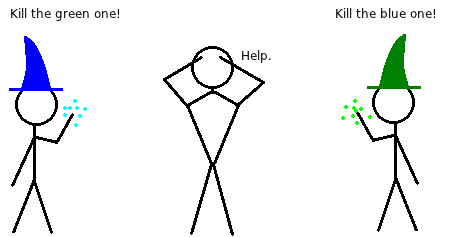
\includegraphics{Pics/Dominate.png}
\end{figure*}

You can control the actions of any humanoid creature through a telepathic link that you establish with the subject's mind.

If you and the subject have a common language, you can generally force the subject to perform as you desire, within the limits of its abilities. 
If no common language exists, you can communicate only basic commands, such as ``Come here,`` ``Go there,`` ``Fight,`` and ``Stand still.`` 
You know what the subject is experiencing, but you do not receive direct sensory input from it, nor can it communicate with you telepathically.

Once you have given a dominated creature a command, 
it continues to attempt to carry out that command to the exclusion of all other activities except those necessary for day-to-day survival 
(such as sleeping, eating, and so forth). 
Because of this limited range of activity, a Sense Motive check against DC 15 (rather than DC 25) 
can determine that the subject's behavior is being influenced by an enchantment effect (see the Sense Motive skill description).

Changing your instructions or giving a dominated creature a new command is the equivalent of redirecting a spell, so it is a move action.

By concentrating fully on the spell (a standard action), 
you can receive full sensory input as interpreted by the mind of the subject, though it still can't communicate with you. 
You can't actually see through the subject's eyes, so it's not as good as being there yourself, but you still get a good idea of what's going on.

Subjects resist this control, and any subject forced to take actions against its nature receives a new saving throw with a +2 bonus. 
Obviously self-destructive orders are not carried out. 
Once control is established, the range at which it can be exercised is unlimited, as long as you and the subject are on the same plane. 
You need not see the subject to control it.

If you don't spend at least 1 round concentrating on the spell each day, the subject receives a new saving throw to throw off the domination.

\nameref{Spell:AlignedProtection} or a similar spell can prevent you from exercising control or using the telepathic link while the subject is so warded, 
but such an effect neither prevents the establishment of domination nor dispels it.

\paragraph{Augment:} You can augment this spell in one or more of the following ways.
\begin{enumerate}
 \item If you spend 2 additional spell points, this spell can also affect an animal, fey, giant, magical beast, or monstrous humanoid.
 \item If you spend 4 additional spell points, this spell can also affect an aberration, 
 dragon, elemental, or outsider in addition to the creature types mentioned above.
 \item For every 2 additional spell points you spend, this spell can affect an additional target. 
 Any additional target cannot be more than 15 feet from another target of the spell.
 \item If you spend 1 additional spell point, this spell's duration changes to 1 hour.
 If you spend 2 additional spell points, this spell's duration changes to 1 day. 
 If you spend 4 additional spell points, this spell's duration changes to 1 day per caster level.
\end{enumerate}
\subsubsection{Dream}
\label{Spell:Dream}
Illusion (Phantasm) [Mind-Affecting]
\\ \textbf{Level:} Bard 5, Sor/Wiz 5
\\ \textbf{Components:} V, S
\\ \textbf{Casting Time:} 1 standard action
\\ \textbf{Range:} Unlimited
\\ \textbf{Target:} One creature
\\ \textbf{Duration:} Instantaneous; see text
\\ \textbf{Saving Throw:} Will negates; see text
\\ \textbf{Spell Resistance:} Yes
\\ \textbf{Spell Points:} 9

\emph{''Sleep tight. I'll be there.``}

You enter another creature's dream, either to deliver a message or to interrupt its sleep. These two functions of the spell work as follows:
\begin{itemize}
 \item \emph{Deliver message:} You send a ghostly avatar of yourself into the subject's dream, allowing you to communicate as if you were standing face to face.
 This communication happens instantaneously, regardless of how long the conversation is - time is irrelevant when dreaming.
 The conversation lasts for as long as you both desire - if one participant wishes the conversation to end, it ends.
 When the participants wake up, they remember the conversation perfectly.
 You cannot use any spells, magic items, or any class or racial features during this dream conversation. 
 However, the skills Bluff, Diplomacy, Disguise, Intimidate, Knowledge, Sense Motive and Speak Language work perfectly.
 \item \emph{Nightmare:} You send a hideous and unsettling phantasmal vision to a specific creature that you name or otherwise specifically designate.
 The nightmare prevents restful sleep, leaving the subject fatigued and unable to regain arcane spells for the next 24 hours. 
 A successful will save negates this effect.
 The difficulty of the save depends on how well you know the subject and what sort of physical connection (if any) you have to that creature.
 See the table (\ref{tab:Scrying}) accompanying the scrying spell.
 Using this function adds the [Evil] descriptor to the spell.
 A creature under the influence of an \nameref{Spell:AlignedProtection} spell is immune to this aspect of the spell.
\end{itemize}
If the recipient is awake when you cast the spell, you can choose to cease casting (ending the spell) or to enter a trance until the recipient goes to sleep, 
whereupon you become alert again and complete the casting. If you are disturbed during the trance, 
you must succeed on a Concentration check as if you were in the midst of casting a spell or the spell ends. 
If you choose to enter a trance, you are not aware of your surroundings or the activities around you while in the trance.
You are defenseless, both physically and mentally, while in the trance. (You always fail any saving throw, for example.)

Creatures who don't sleep (such as elves, but not half-elves) or dream cannot be affected by this spell. 

\textbf{Augment:} If you spend 8 additional spell points, the Nightmare function of the spell becomes truly deadly.
If the subject fails the Will saving throw, it must also make a Fortitude save using the same DC or die of fright, never waking up again.
This adds the [Death] descriptor to the spell, in addition to the [Mind-Affecting] and [Evil] descriptor it already has.
\subsubsection{Dweomer Blockade}
\label{Spell:DweomerBlockade}
Abjuration
\\ \textbf{Level:} Abjurer 6, Blackguard 6
\\ \textbf{Components:} V, S
\\ \textbf{Casting Time:} 1 standard action
\\ \textbf{Range:} Medium (100 ft. + 10 ft./level)
\\ \textbf{Effect:} Ray
\\ \textbf{Duration:} 1 min./level
\\ \textbf{Saving Throw:} Will negates
\\ \textbf{Spell Resistance:} No
\\ \textbf{Spell Points:} 11

\emph{A nearly translucent ray springs from your outstretched hand.} 

You must make a ranged touch attack to hit the target. 
Any creature or object struck by the ray that fails a Will save is treated as being entirely within an \nameref{Spell:AntimagicField}, including the effect such a field has on a creature's magic items.

\subsection{'E' Spells}
\subsubsection{Earthquake}
\label{Spell:Earthquake}
Evocation [Earth]
\\ \textbf{Level:} Destruction 7, Earth 7
\\ \textbf{Components:} V, S
\\ \textbf{Casting Time:} 1 standard action
\\ \textbf{Range:} Long (400 ft. + 40 ft./level)
\\ \textbf{Area:} 80-ft.-radius spread (S)
\\ \textbf{Duration:} 1 round
\\ \textbf{Saving Throw:} See text
\\ \textbf{Spell Resistance:} No
\\ \textbf{Spell Points:} 15

\emph{''Feel the ground tremble!``}

When you cast earthquake, an intense but highly localized tremor rips the ground. 
The shock knocks creatures down, collapses structures, opens cracks in the ground, and more. 
The effect lasts for 1 round, during which time creatures on the ground can't move or attack. 
A spellcaster on the ground must make a Concentration check (DC 20 + spell level) or lose any spell he or she tries to cast. 
The earthquake affects all terrain, vegetation, structures, and creatures in the area. 
The specific effect of an earthquake spell depends on the nature of the terrain where it is cast.

\begin{itemize}
\item \emph{Cave, Cavern, or Tunnel:}
The spell collapses the roof, dealing 8d6 points of bludgeoning damage to any creature caught under the cave-in (Reflex half) and pinning that creature beneath the rubble (see below).
An earthquake cast on the roof of a very large cavern could also endanger those outside the actual area but below the falling debris.

\item \emph{Cliffs:}
Earthquake causes a cliff to crumble, creating a landslide that travels horizontally as far as it fell vertically. 
Any creature in the path takes 8d6 points of bludgeoning damage (Reflex half) and is pinned beneath the rubble (see below).

\item \emph{Open Ground:}
Each creature standing in the area must make a Reflex save or fall prone. 
Additionally, fissures (each 10d10' deep) open in the earth. And every creature on the ground has a 25\% chance of falling into one (a second reflex save prevents the fall). 
At the end of the spell, all fissures grind shut, killing any creatures still trapped within.

\item \emph{Structure:}
Any structure standing on open ground takes 100 points of damage, enough to collapse a typical wooden or masonry building, but not a structure built of stone or reinforced masonry. 
Hardness does not reduce this damage, nor is it halved as damage dealt to objects normally is. 
Any creature caught inside a collapsing structure takes 8d6 points of bludgeoning damage (Reflex half) and is pinned beneath the rubble (see below).

\item \emph{River, Lake, or Marsh:}
Fissures open underneath the water, draining away the water from that area and forming muddy ground. 
Soggy marsh or swampland becomes quicksand for the duration of the spell, sucking down creatures and structures. 
Each creature in the area must make a Reflex save or sink down in the mud and quicksand. 
At the end of the spell, the rest of the body of water rushes in to replace the drained water, possibly drowning those caught in the mud.
\end{itemize}
Any creature pinned beneath rubble is \emph{immobilized} and takes 1d6 points of nonlethal damage per minute while pinned. 
If a pinned character falls unconscious, he or she must make a DC 15 Constitution check or take 1d6 points of lethal damage each minute thereafter until freed or dead.

\subsubsection{Endure Elements}
\label{Spell:EndureElements}
Abjuration
\\ \textbf{Level:} Blackguard 1, Paladin 1, Protection 1, Ranger 1, Sor/Wiz 1, Sun 1
\\ \textbf{Components:} V, S
\\ \textbf{Casting Time:} 1 standard action
\\ \textbf{Range:} Touch
\\ \textbf{Target:} Creature touched
\\ \textbf{Duration:} 24 hours
\\ \textbf{Saving Throw:} Will negates (harmless)
\\ \textbf{Spell Resistance:} Yes (harmless)
\\ \textbf{Spell Points:} 1

\emph{You fear no hail, drought, or storm.}

A creature protected by endure elements suffers no harm from being in a hot or cold environment. 
It can exist comfortably in conditions between -50 and 140 degrees Fahrenheit (between -45 and 60 degrees Celcius) without having to make Fortitude saves. 
The creature's equipment is likewise protected.

Endure elements doesn't provide any protection from fire or cold damage, 
nor does it protect against other environmental hazards such as smoke, lack of air, and so forth.

\paragraph{Augment:} You can augment this spell in one or more of the following ways.
\begin{enumerate}
\item If you spend two additional spell points, the subject of the spell does not treat slippery ice, areas of undergrowth, bogs or loose rubble as difficult terrain.
The subject does not have to pay extra movement in order to move through such terrain.
\item If you spend two additional spell points, the subject of the spell never risks catching on fire due to environmental fires.
\item If you spend two additional spell points, the subject of the spell is immune to the negative effects of environmental smoke and acid fume inhalation.
\end{enumerate}

\subsubsection{Energized Touch}
\label{Spell:ShockingGrasp}
Evocation [see text]%[Electricity]
\\ \textbf{Level:} Sor/Wiz 1
\\ \textbf{Components:} V, S
\\ \textbf{Casting Time:} 1 standard action
\\ \textbf{Range:} Touch
\\ \textbf{Target:} Creature or object touched
\\ \textbf{Duration:} Instantaneous
\\ \textbf{Saving Throw:} None
\\ \textbf{Spell Resistance:} Yes
\\ \textbf{Spell Points:} 1

\emph{*Zap!*}

\begin{figure*}
  \caption{Wizard incinerates unsuspecting victim at close range with \emph{Burning Hands}.}
  \centering
    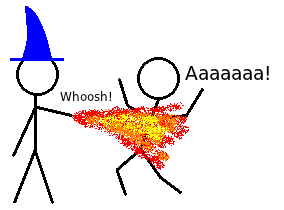
\includegraphics{Pics/BurningHands.png}
\end{figure*}

Your successful melee touch attack deals 1d8 points of energy damage. Choose one of the following energy types upon casting:
\begin{itemize}
 \item Cold: A touch of this energy type deals +1 point of damage per die. This form of the spell is usually referred to as \emph{Chill Touch}.
 \item Electricity: When delivering a jolt of this energy type, you gain a +3 bonus on attack rolls if the opponent is wearing metal armor 
 (or made out of metal, carrying a lot of metal, or the like), 
 and a +2 bonus on caster level checks for the purpose of overcoming spell resistance.
 This form of the spell is usually referred to as \emph{Shocking Grasp}.
 \item Fire: A touch of this energy type deals +1 point of damage per die.
 This form of the spell is usually referred to as \emph{Burning Hands}.
 \item Sonic: A touch of this energy type deals -1 point of damage per die and ignores an object's hardness.
\end{itemize}

This spell's descriptor is the same as the type of energy you selected. 

\paragraph{Augment:} For every additional spell point you spend, this spell's damage increases by one die (d8).

\emph{Special:} Casting this spell does not provoke Attacks of Opportunity.


\subsubsection{Energy Arrow}
\label{Spell:EnergyArrow}
Evocation [see text]
\\ \textbf{Level:} Sor/Wiz 3
\\ \textbf{Components:} V, S
\\ \textbf{Casting Time:} 1 standard action
\\ \textbf{Range:} Close (25 ft. + 5 ft./2 levels)
\\ \textbf{Target:} Fifty projectiles, all of which must be in contact with each other at the time of casting
\\ \textbf{Duration:} 10 min./level
\\ \textbf{Saving Throw:} None
\\ \textbf{Spell Resistance:} No
\\ \textbf{Spell Points:} 5

\emph{You hand the ranger back his quiver, its contents glowing with magical energy.}

You turn ammunition (such as arrows, bolts, shuriken, or stones) into magical projectiles. 
Each piece of ammunition gains the benefit of one of the following enhancements:
\emph{Flaming}, \emph{Frost} or \emph{Shock}.
You choose the energy type at the time of casting.
Multiple castings of this spell do not stack, even if different enhancements are selected - 
if you cast the spell a second time on a projectile
before the spell's duration expires, the previous casting is overridden with respect to that projectile.
This allows the ammunition to bypass damage reduction as
if they were magic weapons, but they do not actually gain an enhancement bonus
(unless, of course, they are fired from a magical missile weapon).

This spell's descriptor matches the type of energy you imbue the projectiles with.

\paragraph{Augment:} If you spend 4 additional spell points, 
you can instead select from one of the following enhancements:
\emph{Flaming Burst}, \emph{Icy Burst}, and \emph{Shocking Burst}.

\subsubsection{Energy Ball}
\label{Spell:EnergyBall}
Evocation [see text]
\\ \textbf{Level:} Magic 2, Sor/Wiz 2
\\ \textbf{Components:} V, S
\\ \textbf{Casting Time:} 1 standard action
\\ \textbf{Range:} Long (400 ft. + 40 ft./level)
\\ \textbf{Area:} 20-ft.-radius burst
\\ \textbf{Duration:} Instantaneous
\\ \textbf{Saving Throw:} Reflex half or Fortitude half; see text
\\ \textbf{Spell Resistance:} Yes
\\ \textbf{Spell Points:} 3

\emph{If the explosion didn't solve your problem, try a bigger one.}

An Energy Ball spell is an explosion of energy that detonates with a low roar and deals 3d6 points of damage to every creature within the area. 
Unattended objects also take this damage. 

You choose between cold, electricity, fire, or sonic damage at the time of casting.
If the damage caused to an interposing barrier shatters or breaks through it, the Ball may continue beyond the barrier if the area permits; 
otherwise it stops at the barrier just as any other spell effect does. 

You point your finger and determine the range (distance and height) at which the Ball is to burst. 
A glowing, pea-sized bead streaks from the pointing digit and, unless it impacts upon a material body or solid barrier prior to attaining the prescribed range, 
blossoms into the Ball at that point. (An early impact results in an early detonation.)

\begin{itemize}
 \item Cold: A burst of this energy type deals +1 point of damage per die. 
 The saving throw to reduce damage from a cold burst is a Fortitude save instead of a Reflex save.
 \item Electricity: A burst of this energy type provides a +2 bonus to the save DC
 and a +2 bonus on caster level checks for the purpose of overcoming spell resistance.
 \item Fire: A burst of this energy type deals +1 point of damage per die.
 \item Sonic: A burst of this energy type deals -1 point of damage per die and ignores an object's hardness.
\end{itemize}
The spell has all side effects you would normally expect a flash of energy to produce - fire causes small, flammable objects to catch fire, cold causes exposed bodies of water to get a thin coating of ice, and so on.
The explosion also creates significant pressure, which has effects of its own. 
Light, unattended objects are hurled away from the blast radius, and glass windows may break.

This spell's descriptor is the same as the type of energy you selected. 

\paragraph{Augment:} For every additional spell point you spend, this spell's damage increases by one die (d6).

\subsubsection{Energy Bolt}
\label{Spell:EnergyBolt}
Evocation [see text]
\\ \textbf{Level:} Destruction 2, Sor/Wiz 2
\\ \textbf{Components:} V, S
\\ \textbf{Casting Time:} 1 standard action
\\ \textbf{Range:} 120 ft.
\\ \textbf{Area:} 120-ft. line
\\ \textbf{Duration:} Instantaneous
\\ \textbf{Saving Throw:} Reflex half or Fortitude half; see text
\\ \textbf{Spell Resistance:} Yes
\\ \textbf{Spell Points:} 3

\emph{''Fancy spells are good and all, but there's something to be said about just lancing out with energy.``}

You release a powerful stroke of energy that deals 3d6 points of damage to every creature within the area. The bolt begins at your fingertips.
Unattended objects also take this damage.

You choose between cold, electricity, fire, or sonic damage at the time of casting.
If the damage caused to an interposing barrier shatters or breaks through it, the bolt may continue beyond the barrier if the spell's range permits; otherwise, it stops at the barrier just as any other spell effect does.

\begin{itemize}
 \item Cold: A bolt of this energy type deals +1 point of damage per die. 
 The saving throw to reduce damage from a cold bolt is a Fortitude save instead of a Reflex save.
 \item Electricity: A bolt of this energy type provides a +2 bonus to the save DC
 and a +2 bonus on caster level checks for the purpose of overcoming spell resistance.
 \item Fire: A bolt of this energy type deals +1 point of damage per die.
 \item Sonic: A bolt of this energy type deals -1 point of damage per die and ignores an object's hardness.
\end{itemize}
The spell has all side effects you would normally expect a flash of energy to produce - electricity or fire can melt metals with a low melting point, such as lead, gold, copper, silver, or bronze, and so on.

This spell's descriptor is the same as the type of energy you selected.

\paragraph{Augment:} You can augment this spell in one or both of the following ways:
\begin{enumerate}
 \item For every additional spell point you spend, this spell's damage increases by one die (d6).
 \item For every additional spell point you spend, this spell's range and length of the area increases by 10'.
\end{enumerate}

\subsubsection{Enervation}
\label{Spell:Enervation}
Necromancy
\\ \textbf{Level:} Necromancer 4
\\ \textbf{Components:} V, S
\\ \textbf{Casting Time:} 1 standard action
\\ \textbf{Range:} Close (25 ft. + 5 ft./2 levels)
\\ \textbf{Effect:} Ray of negative energy
\\ \textbf{Duration:} Instantaneous
\\ \textbf{Saving Throw:} None
\\ \textbf{Spell Resistance:} Yes
\\ \textbf{Spell Points:} 7

\emph{You point your finger and utter the incantation, releasing a black ray of crackling negative energy that suppresses the life force of any living creature it strikes.} 

You must make a ranged touch attack to hit.
If the attack succeeds, the subject gains 1d4 negative levels.

If the subject has at least as many negative levels as HD, it dies. 

Each negative level gives a creature a -1 penalty on attack rolls, saving throws, 
skill checks, ability checks, and effective level (for determining the power, duration, DC, and other details of spells or special abilities), 
and causes it to lose 5 hit points.
Spellcasters take additional penalties, as detailed under the \nameref{sec:NegativeLevels} section.

Assuming the subject survives, it regains lost levels after 1 hour. 
Usually, negative levels have a chance of permanently draining the victim's levels,
but the negative levels from enervation don't last long enough to do so.

An undead creature struck by the ray gains 1d4$\times$5 temporary hit points for 1 hour.

\paragraph{Augment:} For every 3 additional spell points you spend, this spell inflicts an additional negative level on a successful hit.
\subsubsection{Entangle}
\label{Spell:Entangle}
Transmutation
\\ \textbf{Level:} Plant 1, Ranger 1
\\ \textbf{Components:} V, S
\\ \textbf{Casting Time:} 1 standard action
\\ \textbf{Range:} Long (400 ft. + 40 ft./level)
\\ \textbf{Area:} Plants in a 20-ft.-radius spread
\\ \textbf{Duration:} 1 min./level (D)
\\ \textbf{Saving Throw:} Reflex partial; see text
\\ \textbf{Spell Resistance:} No
\\ \textbf{Spell Points:} 1

\emph{Grasses, weeds, bushes, and even trees wrap, twist, and entwine about everything in their path.} 

Creatures in the area or those that enter it are \emph{entangled}.
The creature can break free and move half its normal speed by using a full-round action to make a DC 20 Strength check or a DC 20 Escape Artist check. 
A creature that succeeds on a Reflex save is not entangled but can still move at only half speed through the area. 
Each round on your turn, the plants once again attempt to entangle all creatures that have avoided or escaped entanglement.

\paragraph{Augment:} If you spend 8 additional spell points, creatures in the area are \emph{immobilized} on a failed save rather than \emph{entangled}. The Strength or Escape Artist check DCs are not affected.

\subsubsection{Enthrall}
\label{Spell:Enthrall}
Enchantment (Charm) [Language Dependent, Mind-Affecting, Sonic]
\\ \textbf{Level:} Bard 2, Cleric 2
\\ \textbf{Components:} V, S
\\ \textbf{Casting Time:} 1 round
\\ \textbf{Range:} Medium (100 ft. + 10 ft./level)
\\ \textbf{Targets:} Any number of creatures
\\ \textbf{Duration:} 1 hour or less; see text
\\ \textbf{Saving Throw:} Will negates; see text
\\ \textbf{Spell Resistance:} Yes
\\ \textbf{Spell Points:} 3

\emph{''I have a dream. Ich bin ein Berliner! Now this is not the end, it is not even the beginning of the end!}

If you have the attention of a group of creatures, you can use this spell to hold them spellbound. To cast the spell, you must speak or sing without interruption for 1 full round. 

Those affected give you their undivided attention thereafter, ignoring their surroundings. They are considered to have an attitude of friendly while under the effect of the spell.

A creature with more HD than your caster level remains aware of its surroundings and has an attitude of indifferent. It gains a new saving throw if it witnesses actions that it opposes.

The effect lasts as long as you speak or sing, to a maximum of 1 hour. Those enthralled by your words take no action while you speak or sing and for 1d3 rounds thereafter while they discuss the topic or performance. Those entering the area during the performance must also successfully save or become enthralled. 

The speech ends (but the 1d3-round delay still applies) if you lose concentration or do anything other than speak or sing.

If those not enthralled have unfriendly or hostile attitudes toward you, they can collectively make a Charisma check to try to end the spell by jeering and heckling. For this check, use the Charisma bonus of the creature with the highest Charisma in the group; others may make Charisma checks to assist. The heckling ends the spell if this check result beats your Charisma check result. Only one such challenge is allowed per use of the spell.

If any member of the audience is attacked or subjected to some other overtly hostile act, the spell ends and the previously enthralled members become immediately unfriendly toward you.

\emph{Note:} Clerics usually refer to this spell as \emph{Mass} rather than \emph{Enthrall}.
\subsubsection{Entropic Shield}
\label{Spell:EntropicShield}
Abjuration
\\ \textbf{Level:} Air 1, Luck 1
\\ \textbf{Components:} V, S
\\ \textbf{Casting Time:} 1 standard action
\\ \textbf{Range:} Personal
\\ \textbf{Target:} You
\\ \textbf{Duration:} 1 min./level (D)
\\ \textbf{Spell Points:} 1

\emph{A magical field appears around you, glowing with a chaotic blast of multicolored hues, deflecting incoming arrows, rays, and other ranged attacks.} 
 
Each ranged attack directed at you for which the attacker must make an attack roll (including a touch attack) has a 20\% miss chance.
This miss chance is not concealment. When a creature is under both concealment and Entropic Shield, use only the larger percentage miss chance.
Other attacks that simply work at a distance are not affected.

\paragraph{Augment:} For every additional spell point you spend, the miss chance offered by this spell increases by 5\%, to a maximum of 50\% for a 9-point additional expenditure.
\subsubsection{Ethereal Jaunt}
\label{Spell:EtherealJaunt}
Transmutation
\\ \textbf{Level:} Sor/Wiz 7
\\ \textbf{Components:} V, S
\\ \textbf{Casting Time:} 1 standard action
\\ \textbf{Range:} Touch
\\ \textbf{Target:} Creature touched
\\ \textbf{Duration:} 1 round/level (D)
\\ \textbf{Saving Throw:} Will negates
\\ \textbf{Spell Resistance:} Yes
\\ \textbf{Spell Points:} 13

\emph{The creature fades out of sight with the sound of someone exhaling softly.}

The subject becomes ethereal, along with your equipment. 
For the duration of the spell, the subject is in a place called the Ethereal Plane, which overlaps the normal, physical, Material Plane. 
When the spell expires, the subjects return to material existence.

An ethereal creature is invisible, insubstantial, and capable of moving in any direction, even up or down, albeit at half normal speed. 
An insubstantial creature can move through solid objects, including living creatures. 
An ethereal creature can see and hear on the Material Plane, but everything looks gray and ephemeral. 
Sight and hearing onto the Material Plane are limited to 60 feet.
Force effects and abjurations affect an ethereal creature normally. 
Their effects extend onto the Ethereal Plane from the Material Plane, but not vice versa. 
An ethereal creature can't attack material creatures, and spells you cast while ethereal affect only other ethereal things. 
Certain material creatures or objects have attacks or effects that work on the Ethereal Plane.
Treat other ethereal creatures and ethereal objects as if they were material.

If you end the spell while the subject is inside a material object (such as a solid wall), 
the subject is shunted off to the nearest open space and takes 1d6 points of damage per 5 feet that you so travel. 

\paragraph{Augment:} You can augment this spell in one or both of the following ways:
\begin{enumerate}
 \item For every two additional spell points you spend, this spell can affect an additional creature.
 \item If you spend two additional spell points, this spell's duration increases to 1 min./level.
\end{enumerate}
\subsubsection{Eyebite}
\label{Spell:Eyebite}
Necromancy [\nameref{sec:Curses}], Evil]
\\ \textbf{Level:} Bard 6, Sor/Wiz 6
\\ \textbf{Components:} V, S
\\ \textbf{Casting Time:} 1 standard action
\\ \textbf{Range:} Close (25 ft. + 5 ft./2 levels)
\\ \textbf{Target:} One living creature
\\ \textbf{Duration:} Instantaneous; see text
\\ \textbf{Saving Throw:} Will negates
\\ \textbf{Spell Resistance:} Yes
\\ \textbf{Spell Points:} 11

\emph{''The evil eye is not a myth, as you will now learn to understand!``}

Each round, you may target a single living creature, striking it with waves of evil power.
Depending on the target's HD, this attack has as many as three effects. See the \nameref{tab:Eyebite} table for information on which effects apply.
The effects are concurrent.

\begin{tableonecolumn}
\caption{Eyebite}
\label{tab:Eyebite}
\begin{tabular}{ll}
\toprule
HD&Effect\\
\midrule
10 or more&Sickened\\
9 or less&Panicked, sickened\\
4 or less&Comatose, panicked, sickened\\
\bottomrule
\end{tabular}\\
\end{tableonecolumn}
The effects are:

\textbf{Sickened:} Sudden pain and fever sweeps over the subject's body, rendering it \emph{sickened}.
A creature affected by this spell remains sickened for 10 minutes per caster level. 
The effects cannot be negated by a Remove Disease or \nameref{Spell:Heal} spell.

\textbf{Panicked:} The subject becomes \emph{panicked} for 1d4 rounds. 
Even after the panic ends, the creature remains shaken for 10 minutes per caster level, and 
it automatically becomes panicked again if it comes within sight of you during that time. 
This is a fear effect (it is possible to be immune to this part of the spell, while still being subject to the others normally).

\textbf{Comatose:} The subject falls into a catatonic coma for 10 minutes per caster level. 
During this time, it cannot be awakened by any means short of removing the curse.
This is not a sleep effect, and thus elves are not immune to it.

The spell lasts for 1 round per three caster levels. You must spend a move action each round after the first to target a foe. 

This spell can not be dispelled, but see \nameref{sec:RemovingACurse}.

\paragraph{Augment:} You affect creatures more powerfully by spending additional spell points.
For each additional spell point you spend, a creature of 1 HD more is affected by the Panicked and Comatose effects of the spell.
For example, if you spend one additional spell point, a creature of 10 HD or less is Panicked and Sickened, and a creature of 5 HD or less is Comatose, Panicked, and Sickened.
\subsubsection{Expeditious Retreat}
\label{Spell:ExpeditiousRetreat}
Transmutation
\\ \textbf{Level:} Bard 1, Ranger 1, Sor/Wiz 1, Travel 1
\\ \textbf{Components:} V, S
\\ \textbf{Casting Time:} 1 standard action or 1 swift action; see text
\\ \textbf{Range:} Personal
\\ \textbf{Target:} You
\\ \textbf{Duration:} 1 min./level (D) or 1 round; see text
\\ \textbf{Spell Points:} 1

\emph{Each of your steps takes you a much farther distance than they by any rights should.}

All of the subject's modes of movement (including land movement, burrow, climb, fly, and swim) increase by 30 feet. This increase counts as an enhancement bonus, and it affects the subject's jumping distance as normal for increased speed. The spell does not grant new kinds of movement, it merely enhances those the subject already has.

At the time of casting, you make a choice. If you cast the spell as a standard action, the duration is 1 minute per level. 
If you cast it as a swift action, the duration is one round.

\paragraph{Augment:}  You can augment this spell in one or both of the following ways.
\begin{enumerate}
 \item For every 2 additional spell points you spend, the bonus to your speeds increases by 10'.
 \item If you spend 2 additional spell points, the spell's range changes to ''touch``, and the target changes to ''creature touched``. 
\end{enumerate}
\subsubsection{Explosive Runes}
\label{Spell:ExplosiveRunes}
Abjuration [Force]
\\ \textbf{Level:} Sor/Wiz 3
\\ \textbf{Components:} V, S
\\ \textbf{Casting Time:} 1 standard action
\\ \textbf{Range:} Touch
\\ \textbf{Target:} One touched object weighing no more than 10 lb.
\\ \textbf{Duration:} Permanent until discharged (D)
\\ \textbf{Saving Throw:} See text
\\ \textbf{Spell Resistance:} Yes

\emph{''Have a nice day, I have rigged this piece of paper to explode.``}

You trace these mystic runes upon a book, map, scroll, or similar object bearing written information. 
The runes detonate when read, dealing 5d6 points of force damage. 
Anyone next to the runes (close enough to read them) takes the full damage with no saving throw; 
any other creature within 10 feet of the runes is entitled to a Reflex save for half damage. 
The object on which the runes were written also takes full damage (no saving throw).
Any other objects within the 10 foot radius that carry another instance of the explosive runes
are burned out, the explosive runes disappating harmlessly.

You and any characters you specifically instruct can read the protected writing without triggering the runes. 
Likewise, you can remove the runes whenever desired. 
Another creature can remove them with a successful \nameref{Spell:DispelMagic} spell %or erase spell, 
but attempting to dispel the runes and failing to do so triggers the explosion.
Since you automatically succeed on all dispel checks against spells you cast yourself, 
you cannot trigger your own explosive runes with \nameref{Spell:DispelMagic}.

Note: Magic traps such as explosive runes are hard to detect and disable. 
A rogue (only) can use the Search skill to find the runes and Disable Device to thwart them. 
The DC in each case is 25 + spell level, or 28 for explosive runes.

\paragraph{Augment:} For every additional spell point you spend, this spell's damage increases by 1d6.
%In addition, for every two spell points you spend to improve the spell's damage, its saving throw DC increases by 1.
\subsection{'F' Spells}
\subsubsection{Faerie Fire}
\label{Spell:FaerieFire}
Evocation [Light]
\\ \textbf{Level:} Fire 1
\\ \textbf{Components:} V, S
\\ \textbf{Casting Time:} 1 standard action
\\ \textbf{Range:} Long (400 ft. + 40 ft./level)
\\ \textbf{Area:} Creatures and objects within a 5-ft.-radius burst
\\ \textbf{Duration:} 1 min./level (D)
\\ \textbf{Saving Throw:} None
\\ \textbf{Spell Resistance:} Yes
\\ \textbf{Spell Points:} 1

\emph{A pale glow surrounds the subjects.} 

All creatures within the burst are outlined, and shed light as candles. 
Outlined creatures do not benefit from the concealment normally provided by darkness (though a magical darkness effect functions normally if more spell points were spent on the darkness effect than on the Faerie Fire spell), \nameref{Spell:Blur}, \emph{invisibility}, or similar effects. 
The light is too dim to have any special effect on undead or dark-dwelling creatures vulnerable to light. 
The faerie fire can be blue, green, or violet, according to your choice at the time of casting. 
The faerie fire does not cause any harm to the objects or creatures thus outlined.

\paragraph{Augment:} This spell can be augmented in one or both of the following ways:
\begin{enumerate}
 \item For every additional spell point you spend, you can create an additional 5' radius burst of Faerie Fire to erupt somewhere within range. The bursts need not be adjacent to one another.
 \item If you spend 4 additional spell points, creatures subjected to the burst must make a successful Will saving throw or lose their Dexterity bonus to AC for 1d4+1 rounds due to disorientation. This is in addition to the dust's normal effects.
\end{enumerate}
\subsubsection{False Life}
\label{Spell:FalseLife}
Necromancy
\\ \textbf{Level:} Assassin 3, Blackguard 2, Sor/Wiz 2
\\ \textbf{Components:} V, S
\\ \textbf{Casting Time:} 1 standard action
\\ \textbf{Range:} Personal
\\ \textbf{Target:} You
\\ \textbf{Duration:} 1 hour/level or until depleted; see text
\\ \textbf{Spell Points:} Assassin 5, Blackguard 3, Sor/Wiz 3

\emph{You harness the power of unlife to grant yourself a limited ability to avoid death.} 

While this spell is in effect, you gain 1d10 temporary hit points, plus one point per caster level.

\paragraph{Augment:} Every 2 additional spell points spent increase the temporary hit points you gain by 1d10.

\subsubsection{False Vision}
\label{Spell:FalseVision}
Illusion (Glamer)
\\ \textbf{Level:} Bard 5, Sor/Wiz 5, Trickery 5
\\ \textbf{Components:} V, S
\\ \textbf{Casting Time:} 1 standard action
\\ \textbf{Range:} Touch
\\ \textbf{Area:} 40-ft.-radius emanation
\\ \textbf{Duration:} 1 hour/level (D)
\\ \textbf{Saving Throw:} None
\\ \textbf{Spell Resistance:} No
\\ \textbf{Spell Points:} 9

\emph{''If they are looking, they will be in for a surprise.``}

Any divination (scrying) spell used to view anything within the area of this spell instead receives a false image, as defined by you at the time of casting. 
The false image the scryer sees functions as if generated by an \nameref{Spell:Image} spell, augmented with as many points as were spent on casting the
False Vision spell.
As long as the duration lasts, you can concentrate to change the image as desired. 
While you aren't concentrating, the image remains static.
\subsubsection{Feeblemind}
\label{Spell:Feeblemind}
Enchantment (Compulsion) [Mind-Affecting]
\\ \textbf{Level:} Sor/Wiz 5
\\ \textbf{Components:} V, S
\\ \textbf{Casting Time:} 1 standard action
\\ \textbf{Range:} Medium (100 ft. + 10 ft./level)
\\ \textbf{Target:} One creature
\\ \textbf{Duration:} Instantaneous
\\ \textbf{Saving Throw:} Will negates; see text
\\ \textbf{Spell Resistance:} Yes
\\ \textbf{Spell Points:} 9

\emph{''Not so smart now, Mr. Wizard?``}

If the target creature fails a Will saving throw, its Intelligence and Charisma scores each drop to 1. 
The affected creature is unable to use Intelligence- or Charisma-based skills, cast spells, understand language, or communicate coherently. 
Still, it knows who its friends are and can follow them and even protect them. 
The subject remains in this state until a \nameref{Spell:Heal}, \nameref{Spell:LimitedWish} , 
\nameref{Spell:Miracle}, or \nameref{Spell:Wish} spell is used to cancel the effect of the feeblemind. 
A creature that can cast arcane spells, such as a sorcerer or a wizard, takes a -4 penalty on its saving throw.

\subsubsection{Fear}
\label{Spell:Fear}
Necromancy [Fear, Mind-Affecting]
\\ \textbf{Level:} Bard 1, Blackguard 1, Death 1, Evil 1, Necromancer 1
\\ \textbf{Components:} V, S
\\ \textbf{Casting Time:} 1 standard action
\\ \textbf{Range:} Close (25 ft. + 5 ft./2 levels)
\\ \textbf{Target:} One living creature with 5 or fewer HD
\\ \textbf{Duration:} 1d4 rounds or 1 round; see text
\\ \textbf{Saving Throw:} Will partial
\\ \textbf{Spell Resistance:} Yes
\\ \textbf{Spell Points:} 1

\emph{You raise your hand and intone words of dread.}

The affected creature becomes \emph{frightened}. 
If the subject succeeds on a Will save, it is instead \emph{shaken} for 1 round. 
Creatures with 6 or more Hit Dice cannot be \emph{frightened} by this spell, only becoming \emph{shaken} even on a failed save.

\paragraph{Augment:} You can augment this spell in one or more of the following ways.
\begin{enumerate}
\item If you spend two additional spell points, the range of the spell increases to Medium.
\item For every two additional spell points spent, the spell can affect an additional creature.
\item If you spend two additional spell points, instead of becoming \emph{frightened} on a failed save, the subject becomes \emph{panicked}.
\end{enumerate}
In addition, for every additional spell point spent on augmenting the spell, the spell can \emph{frighten} a creature with one more HD.
\subsubsection{Fiendish Flight}
\label{Spell:FiendishFlight}
Transmutation [Evil]
\\ \textbf{Level:} Blackguard 3

\emph{The subject grows large batlike wings.}

This spell functions as the \nameref{Spell:Fly} spell (including its augmentation option), except as noted here, and that the flight is due to physical wings the subject grows (which matters for effects like those caused by tanglefoot bags).

\subsubsection{Fireball}
\label{Spell:Fireball}
Evocation [Fire]
\\ \textbf{Level:} Evoker 2
\\ \textbf{Components:} V, S
\\ \textbf{Casting Time:} 1 standard action
\\ \textbf{Range:} Long (400 ft. + 40 ft./level)
\\ \textbf{Area:} 20-ft.-radius spread
\\ \textbf{Duration:} Instantaneous
\\ \textbf{Saving Throw:} Reflex half
\\ \textbf{Spell Resistance:} Yes
\\ \textbf{Spell Points:} 3

\emph{If the explosion didn't solve your problem, try a bigger one.}

A Fireball is a more specialized form of the \nameref{Spell:EnergyBall} spell, favored by Evokers. It deals 3d6+3 points of fire damage to every creature within the area. Unattended objects also take this damage. 

Unlike Energy Ball, Fireball is a spread, turning corners and negating many forms of cover.

Like Energy Ball, you point your finger and determine the range (distance and height) at which the Fireball is to explode. 
A glowing, pea-sized bead streaks from the pointing digit and, unless it impacts upon a material body or solid barrier prior to attaining the prescribed range, blossoms into the Fireball at that point. (An early impact results in an early detonation.)

The spell has all side effects you would normally expect a flash of fire to produce. The explosion also creates significant pressure, which has effects of its own. Light, unattended objects are hurled away from the blast radius, and glass windows may break.

\paragraph{Augment:} For every additional spell point you spend, this spell's damage increases by 1d6+1.

\emph{Special:} Fireballs, nearly filling the affected area, are extraordinarily hard to dodge. The base saving throw DC against a Fireball spell is 10 + the number of spell points spent on the spell and its augments + your key ability modifier, rather than as described in the section on \nameref{sec:SavingThrow}s.
\subsubsection{Fire Seeds}
\label{Spell:FireSeeds}
Conjuration (Creation) [Fire]
\\ \textbf{Level:} Fire 6, Sun 6
\\ \textbf{Components:} V, S
\\ \textbf{Casting Time:} 1 standard action
\\ \textbf{Range:} Touch
\\ \textbf{Targets:} Up to four touched acorns or up to eight touched holly berries
\\ \textbf{Duration:} 10 min./level or until used
\\ \textbf{Saving Throw:} None or Reflex half; see text
\\ \textbf{Spell Resistance:} No
\\ \textbf{Spell Points:} 11

\emph{You channel fire into the seeds until they are about to burst.}

Depending on the version of fire seeds you choose, you turn acorns into splash weapons that you or another character can throw, or you turn holly berries into bombs that you can detonate on command. Each version has separate augmentation options.

\begin{itemize}
 \item \emph{Acorn Grenades:} As many as four acorns turn into special splash weapons that can be hurled as far as 100 feet. A ranged touch attack roll is required to strike the intended target. Together, the acorns are capable of dealing 11d6 points of fire damage, divided up among the acorns as you wish (in increments of one die of damage).

Each acorn explodes upon striking any hard surface. In addition to its regular fire damage, it deals 1 point of splash damage per die, and it ignites any combustible materials within 10 feet. A creature within this area that makes a successful Reflex saving throw takes only half damage; a creature struck directly is not allowed a saving throw.
\paragraph{Augment:} For every additional spell point you spend on the \emph{Acorn Grenades} version of the spell, the combined damage dealt by the grenades increases by one die (d6).
 \item \emph{Holly Berry Bombs:} You turn as many as eight holly berries into special bombs. 
The holly berries are usually placed by hand, since they are too light to make effective thrown weapons (they can be tossed only 5 feet). If dropped from a height, use the rules for aiming splash weapons at a square. If you are within 200 feet and speak a word of command (a standard action), each berry instantly bursts into flame, causing 1d8+11 points of fire damage to every creature in a 5-foot radius burst and igniting any combustible materials within 5 feet. A creature in the area that makes a successful Reflex saving throw takes only half damage.
\paragraph{Augment:} For every additional spell point you spend on the \emph{Holly Berry Bombs} version of the spell, each bomb deals an additional point of fire damage.
\end{itemize}
\subsubsection{Fire Storm}
\label{Spell:FireStorm}
Evocation [Fire]
\\ \textbf{Level:} Fire 7
\\ \textbf{Components:} V, S
\\ \textbf{Casting Time:} 1 standard action
\\ \textbf{Range:} Medium (100 ft. + 10 ft./level)
\\ \textbf{Area:} Two 10-ft. cubes per level (S) OR cone-shaped burst out to 10' per level OR sphere-shaped burst centered on you out to 5' per level
\\ \textbf{Duration:} Instantaneous
\\ \textbf{Saving Throw:} Reflex half
\\ \textbf{Spell Resistance:} Yes
\\ \textbf{Spell Points:} 13

\emph{The whole area is shot through with sheets of roaring flame.} 

A Fire Storm can take one of three shapes, chosen at the time of casting.

Creatures within the chosen area take 13d6+13 points of fire damage. A successful Reflex saving throw halves this damage.

The spell does not harm natural vegetation or ground cover unless you so desire.

\paragraph{Augment:} You can augment this spell in one or both of the following ways:
\begin{enumerate}
 \item For every additional spell point you spend, this spell's damage increases by d6+1.
 \item If you spend 2 additional spell points, you can select any number of creatures within the spell area to specifically exclude them from damage.
\end{enumerate}
\subsubsection{Finger of Death}
\label{Spell:FingerOfDeath}
Necromancy [Death]
\\ \textbf{Level:} Death 7, Sor/Wiz 7
\\ \textbf{Components:} V, S
\\ \textbf{Casting Time:} 1 standard action
\\ \textbf{Range:} Close (25 ft. + 5 ft./2 levels)
\\ \textbf{Target:} One living creature
\\ \textbf{Duration:} Instantaneous
\\ \textbf{Saving Throw:} Fortitude partial
\\ \textbf{Spell Resistance:} Yes
\\ \textbf{Spell Points:} 13

\emph{``AVADA KEDAVRA!''}

You can slay any one living creature within range. 
The target is entitled to a Fortitude saving throw to survive the attack. 
If the save is successful, the creature instead takes 3d6 points of damage +1 point per caster level.

The subject might die from damage even if it succeeds on its saving throw. 

\paragraph{Augment:} For every 3 additional spell points you spend, this spell can target an additional creature within range.
\subsubsection{Fist of the Deity}
\label{Spell:FistOfTheDeity}
Evocation [see text]
\\ \textbf{Level:} Chaos 4, Evil 4, Good 4, Law 4
\\ \textbf{Components:} V, S
\\ \textbf{Casting Time:} 1 standard action
\\ \textbf{Range:} Medium (100 ft. + 10 ft./level)
\\ \textbf{Area:} 20-ft.-radius burst
\\ \textbf{Duration:} Instantaneous; see text
\\ \textbf{Saving Throw:} Will partial; see text
\\ \textbf{Spell Resistance:} Yes
\\ \textbf{Spell Points:} 7

\emph{You blast the area with energy, but only the unworthy must fear.}

When casting this spell, select an alignment. The spell gains a descriptor matching that alignment.

Any creature within the spell's area not of the selected aligment takes 4d8 points of damage, 
unless it is an outsider with an alignment subtype of the alignment opposed to the alignment you selected,
in which case it takes 7d6 points of damage.
In addition, all creatures not of the selected alignment suffer an additional penalty, depending on the alignment you selected:
\begin{itemize}
 \item \emph{Chaos:} The chaotic version of this spell is referred to as \emph{Chaos Hammer}, and stuns creatures for 1d2 rounds.
 \item \emph{Evil:} The evil version of this spell is referred to as \emph{Unholy Blight}, and blinds creatures for 2d4 rounds.
 \item \emph{Good:} The good version of this spell is referred to as \emph{Holy Smite}, and nauseates creatures for 1d4 rounds.
 \item \emph{Law:} The lawful version of this spell is referred to as \emph{Order's Wrath}, and dazes creatures for 1d2 rounds.
\end{itemize}
A successful will saving throw reduces the damage by half and negates the additional penalty.

\paragraph{Augment:} For every 2 additional spell points you spend, 
the damage against outsiders of an opposed alignment increases by 2d6, 
and the damage against other creatures increases by 1d8.
\subsubsection{Flame Blade}
\label{Spell:FlameBlade}
Conjuration (Creation) [Fire]
\\ \textbf{Level:} Fire 2
\\ \textbf{Components:} V, S
\\ \textbf{Casting Time:} 1 standard action
\\ \textbf{Range:} 0 ft.
\\ \textbf{Effect:} A weapon made of fire
\\ \textbf{Duration:} 1 min./level (D)
\\ \textbf{Saving Throw:} None
\\ \textbf{Spell Resistance:} No
\\ \textbf{Spell Points:} 3

\emph{You cause a blazing beam of red-hot fire to spring from your hand and solidify.}

You conjure a weapon made of pure, solidified fire.
This can be any kind of melee weapon with which you are proficient.

The weapon functions as a normal, physical weapon of its kind, except that all damage it deals is converted to fire damage\footnote{If you have access to the Fire domain, some of the damage may be again converted to divine damage.}.

No one but you can use this weapon. If someone successfully disarms you of the weapon, it immediately disappears in a burst of flame that deals 1d6 points of fire damage to the one that disarmed you of it.
The weapon then reforms in your hands at the start of your next turn.
The weapon cannot be sundered or otherwise damaged (though it can be dispelled).

The weapon can be improved by spells and other effects that affect normal weapons, such as the \nameref{Spell:MagicWeapon} spell (but not by actual magical enhancements, since the weapon doesn't last long enough to have those placed on it). 

\paragraph{Augment:} This spell can be augmented in one or both of the following ways:
\begin{enumerate}
 \item For every 3 additional spell points you spend, the weapon deals 1d6 points of fire damage in addition to its normal (converted) damage.
 \item If you spend 6 additional spell points, this spell's casting time changes to 1 swift action.
\end{enumerate}
\subsubsection{Flame Strike}
\label{Spell:FlameStrike}
Evocation [Fire]
\\ \textbf{Level:} Fire 4, Sun 4, War 4
\\ \textbf{Components:} V, S
\\ \textbf{Casting Time:} 1 standard action
\\ \textbf{Range:} Medium (100 ft. + 10 ft./level)
\\ \textbf{Area:} Cylinder (10-ft. radius, 40 ft. high)
\\ \textbf{Duration:} Instantaneous
\\ \textbf{Saving Throw:} Reflex partial; see text
\\ \textbf{Spell Resistance:} Yes
\\ \textbf{Spell Points:} 9

\emph{A vertical column of divine fire roars downward.}

The spell deals 7d6 points of fire damage, and knocks every creature within the area prone.
A successful reflex save reduces the damage by half, and prevents the creature from being knocked down.

\paragraph{Augment:} For every additional spell point you spend on this spell, its damage is increased by one die (d6).
\subsubsection{Flaming Sphere}
\label{Spell:FlamingSphere}
Evocation [Fire]
\\ \textbf{Level:} Fire 2, Sor/Wiz 2
\\ \textbf{Components:} V, S
\\ \textbf{Casting Time:} 1 standard action
\\ \textbf{Range:} Medium (100 ft. + 10 ft./level)
\\ \textbf{Effect:} 5-ft.-diameter sphere
\\ \textbf{Duration:} 1 round/level
\\ \textbf{Saving Throw:} None
\\ \textbf{Spell Resistance:} Yes
\\ \textbf{Spell Points:} 3

\emph{A burning globe of fire rolls in whichever direction you point and burns those it strikes.} 

The sphere you create appears anywhere within range, and moves 30 feet per round. As part of this movement, it can ascend or jump up to 30 feet to strike a target. 
If it enters (or is created in) a space with a creature, it stops moving for the round and deals 2d6 points of fire damage to that creature.
A flaming sphere rolls over barriers less than 4 feet tall. 
It ignites flammable substances it touches and illuminates the same area as a torch would.

The sphere moves as long as you actively direct it (a move action for you); 
otherwise, it merely stays at rest and burns. It can be extinguished by any means that would put out a normal fire of its size. 
The surface of the sphere has a spongy, yielding consistency and so does not cause damage except by its flame. 
It cannot push aside unwilling creatures or batter down large obstacles. 
A flaming sphere winks out if it exceeds the spell's range.

\paragraph{Augment:} You can augment this spell in one or both of the following ways:
\begin{enumerate}
 \item If you spend 2 additional spell points, you can direct the spell as a free action rather than as a move action.
 \item For every 2 additional spell points you spend, this spell's damage increases by one die (d6).
\end{enumerate}
\subsubsection{Floating Disk}
\label{Spell:FloatingDisk}
Evocation [Force]
\\ \textbf{Level:} Sor/Wiz 1
\\ \textbf{Components:} V, S
\\ \textbf{Casting Time:} 1 standard action
\\ \textbf{Range:} Close (25 ft. + 5 ft./2 levels)
\\ \textbf{Effect:} 3-ft.-diameter disk of force
\\ \textbf{Duration:} 1 hour/level
\\ \textbf{Saving Throw:} None
\\ \textbf{Spell Resistance:} No
\\ \textbf{Spell Points:} 1

\emph{``A horse would have been too passé.''}

You create a slightly concave, circular plane of force that follows you about and carries loads for you. 
The disk is 3 feet in diameter and 1 inch deep at its center. 
It can hold 100 pounds of weight per caster level. (If used to transport a liquid, its capacity is 2 gallons.) 
The disk floats approximately 3 feet above the ground at all times and remains level. 
You can mentally command it to move around horizontally within spell range. 
It can move up to twice your normal speed each round (In other words, it can keep up if you perform a single or double move, but not if you run).
If not otherwise directed, it maintains a constant interval of 5 feet between itself and you. 
The disk winks out of existence when the spell duration expires. 
The disk also winks out if you or the disk attempt to move beyond range or if you try to take the disk more than 3 feet away from the surface beneath it. 
When the disk winks out, whatever it was supporting falls to the surface beneath it.

\paragraph{Augment:} You can augment this spell in one or both of the following ways:
\begin{enumerate}
 \item If you spend an additional 6 spell points, you can command the disk to move vertically as well as horizontally, and the limit of
the disk not being able to move more than 3 feet from the ground no longer applies.
 \item For every 2 additional spell points you spend, the disk increases in size by 1 ft. and its total weight limit increases by 25\%.
\end{enumerate}

\subsubsection{Fly}
\label{Spell:Fly}
Transmutation
\\ \textbf{Level:} Transmuter 3, Travel 3
\\ \textbf{Components:} V, S
\\ \textbf{Casting Time:} 1 standard action
\\ \textbf{Range:} Touch
\\ \textbf{Target:} Creature touched
\\ \textbf{Duration:} 1 min./level
\\ \textbf{Saving Throw:} Will negates (harmless)
\\ \textbf{Spell Resistance:} Yes (harmless)
\\ \textbf{Spell Points:} 5

\emph{There is no surer sign of an individual being powerful than the one of defying the pull of the earth.}

\begin{figure*}
  \caption{Sorcerer and Fighter discuss the merits of the \emph{Fly} spell.}
  \centering
    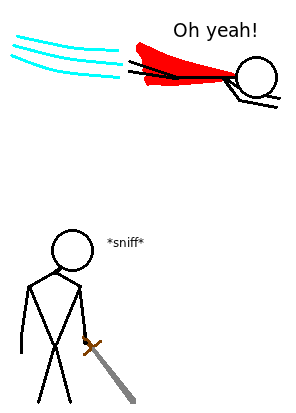
\includegraphics{Pics/Fly.png}
\end{figure*}

The subject can fly at a speed of 40 feet (or 30 feet if it wears medium or heavy armor, or if it carries a medium or heavy load). 
It can ascend at half speed and descend at double speed, and its maneuverability is good. 
Using a fly spell requires only as much concentration as walking, so the subject can attack or cast spells normally. 
The subject of a fly spell can charge but not run, and it cannot carry aloft more weight than its maximum load, plus any armor it wears.

Should the spell duration expire while the subject is still aloft, the magic fails slowly. 
The subject floats downward 60 feet per round for 1d6 rounds. 
If it reaches the ground in that amount of time, it lands safely. 
If not, it falls the rest of the distance, taking 1d6 points of damage per 10 feet of fall. 

If the spell is dispelled or negated by an \nameref{Spell:AntimagicField}, 
the subject falls like a rock, taking the appropriate falling damage.

\paragraph{Augment:} If you spend 4 additional spell points, the spell's duration increases to 1 hour per level.

When using this spell for long-distance movement, you can hustle without taking nonlethal damage 
(a forced march still requires Constitution checks). 
This means you can cover 64 miles (103 kilometres) in an eight-hour period of flight (or 48 miles (77 kilometres) at a speed of 30 feet).

\subsubsection{Fog}
\label{Spell:Fog}
Conjuration (Creation)
\\ \textbf{Level:} Air 1, Assassin 1, Conjurer, Water 1
\\ \textbf{Components:} V, S
\\ \textbf{Casting Time:} 1 standard action
\\ \textbf{Range:} 20 ft.
\\ \textbf{Effect:} Fog spreads in 20-ft. radius, 20 ft. high, centered on you
\\ \textbf{Duration:} 1 min./level
\\ \textbf{Saving Throw:} None
\\ \textbf{Spell Resistance:} No
\\ \textbf{Spell Points:} 1

\emph{A misty vapor arises around you. }

You create a bank of fog, which is stationary once created. 
The fog obscures all sight, including darkvision, beyond 5 feet. 
A creature 5 feet away has concealment (attacks have a 20\% miss chance). 
Creatures farther away have total concealment (50\% miss chance, and the attacker cannot use sight to locate the target).

A moderate wind (11+ mph), such as from a \nameref{Spell:GustOfWind} spell, disperses the fog in 4 rounds. 
A strong wind (21+ mph) disperses the fog in 1 round. 

This spell does not function underwater.

\paragraph{Augment:} You can augment the spell in one or more of the following ways:
\begin{enumerate}
 \item If you spend 2 additional spell points, the spell's duration is 10 minutes per level rather than 1 minute per level.
 \item If you spend 2 additional spell points, the spell's range increases to Medium (allowing you to create banks of fog not centered on you).
 \item If you spend 6 additional spell points, the fog becomes so thick as to be nearly solid. Anyone attempting to move through a solid fog cloud
has his speed reduced to 5 feet (assuming the speed was more than 5 feet to begin with), and takes a -2 penalty on all melee attack rolls with weapons other
than piercing weapons. The solid vapors prevent effective ranged weapon attacks (except for magic rays and the like). A creature or object that falls into
solid fog is slowed, so that each 10 feet of vapor that it passes through reduces falling damage by 1d6.
A creature can't take a 5-foot step while in solid fog.
\end{enumerate}
\subsubsection{Food and Water}
\label{Spell:FoodAndWater}
Transmutation
\\ \textbf{Level:} Water 1
\\ \textbf{Components:} V, S
\\ \textbf{Casting Time:} 1 standard action
\\ \textbf{Range:} Close (25 ft. + 5 ft./2 levels)
\\ \textbf{Target:} 1 cu. ft./level of contaminated food and water
\\ \textbf{Duration:} Instantaneous
\\ \textbf{Saving Throw:} Will negates (object)
\\ \textbf{Spell Resistance:} Yes (object)
\\ \textbf{Spell Points:} 1

\emph{Raising your hand towards the granary, you remove from the food all signs of taint.}

This spell makes spoiled, rotten, poisonous, or otherwise contaminated food and water pure and suitable for eating and drinking. 
This spell does not prevent subsequent natural decay or spoilage. 
Aligned water and similar food and drink of significance is spoiled by this spell, but the spell has no effect on creatures of any type nor upon magic potions.

\emph{Note:} Water weighs about 8 pounds per gallon. One cubic foot of water contains roughly 8 gallons and weighs about 60 pounds.

\paragraph{Augment:} If you spend 4 additional spell points, the transmutation becomes fundamentally more powerful. Instead of targeting contaminated food and water, it targets nonliving, nonmagical, unattended objects weighing up to 1 lb./level. This transforms the objects into an equivalent weight of food. Each pound of food so created is sufficient to nourish one creature for 24 hours (similar to a pound of trail rations). 
The food so created is simple - highly nourishing, if rather bland.
The food decays and becomes inedible after 24 hours, although it can be kept fresh for another 24 hours by casting another (unaugmented) instance of the spell on it.

\subsubsection{Forbiddance}
\label{Spell:Forbiddance}
Abjuration
\\ \textbf{Level:} Planes 6
\\ \textbf{Components:} V, S
\\ \textbf{Casting Time:} 6 rounds
\\ \textbf{Range:} Medium (100 ft. + 10 ft./level)
\\ \textbf{Area:} Eleven 60-ft. cubes (S)
\\ \textbf{Duration:} Permanent
\\ \textbf{Saving Throw:} See text
\\ \textbf{Spell Resistance:} Yes
\\ \textbf{Spell Points:} 11

\emph{``You are not welcome in this place!''}

Forbiddance seals an area against all planar travel into or within it. 
This includes all teleportation spells (such as \nameref{Spell:DimensionDoor} and \nameref{Spell:Teleport}), plane shifting, astral travel, ethereal travel, and all summoning spells. 
Such effects simply fail automatically.

In addition, when casting the spell, you select between one and eight alignments that the Forbiddance further wards against. You cannot select your own alignment.
Creatures of those alignments must succeed on a Will save immediately after entering a square covered by the Forbiddance or be \emph{Blown Away} in the same direction from which the creature entered.
Creatures who succeed on the saving throw can enter the area of the Forbiddance, but still experience a powerful and painful feeling of aversion.
A creature of one of the selected alignments who starts its turn in the area of the Forbiddance must make a Fortitude save or take 6d6 points of damage. This save is repeated each round for as long as the creature remains in the area\footnote{Dragging helpless creatures into a Forbiddance area that wards against it is usually considered too cruel a tactic for most Good orgnanizations to support it, unless dealing with extraordinarily Evil creatures, such as undead or Evil outsiders.}.
% In addition, it damages entering creatures whose alignments are different from yours. 
% The effect on those attempting to enter the warded area is based on their alignment relative to yours (see below). 
% A creature inside the area when the spell is cast takes no damage unless it exits the area and attempts to reenter, at which time it is affected as normal.
% 
% \begin{itemize}
% \item \emph{Alignments identical}
% No effect. The creature may enter the area freely (although not by planar travel).
% \item \emph{Alignments different with respect to either law/chaos or good/evil}
% The creature takes 6d6 points of damage. A successful Will save halves the damage, and spell resistance applies.
% \item \emph{Alignments different with respect to both law/chaos and good/evil}
% The creature takes 12d6 points of damage. A successful Will save halves the damage, and spell resistance applies.
% \end{itemize}

At your option, the abjuration can include a password, in which case creatures of the selected alignments can avoid the negative effects by speaking the password as they enter the area. 
You must select this option (and the password) at the time of casting.

\nameref{Spell:DispelMagic} cannot dispel a forbiddance effect unless the dispeller's level is at least as high as your caster level.

You can't have multiple overlapping forbiddance effects. 
In such a case, the more recent effect stops at the boundary of the older effect.

\emph{Experience Cost:} 300XP. If a password is desired, this requires an additional 200XP.

\paragraph{Augment:} For every additional spell point you spend, you can place Forbiddance upon an additional 60' cube.


\subsubsection{Foresight}
\label{Spell:Foresight}
Divination
\\ \textbf{Level:} Diviner 9, Knowledge 9
\\ \textbf{Components:} V, S
\\ \textbf{Casting Time:} 1 standard action
\\ \textbf{Range:} Personal or touch
\\ \textbf{Target:} See text
\\ \textbf{Duration:} 10 min./level
\\ \textbf{Saving Throw:} None or Will negates (harmless)
\\ \textbf{Spell Resistance:} No or Yes (harmless)
\\ \textbf{Spell Points:} 17

\emph{Suddenly, everything seems exceedingly predictable.}

This spell grants you a powerful sixth sense in relation to yourself or another. 
Once foresight is cast, you receive instantaneous warnings of impending danger or harm to the subject of the spell. 
You are never surprised or flat-footed. 
In addition, the spell gives you a general idea of what action you might take to best protect yourself,
and thus gives you a +2 insight bonus to AC and Reflex saves. 
This insight bonus is lost whenever you would lose a Dexterity bonus to AC.

When another creature is the subject of the spell, you receive warnings about that creature. 
You must communicate what you learn to the other creature for the warning to be useful, 
and the creature can be caught unprepared in the absence of such a warning. 
Shouting a warning, yanking a person back, and even telepathically communicating (via an appropriate spell) 
can all be accomplished before some danger befalls the subject, provided you act on the warning without delay. 
The subject, however, does not gain the insight bonus to AC and Reflex saves.

\subsubsection{Form of the Avian}
\label{Spell:FormAvian}
Transmutation (Polymorph)
\\ \textbf{Level:} Animal 3, Ranger 3, Transmuter 3
\\ \textbf{Components:} V,S
\\ \textbf{Casting Time:} 1 standard action
\\ \textbf{Range:} Touch
\\ \textbf{Target:} Willing living creature touched
\\ \textbf{Duration:} 10 min./level (D)
\\ \textbf{Saving Throw:} None
\\ \textbf{Spell Resistance:} No
\\ \textbf{Spell Points:} 5

\emph{The subject assumes the form of a winged bird, like that of an eagle or a swan.}

The subject undergoes the following changes:
\\ Its size changes to small.
\\ Its base strength score changes to 10.
\\ Its base dexterity score changes to 16.
\\ It gains a bite attack that deals 1d4 points of damage + your strength modifier.
This bite can be used as either a primary natural attack or a secondary natural attack.
\\ It gains the benefit of the Weapon Finesse feat.
\\ The avian form has physical wings and can fly at a speed of 60', with good maneuverability. 
\\ Its land speed changes to 10'.

However, the form has no hands, preventing the subject from using weapons and items requiring fine manipulation (although it can use its feet to hold things that can be easily gripped). It cannot provide somatic components.

\paragraph{Augment:} You can Augment this spell in one or more of the following ways:
\begin{enumerate}
 \item For every additional spell point you spend, the subject's fly speed increases by 10'.
 \item If you spend 4 additional spell points, the subject's size becomes medium when casting the spell,
 its strength score changes to 18 and its dexterity score changes to 14.
 Its bite and talon attacks (if any) have their base damage dice increased by one step.
 \item If you spend 2 additional spell points, the subject gains two talon attacks in addition to the bite
 attack. These can only be used as secondary natural attacks. The talons deal 1d3 points of
 damage + $1/2$ the subject's strength modifier. 
\end{enumerate}

\subsubsection{Form of the Dragon}
\label{Spell:FormDragon}
Transmutation (Polymorph)
\\ \textbf{Level:} Transmuter 6
\\ \textbf{Components:} V,S
\\ \textbf{Casting Time:} 1 standard action
\\ \textbf{Range:} Touch
\\ \textbf{Target:} Willing living creature touched
\\ \textbf{Duration:} 1 round/level (D)
\\ \textbf{Saving Throw:} None
\\ \textbf{Spell Resistance:} No
\\ \textbf{Spell Points:} 11

\emph{The subject assumes the form of a majestic metallic or chromatic dragon.}

The subject undergoes the following changes:
\\ Its size changes to large (long).
\\ Its base strength score changes to 26.
\\ Its base natural armor changes to 7.
\\ It gains a bite attack that deals 1d8 points of damage + its strength modifier, which is a primary natural attack.
\\ It gains two claw attacks that deal 1d6 + its strength modifier, which are secondary natural attacks.
\\ It gains two wing attacks that deal 1d4 + 1/2 its strength modifier, which are secondary natural attacks.
\\ Its land speed changes to 30'.
\\ The draconic form has physical wings and can fly at a speed of 100', with poor maneuverability.

The form is that of a quadruped, granting the subject a +4 bonus on ability checks made to resist being bull rushed or tripped when standing on the ground.
The form's front claws are capable of fine manipulation, enabling the subject to use items and provide somatic components as if it had hands.
However, the subject is not able to simultaneously walk and hold items in both front claws.

\paragraph{Augment:} You can Augment this spell in one or more of the following ways:
\begin{enumerate}
 \item For every additional spell point you spend, the strength score of the assumed form increases by 1.
 \item If you spend 4 additional spell points, the subject's size becomes huge when casting the spell, and
 its strength score changes to 28.
 The subject's bite, claw, wing and tail (if the subject has any) attacks have their base damage dice increased by one step.
 \item If you spend 4 additional spell points, the subject gains a tail attack that deals 1d8 points of damage + 
 $1 1/2$ times its strength modifier, which is a secondary natural attack.
\end{enumerate}

\subsubsection{Form of the Elemental}
\label{Spell:FormElemental}
Transmutation (Polymorph)
\\ \textbf{Level:} Air 7, Earth 7, Fire 7, Transmuter 7, Water 7.
\\ \textbf{Components:} V,S
\\ \textbf{Casting Time:} 1 standard action
\\ \textbf{Range:} Touch
\\ \textbf{Target:} Willing living creature touched
\\ \textbf{Duration:} 1 min./level (D)
\\ \textbf{Saving Throw:} None
\\ \textbf{Spell Resistance:} No
\\ \textbf{Spell Points:} 13

\emph{The subject's hair constantly moves as in a slight breeze of air.}

The subject's inner structure is radically altered, being now formed of pure elemental power. Its shape is not significantly affected.

At the time of casting, select an element. The subject gains bonuses according to the selected element.
\begin{itemize}
 \item \emph{Air Elemental:} The subject gains a fly speed of 60' (perfect maneuverability) for the duration of the spell.
 \item \emph{Earth Elemental:} The subject gains the Earth Glide ability, like a real Earth Elemental.
 \item \emph{Fire Elemental:} The subject gains immunity to fire, and vulnerability to cold.
 Those it hits with melee attacks must make a DC 15 reflex save or catch fire.
 The subject illuminates its surroundings like a torch, although it is not glaringly obvious that the subject is the source of the light.
 \item \emph{Water Elemental:} The subject gains immunity to cold, and vulnerability to fire.
 It can breathe water as well as it can breathe air, and gains a swim speed equal to its base land speed.
\end{itemize}
In addition to the qualities that depend on the selected energy type, the subject gains darkvision out to 60 feet, immunity to poison, sleep effects, paralysis, stunning, critical hits, and flanking.

% \paragraph{Augment:} If you spend 4 additional spell points, the creature is able to retain more of itself throughout the transformation.
% The creature retains all its class features when polymorphed (notably, allowing spellcasting).
% This is an exception to the general rules of Polymorph subschool spells.
\subsubsection{Form of the Fiend}
\label{Spell:FormFiend}
Transmutation (Polymorph) [Evil]
\\ \textbf{Level:} Blackguard 6, Planes 6
\\ \textbf{Components:} V,S
\\ \textbf{Casting Time:} 1 standard action
\\ \textbf{Range:} Personal
\\ \textbf{Target:} You
\\ \textbf{Duration:} 10 min./level (D)
\\ \textbf{Spell Points:} 11

\emph{You assume the form of a fiendish creature, your eyes turning black, and batlike wings sprouting from your back.}

You undergo the following changes:
\\ You grow physical wings and can fly at a speed of 100', with good maneuverability. 
\\ You gain darkvision out to 60', and low-light vision. This special darkvision allows you to see through even Magical darkness.
\\ You gain immunity to electricity and fire.
\\ You gain resistance to acid 10 and cold 10.
\\ You gain immunity to poison.
\\ You gain the telepathy special ability, out to 100 feet.
\\ Once during the spell's duration, you may use \nameref{Spell:SummonDemon} or \nameref{Spell:SummonDevil} as a spell-like ability. Caster level 9th. The casting time is as normal for the spell in question.

Your form is humanoid, with functioning hands and legs.

\paragraph{Augment:} For every additional spell point you spend, the caster level of the summoning ability increases by 1.

\subsubsection{Form of the Fish}
\label{Spell:FormFish}
Transmutation (Polymorph)
\\ \textbf{Level:} Animal 3, Ranger 3, Transmuter 3
\\ \textbf{Components:} V,S
\\ \textbf{Casting Time:} 1 standard action
\\ \textbf{Range:} Touch
\\ \textbf{Target:} Willing living creature touched
\\ \textbf{Duration:} 10 min./level (D)
\\ \textbf{Saving Throw:} None
\\ \textbf{Spell Resistance:} No
\\ \textbf{Spell Points:} 5

\emph{The subject assumes the form of a water-dwelling creature, such as a tuna or seal.}

The subject undergoes the following changes:
\\ Its size changes to small.
\\ Its base strength score changes to 14.
\\ It gains a bite attack that deals 1d6 points of damage + 1 1/2 times its strength modifier, which the subject's primary natural attack.
\\ The subject loses its land speed, and gains a swim speed of 40'.

At your option at the time of casting, the subject may gain the ability to breathe water, but lose the ability to breathe air for the duration of the spell.

Your aquatic form has no limbs that can be used to manipulate items or provide somatic components, but you may be able to hold some items (or even creatures) in your mouth, depending on your size.

\paragraph{Augment:} You can Augment this spell in one or both of the following ways:
\begin{enumerate}
 \item For every 2 additional spell points you spend, the swim speed of the form increases by 10'.
 \item For every 3 additional spell points you spend, the strength score of the form increases by 4, and it is one size category larger (to a maximum of colossal, for a 15-point additional expenditure).
 This increases the damage die of the bite attack by one step.
\end{enumerate}
\subsubsection{Form of the Horror}
\label{Spell:FormHorror}
Transmutation (Polymorph)
\\ \textbf{Level:} Blackguard 5, Transmuter 5
\\ \textbf{Components:} V,S
\\ \textbf{Casting Time:} 1 standard action
\\ \textbf{Range:} Touch
\\ \textbf{Target:} Willing living creature touched
\\ \textbf{Duration:} 1 round./level (D)
\\ \textbf{Saving Throw:} None
\\ \textbf{Spell Resistance:} No
\\ \textbf{Spell Points:} 9

\emph{The subject assumes the form of a horrific aberration, sprouting tentacles in place of arms and its skin turning into a slimy hide.}

The subject undergoes the following changes:
\\ Its base strength score changes to 18.
\\ Its base natural armor changes to 5.
\\ It gains two tentacle attacks that deal 1d8 + its strength modifier, which are primary natural attacks.
It gains the benefit of the improved grab special attack when making these tentacle attacks.
The reach of these tentacles is the same as that of a creature one size category larger than the subject's actual size.

The form functions as if one size larger than its actual size with regards to grappling (granting the appropriate size bonus on grapple checks, and allowing it to grab larger creatures).

The form has no hands, preventing the subject from using weapons and items requiring fine manipulation. It cannot provide somatic components.
However, the tentacles can be used to hold items.

\paragraph{Augment:} You can Augment this spell in one or both of the following ways:
\begin{enumerate}
 \item For every two additional spell points you spend, the subject gains an additional tentacle and tentacle attack.
 \item For every four additional spell points you spend, the effective size of the subject's form with respect to reach and grappling increases one additional category above its own.
\end{enumerate}
\subsubsection{Form of the Iron Golem}
\label{Spell:FormIronGolem}
Transmutation (Polymorph)
\\ \textbf{Level:} Earth 8, Transmuter 8
\\ \textbf{Components:} V,S
\\ \textbf{Casting Time:} 1 standard action
\\ \textbf{Range:} Touch
\\ \textbf{Target:} Willing living creature touched
\\ \textbf{Duration:} 1 minute./level (D)
\\ \textbf{Saving Throw:} None
\\ \textbf{Spell Resistance:} No
\\ \textbf{Spell Points:} 15

\emph{This spell transforms the subject's body into living iron.}

The subject undergoes the following changes:
\\ It gains damage reduction 15/adamantine. 
\\ It gains immunity to blindness, critical hits, ability score damage, deafness, disease, drowning, electricity, poison, stunning, and all spells or attacks that affect its physiology or respiration, because it has no physiology or respiration while this spell is in effect.
\\ It becomes vulnerable to the Rusting Grasp spell and rust monsters. 
\\ Its size changes to large (tall).
\\ Its base strength score changes to 30.
\\ Its base dexterity score changes to 6.
\\ Its base natural armor changes to 8.
\\ It gains a slam attack that deals 1d10 + 1 1/2 times its strength modifier, which is a primary natural attack.
\\ The subject's land speed changes to 20'.

The subject cannot drink (and thus can't use potions) or play wind instruments. 
Its weight increases by a factor of ten, causing it to sink in water like a stone (the subject loses any swim speed it may have, and it automatically fails all swim checks).
However, it could survive the crushing pressure and lack of air at the bottom of the ocean - at least until the spell duration expires.

\paragraph{Augment:} You can Augment this spell in one or more of the following ways:
\begin{enumerate}
 \item For every additional spell point you spend, the strength score of the assumed form increases by 2.
 \item For every additional spell point you spend, the damage reduction offered by this spell increases by 2.
\end{enumerate}
\subsubsection{Form of the Plant}
\label{Spell:FormPlant}
Transmutation (Polymorph)
\\ \textbf{Level:} Plant 2
\\ \textbf{Components:} V,S
\\ \textbf{Casting Time:} 1 standard action
\\ \textbf{Range:} Personal
\\ \textbf{Target:} You
\\ \textbf{Duration:} 1 hour/level (D)
\\ \textbf{Spell Points:} 3

\emph{You assume the form of a tree, bush, a vine or other kind of appropriately sized plant.}

You undergo the following changes:
\\ Your size changes to large (tall), large (long), or medium, chosen at the time of casting.
\\ You lose your strength and dexterity scores (they change to ``-``), becoming immobile.
\\ You gain immunity to poison, sleep effects, paralysis, stunning, and critical hits.
\\ You lose your ability to see and hear, but you gain the Blindsense ability out to 60'.

You become rooted when on the ground, granting you a +20 bonus on ability checks made to resist being bull rushed or tripped when standing on the ground. Your climb DC is 10.
Use the maximum carrying capacity of your unpolymorphed form to determine whether the the plant can support the climber's weight.

You gain a +16 racial bonus on hide checks when in forested areas, and a +30 bonus on Disguise checks made to pretend being a tree.

\paragraph{Augment:} You can Augment this spell in one of the following ways:
\begin{enumerate}
 \item If you spend 2 additional spell points, you can choose to become a small or tiny plant.
 \item If you spend 6 additional spell points, you can choose to become a diminutive or fine plant.
 \item If you spend 4 additional spell points, you can choose to become a huge plant.
 \item If you spend 6 additional spell points, you can choose to become a gargantuan plant.
 \item If you spend 8 additional spell points, you can choose to become a colossal plant.
\end{enumerate}
\subsubsection{Form of the Predator}
\label{Spell:FormCarnivore}
Transmutation (Polymorph)
\\ \textbf{Level:} Animal 4, Ranger 4, Transmuter 4
\\ \textbf{Components:} V,S
\\ \textbf{Casting Time:} 1 standard action
\\ \textbf{Range:} Touch
\\ \textbf{Target:} Willing living creature touched
\\ \textbf{Duration:} 1 round/level (D)
\\ \textbf{Saving Throw:} None
\\ \textbf{Spell Resistance:} No
\\ \textbf{Spell Points:} 7

\emph{The subject assumes the form of a large, dangerous beast, like a tiger or a bear.}

The subject undergoes the following changes:
\\ Its size changes to large (long).
\\ Its base strength score changes to 22.
\\ Its base natural armor changes to 5.
\\ It gains two claw attacks that deal 1d8 + its strength modifier, which are primary natural attacks.
\\ It gains a bite attack that deals 2d6 points of damage + $1/2$ its strength modifier, which is a secondary natural attack.
\\ Its land speed changes to 40'.

Its form is that of a quadruped, granting it a +4 bonus on ability checks made to resist being bull
rushed or tripped when standing on the ground. 
However, the form has no hands, preventing the subject from using weapons and items requiring fine manipulation (although it can use its feet to hold things that can be easily gripped). It cannot provide somatic components.

\paragraph{Augment:} You can Augment this spell in one or more of the following ways:
\begin{enumerate}
 \item For every two additional spell points you spend, the strength score of the assumed form increases by 3.
 \item If you spend 6 additional spell points, the subject's size becomes huge when casting the spell, and its strength score changes to 28.
 The bite and claw attacks have their base damage dice increased by one step.
 \item If you spend 12 additional spell points, the subjects' size becomes gargantuan when casting the spell, and its strength score changes to 34.
 The bite and claw attacks have their base damage dice increased by two steps.
 \item For every two additional spell points you spend, the base natural armor of the assumed form increases by 1.
\end{enumerate}
\subsubsection{Form of the Scout}
\label{Spell:FormScout}
Transmutation (Polymorph)
\\ \textbf{Level:} Transmuter 2
\\ \textbf{Components:} V,S
\\ \textbf{Casting Time:} 1 standard action
\\ \textbf{Range:} Touch
\\ \textbf{Target:} Willing living creature touched
\\ \textbf{Duration:} 10 min./level (D)
\\ \textbf{Saving Throw:} None
\\ \textbf{Spell Resistance:} No
\\ \textbf{Spell Points:} 3

\emph{The subject assumes the form of a fast, agile creature.}

The subject undergoes the following changes:
\\ Its size changes to tiny.
\\ Its base strength score changes to 2.
\\ Its base dexterity score changes to 14.
\\ Its land speed changes to 30'.
\\ It gains no natural attacks.

The form is that of a quadruped, granting the subject a +4 bonus on ability checks made to resist being bull rushed or tripped when standing on the ground.
The form has no hands, preventing the subject from using weapons and items requiring fine manipulation. It cannot provide somatic components.
It may be able to use its mouth to hold items, within the limits of its new strength score.

As a tiny creature, the subject has a +8 size bonus on hide checks. It also gains a complimentary +8 racial bonus on move silently checks.

At the time of casting, you choose one enhanced mode of movement from the following list, which the subject gains:
\begin{itemize}
 \item A burrow speed of 20'.
 \item A climb speed of 20'.
 \item A swim speed of 20'.
 \item An increase in base land speed, up to 50'.
\end{itemize}

\paragraph{Augment:} You can Augment this spell in one or two of the following ways:
\begin{enumerate}
 \item For every 2 additional spell points you spend, the burrow, climb, swim, or land speed increases by 10'.
 The mode of movement so augmented is the same as the one you chose to enhance at the time of casting.
 \item If you spend 4 additional spell points, the subject's size decreases to diminutive, its base strength score changes to 1, and its base dexterity score changes to 16. The racial bonus on move silently checks increases to +12, and as a diminutive creature, the subject has a +12 size bonus on hide checks.
 \item If you spend 12 additional spell points, the subject's size decreases to fine, its base strength score changes to 1, and its base dexterity score changes to 20. The racial bonus on move silently checks increases to +16, and as a fine creature, the subject has a +16 size bonus on hide checks.
\end{enumerate}
\subsubsection{Form of the Titan}
\label{Spell:FormTitan}
Transmutation (Polymorph)
\\ \textbf{Level:} Strength 9
\\ \textbf{Components:} V,S
\\ \textbf{Casting Time:} 1 standard action
\\ \textbf{Range:} Touch
\\ \textbf{Target:} Willing living creature touched
\\ \textbf{Duration:} 1 round/level (D)
\\ \textbf{Saving Throw:} None
\\ \textbf{Spell Resistance:} No
\\ \textbf{Spell Points:} 17

\emph{The subject assumes the form of an enormous giant with bulging muscles.}

The subject undergoes the following changes:
\\ Its size changes to Huge.
\\ Its base strength score changes to 43.
\\ Its base natural armor changes to 19.
\\ It gains two slam attacks that deal 1d8 + its strength modifier, which are secondary natural attacks.
\\ It can use \nameref{Spell:ChainLightning} as a spell-like ability. Its save DC is charisma-based, and its caster level is equal to the subject's hit die.
\\ Its land speed changes to 60'.

Any weapon the subject may wield is magically resized to huge, and bypasses damage reduction as if it were made of adamantine.
The subject's body shape is mostly unchanged.

\paragraph{Augment:} For every additional spell point you spend, the subject's strength score increases by 2, and its natural armor increases by 1.
\subsubsection{Form of the Treant}
\label{Spell:FormTreant}
Transmutation (Polymorph)
\\ \textbf{Level:} Plant 5, Ranger 5, Transmuter 5
\\ \textbf{Components:} V,S
\\ \textbf{Casting Time:} 1 standard action
\\ \textbf{Range:} Touch
\\ \textbf{Target:} Willing living creature touched
\\ \textbf{Duration:} 1 round/level (D)
\\ \textbf{Saving Throw:} None
\\ \textbf{Spell Resistance:} No
\\ \textbf{Spell Points:} 9

\emph{The subject assumes the form of a mobile plant creature.}

The subject undergoes the following changes:
\\ Its size changes to large (tall).
\\ Its base strength score changes to 22.
\\ Its base natural armor changes to 9, and it gains damage reduction 10/slashing.
\\ It gains a slam attack that deals 1d8 points of damage + $1 1/2$ times its strength modifier, which is a primary natural attack.
\\ It gains the trample special attack, which follows the normal rules for such attacks.
\\ It gains immunity to poison, sleep effects, paralysis, stunning, and critical hits.
\\ Its land speed changes to 20'.

The form is partially rooted when on the ground, granting the subject a +10 bonus on ability checks made to resist being bull
rushed or tripped when standing on the ground.

The form has no hands, preventing the subject from using weapons and items requiring fine manipulation. It cannot provide somatic components.
However, the subject can bend its appendages to pick up objects.

The subject gains a +16 racial bonus on hide checks when in forested areas, and a +16 bonus on Disguise checks made to pretend being a tree.

\paragraph{Augment:} You can Augment this spell in one or more of the following ways:
\begin{enumerate}
 \item For every additional spell point you spend, the natural armor of the assumed form increases by 1.
 \item If you spend 4 additional spell points, the subject's size becomes huge when casting the spell, and its strength score changes to 26.
 The slam attack has its base damage die increased by one step.
 \item If you spend 8 additional spell points, the subject's size becomes gargantuan when casting the spell, and its strength score changes to 30.
 The slam attack has its base damage die increased by two steps.
\end{enumerate}
\subsubsection{Form of the Vermin}
\label{Spell:FormVermin}
Transmutation (Polymorph)
\\ \textbf{Level:} Transmuter 4, Vermin 4
\\ \textbf{Components:} V,S
\\ \textbf{Casting Time:} 1 standard action
\\ \textbf{Range:} Touch
\\ \textbf{Target:} Willing living creature touched
\\ \textbf{Duration:} 1 min./level (D)
\\ \textbf{Saving Throw:} None; see text
\\ \textbf{Spell Resistance:} No
\\ \textbf{Spell Points:} 7

\emph{The subject assumes the form of a gigantic insect, arachnid, crustacean or other generally repugnant creature.}

The subject undergoes the following changes:
\\ Its size changes to medium.
\\ Its base strength score changes to 18.
\\ It gains a sting attack that deals 2d6 points of damage + $1 1/2$ times its strength modifier, which is a primary natural attack.
The stinger is poisonous, dealing 1d6 points of primary and secondary dexterity damage. The poison's save DC is equal to this spell's save DC.
If the spell ends, all poison the subject has secreted immediately disappears, including poison that has been injected into a creature but has yet to deal its secondary damage. 
However, any damage the poison may already have inflicted remains.
Using this poison against a sapient creature (intelligence score of 3 or above) is an evil act.
\\Its land speed changes to 40'.

The form has multiple pairs of legs, granting the subject a +4 bonus on ability checks made to resist being bull rushed or tripped when standing on the ground. 
It gains a climb, swim or burrow speed of 20', chosen at the time of casting.

The form has no hands, preventing the subject from using weapons and items requiring fine manipulation. It cannot provide somatic components.

\paragraph{Augment:} You can Augment this spell in one or more of the following ways:
\begin{enumerate}
 \item If you spend 2 additional spell points, the subject's size becomes large (long) when casting the spell, and its strength score changes to 20.
 The sting attack (and claw or slam attacks, if you have them) has its base damage die increased by one step.
 \item If you spend 6 additional spell points, the subject's size becomes huge when casting the spell, and its strength score changes to 24.
 The sting attack (and claw or slam attacks, if you have them) has its base damage die increased by two steps. 
 The poison's primary and secondary dexterity damage increases to 1d8.
 \item If you spend 2 additional spell points, the subject gains two slam or claw attacks (your choice).
 These secondary attacks deal 1d6 points of damage + $1/2$ the subject's strength modifier.
 \item For every additional spell point you spend, the stinger's poison save DC increases by 1 above and beyond that normally offered by a spell of this power.
\end{enumerate}
\subsubsection{Form of the Viper}
\label{Spell:FormViper}
Transmutation (Polymorph)
\\ \textbf{Level:} Transmuter 4, Vermin 4
\\ \textbf{Components:} V,S
\\ \textbf{Casting Time:} 1 standard action
\\ \textbf{Range:} Touch
\\ \textbf{Target:} Willing living creature touched
\\ \textbf{Duration:} 1 min./level (D)
\\ \textbf{Saving Throw:} None; see text
\\ \textbf{Spell Resistance:} No
\\ \textbf{Spell Points:} 7

\emph{The subject assumes the form of a dangerous snake.}

The subject undergoes the following changes:
\\ Its size changes to large (long).
\\ Its base strength score changes to 20.
\\ It gains a bite attack that deals 1d8 points of damage + $1 1/2$ times its strength modifier, which is a primary natural attack.
The bite is poisonous, dealing 1d6 points of primary and secondary constitution damage. The poison's save DC is equal to this spell's save DC.
If the spell ends, all poison the subject has secreted immediately disappears, including poison that has been injected into a creature, but has yet to deal its secondary damage. However, any damage the poison may already have inflicted remains.
Using this poison against a sapient creature (intelligence score of 3 or above) is an evil act.
\\ The subject gains the constrict special attack. It deals damage equal to the damage dealt by the bite attack, except the constriction damage is bludgeoning damage, and does not deliver poison.
The subject does not provoke an attack of opportunity when starting a grapple as if it had the Improved Grapple feat.
\\ Its land speed changes to 20'.

The form has no legs, granting the subject immunity to trip attacks, and a +4 bonus on ability checks made to resist being bull rushed when standing on the ground.

The viper form has no limbs that can be used to manipulate items, but the subject may be able to hold some items in its mouth, depending on the form's size.
\paragraph{Augment:} You can Augment this spell in one or more of the following ways:
\begin{enumerate}
 \item If you spend 6 additional spell points, the subject's size becomes huge when casting the spell, and its strength score changes to 24.
 The bite attack has its base damage die increased by one step.
 \item If you spend 12 additional spell points, the subject's size becomes gargantuan when casting the spell, and its strength score changes to 30.
 The bite attack has its base damage die increased by two steps.
 \item For every additional spell point you spend, the bite's poison save DC increases by 1 above and beyond that
 normally offered by a spell of this power.
\end{enumerate}

\subsubsection{Fortune of the Gods}
\label{Spell:FortuneOfTheGods}
Evocation
\\ \textbf{Level:} Luck 9
\\ \textbf{Components:} V, S
\\ \textbf{Casting Time:} 1 standard action
\\ \textbf{Range:} Personal
\\ \textbf{Target:} You
\\ \textbf{Duration:} 1 round/level
\\ \textbf{Spell Points:} 17

\emph{Your divine patron smiles upon you, subtly twisting all circumstances slightly in your favor.}

For the duration of the spell, whenever you make a d20 roll, roll two dice and choose the result you prefer. Any ability that allows you to reroll a die only affects one of the dice you roll.

\subsubsection{Freedom}
\label{Spell:Freedom}
Abjuration
\\ \textbf{Level:} Sor/Wiz 9
\\ \textbf{Components:} V, S
\\ \textbf{Casting Time:} 1 standard action
\\ \textbf{Range:} Close (25 ft. + 5 ft./2 levels) or see text
\\ \textbf{Target:} One creature
\\ \textbf{Duration:} Instantaneous, then 1 round/level; see text
\\ \textbf{Saving Throw:} Will negates (harmless)
\\ \textbf{Spell Resistance:} Yes
\\ \textbf{Spell Points:} 17

\emph{Freedom is not a spell. It is an idea.}

The subject is freed from the effect of a \nameref{Spell:Binding}, \nameref{Spell:Imprisonment}, \nameref{Spell:Maze} and/or a \nameref{Spell:TemporalStasis} spell.

To free a creature from imprisonment or \nameref{Spell:Maze}, 
you must know its name and background, and you must cast this spell at the spot where it was entombed or banished into the maze.

The freedom effect itself is instantaneous. 
But in addition, the subject of the Freedom spell gains the benefits of the \nameref{Spell:FreedomOfMovement} after the Freedom spell has been cast,
except for that the duration of the Freedom of Movement is 1 round per level.
It is possible to cast the Freedom spell on a creature that isn't imprisoned simply to give it this secondary benefit.

\paragraph{Augment:} For every 2 additional spell points you spend, this spell can target an additional creature within range.

\subsubsection{Free Step}
\label{Spell:FreeStep}
Conjuration (Teleportation)
\\ \textbf{Level:} Planes 1, Travel 1
\\ \textbf{Components:} V
\\ \textbf{Casting Time:} 1 swift action
\\ \textbf{Range:} 10 feet
\\ \textbf{Target:} You
\\ \textbf{Duration:} Instantaneous
\\ \textbf{Spell Points:} 1

\emph{A quick step through the astral plane is useful for getting around.}

You instantly teleport yourself to an unoccupied space within the spell's range.
You must have line of sight and line of effect to the destination.

\paragraph{Augment:} For every additional spell point you spend, the spell's range increases by 5 feet.

\subsubsection{Freedom of Movement}
\label{Spell:FreedomOfMovement}
Abjuration
\\ \textbf{Level:} Bard 4, Blackguard 4, Luck 4, Ranger 4, Travel 4
\\ \textbf{Components:} V, S
\\ \textbf{Casting Time:} 1 standard action
\\ \textbf{Range:} Personal or touch
\\ \textbf{Target:} You or creature touched
\\ \textbf{Duration:} 10 min./level or until discharged; see text
\\ \textbf{Saving Throw:} Will negates (harmless)
\\ \textbf{Spell Resistance:} Yes (harmless)
\\ \textbf{Spell Points:} 7

\emph{There is no holding you back now.}

This spell enables the subject to move and attack normally for the duration of the spell, even under the influence of certain magic and conditions that usually impede movement.
\begin{itemize}
 \item The subject gains immunity to the conditions of being \emph{Entangled}, \emph{Immobilized} and \emph{Paralyzed}.
 \item The subject gains immunity to the effects of the spells \nameref{Spell:Entangle}, \nameref{Spell:Fog} (immunity to the movement-hampering effects of its third augment only. The subject does not gain the ability to see through the fog.), \nameref{Spell:Grease}, \nameref{Spell:Slow} and \nameref{Spell:Web} (the webs still provide cover and such, the subject simply gains the ability to walk through the spell's area unhindered).
\end{itemize}
Note that the subject may be further immune to the effects of some spells (such as the \nameref{Spell:HoldPerson} spell) due to it being immune to the condition that the spell inflicts.

The spell also allows the subject to move and attack normally while underwater, even with slashing weapons such as axes and swords or with bludgeoning weapons such as flails, hammers, and maces, provided that the weapon is wielded in the hand rather than hurled. The freedom of movement spell does not, however, allow water breathing.

At any point during the spell's duration, the subject may discharge it as an immediate action to automatically succeed on any grapple check made to resist a grapple attempt, as well as on grapple checks or Escape Artist checks made to escape a grapple or a pin made within 1 round of the discharge. 

\paragraph{Augment:} If you spend 6 additional spell points, the subject automatically succeeds on the outlined grapple and Escape Artist checks for 1 round/level after discharging the spell, rather than for 1 round.
\subsubsection{Freezing Sphere}
\label{Spell:FreezingSphere}
Evocation [Cold]
\\ \textbf{Level:} Sor/Wiz 6
\\ \textbf{Components:} S
\\ \textbf{Casting Time:} 1 standard action
\\ \textbf{Range:} Long (400 ft. + 40 ft./level)
\\ \textbf{Area:} 10-foot-radius burst; see text
\\ \textbf{Duration:} 1 round/level; see text
\\ \textbf{Saving Throw:} Reflex partial; see text
\\ \textbf{Spell Resistance:} Yes
\\ \textbf{Spell Points:} 11

\emph{You creates a frigid globe of cold energy that streaks from your fingertips to the location you select, where it silently pulses out.} 

Each creature in the area takes 6d6 points of cold damage. 
An elemental (water) creature instead takes 12d6 points of cold damage.
In addition, all creatures within the bursts are frozen in place, \emph{immobilized}.
The creatures remain \emph{immobilized} for 1 round/level unless they succeed on a Reflex save (which reduces the duration as far as that creature is concerned to 1 round).
An \emph{immobilized} creature may attempt a DC 25 Strength check or a DC 25 Escape Artist check to escape as a full round action.

If the freezing sphere strikes a body of water or a liquid that is principally water (not including water-based creatures), the radius of the spell increases to 100' (but never beyond the edge of the body of water, unless the edge is within the spell's normal 10' radius).
This freezes the liquid over to a depth of 6 inches for 1 round per level.

\paragraph{Augment:} For every additional spell point you spend, this spell deals an additional 1d6 points of damage to elemental (water) creatures.
In addition, for every 2 additional spell points you spend, the damage against other creatures increases by 1d6.
\subsection{'G' Spells}
\subsubsection{Gaseous Form}
\label{Spell:GaseousForm}
Transmutation
\\ \textbf{Level:} Air 3, Assassin 3, Bard 3, Sor/Wiz 3
\\ \textbf{Components:} V, S
\\ \textbf{Casting Time:} 1 standard action
\\ \textbf{Range:} Touch
\\ \textbf{Target:} Willing corporeal creature touched
\\ \textbf{Duration:} 1 min./level (D)
\\ \textbf{Saving Throw:} None
\\ \textbf{Spell Resistance:} No
\\ \textbf{Spell Points:} 5

\emph{You melt into mist.}

The subject and all its gear become insubstantial, misty, and translucent. 
Its material armor (including natural armor) becomes worthless, though its size, 
Dexterity, deflection bonuses, and armor bonuses from force effects still apply. 
The subject gains damage reduction 10/magic and becomes immune to poison and critical hits. 
It can't attack or provide verbal or somatic components while in gaseous form. 
The subject also loses supernatural abilities while in gaseous form. 
If it has a touch spell ready to use, that spell is discharged harmlessly when the gaseous form spell takes effect.

A gaseous creature can't run, but it can fly at a speed of 10 feet (maneuverability perfect). 
It can pass through small holes or narrow openings, even mere cracks, 
with all it was wearing or holding in its hands, as long as the spell persists. 
The creature is subject to the effects of wind, and it can't enter water or other liquid. 
It also can't manipulate objects or activate items, even those carried along with its gaseous form. 
Continuously active items remain active, though in some cases their effects may be moot.

The subject of the spell can will itself to resume corporeal form as a standard action,

\paragraph{Augment:} You can Augment this spell in one or both of the following ways:
\begin{enumerate}
 \item If you spend four additional spell points, the subject can evoke a powerful wind to increase its speed while in gaseous form.
 At the start of every round of the spell's duration, it can decide whether the wind is active or not. If it decides that it is,
 its fly speed increases to 600 feet, but its maneuverability drops to clumsy. In rounds when the wind is not active,
 the fly speed is unchanged.
 \item If you spend two additional spell points, the spell's duration increases to 1 hour per level.
\end{enumerate}
\subsubsection{Gate}
\label{Spell:Gate}
Conjuration (Creation or Calling) [see text]
\\ \textbf{Level:} Conjurer 9, Planes 9
\\ \textbf{Components:}  V, S
\\ \textbf{Casting Time:} 1 standard action
\\ \textbf{Range:} Medium (100 ft. + 10 ft./level)
\\ \textbf{Effect:} See text
\\ \textbf{Duration:} Instantaneous or concentration (up to 1 round/level); see text
\\ \textbf{Saving Throw:} None
\\ \textbf{Spell Resistance:}  No
\\ \textbf{Spell points:} 17

\emph{With a flash of light, reality folds in on itself and connects two places across the planes.}

Casting a gate spell has two effects. 
First, it creates an interdimensional connection between your plane of existence and a plane you specify, allowing travel between those two planes in either direction.

Second, you may then call a particular individual or kind of being through the gate.

The gate itself is a circular hoop or disk from 5 to 20 feet in diameter (caster's choice), 
oriented in the direction you desire when it comes into existence (typically vertical and facing you). It is a two-dimensional window looking into the plane you specified when casting the spell, and anyone or anything that moves through is shunted instantly to the other side.

A gate has a front and a back. Creatures moving through the gate from the front are transported to the other plane; creatures moving through it from the back are not.
\begin{itemize}
\item \emph{Planar Travel:}

As a mode of planar travel, a gate spell functions much like a \nameref{Spell:PlaneShift} spell, 
except that the gate opens precisely at the point you desire (a creation effect). 
Deities and other beings who rule a planar realm can prevent a gate from opening in their presence or personal demesnes if they so desire. 
Travelers need not join hands with you-anyone who chooses to step through the portal is transported. 
A gate cannot be opened to another point on the same plane; the spell works only for interplanar travel.

You may hold the gate open only for a brief time (no more than 1 round per caster level), 
and you must concentrate on doing so, or else the interplanar connection is severed.
\item \emph{Calling Creatures:}

The second effect of the gate spell is to call an extraplanar creature to your aid (a calling effect). 
By naming a particular being or kind of being as you cast the spell, 
you cause the gate to open in the immediate vicinity of the desired creature and pull the subject through, 
willing or unwilling. Deities and unique beings are under no compulsion to come through the gate, although they may choose to do so of their own accord. 
This use of the spell creates a gate that remains open just long enough to transport the called creatures. This use of the spell has an XP cost (see below).

If you choose to call a kind of creature instead of a known individual you may call either a single creature or several creatures, whose total HD is no more than 20.
The creature or creatures you call are not under your control, but diplomacy, intimidation, and negotiation work as normal. 
If called into the middle of a fight, a creature usually acts according to its type or alignment
(for example, most angels will not pass up the chance to fight a demon), but its allegiance to you is not assured.

At the end of the spell's duration, the creature is sent back to the place it came from.
% If you choose to call a kind of creature instead of a known individual you may call either a single creature (of any HD) or several creatures. 
% You can call and control several creatures as long as their HD total does not exceed your caster level. 
% In the case of a single creature, you can control it if its HD do not exceed twice your caster level. 
% A single creature with more HD than twice your caster level can't be controlled. 
% Deities and unique beings cannot be controlled in any event. 
% An uncontrolled being acts as it pleases, making the calling of such creatures rather dangerous. 
% An uncontrolled being may return to its home plane at any time.
% 
% A controlled creature can be commanded to perform a service for you. 
% Such services fall into two categories: immediate tasks and contractual service. 
% Fighting for you in a single battle or taking any other actions that can be accomplished within 1 round per caster level counts as an immediate task; 
% you need not make any agreement or pay any reward for the creature's help. The creature departs at the end of the spell.
% 
% If you choose to exact a longer or more involved form of service from a called creature, you must offer some fair trade in return for that service. 
% The service exacted must be reasonable with respect to the promised favor or reward; see the lesser planar ally spell for appropriate rewards. 
% (Some creatures may want their payment in ``livestock`` rather than in coin, which could involve complications.) 
% Immediately upon completion of the service, the being is transported to your vicinity, 
% and you must then and there turn over the promised reward. After this is done, the creature is instantly freed to return to its own plane.
% 
% Failure to fulfill the promise to the letter results in your being subjected to service by the creature or by its liege and master, at the very least. 
% At worst, the creature or its kin may attack you.

Note: When you use a calling spell such as gate to call an air, chaotic, earth, evil, fire, good, lawful, or water creature, it becomes a spell of that type.
\end{itemize}

\paragraph{Augment:} For every additional spell point you spend, 
the spell's calling creatures function can call in creatures whose HD total is one higher when calling a type of creature.

\emph{Experience cost:} 1,000 XP (only for the calling creatures function). 
\subsubsection{Geas (Quest)}
\label{Spell:GeasQuest}
Enchantment (Compulsion) [Language-Dependent, Mind-Affecting]
\\ \textbf{Level:} Bard 3, Blackguard 3, Enchanter 4, Law 4, Paladin 3
\\ \textbf{Components:} V
\\ \textbf{Casting Time:} 1 round
\\ \textbf{Range:} Close (25 ft. + 5 ft./2 levels)
\\ \textbf{Target:} One living creature with 7 HD or less
\\ \textbf{Duration:} Permanent until discharged; see text
\\ \textbf{Saving Throw:} Will negates
\\ \textbf{Spell Resistance:} Yes
\\ \textbf{Spell Points:} Bard 5, Enchanter 7, Law 7, Paladin 5

\emph{''Go now. Return successfully, or not at all.``}

A geas places a magical command on a creature to carry out some service or to refrain from some action or course of activity, 
as desired by you. The creature must have 7 or fewer Hit Dice and be able to understand you. 
While a geas cannot compel a creature to kill itself or perform acts that would result in certain death, 
it can cause almost any other course of activity.

The geased creature must follow the given instructions until the geas is completed, no matter how long it takes.

If the instructions involve some open-ended task that the recipient cannot complete through his own actions the spell 
remains in effect for a maximum of one day per caster level. A clever recipient can subvert some instructions.

If the subject is prevented from obeying the lesser geas for 24 hours, 
it takes a -2 penalty to each of its ability scores. 
Each day, another -2 penalty accumulates, up to a total of -8. 
No ability score can be reduced to less than 1 by this effect. 
The ability score penalties are removed 24 hours after the subject resumes obeying the geas.

A geas (and all ability score penalties) can not be dispelled, but it can be removed by any effect that would remove a \nameref{sec:Curses} (See: \nameref{sec:RemovingACurse}).

Clerics and Paladins usually refer to this spell as \emph{Quest} rather than geas.

\paragraph{Augment:} For every additional spell point you spend, this spell's hit dice cap increases by 1.

\subsubsection{Gelugon's Spear}
\label{Spell:GelugonsSpear}
Transmutation [Evil]
\\ \textbf{Level:} Blackguard 3
\\ \textbf{Components:} V, S
\\ \textbf{Casting Time:} 1 standard action
\\ \textbf{Range:} Touch
\\ \textbf{Target:} Melee weapon touched
\\ \textbf{Duration:} 1 round/level
\\ \textbf{Saving Throw:} None; see text
\\ \textbf{Spell Resistance:} No; see text
\\ \textbf{Spell Points:} 5

\emph{Your weapon gains a frost coating that emits cold fumes, like that of an ice devil.}

A creature struck by a weapon imbued with this spell must make a Fortitude save or be slowed for 1d6 rounds.
This effect is subject to spell resistance.

\subsubsection{Genesis}
\label{Spell:Genesis}
Conjuration (Creation)
\\ \textbf{Level:} Sor/Wiz 9
\\ \textbf{Components:} V
\\ \textbf{Casting Time:} One week (8 hours/day)
\\ \textbf{Range:} 180 ft.; see text
\\ \textbf{Effect:} A demiplane coterminous with the Astral Plane, centered on your location
\\ \textbf{Duration:} Instantaneous
\\ \textbf{Saving Throw:} None
\\ \textbf{Spell Resistance:} No
\\ \textbf{Spell Points:} 17, XP

\emph{As you begin casting the spell, you can't help but wonder if this shouldn't qualify you for godhood.}

You create a finite plane with limited access: a demiplane. 
Demiplanes created by this spell are very small, very minor planes. 
This spell works only when cast while you are on the Astral Plane. 
The casting of this spell creates a local density fluctuation that precipitates the creation of a demiplane. 
The fledgling plane grows in radius at a rate of 1 foot per day to an initial maximum radius of 180 feet as it rapidly draws substance from the surrounding astral ectoplasm. 
%Once the new demiplane reaches its maximum size, it doesn't really stop growing, but its growth rate decreases to only 1 foot per week (approximately a 50-foot increase in radius per year).
Once your demiplane is created, you can travel to it using \nameref{Spell:PlaneShift}, \nameref{Spell:Gate} or some other spell or permanent link that you arrange for separately.

You determine the environment within the demiplane when you cast genesis, reflecting most any desire you can visualize. 
You determine factors such as atmosphere, water, temperature, and the general shape of the terrain. 
This spell cannot create life (including vegetation), nor can it create construction (such as buildings, roads, wells, dungeons, and so forth). 
You must add these details in some other fashion if you desire. 
You can't create lingering magical effects with this spell; you have to add those separately, if desired. 
Similarly, you can't create a demiplane out of esoteric material, such as silver or uranium; you're limited to stone and dirt. 

You can't manipulate the time trait on your demiplane; its time trait is as the Material Plane.
Its size trait is determined by the limitations of this spell.
If you have a divine rank of 1 or higher, you can select any Morphic Traits, otherwise you are limited to creating alterable morphic planes.

Once your demiplane reaches 180 feet in radius, you can cast this spell again to gradually add another 180 feet of radius to it, and so on.

\emph{Experience Cost:} 1,000 XP. 
\subsubsection{Gentle Repose}
\label{Spell:GentleRepose}
Necromancy
\\ \textbf{Level:} Death 2, Healing 2, Necromancer 2
\\ \textbf{Components:} V, S
\\ \textbf{Casting Time:} 1 standard action
\\ \textbf{Range:} Touch
\\ \textbf{Target:} Corpse touched
\\ \textbf{Duration:} One day/level
\\ \textbf{Saving Throw:} Will negates (object)
\\ \textbf{Spell Resistance:} Yes (object)
\\ \textbf{Spell Points:} 3

\emph{''Nothing shall touch these remains.``}

You preserve the remains of a dead creature so that they do not decay. 
Doing so effectively extends the time limit on raising that creature from the dead (see \nameref{Spell:RaiseDead}). 
Days spent under the influence of this spell don't count against the time limit. 
Additionally, this spell makes transporting a fallen comrade more pleasant.

The spell also works on severed body parts and the like.

\paragraph{Augment:} For every 2 additional spell points you touch, this spell can affect an additional corpse.

\subsubsection{Ghoul Touch}
\label{Spell:GhoulTouch}
Necromancy
\\ \textbf{Level:} Blackguard 2, Sor/Wiz 2
\\ \textbf{Components:} V, S
\\ \textbf{Casting Time:} 1 standard action
\\ \textbf{Range:} Touch
\\ \textbf{Target:} Living humanoid touched
\\ \textbf{Duration:} 1d6+2 rounds
\\ \textbf{Saving Throw:} Fortitude negates
\\ \textbf{Spell Resistance:} Yes
\\ \textbf{Spell Points:} 3

\emph{The stink of death momentarily fills the air.}

Imbuing yourself with negative energy, this spell allows you to \emph{paralyze} a single living humanoid for the duration of the spell with a successful melee touch attack.

Additionally, the paralyzed subject exudes a carrion stench that causes all living creatures (except you) in a 10-foot-radius spread to become sickened (Fortitude negates). 

An \nameref{Spell:Antipoison} spell removes the effect from a sickened creature, and creatures immune to poison are unaffected by the stench.

Elves are immune to this spell.

\paragraph{Augment:} If you spend 4 additional spell points, those that would become sickened by the stench instead become nauseated.

\subsubsection{Giant Vermin}
\label{Spell:GiantVermin}
Transmutation
\\ \textbf{Level:} Vermin 4
\\ \textbf{Components:} V, S
\\ \textbf{Casting Time:} 1 standard action
\\ \textbf{Range:} Close (25 ft. + 5 ft./2 levels)
\\ \textbf{Targets:} Up to three vermin, no two of which can be more than 30 ft. apart
\\ \textbf{Duration:} 1 min./level
\\ \textbf{Saving Throw:} None
\\ \textbf{Spell Resistance:} Yes
\\ \textbf{Spell Points:} 7

\emph{The vermin inflate like grotesque balloons.}

You turn three normal-sized centipedes, two normal-sized spiders, or a single normal-sized scorpion into up to medium size, taking on the characteristics of a medium monstrous vermin of its type. 

Only one type of vermin can be transmuted at a time. For example, a single casting cannot affect both a centipede and a spider.

Any giant vermin created by this spell do not attempt to harm you, but your control of such creatures is limited to simple commands (``Attack,'' ``Defend,'' ``Stop,'' and so forth). 
Orders to attack a certain creature when it appears or guard against a particular occurrence are too complex for the vermin to understand. 
Unless commanded to do otherwise, the giant vermin attack whoever or whatever is near them.

\paragraph{Augment:} You can augment this spell in one of the following ways:
\begin{enumerate}
 \item If you spend 3 additional spell points, the vermin grow to large size, rather than medium.
 \item If you spend 7 additional spell points, the vermin grow to huge size, rather than medium.
 \item If you spend 11 additional spell points, the vermin grow to gargantuan size, rather than medium.
 \item If you spend 13 additional spell points, the vermin grow to colossal size, rather than medium.
\end{enumerate}

\subsubsection{Glibness}
\label{Spell:Glibness}
Transmutation
\\ \textbf{Level:} Assassin 4, Bard 3
\\ \textbf{Components:} S
\\ \textbf{Casting Time:} 1 standard action
\\ \textbf{Range:} Personal
\\ \textbf{Target:} You
\\ \textbf{Duration:} 10 min./level (D)
\\ \textbf{Spell Points} 7

\emph{Your speech becomes fluent and more believable.} 

\begin{figure*}
  \caption{Bard makes use of \emph{Glibness} for the last time this evening.}
  \centering
    
\includegraphics{Pics/Glibness.png}
\end{figure*}

You gain a bonus on Bluff checks equal to 10 + your caster level.

\paragraph{Augment:} If you spend 4 additional spell points, the spell's duration changes to 1 day.
\subsubsection{Glitterdust}
\label{Spell:Glitterdust}
Conjuration (Creation)
\\ \textbf{Level:} Sor/Wiz 2
\\ \textbf{Components:} V, S
\\ \textbf{Casting Time:} 1 standard action
\\ \textbf{Range:} Medium (100 ft. + 10 ft./level)
\\ \textbf{Area:} Creatures and objects within 10-ft.-radius burst
%\\ \textbf{Duration:} 3 rounds; see text
%\\ \textbf{Saving Throw:} See text
\\ \textbf{Duration:} 1 min./level; see text
\\ \textbf{Saving Throw:} Will negates (blinding only)
\\ \textbf{Spell Resistance:} No
\\ \textbf{Spell Points:} 3

\emph{A burst of golden particles covers everyone and everything in the area.} 

Creatures within the area to become blinded and easier to see. 
Any creature covered by the dust takes a -40 penalty on Hide checks, and is visibly outlined even if invisible. A successful will save negates the blindness.

The dust can be removed (ending the spell with respect to one object or creature) as a full-round action that provokes attacks of opportunity.

The initial burst itself is instantaneous, but the creatures and objects caught in it suffer the effects for the duration of the spell.

%%\paragraph{Augment:} For every 2 additional spell points you spend, this spell's save DC increases by 1.
%A shower of particles bursts out from the center of the area. 
%The particles disappear from the air instantaneously, 
%but the creatures caught in the burst continue to suffer the effects for the duration of the spell.
%
%When you cast the spell, choose one of the following two options:
%\begin{itemize}
% \item \emph{Blinding dust:} The particles are hot and irritating, causing the affected creatures to be blinded unless they succeed on a will save.
% \item \emph{Sticking dust:} The particles cling to everything and glitter obtrusively for the duration of the spell, 
% visibly outlining invisible things and inflicting a -20 penalty on Hide checks for everyone caught in the initial blast.
% A successful Reflex save prevents the dust from sticking.
%\end{itemize} 
%\paragraph{Augment:} For every additional spell point you spend, the spell's duration increases by 1 round.
%In addition, for every 2 additional spell points you spend in order to increase the spell's duration, its save DC increases by 1.

\subsubsection{Globe of Invulnerability}
\label{Spell:GlobeOfInvulnerability}
Abjuration
\\ \textbf{Level:} Abjurer 4
\\ \textbf{Components:} V, S
\\ \textbf{Casting Time:} 1 standard action
\\ \textbf{Range:} 10 ft.
\\ \textbf{Area:} 10-ft.-radius spherical emanation, centered on you
\\ \textbf{Duration:} 1 round/level (D)
\\ \textbf{Saving Throw:} None
\\ \textbf{Spell Resistance:} No
\\ \textbf{Spell Points:} 7

\emph{``You will need to use something more powerful than that if you intend to get to me.''}

An immobile, faintly shimmering magical sphere surrounds you and excludes all effects of spells whose caster spent 
5 or less spell points on casting. Spell points spent on metamagic do not count, only those spell points
spent on achieving the spell's basic effect and augments do 
(in other words, all spells of level 3 or below are blocked, unless they are augmented to cost 6 spell points or more).
The area or effect of any such spells does not include the area of the globe of invulnerability. 
Such spells fail to affect any target located within the globe. 
Excluded effects include spell-like abilities and spells or spell-like effects from items.
However, any type of spell can be cast through or out of the magical globe.
Spells cast with 6 or more spell points are not affected by the globe, nor are spells already in effect when the globe is cast.
The globe can be brought down by a targeted \nameref{Spell:DispelMagic} spell, but not by an area dispel magic.
You can leave and return to the globe without penalty.

Note that spell effects are not disrupted unless their effects enter the globe, and even then they are merely suppressed, not dispelled.

% If a given spell has more than one level depending on which character class is casting it, 
% use the level appropriate to the caster to determine whether lesser globe of invulnerability stops it.

\paragraph{Augment:} For every 2 additional spell points you spend, the globe blocks spells costing one more spell point.

\subsubsection{Glyph of Warding}
\label{Spell:GlyphOfWarding}
Abjuration
\\ \textbf{Level:} Magic 3
\\ \textbf{Components:} V, S, M
\\ \textbf{Casting Time:} 10 minutes
\\ \textbf{Range:} Touch
\\ \textbf{Target or Area:} Object touched or up to 5 sq. ft./level
\\ \textbf{Duration:} Permanent until discharged (D)
\\ \textbf{Saving Throw:} See text
\\ \textbf{Spell Resistance:} No (object) and Yes; see text
\\ \textbf{Spell Points:} 5, XP

\emph{You create a magical trap.}

This powerful inscription harms those who enter, pass, or open the warded area or object. 
A Glyph of Warding can guard a bridge or passage, ward a portal, trap a chest or box, and so on.

You set the conditions of the ward. 
Typically, any creature entering the warded area or opening the warded object without speaking a password (which you set when casting the spell) is subject to the magic it stores. 
Alternatively or in addition to a password trigger, glyphs can be set according to physical characteristics (such as height or weight) or creature type, subtype, or kind. 
Glyphs can also be set with respect to good, evil, law, or chaos, or to pass those of your religion. 
They cannot be set according to class, Hit Dice, or level. 
Glyphs respond to invisible creatures normally but are not triggered by those who travel past them ethereally. 
Multiple glyphs cannot be cast on the same area or object.

When casting the spell, you weave a tracery of faintly glowing lines around the warding sigil. 
A glyph can be placed to conform to any shape up to the limitations of your total square footage. 
When the spell is completed, the glyph and tracery become nearly invisible.

Glyphs cannot be affected or bypassed by such means as physical or magical probing, though they can be dispelled. 
\nameref{Spell:Mislead}, polymorph subschool spells, and \nameref{Spell:Nondetection} (and similar magical effects) can fool a glyph, though nonmagical disguises and the like can't. 
You can identify a Glyph of Warding by observing it for one full round and making a DC 13 Spellcraft check. 
Identifying the glyph does not necessarily discharge it and allows you to know the basic nature of the glyph (version, type of damage caused, what spell is stored).

Depending on the version selected, a glyph either blasts the intruder or activates a spell.

\begin{itemize}
 \item \emph{Blast Glyph:}
A blast glyph deals 3d8 points of damage to the intruder and to all within 5 feet of him or her. 
This damage is acid, cold, fire, electricity, or sonic (caster's choice, made at time of casting). 
Each creature affected can attempt a Reflex save to take half damage. 
Spell resistance applies against this effect.
\paragraph{Augment:} For every additional 2 spell points you spend, the Blast Glyph version of the spell deals an additional 1d8 points of damage.
 \item \emph{Spell Glyph:}
You can store any harmful spell that costs 5 spell points or less in the glyph. 
All level-dependent features of the spell are based on your caster level at the time of casting the glyph. 
If the spell has a target, it targets the intruder. 
If the spell has an area or an amorphous effect the area or effect is centered on the intruder. 
If the spell summons creatures, they appear as close as possible to the intruder and attack. 
Saving throws and spell resistance operate as normal, except that the DC is based on the number of spell points spent on the spell stored in the glyph.

The Glyph of Warding spell and the companion spell are cast in immediate succession - 
you must pay the companion spell's spell point cost on the round after you begin casting the Glyph of Warding spell. 
The 10-minute casting time is the total for both castings. The companion spell may not have an unmodified casting time of more than 1 round. 
The companion spell may be augmented or affected by a metamagic feat, but this choice must be made at the time the Glyph of Warding spell is cast.
\paragraph{Augment:} For every additional spell point you spend, the Spell Glyph version of the spell can store a spell costing one more spell point.
\end{itemize}
\emph{Note:} Magic traps such as Glyph of Warding are hard to detect and disable. A rogue (only) can use the Search skill to find the glyph and Disable Device to thwart it. 
The DC in each case is 25 + spell level, or 28 for glyph of warding.

\emph{Experience cost:} 40XP
\subsubsection{Grease}
\label{Spell:Grease}
Conjuration (Creation)
\\ \textbf{Level:} Bard 1, Sor/Wiz 1
\\ \textbf{Components:} V, S
\\ \textbf{Casting Time:} 1 standard action
\\ \textbf{Range:} Close (25 ft. + 5 ft./2 levels) 
\\ \textbf{Target or Area:} One object or a 10-ft. square
\\ \textbf{Duration:} 1 round/level (D)
\\ \textbf{Saving Throw:} See spell text
\\ \textbf{Spell Resistance:} No
\\ \textbf{Spell Points:} 1

\emph{You cover a solid surface with a layer of slippery grease.} 

Any creature in the area when this spell is cast must make a successful Reflex save or fall. 
This save is repeated on your turn each round that the creature remains within the area. 
A creature can walk within or through the area of grease at half normal speed with a DC 10 Balance check. 
Failure means it can't move that round (and must then make a Reflex save or fall), 
while failure by 5 or more means it falls (see the Balance skill for details).

The spell can also be used to create a greasy coating on an item. 
Material objects not in use are always affected by this spell, while an object wielded or employed by a creature receives a Reflex saving throw to avoid the effect. 
If the initial saving throw fails, the creature immediately drops the item. 
A saving throw must be made in each round that the creature attempts to pick up or use the greased item. 
A creature wearing greased armor or clothing gains a +10 circumstance bonus on Escape Artist checks and on grapple checks made to resist or escape a grapple or to escape a pin.

%\paragraph{Augment:} For every 2 additional spell points you spend, this spell's save DC increases by 1.
\subsubsection{Gust of Wind}
\label{Spell:GustOfWind}
Evocation [Air]
\\ \textbf{Level:} Air 2, Sor/Wiz 2
\\ \textbf{Components:} V, S
\\ \textbf{Casting Time:} 1 standard action
\\ \textbf{Range:} 60 ft.
\\ \textbf{Effect:} Line-shaped gust of severe wind emanating out from you to the extreme of the range
\\ \textbf{Duration:} Instantaneous
\\ \textbf{Saving Throw:} Special; see text
\\ \textbf{Spell Resistance:} Yes
\\ \textbf{Spell Points:} 3

\emph{Your opponent is sent flying backwards through the air.}

This spell creates a severe blast of air (approximately 50 mph) that originates from you, 
affecting all creatures in its path.

A creature caught in the blast of wind must make a strength check or be knocked backwards.
The DC for the strength check is equal to the spell's save DC. 
For every size category the creature is above medium, it gains a +4 bonus on the strength check.
For every size category the creature is below medium, it suffers a -4 penalty on the strength check.
Flying creatures suffer a -8 penalty on the strength check (in addition to the modifiers for size, above).

If the creature succeeds on the strength check, it suffers no ill effect.
If the creature fails, it is knocked prone, 
and is pushed back 5 feet for every 2 by which it failed to meet the DC.

A gust of wind can't move a creature beyond the limit of its range.
If the movement caused by the gust of wind causes the creature to collide with a solid object,
the creature takes 3d6 points of nonlethal damage.

The force of the gust automatically extinguishes candles, torches, and similar unprotected flames. 
It causes protected flames, such as those of lanterns, to dance wildly and has a 50\% chance to extinguish those lights.

In addition to the effects noted, a gust of wind can do anything that a sudden blast of wind would be expected to do. It can create a stinging spray of sand or dust, fan a large fire, overturn delicate awnings or hangings, heel over a small boat, and blow gases or vapors to the edge of its range.

\paragraph{Augment:} For every additional spell point you spend, this wind speed increases by 5 mph.

\subsection{'H' Spells}

\paragraph{Augment:} For every additional spell point you spend, you may attack an additional target within range as part of the full-round action.
\subsubsection{Hall of Mirrors}
\label{Spell:HallOfMirrors}
Illusion (Phantasm) [Mind-Affecting]
\\ \textbf{Level:} Illusionist 3
\\ \textbf{Components:} V, S
\\ \textbf{Casting time:} 1 standard action
\\ \textbf{Range:} Close (25 ft. + 5 ft./2 levels)
\\ \textbf{Target:} One creature
\\ \textbf{Duration:} 1 round/level
\\ \textbf{Saving Throw:} Will disbelief, then reflex; see text
\\ \textbf{Spell Resistance:} Yes
\\ \textbf{Spell Points:} 5

\emph{``Say your prayers, mage!'' were the barbarian's last words before he charged off from the cliff.}

The subject's perception of its environment is distorted.
Every time the subject moves (such as by taking a move action, charging, commanding a mount, or a 5' step), 
there is a 50\% chance of its movement going off as usual (roll randomly). The other 50\% of the time, the
subject moves in the exact opposite direction of what it intended.

In game terms, this means the spell's subject must plot out every movement on a grid in advance, before rolling.
If the movement goes wrong, instead move the subject one square south for every square it attempted to move north,
one square east for every square it attempted to move west, and so on. If the subject is moving in three dimensions, 
move it one square down for every square it attempted to move up, and vice versa.

If this reversed movement would result in the subject moving into a square it can for some reason not move into using
its current form of movement, its movement stops immediately in the square it occupied just before attempting the illegal move,
and must make a reflex save or fall prone in that square.

This may cause attacks to be wasted (charge attacks are directed at empty air, which is normally impossible, and so on), 
but never causes the spell's subject to attack a target it does not wish to attack.

The subject's actions other than those related to movement are not affected. For example, even if the spell's subject
ends up in a place it did not intend to end up in after a move action, it might still use its standard action to attack a creature
near its new (and unexpected) location, cast a spell, or perform a ranged attack.

The reversed movement provokes attacks of opportunity as normal.

\paragraph{Augment:} For every 2 additional spell points you spend, this spell can affect an additional target within range. No two targets can be more than 30 ft. apart.

\subsubsection{Hallucinatory Terrain}
\label{Spell:HallucinatoryTerrain}
Illusion (Glamer)
\\ \textbf{Level:} Bard 4, Sor/Wiz 4
\\ \textbf{Components:} V, S
\\ \textbf{Casting Time:} 10 minutes
\\ \textbf{Range:} Long (400 ft. + 40 ft./level)
\\ \textbf{Area:} One 30-ft. cube/level (S)
\\ \textbf{Duration:} 2 hours/level (D)
\\ \textbf{Saving Throw:} Will disbelief (if interacted with)
\\ \textbf{Spell Resistance:} No
\\ \textbf{Spell Points:} 7

\emph{The glamer coats the landscape like a thick carpet.}

You make natural terrain look, sound, and smell like some other sort of natural terrain. 
Structures, equipment, and creatures within the area are not hidden or changed in appearance.

\begin{enumerate}
 \item If you spend 2 additional spell points, the changed terrain can be touched, and feels real.
 \item If you spend 2 additional spell points, you to make any area appear to be something other than it is. 
The spell can then alter the appearance of structures (or add them where none are present).
Still, it can't disguise, conceal, or add creatures 
(though creatures within the area might hide themselves within the illusion just as they can hide themselves within a real location).
\end{enumerate}
\subsubsection{Halt Undead}
\label{Spell:HaltUndead}
Necromancy 
\\ \textbf{Level:} Sor/Wiz 3
\\ \textbf{Target:} One undead creature
\\ \textbf{Saving Throw:} Will negates (intelligent undead only); see text

\emph{The vampire stops dead in its tracks, frozen like a statue.}

This spell functions like \nameref{Spell:HoldPerson}, except as noted here.

A nonintelligent undead creature receives no saving throw against this spell.

\paragraph{Augment:} For every 2 additional spell points you spend, the spell can target an additional creature within range.

\subsubsection{Hand of Force}
\label{Spell:HandOfForce}
Evocation [Force]
\\ \textbf{Level:} Sor/Wiz 4, Strength 4
\\ \textbf{Components:} V, S
\\ \textbf{Casting Time:} 1 standard action
\\ \textbf{Range:} Medium (100 ft. + 10 ft./ level)
\\ \textbf{Target:} One object at a time
\\ \textbf{Duration:} 1 min./level
\\ \textbf{Saving Throw:} None; see text
\\ \textbf{Spell Resistance:} No
\\ \textbf{Spell Points:} 7

\emph{Who needs a strong arm when one can be created this easily?}

You evoke a translucent (but not invisible) hand of force that can gently pick up items.
In order to have the hand pick up, move, or manipulate an item, you must concentrate on the spell (a standard action).
If you cease concentration, the hand stops in place, but does not drop what it is holding.

The hand can move an object weighing no more than 250 pounds up to 20 feet per round. 
A creature can negate the effect on an object it possesses with a successful Strength check, opposed by your key ability modifier check. 
The hand can be move across the ground or through the air. 
This spell ends if the hand moves out of range. 

You can freely have the hand drop a weight and pick up another during the spell's duration.
Assume the hand travels instantaneously within spell range when not holding an object.

An object held by the hand can be manipulated as if you were holding it with one hand.

If you spend at least 5 rounds concentrating on an unattended object, 
you can have the hand attempt to break or burst it as if making a Strength check, 
except that you apply your key ability modifier to the check instead of your Strength modifier.

\paragraph{Augment:}
For every additional spell point you spend, the weight limit of the target increases by 25 pounds.
\subsubsection{Hardening}
\label{Spell:Hardening}
Transmutation
\\ \textbf{Level:} Sor/Wiz 6
\\ \textbf{Components:} V, S
\\ \textbf{Casting Time:} 1 standard action
\\ \textbf{Range:} Touch
\\ \textbf{Target:} One item of a volume no greater than 100 cu. ft (see text)
\\ \textbf{Duration:} Permanent
\\ \textbf{Saving Throw:} None
\\ \textbf{Spell Resistance:} Yes (object)
\\ \textbf{Spell Points:} 11

\emph{The sword creaks as if under pressure, but when you are done casting, it is stronger than ever before.}

This spell increases the hardness of materials. For every two caster levels, 
increase by 1 the hardness of the material targeted by the spell. 
This hardness increase improves only the material's resistance to damage. 
Nothing else is modified by the improvement.

The hardening spell does not in any way affect resistance to other forms of transformation.

If cast upon a metal or mineral, the spell's maximum volume is reduced to 10 cubic feet. 

\paragraph{Augment:} For every additional spell point you spend, 
you can target an additional 10 cubic feet of material, 
or 1 additional cubic foot of metal or mineral.
\subsubsection{Harm}
\label{Spell:Harm}
Necromancy
\\ \textbf{Level:} Destruction 6
\\ \textbf{Components:} V, S
\\ \textbf{Casting Time:} 1 standard action
\\ \textbf{Range:} Touch
\\ \textbf{Target:} Creature touched
\\ \textbf{Duration:} Instantaneous
\\ \textbf{Saving Throw:} Will half; see text
\\ \textbf{Spell Resistance:} Yes (harmless)
\\ \textbf{Spell Points:} 11

\emph{Harm charges a subject with negative energy, with devastating effects.} 

The target takes 110 points of damage.
If the creature successfully saves, harm deals half this amount, but it cannot reduce the target's hit points to less than 1.

If used on an undead creature, harm acts like \nameref{Spell:Heal}.

\paragraph{Augment:} If you spend 6 additional spell points, 
this spell's range changes to Close (25 ft. + 5 ft./2 levels), and it can affect any number of creatures within range,
no two of which can be more than 30 ft. apart.

In addition, for every additional spell point you spend, the amount of damage dealt by this spell increases by 10.
\subsubsection{Haste}
\label{Spell:Haste}
Transmutation
\\ \textbf{Level:} Bard 3, Sor/Wiz 3
\\ \textbf{Components:} V, S
\\ \textbf{Casting Time:} 1 standard action
\\ \textbf{Range:} Close (25 ft. + 5 ft./2 levels)
\\ \textbf{Targets:} Five creatures, no two of which can be more than 30 ft. apart
\\ \textbf{Duration:} 1 round/level
\\ \textbf{Saving Throw:} Fortitude negates (harmless)
\\ \textbf{Spell Resistance:} Yes (harmless)
\\ \textbf{Spell Points:} 5

\emph{The transmuted creature moves and acts more quickly than normal.} 

This spell grants extra speed to its subjects, which has has several effects.

When making a full attack action, a hasted creature may make one extra attack with any weapon he is holding. 
The attack is made using the creature's full base attack bonus, plus any modifiers appropriate to the situation. 
(This effect is not cumulative with similar effects, such as that provided by a weapon of speed, nor does it actually grant an extra action, so you can't use it to cast a second spell or otherwise take an extra action in the round.)

A hasted creature gains a +1 bonus on attack rolls and a +1 dodge bonus to AC and Reflex saves. 
Any condition that makes you lose your Dexterity bonus to Armor Class (if any) also makes you lose dodge bonuses.

All of the hasted creature's modes of movement (including land movement, burrow, climb, fly, and swim) increase by 30 feet, to a maximum of twice the subject's normal speed using that form of movement. 
This increase counts as an enhancement bonus, and it affects the creature's jumping distance as normal for increased speed.

%Multiple haste effects don't stack. This sentence is really really redundant.

\paragraph{Augment:} For every additional spell point you spend, this spell can affect an additional creature.

\subsubsection{Heal}
\label{Spell:Heal}
Necromancy (Healing)
\\ \textbf{Level:} Healing 6, Paladin 6
\\ \textbf{Components:} V, S
\\ \textbf{Casting Time:} 1 standard action
\\ \textbf{Range:} Touch
\\ \textbf{Target:} Creature touched
\\ \textbf{Duration:} Instantaneous
\\ \textbf{Saving Throw:} Will negates (harmless)
\\ \textbf{Spell Resistance:} Yes (harmless)
\\ \textbf{Spell Points:} 11

\emph{You to channel positive energy into a creature to wipe away injury and afflictions.} 

Heal immediately ends any and all of the following adverse conditions affecting the Target: 
ability damage,\emph{blinded, confused, dazed, dazzled, deafened, diseased, exhausted, fatigued, \nameref{Spell:Feeblemind}ed, nauseated, sickened, stunned,} and \emph{poisoned}.
It also cures 110 hit points of damage.

Heal does not remove negative levels, restore permanently drained levels, or restore permanently drained ability score points.

If used against an undead creature, heal instead acts like \nameref{Spell:Harm}.

\paragraph{Augment:} If you spend 6 additional spell points, 
this spell's range changes to Close (25 ft. + 5 ft./2 levels), and it can affect any number of creatures within range,
no two of which can be more than 30 ft. apart.

In addition, for every additional spell point you spend, the amount of damage cured by this spell increases by 10.

\subsubsection{Heal Mount}
\label{Spell:HealMount}
Necromancy (Healing)
\\ \textbf{Level:} Blackguard 3, Paladin 3
\\ \textbf{Target:} Your special mount
\\ \textbf{Spell Points:} 5

\emph{``Do not fear. I can take care of my own.''}

This spell works as the \nameref{Spell:Heal} spell, except as noted here. 
This spell only cures 50 hit points of damage, does not include Heal's augmentation option, and can only target your companion granted by the \nameref{sec:CelestialMountListing} and \nameref{sec:FiendishMountListing} abilities.

\paragraph{Augment:} For every additional spell point you spend, the amount of damage cured by this spell increases by 10.

\subsubsection{Heat (Chill) Metal}
\label{Spell:HeatChillMetal}
Transmutation [see text]
\\ \textbf{Level:} Fire 2
\\ \textbf{Components:} V, S
\\ \textbf{Casting Time:} 1 standard action
\\ \textbf{Range:} Close (25 ft. + 5 ft./2 levels)
\\ \textbf{Target:} Metal equipment of one creature per two levels, no two of which can be more than 30 ft. apart; or 25 lb. of metal/level, all of which must be within a 30-ft. circle
\\ \textbf{Duration:} 7 rounds
\\ \textbf{Saving Throw:} Will negates (object)
\\ \textbf{Spell Resistance:} Yes (object)
\\ \textbf{Spell Points:} 3

\emph{There is fire in all metal, and you know how to stoke it or remove it.}

This spell makes metal extremely warm or extremely cold. 
Choose one at the time of casting.
If you heat metal, the spell gains the [Fire] descriptor, and deals fire damage.
If you chill metal, the spell gains the [Cold] descriptor, and deals cold damage.

Unattended, nonmagical metal gets no saving throw. 
Magical metal is allowed a saving throw against the spell. 
An item in a creature's possession uses the creature's saving throw bonus unless its own is higher.

A creature takes damage if its equipment is heated. 
It takes full damage if its armor is affected or if it is holding, touching, wearing, or carrying metal weighing one-fifth of its weight. The creature takes minimum damage (1 point or 2 points; see the table) if it's not wearing metal armor and the metal that it's carrying weighs less than one-fifth of its weight.

On the first round of the spell, the metal becomes uncomfortable to touch but deals no damage. The same effect also occurs on the last round of the spell's duration. During the second (and also the next-to-last) round, it causes pain and damage. In the third, fourth, and fifth rounds, the metal is searing hot or freezing cold, causing more damage, as shown on the table.

\begin{tableonecolumn}
\label{tab:HeatChillMetal}
\caption{Heat/Chill Metal}

\begin{tabular}{cll}
\toprule
Round&Metal Temperature&Damage\\
\midrule
1&Warm/Cold&None\\
2&Hot/Icy&1d4 points\\
3-5&Searing/Freezing&2d4 points\\
6&Hot/Icy&1d4 points\\
7&Warm/Cold&None\\
\bottomrule
\end{tabular}

\end{tableonecolumn}

Any cold intense enough to damage a creature affected by heated metal negates fire damage from the spell (and vice versa) on a point-for-point basis, as does fire damage dealt to a creature affected by chilled metal.

If cast underwater, this spell deals half damage.

\paragraph{Augment:} For every 2 additional spell points you spend, the damage dealt at rounds 2-6 of the spell's duration increases by one die (d4) each.
\subsubsection{Helping Hand}
\label{Spell:HelpingHand}
Evocation
\\ \textbf{Level:} Travel 3
\\ \textbf{Components:} V, S
\\ \textbf{Casting Time:} 1 standard action
\\ \textbf{Range:} 5 miles
\\ \textbf{Effect:} Ghostly hand
\\ \textbf{Duration:} 1 hour/level
\\ \textbf{Saving Throw:} None
\\ \textbf{Spell Resistance:} No
\\ \textbf{Spell Points:} 5

\emph{You create the ghostly image of a hand.}

You can send out the hand to find a creature within the spell's range. 
The hand then beckons to that creature and leads it to you if the creature is willing to follow.

When the spell is cast, the hand appears in front of you. 
You then specify a person (or any creature) by physical description, which can include race, gender, and appearance but not ambiguous factors such as level, alignment, or class (unless you have an ability to perceive such factors, see below).
When the description is complete, the hand streaks off towards the closest creature (hereafter referred to as the subject) that fits the description, at a fly speed of 240' per round (perfect maneuverability). The hand always takes the shortest feasible route.

The hand has the same sensory abilities as you, as determined at the time of casting. For example, if you have the Darkvision special ability, the hand could find a subject sleeping in a dark room - assuming that the physical description didn't rely on qualities that the Darkvision can't reveal, such as color. If no subject that matches the description exists within the spell's range, the hand returns to you after flying around aimlessly for one minute, displays an outstretched palm (indicating that no such creature was found), and disappears.

Once the hand locates the subject, it beckons the creature to follow it. 
If the subject does so, the hand points in your direction, indicating the most direct feasible route. 
The hand hovers 10 feet in front of the subject, moving before it at a speed of as much as 240 feet per round. 
Once the hand leads the subject back to you, it disappears.

The subject is not compelled to follow the hand or act in any particular way toward you. 
If the subject chooses not to follow, the hand continues to beckon for the duration of the spell, then disappears. 
If the spell expires while the subject is en route to you, the hand disappears; the subject must then rely on her own devices to locate you.

The ghostly hand has no physical form. 
It is invisible to anyone except you and its subject. 
It cannot engage in combat or execute any other task aside from locating a subject and leading it back to you. 
The hand can't pass through solid objects but can ooze through small cracks and slits. 
The hand cannot travel outside the spell's range.

\paragraph{Augment:} You can augment this spell in one or both of the following ways:
\begin{enumerate}
 \item For every additional spell point you spend, the spell's range increases by one mile.
 \item If you spend 4 additional spell points, instead of indicating that the subject should follow it, the hand grows to a size category equal to that of the subject itself, takes physical (but still invisible) form, and invites the subject to step on to the palm. If the subject steps on the hand, the hand gently picks the subject up, and bodily carries it towards you at maximum speed (240'/round).
 The hand being physical when carrying the subject prevents it from oozing through cracks, but it still takes the most direct route possible for its new form.
 If the subject wishes to be put down, the hand immediately does so, gently putting it down on whatever surface the hand may be flying above.
 The hand can carry up to 25 pounds per caster level. If the subject (and the gear it takes with it) is too heavy for the hand to carry, it instead resumes its normal function of directing the way, until the subject's weight has been reduced below its limit.
\end{enumerate}

\subsubsection{Heroes' Feast}
\label{Spell:HeroesFeast}
Conjuration (Creation)
\\ \textbf{Level:} Bard 6, Strength 6
\\ \textbf{Components:} V, S
\\ \textbf{Casting Time:} 1 hour
\\ \textbf{Range:} Close (25 ft. + 5 ft./2 levels)
\\ \textbf{Effect:} Feast for four creatures
\\ \textbf{Duration:} 24 hours
\\ \textbf{Saving Throw:} None
\\ \textbf{Spell Resistance:} No
\\ \textbf{Spell Points:} 11

\emph{You bring forth a great feast, including a magnificent table, chairs, service, and food and drink.}

The act of casting this spell takes the form of partaking in (or presenting, if you do not count yourself among the recipients) a great feast. 
All participants to receive the benefits of the feast must be present for the entirety of the casting time (if a creature arrives late or leaves before the casting is over, it receives no benefits.).
At the end of the casting time, every creature who ate the food and imbibed the nectar-like beverage that is part of the feast gains the following benefits:
\begin{itemize}
 \item It is cured of all diseases, and the conditions of being \emph{sickened} or \emph{nauseated}.
 \item It gains immunity to poison.
 \item It gains immunity to fear effects.
 \item It gains 1d8 temporary hit points, +1 point per two caster levels.
 \item It gains a +1 morale bonus on attack rolls and will saves.
\end{itemize}
The creatures' size or race is not important, the spell accomodates all special dietary needs or body types.

\paragraph{Augment:} For every two additional spell points you spend, this spell provides food for an additional creature.
\subsubsection{Heroism}
\label{Spell:Heroism}
Enchantment (Compulsion) [Mind-Affecting]
\\ \textbf{Level:} Sor/Wiz 3
\\ \textbf{Components:} V, S
\\ \textbf{Casting Time:} 1 standard action
\\ \textbf{Range:} Touch
\\ \textbf{Target:} Creature touched
\\ \textbf{Duration:} 10 min./level
\\ \textbf{Saving Throw:} Will negates (harmless)
\\ \textbf{Spell Resistance:} Yes (harmless)
\\ \textbf{Spell Points:} 5

\emph{You imbue a single creature with great bravery and morale in battle.} 

The target gains a +2 morale bonus on attack rolls, saves, and skill checks.

\paragraph{Augment:} If you spend an additional 6 spell points, the morale bonus on the relevant rolls
increases to +4, the subject gains an immunity to fear effects, and 1 temporary hit point per caster level.
\subsubsection{Hideous Laughter}
\label{Spell:HideousLaughter}
Enchantment (Compulsion) [Mind-Affecting]
\\ \textbf{Level:} Bard 1, Chaos 2, Sor/Wiz 2
\\ \textbf{Components:} V, S
\\ \textbf{Casting Time:} 1 standard action
\\ \textbf{Range:} Close (25 ft. + 5 ft./2 levels)
\\ \textbf{Target:} One creature; see text
\\ \textbf{Duration:} 1 round/level
\\ \textbf{Saving Throw:} Will negates
\\ \textbf{Spell Resistance:} Yes
\\ \textbf{Spell Points:} Bard 1, Chaos 3, Sor/Wiz 3

\emph{You afflict the subject with uncontrollable laughter.} 

The subject of the spell must succeed on a will save or collapse into gales of manic laughter, falling prone. 
The subject can take no actions while laughing (it is \emph{dazed}), but is not considered helpless. After the spell ends, it can act normally.

A creature with an Intelligence score of 2 or lower is not affected. 
A creature whose type is different from the caster's receives a +4 bonus on its saving throw, because humor doesn't ''translate`` well.

%\paragraph{Augment:} For every 2 additional spell points you spend, this spell's save DC increases by 1.
\subsubsection{Hold Animal}
\label{Spell:HoldAnimal}
Enchantment (Compulsion) [Mind-Affecting]
\\ \textbf{Level:} Animal 2, Ranger 2
\\ \textbf{Target:} One animal

\emph{Even a charging lion can be held harmlessly at bay with the right spell.}

This spell functions like \nameref{Spell:HoldPerson} (including augmentation options), except as noted here.
\subsubsection{Hold Person}
\label{Spell:HoldPerson}
Enchantment (Compulsion) [Mind-Affecting]
\\ \textbf{Level:} Law 3, Sor/Wiz 3
\\ \textbf{Components:} V, S
\\ \textbf{Casting Time:} 1 standard action
\\ \textbf{Range:} Medium (100 ft. + 10 ft./level)
\\ \textbf{Target:} One humanoid creature
\\ \textbf{Duration:} 1 round/level (D); see text
\\ \textbf{Saving Throw:} Will negates; see text
\\ \textbf{Spell Resistance:} Yes
\\ \textbf{Spell Points:} 5

\emph{The subject stops moving at an extremely awkward angle.}

The subject becomes paralyzed and freezes in place.
It is aware and breathes normally but cannot take any actions, even speech. 
Each round on its turn, the subject may attempt a new saving throw to end the effect. 
(This is a full-round action that does not provoke attacks of opportunity.)

A winged creature who is paralyzed cannot flap its wings and falls. A swimmer can't swim and may drown.
A creature on solid ground is immobilized in a statue-like manner, not falling down unless pushed (it automatically fails all strength and dexterity checks to resist being tripped).

\paragraph{Augment:} You can augment this spell in one or both of the following ways:
\begin{enumerate}
 \item If you spend 6 additional spell points, the spell can affect any kind of creature.
 \item For every 2 additional spell points you spend, the spell can target an additional creature within range.
\end{enumerate}

\subsubsection{Horrid Wilting}
\label{Spell:HorridWilting}
Necromancy
\\ \textbf{Level:} Necromancer 8, Water 8
\\ \textbf{Components:} V, S
\\ \textbf{Casting Time:} 1 standard action
\\ \textbf{Range:} Long (400 ft. + 40 ft./level)
\\ \textbf{Targets:} Living creatures within range, no two of which can be more than 60 ft. apart
\\ \textbf{Duration:} Instantaneous
\\ \textbf{Saving Throw:} Fortitude partial; see text
\\ \textbf{Spell Resistance:} Yes
\\ \textbf{Spell Points:} 15

\emph{The sounds of people screaming and skin cracking like old parchment fill the air.}

This spell evaporates moisture from the body of each subject living creature, dealing 15d6 points of damage 
and renders it \emph{Fatigued} until it gets a drink of water (as if it were dehydrated). 
This spell is especially devastating to water elementals and plant creatures, which take 15d8 points of damage in addition to the fatigue. 
A successful fortitude saving throw reduces the damage by half and negates the fatigue.
This spell does not function underwater.

\paragraph{Augment:} You can augment this spell in one or both of the following ways:
\begin{enumerate}
 \item If you spend 2 additional spell points, this spell renders its victims \emph{Exhausted} rather than \emph{Fatigued} on a failed Fortitude save.
 \item For every additional spell point you spend, this spell's damage increases by one die (d6).
\end{enumerate}
\subsection{'I' Spells}
\subsubsection{Ice Storm}
\label{Spell:IceStorm}
Conjuration (Creation) [Cold]
\\ \textbf{Level:} Air 4, Sor/Wiz 4, Water 4
\\ \textbf{Components:} V, S
\\ \textbf{Casting Time:} 1 standard action
\\ \textbf{Range:} Long (400 ft. + 40 ft./level)
\\ \textbf{Area:} Cylinder (20-ft. radius, 40 ft. high)
\\ \textbf{Duration:} 1 full round
\\ \textbf{Saving Throw:} None
\\ \textbf{Spell Resistance:} Yes
\\ \textbf{Spell Points:} 7

\emph{Great magical hailstones pound down.} 

For the spell's duration, every creature in the area takes 2d6 points of cold damage and 3d6 points of damage directly from the impacts.
A -4 penalty applies to each Listen check made within the ice storm's effect, and all land movement within its area is at half speed. 
At the end of the duration, the hail disappears, leaving no aftereffects (other than the damage dealt).

\paragraph{Augment:} This spell can be augmented in one or both of the following ways:
\begin{enumerate}
 \item For every 2 additional spell points you spend, you gain an additional, non-overlapping cylinder of ice you can place anywhere within spell range.
 \item For every 3 additional spell points you spend, the physical and cold damage dealt by the spell is increased by 1d6 each.
\end{enumerate}

\subsubsection{Identify}
\label{Spell:Identify}
Divination
\\ \textbf{Level:} Bard 1, Magic 1, Sor/Wiz 1
\\ \textbf{Components:} V, S
\\ \textbf{Casting Time:} 8 hours
\\ \textbf{Range:} Touch
\\ \textbf{Target:} One touched object
\\ \textbf{Duration:} Instantaneous
\\ \textbf{Saving Throw:} None
\\ \textbf{Spell Resistance:} No
\\ \textbf{Spell Points:} 1

\emph{''Another +1 longsword...``}

The spell determines all magic properties of a single magic item, including how to activate those functions (if appropriate), and how many charges are left (if any).

Identify does not function when used on an artifact.

Identify has a 1\% chance per caster level of revealing the properties of a cursed item.

\paragraph{Augment:} You can Augment the spell in one of the following ways:
\begin{enumerate}
 \item If you spend 2 additional spell points, the spell's casting time is reduced to 1 hour.
 \item If you spend 10 additional spell points, the spell's casting time is reduced to 1 standard action, and its range is increased to Close, 
 the target becomes ''One or more objects within range``, and the chance of revealing the properties of a cursed item is increased to 100\%.
\end{enumerate}

\subsubsection{Image}
\label{Spell:Image}
Illusion (Figment)
\\ \textbf{Level:} Bard 1, Illusionist 1
\\ \textbf{Components}: V, S
\\ \textbf{Casting Time:} 1 standard action
\\ \textbf{Range:} Long (400 ft. + 40 ft./level)
\\ \textbf{Effect:} Visual figment that cannot extend beyond four 10-ft. cubes + one 10-ft. cube/level (S)
\\ \textbf{Duration:} Concentration
\\ \textbf{Saving Throw:} Will disbelief (if interacted with)
\\ \textbf{Spell Resistance:} No
\\ \textbf{Spell Points:} 1

\emph{You impress the visual of what lies in your mind upon the real world.}

This spell creates the visual illusion of an object, creature, or force, as visualized by you. 
The illusion does not create sound, smell, texture, or temperature (but see Augments, below). 
You can move the image within the limits of the size of the effect.

\paragraph{Augment:} You can Augment the spell in one or more of the following ways:
\begin{enumerate}
 \item If you spend 2 additional spell points, sounds (but not understandable speech) are included in the spell effect.
 \item If you spend 2 additional spell points, smell and thermal illusions are included in the spell effect.
 \item If you spend 2 additional spell points, you can move the image within the spell's range for its duration.
 \item If you spend 2 additional spell points, the spell's duration changes to 1 min./level, rather than lasting only while you concentrate.
 You must still concentrate in order to move the image.
 \item If you spend 10 additional spell points, the spell's duration changes to Permanent, rather than lasting only while you concentrate.
 You must still concentrate in order to move the image. This incurs an experience cost of 20XP.
\end{enumerate}
\subsubsection{Imbue with Spell Ability}
\label{Spell:ImbueWithSpellAbility}
Evocation
\\ \textbf{Level:} Magic 4
\\ \textbf{Components:} V, S
\\ \textbf{Casting Time:} 10 minutes
\\ \textbf{Range:} Touch
\\ \textbf{Target:} Creature touched; see text
\\ \textbf{Duration:} Permanent until discharged (D)
\\ \textbf{Saving Throw:} Will negates (harmless)
\\ \textbf{Spell Resistance:} Yes (harmless)
\\ \textbf{Spell Points:} 7

\emph{''Let me extend this blessing to you.``}

You transfer some of your current spell points and spells known to another creature. 
Only a creature with an Intelligence score of at least 5 and a Wisdom score of at least 9 can receive this bestowal. 
Only spells from the schools of abjuration, divination, and necromancy (healing) can be transferred. 

The subject can be granted up to 14 spell points, and up to three of your spells known. 
Multiple castings of this spell can't exceed this limit.

The transferred spells use your caster level when cast, not the subject's own (if any).
The transferred spell points and spells known are kept wholly seperate from the subject's own spellcasting,
the subject cannot use its own spell points to cast the spells you granted it, and it cannot use the spell points you granted it to cast spells it may know.

Once you cast Imbue with Spell Ability, the spell points and spells known you granted remain inaccessible to you until the recipient uses up the imbued spells or is slain, or until you dismiss the imbue with spell ability spell.
When the spell ends, you regain knowledge of the spells, and any unused spell points are transferred back to you.
In the meantime, you remain responsible to your deity or your principles for the use to which the spell is put. 

The subject must follow all the normal restrictions associated with spellcasting - it cannot spend more spell points on a spell than your caster level, it must provide components and XP for the spells, and so on.

\paragraph{Augment:} For every additional spell point you spend, you can grant the subject two additional spell points. These must come from your own pool of spell points, as normal.
\subsubsection{Immortal Army}
\label{Spell:ImmortalArmy}
Abjuration
\\ \textbf{Level:} War 9
\\ \textbf{Components:} V, S
\\ \textbf{Casting Time:} 1 standard action
\\ \textbf{Range:} Long (400 ft. + 40 ft./level)
\\ \textbf{Area:} Emanation, centered on you; see text
\\ \textbf{Duration:} 1 min./level
\\ \textbf{Saving Throw:} None
\\ \textbf{Spell Resistance:} None
\\ \textbf{Spell Points:} 17

\emph{Arrows miss, axe blows fail to penetrate skin, and boiling pitch slides harmlessly off your soldiers as they cut their way to victory.}

An emanation extending from you towards the edge of the spell's range grants all allied creatures with 6 or fewer HD immunity to hit point damage.
While this protects from many forms of harm, the creatures are not truly invulnerable - effects such as Constitution damage, Death effects, and drowning can still destroy them as normal.

\paragraph{Augment:} For every 2 additional spell points you spend, this spell can affect creatures with 1 more HD.

\subsubsection{Implosion}
\label{Spell:Implosion}
Evocation
\\ \textbf{Level:} Destruction 9
\\ \textbf{Components:} V, S
\\ \textbf{Casting Time:} 1 standard action
\\ \textbf{Range:} Close (25 ft. + 5 ft./2 levels)
\\ \textbf{Targets:} One corporeal creature; see text
\\ \textbf{Duration:} 4 rounds
\\ \textbf{Saving Throw:} Fortitude negates
\\ \textbf{Spell Resistance:} Yes
\\ \textbf{Spell Points:} 17

\emph{You create a destructive resonance in a corporeal creature's body with horrifying results.}

Each round, at the end of your turn, you cause one targeted creature within range to collapse in on itself, killing it. (This effect, being instantaneous, cannot be dispelled.)
At any point during the spell's duration, you can take a move action to switch the effect over to a new target. (Usually done if the spell's original target dies, or moves out of range.)

Implosion has no effect on creatures in gaseous form or on incorporeal creatures.

\paragraph{Augment:} For every 2 additional spell points you spend, this spell's duration is increased by 1 round.

\subsubsection{Imprisonment}
\label{Spell:Imprisonment}
Abjuration
\\ \textbf{Level:} Sor/Wiz 9 
\\ \textbf{Components:} V, S 
\\ \textbf{Casting Time:} 1 standard action 
\\ \textbf{Range:} Touch 
\\ \textbf{Target:} Creature touched 
\\ \textbf{Duration:} Instantaneous 
\\ \textbf{Saving Throw:} Will negates; see text 
\\ \textbf{Spell Resistance:} Yes
\\ \textbf{Spell Points:} 17

\emph{''Death would be less permanent than what I have in mind for you!``}

When you cast imprisonment and touch a creature, it is entombed in a state of suspended animation 
(see the \nameref{Spell:TemporalStasis} spell) in a small sphere far beneath the surface of the earth. 
The subject remains there unless a \nameref{Spell:Freedom} spell is cast at the locale where the imprisonment took place. 
Magical search by a crystal ball, a \nameref{Spell:Locate} or \nameref{Spell:Scrying} spell, 
or some other similar divination does not reveal the fact that a creature is imprisoned or its location, 
but \nameref{Spell:AbsoluteRevelation} does.

A \nameref{Spell:Wish} or \nameref{Spell:Miracle} spell will not free the recipient, but will reveal where it is entombed. 
If you know the target's name and some facts about its life, the target takes a -4 penalty on its save.
\subsubsection{Inflict Wounds}
\label{Spell:InflictWounds}
Necromancy
\\ \textbf{Level:} Destruction 1
\\ \textbf{Components:} V, S
\\ \textbf{Casting Time:} 1 standard action
\\ \textbf{Range:} Touch
\\ \textbf{Target:} Creature touched
\\ \textbf{Duration:} Instantaneous
\\ \textbf{Saving Throw:} Will half
\\ \textbf{Spell Resistance:} Yes
\\ \textbf{Spell Points:} 1

\emph{Your touch causes flesh to rot and weaken.}

When laying your hand upon a living creature, you channel negative energy that deals 1d8 points of damage +1 point per caster level.

Since undead are powered by negative energy, this spell cures such a creature of a like amount of damage, rather than harming it.

\paragraph{Augment:} You can augment this spell in one or both of the following ways:
\begin{enumerate}
 \item For every 2 additional spell points you spend, the spell deals an additional 1d8 points of damage.
 \item If you spend 8 additional spell points, the spell's range increases to ''Close (25 ft. + 5 ft./2 levels)``, 
and its target changes to ''One creature/level, no two of which can be more than 30 ft. apart``.
\end{enumerate}
\subsubsection{Insect Plague}
\label{Spell:InsectPlague}
Conjuration (Creation)
\\ \textbf{Level:} Vermin 9
\\ \textbf{Components:} V, S
\\ \textbf{Casting Time:} 1 standard action
\\ \textbf{Range:} Long (400 ft. + 40 ft./level)
\\ \textbf{Area:} 80-ft.-radius emanation centered on a point in space
\\ \textbf{Duration:} 1 round/level
\\ \textbf{Saving Throw:} Fortitude partial
\\ \textbf{Spell Resistance:} Yes
\\ \textbf{Spell Points:} 17

\emph{A swarm of locusts more vicious than any devised by nature appears, devouring everything in its path.}

All creatures in the area take 17d6 points of damage when you cast the spell, and again each round thereafter at the start of your turn.
Plant creatures take half again as much damage.
Those damaged must also make a Fortitude saving throw or be nauseated for 1 round.

This spell does not affect objects other than plants, which take 150\% damage as Plant creatures do.

It is difficult to concentrate within the affected area, see the \nameref{sec:Concentration} skill description.

\paragraph{Augment:} For every additional spell point you spend, this spell's damage increases by one die (d6).
\subsubsection{Instant Summons}
\label{Spell:InstantSummons}
Conjuration (Summoning)
\\ \textbf{Level:} Sor/Wiz 5
\\ \textbf{Components:} V, S
\\ \textbf{Casting Time:} 1 standard action
\\ \textbf{Range:} Close (25 ft. + 5 ft./2 levels)
\\ \textbf{Target:} One object weighing 10 lb. or less whose longest dimension is 6 ft. or less
\\ \textbf{Duration:} Permanent until discharged
\\ \textbf{Saving Throw:} None
\\ \textbf{Spell Resistance:} No
\\ \textbf{Spell Points:} 9

\emph{''Now, where did I put my keys?``}

You call some nonliving item from virtually any location directly to your hand.

First, you must cast this spell on an object.
This object cannot be attended by another creature at the time the spell is cast.

Thereafter, you can summon the item by speaking a special word (set by you when the spell is cast) as an immediate action. 
The item appears instantly in your hand, and the spell ends.

If the item is being attended by another creature at the time you speak the special word, the spell does not work, 
but you know who the possessor is and where that creature is located when the summoning is attempted.
This does not discharge the spell.

The item can be summoned from another plane.

\paragraph{Augment:} If you spend 2 additional spell points, you can target any object with a weight up to your maximum load.
If your maximum load has changed to be less than the weight of the item when you attempt to summon it, the summoning fails, 
and the spell is not discharged.
\subsubsection{Interposing Hand}
\label{Spell:InterposingHand}
Evocation [Force]
\\ \textbf{Level:} Sor/Wiz 5
\\ \textbf{Components:} V, S
\\ \textbf{Casting Time:} 1 standard action
\\ \textbf{Range:} Medium (100 ft. + 10 ft./level)
\\ \textbf{Effect:} 10-ft. hand
\\ \textbf{Duration:} 1 round/level (D)
\\ \textbf{Saving Throw:} None
\\ \textbf{Spell Resistance:} Yes
\\ \textbf{Spell Points:} 5

\emph{You make a gesture as if you were holding someone at bay, and to your opponent's surprise, it is effective.}

Interposing hand creates a Large, translucent (but not invisible) magic hand that appears between you and one opponent. 
This floating, disembodied hand then moves to remain between the two of you, 
regardless of where you move or how the opponent tries to get around it, providing cover (+4 AC) for you against that opponent. 
Nothing can fool the hand - it sticks with the selected opponent in spite of darkness, invisibility, polymorphing, or any other attempt at hiding or disguise. 
The hand does not pursue an opponent, however.

An interposing hand is 10 feet long and about that wide with its fingers outstretched. 

It cannot push through a \nameref{Spell:WallOfForce} or enter an \nameref{Spell:AntimagicField}, but it suffers the full effect of a \nameref{Spell:PrismaticWall} or \nameref{Spell:PrismaticSphere}.

As an object of force, it is impervious to most forms of attack, but a \nameref{Spell:Disintegrate} or a successful \nameref{Spell:DispelMagic} spell destroys it.

Any creature weighing 2,000 pounds or less that tries to push past the hand is slowed to half its normal speed. 
The hand cannot reduce the speed of a creature weighing more than 2,000 pounds, but it still affects the creature's attacks.

Directing the spell to a new target is a move action.

\paragraph{Augment:} For every additional spell point you spend, the spell can affect a creature 250 pounds heavier.
\subsubsection{Invisibility}
\label{Spell:Invisibility}
Illusion (Glamer)
\\ \textbf{Level:} Assassin 2, Illusionist 2, Trickery 2
\\ \textbf{Components:} V, S
\\ \textbf{Casting Time:} 1 standard action
\\ \textbf{Range:} Touch
\\ \textbf{Target:} You or a creature or object touched weighing no more than 100 lb./level
\\ \textbf{Duration:} 1 min./level (D)
\\ \textbf{Saving Throw:} Will negates (harmless) or Will negates (harmless, object)
\\ \textbf{Spell Resistance:} Yes (harmless) or Yes (harmless, object)
\\ \textbf{Spell Points:} 3

\emph{You simmer out of sight.}

The creature or object touched becomes invisible, vanishing from sight. 
If the recipient is a creature carrying gear, that vanishes, too. 
If you cast the spell on someone else, neither you nor your allies can see the subject, 
unless you can normally see invisible things or you employ magic to do so.

Items dropped or put down by an invisible creature become visible; 
items picked up disappear if tucked into the clothing or pouches worn by the creature. 
Light, however, never becomes invisible, although a source of light can become so (thus, the effect is that of a light with no visible source). 
Any part of an item that the subject carries but that extends more than 10 feet from it becomes visible.

Of course, the subject is not magically silenced, and certain other conditions can render the recipient detectable (such as stepping in a puddle). 
The spell ends if the subject attacks any creature. 
For purposes of this spell, an attack includes any spell targeting a foe or whose area or effect includes a foe. 
(Exactly who is a foe depends on the invisible character's perceptions.) 
Actions directed at unattended objects do not break the spell. 
Causing harm indirectly is not an attack. 
Thus, an invisible being can open doors, talk, eat, climb stairs, summon monsters and have them attack, 
cut the ropes holding a rope bridge while enemies are on the bridge, remotely trigger traps, open a portcullis to release attack dogs, and so forth. 
If the subject attacks directly, however, it immediately becomes visible along with all its gear. 
Spells that specifically affect allies but not foes are not attacks for this purpose, even when they include foes in their area.

%Invisibility can be made permanent (on objects only) with a permanency spell.
\paragraph{Augment:} You can Augment this spell in one or both of the following ways:
\begin{enumerate}
 \item If you spend 4 additional spell points, the spell doesn't end if the subject attacks.
 \item If you spend 2 additional spell points, this spell can affect an additional target within range.
\end{enumerate}
\subsubsection{Invisibility Purge}
\label{Spell:InvisibilityPurge}
Evocation
\\ \textbf{Level:} Magic 3, Sun 3
\\ \textbf{Components:} V, S
\\ \textbf{Casting Time:} 1 standard action
\\ \textbf{Range:} Personal
\\ \textbf{Target:} You
\\ \textbf{Duration:} 1 min./level (D)
\\ \textbf{Spell Points:} 5

\emph{''Reveal yourselves!``}

You surround yourself with a sphere of power with a radius of 5 feet per caster level that negates all forms of invisibility.

Anything invisible becomes visible while in the area, the invisibility effects being suppressed.

\paragraph{Augment:} You can augment this spell in one or both of the following ways:
\begin{enumerate}
\item If you spend 6 additional spell points, the sphere suppresses all Illusion (glamer) spells within the area in addition to invisibility effects.
\item If you spend 8 additional spell points and 500XP, the duration of this spell becomes Permanent rather than 1 min./level.
\end{enumerate}
% \subsubsection{Invocation of the Deity's Favor}
% \label{Spell:InvocationOfTheDeitysFavor}
% Evocation
% \\ \textbf{Level:} Luck 4
% \\ \textbf{Components:} V, S
% \\ \textbf{Casting Time:} 1 standard action
% \\ \textbf{Range:} 30 ft.
% \\ \textbf{Area:} All allies within a 30-ft.-radius burst centered on you
% \\ \textbf{Duration:} 1 round/level
% \\ \textbf{Saving Throw:} None
% \\ \textbf{Spell Resistance:} Yes
% \\ \textbf{Spell Points:} 7
% 
% \emph{You invoke your deity's favor upon yourself and your allies.}
% 
% The spell affects all allies within the spell's area at the time of casting.
% The affected creatures gain a +2 luck bonus to AC, on attack rolls, and on saving throws.
% 
% \paragraph{Augment:} You can augment this spell in one or both of the following ways:
% \begin{enumerate}
%  \item If you spend 4 additional spell points, the luck bonus granted by the spell increases to +3.
%  \item If you spend 2 additional spell points, the spell's range increases to 60', and its area to a 60' radius burst, centered on you.
% \end{enumerate}
\subsubsection{Irresistible Dance}
\label{Spell:IrresistibleDance}
Enchantment (Compulsion) [Mind-Affecting]
\\ \textbf{Level:} Bard 6, Enchanter 8
\\ \textbf{Components:} V
\\ \textbf{Casting Time:} 1 standard action
\\ \textbf{Range:} Touch
\\ \textbf{Target:} Living creature touched
\\ \textbf{Duration:} 1d4+1 rounds
\\ \textbf{Saving Throw:} None
\\ \textbf{Spell Resistance:} Yes
\\ \textbf{Spell Points:} Bard 11, Enchanter 15

\emph{''And now, you are going to move it, move it!''}

The subject feels an undeniable urge to dance and begins doing so, complete with foot shuffling and tapping. 
The spell effect makes it impossible for the subject to take any actions other than caper and prance in place. 
In addition, the effect imposes a -4 penalty to Armor Class and a -10 penalty on Reflex saves, and it negates any AC bonus granted by a shield the target holds. 
The dancing subject provokes attacks of opportunity each round on its turn.

\paragraph{Augment:} For every 2 additional spell points you spend, the spell lasts for an additional round.
\subsection{'J' Spells}
\subsubsection{Jellyfish Sting}
\label{Spell:JellyfishSting}
Conjuration (Creation)
\\ \textbf{Level:} Vermin 5
\\ \textbf{Components:} V, S
\\ \textbf{Casting Time:} 1 standard action
\\ \textbf{Range:} Close (25 ft. + 5 ft./2 levels)
\\ \textbf{Effect:} Ray
\\ \textbf{Duration:} 1 round/level
\\ \textbf{Saving Throw:} Fortitude negates
\\ \textbf{Spell Resistance:} Yes
\\ \textbf{Spell Points:} 9

\emph{Something resembling a thin, wet tentacle lashes out from your hand and slashes across your victim's body, which immediately starts convulsing.} 

You must succeed on a ranged touch attack to hit your target. A creature struck by the ray is \emph{paralyzed} unless it succeeds on a fortitude save.

\subsubsection{Juggernaut}
\label{Spell:Juggernaut}
Transmutation
\\ \textbf{Level:} Strength 6
\\ \textbf{Components:} V, S
\\ \textbf{Casting Time:} 1 standard action
\\ \textbf{Range:} Touch
\\ \textbf{Target:} Creature touched
\\ \textbf{Duration:} 1 round/level
\\ \textbf{Saving Throw:} Will negates (harmless)
\\ \textbf{Spell Resistance:} Yes
\\ \textbf{Spell Points:} 11

\emph{``I'm unstoppable!''}

For the duration of the spell, the subject can smash or break through obstacles as part of movement, rather than those activities requiring an action of their own.
Simply attempting to move into an obstructed space entitles the subject to smashing or breaking attempts against each object in that square.
Attempts to break and/or smash objects are otherwise made as normal (smashing involves attacking an object with an appropriate weapon, breaking involves making a strength check against it).
The subject must decide whether to attempt to break or smash when entering any given square, it cannot attempt both.
A failed attempt to destroy an obstacle deposits the subject back in its previous square.
The subject can then immediately try again, if it so wishes.

The subject can attempt to charge through obstacles in this way, but a failed attempt to destroy an obstacle ruins the charge, and the limitation of charge attacks not being possible against a creature to which the subject did not have line of sight at the beginning of its turn still applies.

\paragraph{Augment:} If you spend 2 additional spell points, the subject gains the ability to make break attempts against a \nameref{Spell:WallOfForce} as if they were an object with a break DC of 32.

\subsection{'K' Spells}
\subsubsection{Keen Edge}
\label{Spell:KeenEdge}
Transmutation
\\ \textbf{Level:} Blackguard 3, Paladin 3, Sor/Wiz 3
\\ \textbf{Components:} V, S
\\ \textbf{Casting Time:} 1 standard action
\\ \textbf{Range:} Close (25 ft. + 5 ft./2 levels)
\\ \textbf{Targets:} One weapon or fifty projectiles, all of which must be in contact with each other at the time of casting
\\ \textbf{Duration:} 10 min./level
\\ \textbf{Saving Throw:} Will negates (harmless, object)
\\ \textbf{Spell Resistance:} Yes (harmless, object)
\\ \textbf{Spell Points:} 5

\emph{You slide your fingers harmlessly along the edge of the blade, but you know that if someone were to try to repeat the feat, they would be cut bloody with the slightest touch.}

This spell makes a weapon magically keen, improving its ability to deal telling blows. 
This transmutation doubles the threat range of the weapon. 
A threat range of 20 becomes 19-20, a threat range of 19-20 becomes 17-20, and a threat range of 18-20 becomes 15-20. 
The spell can be cast only on piercing or slashing weapons. 
If cast on arrows or crossbow bolts, the keen edge on a particular projectile ends after one use, 
whether or not the missile strikes its intended target. 
(Treat shuriken as arrows, rather than as thrown weapons, for the purpose of this spell.)

Multiple effects that increase a weapon's threat range (such as the keen edge spell and the Improved Critical feat) 
don't stack. You can't cast this spell on a natural weapon, such as a claw.

\paragraph{Augment:} If you spend 4 additional spell points, all critical threats scored with a weapon or projectile under 
the effect of this spell are automatically confirmed 
(assuming the attack that scored the critical threat hits in the first place).
\subsection{'L' Spells}

\subsubsection{Legend Lore}
\label{Spell:LegendLore}
Divination
\\ \textbf{Level:} Bard 5, Diviner 6, Knowledge 6
\\ \textbf{Components:} V, S
\\ \textbf{Casting Time:} See text
\\ \textbf{Range:} Personal
\\ \textbf{Target:} You
\\ \textbf{Duration:} See text
\\ \textbf{Spell Points:} Bard 9, Diviner 11, Knowledge 6

\emph{Your head swirls with stories forgotten and untold.}

Legend lore brings to your mind legends about an important person, place, or thing.
If the person or thing is at hand, or if you are in the place in question, the casting time is only 1d4$\times$10 minutes.
If you have only detailed information on the person, place, or thing, the casting time is 1d10 days, 
and the resulting lore is less complete and specific 
(though it often provides enough information to help you find the person, place, or thing, thus allowing a better legend lore result next time). 
If you know only rumors, the casting time is 2d6 weeks, and the resulting lore is vague and incomplete 
(though it often directs you to more detailed information, thus allowing a better legend lore result next time).

During the casting, you cannot engage in other than routine activities: eating, sleeping, and so forth. 
When completed, the divination brings legends (if any) about the person, place, or things to your mind. 
These may be legends that are still current, legends that have been forgotten, or even information that has never been generally known.
If the person, place, or thing is not of legendary importance, you gain no information.
As a rule of thumb, characters who are 11th level and higher are ''legendary'' for the purposes of this spell,
as are the sorts of creatures they contend with, the major magic items they wield, and the places where they perform their key deeds. 

\paragraph{Augment:} If you spend 2 additional spell points, you can strain yourself to obtain the information more quickly.
This incurs an experience point cost of 100XP, and reduces the spell's casting time to one standard action.
You pose a question about some person, place, or object, then cast the spell. 
If the person or object is at hand or if you are in the place in question, 
you receive a vision about it by succeeding on a caster level check (1d20 +1 per caster level; maximum +25) against DC 20. 
If only detailed information on the person, place, or object is known, the DC is 25, and the information gained is incomplete. 
If only rumors are known, the DC is 30, and the information gained is vague.
\subsubsection{Levitate}
\label{Spell:Levitate}
Transmutation
\\ \textbf{Level:} Sor/Wiz 2
\\ \textbf{Components:} V, S
\\ \textbf{Casting Time:} 1 standard action
\\ \textbf{Range:} Close (25 ft. + 5 ft./2 levels)
\\ \textbf{Target:} You or one willing creature or one object (total weight up to 100 lb./level)
\\ \textbf{Duration:} 1 min./level (D)
\\ \textbf{Saving Throw:} Will negates
\\ \textbf{Spell Resistance:} No
\\ \textbf{Spell Points:} 3

\emph{With a concentrated effort, your feet slowly leave the ground.}

Levitate allows you to move yourself, another creature, or an object up and down as you wish. 
A creature must be willing to be levitated, and an object must be unattended or possessed by a willing creature. 
You can mentally direct the recipient to move up or down as much as 20 feet each round; 
doing so is a move action. 
You cannot move the recipient horizontally, but the recipient could clamber along the face of a cliff, 
for example, or push against a ceiling to move laterally (generally at half its base land speed).

A levitating creature that attacks with a melee or ranged weapon finds itself increasingly unstable; 
the first attack has a -1 penalty on attack rolls, the second -2, and so on, to a maximum penalty of -5. 
A full round spent stabilizing allows the creature to begin again at -1.

\paragraph{Augment:} You can Augment this spell in one or more of the following ways:
\begin{enumerate}
 \item If you spend two additional spell points, the target does not have to be willing.
%  \item For every additional spell point you spend
%  \footnote{This is not a typo, this spell's save DC increases faster than that of most other spells}, 
%  the spell's save DC increases by 1.
 \item If you spend two additional spell points, the spell's duration increases to 10 minutes per level.
\end{enumerate}
\subsubsection{Lightning Bolt}
\label{Spell:LightningBolt}
Evocation [Electricity]
\\ \textbf{Level:} Evoker 2
\\ \textbf{Components:} V, S
\\ \textbf{Casting Time:} 1 standard action
\\ \textbf{Range:} 120 ft.
\\ \textbf{Area:} 120-ft. line
\\ \textbf{Duration:} Instantaneous
\\ \textbf{Saving Throw:} Reflex half
\\ \textbf{Spell Resistance:} Yes
\\ \textbf{Spell Points:} 3

\emph{``Uuunlimited power!''}

Lightning Bolt is a more specialized form of the \nameref{Spell:EnergyBolt} spell, favored by Evokers.
You release a powerful stroke of energy that deals 3d6 points of electricity damage to every creature within the area. 
The bolt begins at your fingertips. Unattended objects also take this damage.

If the damage caused to an interposing barrier shatters or breaks through it, the bolt may continue beyond the barrier if the spell's range permits; otherwise, it stops at the barrier just as any other spell effect does. The spell has all side effects you would normally expect a flash of energy to produce

The crackling energy is piercing and hard to dodge. The spell has a saving throw DC 2 higher than that of an ordinary spell of its level, and grants a +2 bonus on caster level checks for the purpose of overcoming spell resistance.

Any living creature that fails a saving throw against Lightning Bolt is \emph{sickened} by muscle spasms for one round.

\paragraph{Augment:} You can augment this spell in one or both of the following ways:
\begin{enumerate}
 \item For every additional spell point you spend, this spell's damage increases by one die (d6).
 \item For every additional spell point you spend, this spell's range and length of the area increases by 10'.
\end{enumerate}

\subsubsection{Life Link}
\label{Spell:LifeLink}
Necromancy
\\ \textbf{Level:} Healing 1
\\ \textbf{Components:} V, S
\\ \textbf{Casting Time:} 1 standard action
\\ \textbf{Range:} Touch
\\ \textbf{Target:} One living creature touched
\\ \textbf{Duration:} 1 hour/level
\\ \textbf{Saving Throw:} Will negates (harmless)
\\ \textbf{Spell Resistance:} Yes (harmless)
\\ \textbf{Spell Points:} 1

\emph{You gain an instinctual awareness of your ally, his status forming a small knot in the back of your head.}

When you need to keep track of comrades who may get separated, Life Link allows you to mentally monitor their relative positions and general condition. 
You are aware of direction and distance to the creatures and any status conditions affecting them, and whether they have suffered damage.

Once the spell has been cast upon the subjects, the distance between them and the caster does not affect the spell as long as they are on the same plane of existence. 
If a subject leaves the plane, or if it dies, the spell ceases to function for it.

\paragraph{Augment:} You can augment this spell in one or both of the following ways:
\begin{enumerate}
 \item For every additional spell point you spend, this spell can affect an additional target.
 \item If you spend 2 additional spell points, the link becomes slightly more involved. You can expend the spell as an immediate action to stabilize any dying creature under the influence of the link. If multiple creatures were under the influence of the link, the spell only ends with respect to the creature you stabilized.
\end{enumerate}

\subsubsection{Light}
\label{Spell:Light}
Evocation [Light]
\\ \textbf{Level:} Fire 1, Paladin 1, Sor/Wiz 1, Sun 1
\\ \textbf{Components:} V, S
\\ \textbf{Casting Time:} 1 standard action
\\ \textbf{Range:} Touch OR Close (25 ft. + 5 ft./2 levels); see text
\\ \textbf{Target:} Object touched OR one creature; see text
\\ \textbf{Duration:} 10 min./level (D) OR 1 round; see text
\\ \textbf{Saving Throw:} None
\\ \textbf{Spell Resistance:} No
\\ \textbf{Spell Points:} 1

\emph{Your staff begins to glow like a torch.}

This spell has two separate functions, \emph{Glow} (which causes a touched object to emit light) and \emph{Flare} (which creates a single, focused flash).
Each has its own usage descriptions and augmentation options.

\begin{itemize}
 \item \emph{Glow:} This function of the spell causes an object to glow like a torch, shedding bright light in a 20-foot radius 
(and dim light for an additional 20 feet) from the point you touch. 
The effect is immobile, but it can be cast on a movable object. 

If an area of magical light and an area of magical darkness overlap, the spell on which more spell points were spent prevails.
If an equal number of spell points were spent on both spells, ambient light conditions remain.

\paragraph{Augment:} You can augment the Glow function of the spell in one or both of the following ways:
\begin{enumerate}
 \item If you spend 4 additional spell points, the object touched sheds light as bright as full daylight in a 60-foot radius, 
and dim light for an additional 60 feet beyond that. 
Creatures that take penalties in bright light also take them while within the radius of magical light so augmented.
 \item If you spend 4 additional spell points, the spell's duration increases to Permanent. Using this augment incurs an experience cost of 10XP.
\end{enumerate}

\item \emph{Flare:} This function of the spell targets a single creature within range. The creature must succeed on a fortitude save or be \emph{blinded} for one round. A creature that succeeds on the fortitude save is \emph{dazzled} instead.
A creature that takes penalties or damage in bright light of any kind receives a -4 penalty on the save.
\paragraph{Augment:} For every additional spell point you spend on the Flare function of the spell, the creature is 
\emph{dazzled} or \emph{blinded} for an additional round.
\end{itemize}
\subsubsection{Life and Death}
\label{Spell:LifeAndDeath}
Necromancy
\\ \textbf{Level:} Necromancer 6
\\ \textbf{Components:} V, S
\\ \textbf{Casting Time:} 1 standard action
\\ \textbf{Range:} Medium (100 ft. + 10 ft./level)
\\ \textbf{Area:} Several living OR undead creatures within a 40-ft.-radius burst; see text
\\ \textbf{Duration:} Instantaneous
\\ \textbf{Saving Throw:} Fortitude negates OR Will negates; see text
\\ \textbf{Spell Resistance:} Yes
\\ \textbf{Spell Points:} 11, XP

\emph{You pale as the necromancer begins cackling.}

The spell slays 11d4 Hit Dice worth of creatures unless they succeed on a saving throw. 
Creatures with the fewest HD are affected first; 
among creatures with equal HD, those who are closest to the burst's point of origin are affected first. 
No creature of 9 or more HD can be affected, and Hit Dice that are not sufficient to affect a creature are wasted.

When casting this spell, you must choose whether you channel positive or negative energy. 
\begin{itemize}
 \item If you channel negative energy, the spell affects living creatures only (and is often referred to as \emph{Circle of Death}). 
 This adds the [Death] descriptor to the spell.
 The save DC to survive this form of the spell is a Fortitude save.
 \item If you channel positive energy, the spell affects undead creatures only (and is often referred to as \emph{Undead to Death}). 
 The save DC to survive this form of the spell is a Will save.
\end{itemize}

\paragraph{Augment:} For every additional spell point you spend, this spell slays an additional 1d4 HD of creatures.
In addition, for every two spell points you spend, this spell can slay creatures with one additional HD.

\emph{Experience Cost:} 50XP.
\subsubsection{Lion's Charge} 
\label{Spell:LionsCharge}
Transmutation
\\ \textbf{Level:} Blackguard 2, Paladin 2, Ranger 2
\\ \textbf{Components:} V
\\ \textbf{Casting Time:} 1 swift action
\\ \textbf{Range:} Personal
\\ \textbf{Target:} You
\\ \textbf{Duration:} 1 round
\\ \textbf{Spell Points:} 3

\emph{You gain the powerful charging ability of a lion.} 

You gain the Pounce special ability.

\paragraph{Augment:}
For every additional spell point you spend, you gain a +1 bonus on damage rolls when making a charge attack.
\subsubsection{Liveoak}
\label{Spell:Liveoak}
Transmutation
\\ \textbf{Level:} Plant 6, Ranger 6
\\ \textbf{Components:} V, S
\\ \textbf{Casting Time:} 10 minutes
\\ \textbf{Range:} Touch
\\ \textbf{Target:} Huge oak touched
\\ \textbf{Duration:} One day/level (D)
\\ \textbf{Saving Throw:} None
\\ \textbf{Spell Resistance:} No
\\ \textbf{Spell Points:}

\emph{The spell turns an oak into a protector, guardian... or soldier.}

Liveoak must be cast on a healthy, Huge oak, which is then transformed into a treant, who follows your verbal instructions. Obviously harmful or suicidal orders are never carried out.

The spell can be cast on only a single tree at a time; while liveoak is in effect, you can't cast it again on another tree. 
%The tree on which the spell is cast must be within 10 feet of your dwelling place, within a place sacred to you, or within 300 feet of something that you wish to guard or protect.

When casting the spell, you learn a special command word. By speaking the command word (a standard action), you can change the treant into a gnarled (but otherwise ordinary-looking) quarterstaff. By speaking the command word again (another standard action), the quarterstaff turns back into a treant.

If killed in treant form, the spell ends, and the oak dies. If the spell is dispelled or the spell's duration expires, the tree takes root immediately, wherever it happens to be. If released by you, the tree tries to return to its original location before taking root.
\subsubsection{Locate}
\label{Spell:Locate}
Divination
\\ \textbf{Level:} Assassin 3, Knowledge 2, Ranger 3, Sor/Wiz 2, Travel 2
\\ \textbf{Components:} V, S
\\ \textbf{Casting Time:} 1 standard action
\\ \textbf{Range:} Long (400 ft. + 40 ft./level)
\\ \textbf{Area:} Sphere, centered on you, with a radius of 400 ft. + 40 ft./level
\\ \textbf{Duration:} 1 min./level
\\ \textbf{Saving Throw:} None
\\ \textbf{Spell Resistance:} No
\\ \textbf{Spell Points:} Assassin 5, Knowledge 3, Ranger 5, Sor/Wiz 3, Travel 3

\emph{You feel as if something were pulling your mind in a certain direction, and you know the spell has succeeded.}

You sense the direction (but not distance) towards a well-known or clearly visualized object.

You can search for both general items, in which case you locate the nearest one of its kind if more than one is within range, or for a certain or unique item.

An object that is not well-known or clearly visualized can be found by having on hand a token object closely related to the one to be found. For example, a wooden splinter from a spear could be used to find the weapon itself.

If your mental image is not clear enough or not close enough to the actual object, the spell fails. The same applies when using an insufficiently related token.

The spell penetrates all normal barriers within range, but is blocked by even a thin sheet of lead or a body of running water. Creatures cannot be found by this spell (but see Augment, below). It can be fooled by \nameref{Spell:Nondetection} and polymorph spells.

\paragraph{Augment:} You can Augment this spell in one or both of the following ways:
\begin{enumerate}
 \item If you spend 4 additional spell points, the range of the spell (and thereby the radius of the circle) increases to 1 mile per level.
 \item If you spend 4 additional spell points, you can locate creatures with this spell, rather than only objects.
 To use an item to find a creature the item must be a part of the creature itself (such as a lock of hair) or be of great personal importance to the creature (such as a prized wedding band). 
 The spell can find a specific kind (race or species) of creature, but not a general type or subtype. 
 To find a kind of creature, you must have seen such a creature up close (within 30 feet) at least once.
\end{enumerate}
\subsection{'M' Spells}

\subsubsection{Mage Armor}
\label{Spell:MageArmor}
Abjuration [Force]
\\ \textbf{Level:} Abjurer 1
\\ \textbf{Components:} V, S
\\ \textbf{Casting Time:} 1 standard action
\\ \textbf{Range:} Personal
\\ \textbf{Target:} You
\\ \textbf{Duration:} 1 hour/level (D)
\\ \textbf{Spell Points:} 1

\emph{You generate a tangible field of force around yourself.}

You gain a +4 armor bonus to Armor Class. 
Unlike mundane armor, mage armor entails no armor check penalty or speed reduction. 
Because mage armor is composed of force, incorporeal creatures can't bypass it the way they do normal armor.
Your mage armor can be invisible or can appear as a colored glow, at your option.
The armor bonus provided by mage armor does not stack with the armor bonus provided by regular armor, as normal for armor bonuses.

\paragraph{Augment:} You can augment this spell in one or both of the following ways:
\begin{enumerate}
 \item For every 2 additional spell points you spend, the armor bonus to Armor Class increases by 1.
 \item If you spend 2 additional spell points, the spell's range changes to ``touch'', and its target changes to ``creature touched''. 
\end{enumerate}
\subsubsection{Mage's Disjunction}
\label{Spell:Disjunction}
Abjuration
\\ \textbf{Level:} Abjurer 9, Magic 9
\\ \textbf{Components:} V
\\ \textbf{Casting Time:} 1 standard action
\\ \textbf{Range:} Close (25 ft. + 5 ft./2 levels)
\\ \textbf{Area:} All magical effects within a 40-ft.-radius burst OR \textbf{Target}: One magic item or \nameref{Spell:AntimagicField}
\\ \textbf{Duration:} Instantaneous
\\ \textbf{Saving Throw:} None OR Will negates (object); see text
\\ \textbf{Spell Resistance:} No
\\ \textbf{Spell Points:} 17

\emph{Your fundamental insight into the workings of magical dweomers allow you to tear them apart with unsurpassed proficiency.}

This spell comes in two versions, an Area version and a Targeted version.

\begin{itemize}
 \item \textbf{Area:} All magical effects within the radius of the spell, except for those affecting you, are disjoined.
That is, spells and spell-like effects are separated into their individual components (ending the effect, as if dispelled). 
 \item \textbf{Target:} The targeted version of the spell targets one magical item or \nameref{Spell:AntimagicField}.
A disjoined \nameref{Spell:AntimagicField} instantly ends.
A disjoined magic item must make a successful Will save or be turned into a normal item. 
An item in a creature's possession uses its own Will save bonus or its possessor's Will save bonus, whichever is higher.

Even artifacts are subject to this focused version of disjunction, though there is only a 1\% chance per caster level of actually affecting such powerful items. 
Additionally, if an artifact is destroyed, you must make a DC 25 Will save or permanently lose all spellcasting abilities. 
(These abilities cannot be recovered by mortal magic, not even \nameref{Spell:Miracle} or \nameref{Spell:Wish}.)

\emph{Note:} Destroying artifacts is a dangerous business, and it is 95\% likely to attract the attention of some powerful being who has an interest in or connection with the device. 
\end{itemize}
\subsubsection{Mage's Private Sanctum}
\label{Spell:PrivateSanctum}
Abjuration
\\ \textbf{Level:} Sor/Wiz 5
\\ \textbf{Components:} V, S
\\ \textbf{Casting Time:} 10 minutes
\\ \textbf{Range:} Close (25 ft. + 5 ft./2 levels)
\\ \textbf{Area:} 30-ft. cube/level (S)
\\ \textbf{Duration:} 24 hours (D)
\\ \textbf{Saving Throw:} None
\\ \textbf{Spell Resistance:} No
\\ \textbf{Spell Points:} 9

\emph{``Do not worry, our privacy is now ensured.''}

Anyone looking into the area from outside sees only a dark, foggy mass. 
Darkvision cannot penetrate it. No sounds, no matter how loud, can escape the area, 
so nobody can eavesdrop from outside. Those inside can see out normally.

Divination (scrying) spells cannot perceive anything within the area, 
and those within are immune to \nameref{Spell:ReadThoughts}. 
The ward prevents speech between those inside and those outside (because it blocks sound), 
but it does not prevent other communication, such as a \nameref{Spell:Sending} spell, 
or telepathic communication.%, such as that between a wizard and her familiar.

The spell does not prevent creatures or objects from moving into and out of the area.

\paragraph{Augment:} You can augment this spell in one of the following ways:
\begin{enumerate}
 \item If you spend 2 additional spell points, this spell prevents any (teleportation)
effects from ending up in the area. Any attempt to teleport into the area simply fails.
 \item If you spend 6 additional spell points, this spell prevents any (teleportation)
effects from ending up in the area \emph{except} for those used by you personally.
\end{enumerate}

\subsubsection{Mage's Sword}
\label{Spell:MagesSword}
Evocation [Force]
\\ \textbf{Level:} Sor/Wiz 7
\\ \textbf{Components:} V, S
\\ \textbf{Casting Time:} 1 standard action
\\ \textbf{Range:} Close (25 ft. + 5 ft./2 levels)
\\ \textbf{Effect:} One sword
\\ \textbf{Duration:} 1 round/level (D)
\\ \textbf{Saving Throw:} None
\\ \textbf{Spell Resistance:} Yes
\\ \textbf{Spell Points:} 13

\emph{``I think I have finally found a way to make sword-fighters obsolete!''}

This spell brings into being a shimmering, swordlike plane of force. 
The sword strikes at any opponent within its range, as you desire, starting in the round that you cast the spell. 
The sword attacks its designated target once each round on your turn. 
Its attack bonus is equal to your caster level + your key ability modifier, with an additional +3 enhancement bonus.
Its attacks are melee touch attacks.
As a force effect, it can strike ethereal and incorporeal creatures. 
It deals 4d6+3+your key ability modifier points of force damage, with a threat range of 19-20 and a critical multiplier of $\times$2.

The sword always strikes from your direction, if possible. It occupies a single 5' square, as a medium-sized creature would.
It does not get a bonus for flanking, but it can help a combatant get one if the other combatant places himself accordingly. 
If the sword's target goes beyond the spell range from you, if it goes out of your sight, 
or if you are not directing the sword, the sword instantaneously returns to you and hovers.

Each round after the first, you can use a move action to switch the sword to a new target. 
If you do not, the sword continues to attack the previous round's target.

The sword cannot be attacked or harmed by physical attacks, but \nameref{Spell:DispelMagic}, \nameref{Spell:Disintegrate}, a sphere of annihilation, or a rod of cancellation affects it. 
The sword's AC is 13 (10, +0 size bonus for Medium object, +3 deflection bonus).

If an attacked creature has spell resistance, the resistance is checked the first time Mage's sword strikes it. 
If the sword is successfully resisted, the sword cannot strike that creature, and takes no actions until you select another target. 
If not, the sword has its normal full effect on that creature for the duration of the spell.

\paragraph{Augment:} You can augment this spell in one or both of the following ways:
\begin{enumerate}
 \item For every 2 additional spell points you spend, the spell creates another sword. 
All the swords attack the same target. You direct all swords using the same move action.
 \item For every 3 additional spell points you spend, the swords created by the spell have their enhancement bonus increased by 1.
\end{enumerate}
\subsubsection{Magic Aura}
\label{Spell:MagicAura}
Illusion (Glamer)
\\ \textbf{Level:} Bard 1, Magic 1, Sor/Wiz 1, Trickery 1
\\ \textbf{Components:} V, S
\\ \textbf{Casting Time:} 1 standard action
\\ \textbf{Range:} Touch
\\ \textbf{Target:} One touched object weighing up to 5 lb./level
\\ \textbf{Duration:} One day/level (D)
\\ \textbf{Saving Throw:} None; see text
\\ \textbf{Spell Resistance:} No
\\ \textbf{Spell Points:} 1

\emph{``I have a horse to sell you.''}

You alter an item's aura so that it registers to \nameref{Spell:DetectMagic} (and spells with similar capabilities) as though it were nonmagical, or a magic item of a kind you specify, or the subject of a spell you specify.

If the object bearing magic aura has \nameref{Spell:Identify} cast on it or is similarly examined, 
the examiner recognizes that the aura is false and detects the object's actual qualities if he succeeds on a Will save. 
Otherwise, he believes the aura and no amount of testing reveals what the true magic is.

If the targeted item's own aura is exceptionally powerful (if it is an artifact, for instance), magic aura doesn't work.

Note: A magic weapon, shield, or suit of armor must be a masterwork item, so a sword of average make, for example, looks suspicious if it has a magical aura.
\subsubsection{Magic Missile}
\label{Spell:MagicMissile}
Evocation [Force]
\\ \textbf{Level:} Magic 1, Sor/Wiz 1
\\ \textbf{Components:} V, S
\\ \textbf{Casting Time:} 1 standard action
\\ \textbf{Range:} Medium (100 ft. + 10 ft./level)
\\ \textbf{Targets:} One creature
\\ \textbf{Duration:} Instantaneous
\\ \textbf{Saving Throw:} None
\\ \textbf{Spell Resistance:} Yes
\\ \textbf{Spell Points:} 1

\emph{When all else fails, Magic Missile delivers.}

A missile of magical energy darts forth from your fingertip and strikes its target, dealing 1d4+1 points of force damage.

The missile strikes unerringly, even if the target is in melee combat or has less than total cover or total concealment. 
Specific parts of a creature can't be singled out. Inanimate objects are not damaged by the spell.

\paragraph{Augment:} This spell can be augmented in one or both of the following ways:
\begin{enumerate}
 \item For every additional spell point you spend, you gain an additional missile. You may spend no more than five additional spell points in this way - further augmentation requires use of the second augment.
 \item For every 2 additional spell points you spend, you gain an additional missile.
\end{enumerate}
If you shoot multiple missiles, you can have them strike a single creature or several creatures, no two of which can be more than 15' apart.
A single missile can strike only one creature. You must designate targets before you check for spell resistance or roll damage.
\subsubsection{Magic Stone}
\label{Spell:MagicStone}
Conjuration (Creation) [Earth]
\\ \textbf{Level:} Earth 1
\\ \textbf{Components:} V, S
\\ \textbf{Casting Time:} 1 standard action
\\ \textbf{Range:} Close (25 ft. + 5 ft./2 levels)
\\ \textbf{Effect:} One magical stone
\\ \textbf{Duration:} Instantaneous
\\ \textbf{Saving Throw:} None
\\ \textbf{Spell Resistance:} No

\emph{A small rock appears in your hand and darts away.}

You must succeed on a ranged touch attack to hit a target with a Magic Stone.
The stone deals 1d6+1 points of damage, or twice that to an undead creature.

\paragraph{Augment:} For every 2 additional spell points you spend, you create and launch an additional stone.

If you fire multiple stones, you can have them strike a single creature or several creatures, no two of which can be more than 15' apart.
A single missile can strike only one creature. You must designate targets before you roll damage.
\subsubsection{Magic Vestment}
\label{Spell:MagicVestment}
Transmutation
\\ \textbf{Level:} Blackguard 3, Paladin 3, Ranger 3, Strength 3, War 3
\\ \textbf{Components:} V, S
\\ \textbf{Casting Time:} 1 standard action
\\ \textbf{Range:} Close (25 ft. + 5 ft./2 levels)
\\ \textbf{Target:} Armor or shield touched
\\ \textbf{Duration:} 10 min./level
\\ \textbf{Saving Throw:} Will negates (harmless, object)
\\ \textbf{Spell Resistance:} Yes (harmless, object)
\\ \textbf{Spell Points:} 5

\emph{The metal shines for a moment, and then returns to normal.}

You imbue a suit of armor or a shield with a +2 enhancement bonus.

An outfit of regular clothing counts as armor that grants no AC bonus for the purpose of this spell.

\paragraph{Augment:} You can Augment the spell in one or more of the following ways:
\begin{enumerate}
 \item If you spend 5 additional spell points, the enhancement bonus increases to +3.
 \item If you spend 9 additional spell points, the enhancement bonus increases to +4.
 \item If you spend 13 additional spell points, the enhancement bonus increases to +5.
 \item If you spend 2 additional spell points, the spell's duration increases to 1 hour/level.
\end{enumerate}
\subsubsection{Magic Weapon}
\label{Spell:MagicWeapon}
Transmutation
\\ \textbf{Level:} Blackguard 1, Paladin 1, Ranger 1, Sor/Wiz 1, War 1
\\ \textbf{Components:} V, S
\\ \textbf{Casting Time:} 1 standard action
\\ \textbf{Range:} Close (25 ft. + 5 ft./2 levels)
\\ \textbf{Target:} One weapon or fifty projectiles (all of which must be in contact with each other at the time of casting)
\\ \textbf{Duration:} 1 min/level
\\ \textbf{Saving Throw:} Will negates (harmless, object)
\\ \textbf{Spell Resistance:} Yes (harmless, object)
\\ \textbf{Spell Points:} 1

\emph{The metal shines for a moment, and then returns to normal.}

This spell gives a weapon a +1 enhancement bonus on attack and damage rolls.

Alternatively, you can affect as many as fifty arrows, bolts, or bullets. 
The projectiles must be of the same kind, and they have to be together (in the same quiver or other container). 
Projectiles, but not thrown weapons, lose their transmutation when used. (Treat shuriken as projectiles, rather than as thrown weapons, for the purpose of this spell.)

This spell can affect a natural weapon.

\paragraph{Augment:} You can Augment the spell in one or more of the following ways:
\begin{enumerate}
 \item If you spend 4 additional spell points, the enhancement bonus increases to +2.
 \item If you spend 9 additional spell points, the enhancement bonus increases to +3.
 \item If you spend 13 additional spell points, the enhancement bonus increases to +4.
 \item If you spend 17 additional spell points, the enhancement bonus increases to +5.
 \item If you spend 2 additional spell points, the spell's duration increases to 1 hour/level.
\end{enumerate}
\subsubsection{Maneuvering Hand}
\label{Spell:ManeuveringHand}
Evocation [Force]
\\ \textbf{Level:} Evoker 3, Strength 3
\\ \textbf{Components:} V, S
\\ \textbf{Casting Time:} 1 standard action
\\ \textbf{Range:} Medium (100 ft. + 10 ft./ level)
\\ \textbf{Target:} One creature
\\ \textbf{Duration:} 1 round/level
\\ \textbf{Saving Throw:} None
\\ \textbf{Spell Resistance:} Yes
\\ \textbf{Spell Points:} 5

\emph{You swing your hand in a wide arc, and the spell energy does the same, only with a hundred times more force.}

You evoke a translucent (but not invisible) hand of force that can perform brutish combat maneuvers.
The hand can perform a maneuver once per round, which requires concentrating on the spell (a standard action). 

The hand can perform a bull rush, a disarm, a grapple (including a pin), or a trip. It can also perform strength checks to break objects. It never deals damage directly.
Resolve these attempts as normal, except that they don't provoke attacks of opportunity,
%(as concentrating on a spell does not provoke attacks of opportunity), 
you use your caster level in place of your base attack bonus (for disarm and grapple attempts), you use your key ability modifier in place of your Strength modifier or Dexterity modifier, and a failed attempt doesn't allow a reactive attempt by the target (such as normally allowed on disarm or trip attempts).
Rather than using your own size modifier, the hand is treated as a medium-sized creature for purposes of these checks.

No save is allowed against these attempts, but spell resistance and opposed checks apply normally.

\paragraph{Augment:}
For every 4 additional spell points you spend, the hand is treated as a creature one size category larger, to a maximum of colossal.

\subsubsection{Mage's Magnificent Mansion}
\label{Spell:MagnificentMansion}
Conjuration (Creation)
\\ \textbf{Level:} Sor/Wiz 7
\\ \textbf{Components:} V, S
\\ \textbf{Casting Time:} 1 standard action
\\ \textbf{Range:} Close (25 ft. + 5 ft./2 levels)
\\ \textbf{Effect:} Extradimensional mansion, up to three 10-ft. cubes/level (S)
\\ \textbf{Duration:} 2 hours/level (D)
\\ \textbf{Saving Throw:} None
\\ \textbf{Spell Resistance:} No

\emph{``Oh my, I wasn't expecting guests! Let's see what I can conjure...''}

You conjure up an extradimensional dwelling that has a single entrance on the plane from which the spell was cast. 
The entry point looks like a faint shimmering in the air that is 4 feet wide and 8 feet high. 
Only those you designate may enter the mansion, and the portal is shut and made invisible behind you when you enter. 
You may open it again from your own side at will. Once observers have passed beyond the entrance, they are in a magnificent foyer with numerous chambers beyond. 
The atmosphere is clean, fresh, and warm.

You can create any floor plan you desire to the limit of the spell's effect. 
The place is furnished and contains sufficient foodstuffs to serve a nine-course banquet to a dozen people per caster level. 
A staff of near-transparent servants (as many as two per caster level), liveried and obedient, wait upon all who enter. 
The servants function as unseen servant spells except that they are visible and can go anywhere in the mansion.

Since the place can be entered only through its special portal, outside conditions do not affect the mansion, nor do conditions inside it pass to the plane beyond.

\subsubsection{Mark of Justice}
\label{Spell:MarkOfJustice}
Necromancy [\nameref{sec:Curses}]
\\ \textbf{Level:} Law 5, Paladin 4
\\ \textbf{Components:} V, S
\\ \textbf{Casting Time:} 10 minutes
\\ \textbf{Range:} Touch
\\ \textbf{Target:} Creature touched
\\ \textbf{Duration:} Permanent; see text
\\ \textbf{Saving Throw:} None
\\ \textbf{Spell Resistance:} Yes
\\ \textbf{Spell Points:} Law 9, Paladin 7

\emph{``You shall not kill, you shall not steal, and you shall not lie. This is my edict.''}

You draw an indelible mark on the subject and state some behavior on the part of the subject that will activate the mark. 
When activated, the mark curses the subject. 
Typically, you designate some sort of criminal behavior that activates the mark, but you can pick any act you please. 
The effect of the mark is identical with the effect of an unaugmented \nameref{Spell:BestowCurse}, with no saving throw allowed.

Since this spell takes 10 minutes to cast and involves writing on the target, 
you can cast it only on a creature that is willing or restrained.

A mark of justice cannot be dispelled, but it can be removed by any effect that would remove a \nameref{sec:Curses} (see \nameref{sec:RemovingACurse}). 
Remove curse works only if its caster level is equal to or higher than your mark of justice caster level. 
This restriction applies regardless of whether the mark has activated.

\paragraph{Augment:} You can augment this spell in one or both of the following ways:
\begin{enumerate}
 \item If you spend 2 additional spell points, this spell's casting time is reduced to 1 standard action, 
 but it gains a saving throw entry of ``Will negates''.
 \item If you spend 6 additional spell points, the curse bestowed on the subject when the mark triggers is as if by an augmented bestow curse.
\end{enumerate}

\subsubsection{Mask Alignment}
\label{Spell:MaskAlignment}
Abjuration
\\ \textbf{Level:} Assassin 2, Bard 2, Blackguard 2, Chaos 2, Evil 2, Good 2, Law 2, Paladin 2
\\ \textbf{Components:} V, S
\\ \textbf{Casting Time:} 1 standard action
\\ \textbf{Range:} Close (25 ft. + 5 ft./2 levels)
\\ \textbf{Target:} One creature or object
\\ \textbf{Duration:} 24 hours
\\ \textbf{Saving Throw:} Will negates (object)
\\ \textbf{Spell Resistance:} Yes (object)
\\ \textbf{Spell Points:} 3

\emph{``Of course I'm a real Paladin. Could I lie about something like that?''}

This spell renders the targeted creature or object immune to all divination spells used to determine its alignment, notably the \nameref{Spell:DiscernAlignment} spell.

\paragraph{Augment:} If you spend 10 additional spell points, instead of rendering the target immune to the relevant spells, you choose a false alignment that any attempted divination ``reveals''.
\subsubsection{Matter Creation}
\label{Spell:MatterCreation}
Conjuration (Creation)
\\ \textbf{Level:} Conjurer 2
\\ \textbf{Components:} V, S
\\ \textbf{Casting Time:} 1 minute
\\ \textbf{Range:} 0 ft.
\\ \textbf{Effect:} Unattended, nonmagical object of nonliving plant matter, up to 1 cu. ft./level
\\ \textbf{Duration:} 1 hour/level (D)
\\ \textbf{Saving Throw:} None
\\ \textbf{Spell Resistance:} No
\\ \textbf{Spell Points:} 3

\emph{Making things appear out of thin air is one of the most defining tricks of Wizardry.}

You create a nonmagical, unattended object of nonliving, vegetable matter.
The matter cannot have great intrinsic value, such as darkwood or poison.
The volume of the item created cannot exceed 1 cubic foot per caster level. 
You must succeed on an appropriate skill check to make a complex item.

%\paragraph{Special:} You must have a tiny piece of matter of the same sort of item you plan to create with minor creation on hand when casting the spell.

\paragraph{Augment:} If you spend an additional 6 spell points, you can also create an object of mineral nature: stone, crystal, metal, or the like.
It can still not be of a valuable nature.
\subsubsection{Maze}
\label{Spell:Maze}
Conjuration (Teleportation)
\\ \textbf{Level:} Conjurer 8
\\ \textbf{Components:} V, S
\\ \textbf{Casting Time:} 1 standard action
\\ \textbf{Range:} Close (25 ft. + 5 ft./2 levels)
\\ \textbf{Target:} One creature
\\ \textbf{Duration:} See text
\\ \textbf{Saving Throw:} None
\\ \textbf{Spell Resistance:} Yes
\\ \textbf{Spell Points:} 15

\emph{``Let's be quick. It always works, but never for long.''}

You banish the subject into an extradimensional labyrinth of force planes. 
Each round on its turn, it may attempt a DC 20 Intelligence check to escape the labyrinth as a full-round action. 
If the subject doesn't escape, the maze disappears after 10 minutes, forcing the subject to leave.

On escaping or leaving the maze, the subject reappears where it had been when the maze spell was cast. 
If this location is filled with a solid object, the subject appears in the nearest open space. 
Spells and abilities that move a creature within a plane, such as teleport and dimension door, 
do not help a creature escape a maze spell, although a \nameref{Spell:PlaneShift} spell allows it to exit to whatever plane is designated in that spell. 

Minotaurs are not affected by this spell.

\paragraph{Augment:} For every additional spell point you spend, the Intelligence check DC to escape increases by 1.
\subsubsection{Meld into Stone}
\label{Spell:MeldIntoStone}
Transmutation [Earth]
\\ \textbf{Level:} Earth 3
\\ \textbf{Components:} V, S
\\ \textbf{Casting Time:} 1 standard action
\\ \textbf{Range:} Touch
\\ \textbf{Target:} One willing creature
\\ \textbf{Duration:} 10 min./level; see text
\\ \textbf{Saving throw:} None
\\ \textbf{Spell Resistance:} Yes
\\ \textbf{Spell Points:} 5

Meld into stone enables the subject to meld its body and possessions into a single block of stone. 
The stone must be large enough to accommodate its body in all three dimensions. 
When the casting is complete, the subject and up to 100 pounds of nonliving gear merge with the stone. 
If either condition is violated, the spell fails and is wasted.

While in the stone, the subject must remain in contact, however tenuous, with the face of the stone through which it melded. 
It remains aware of the passage of time and can cast spells while hiding in the stone (although the stone blocks line of effect for most spells, unless the subject casts them on itself). 
Nothing that goes on outside the stone can be perceived via visual means, but the subject can still hear what happens around it, and its special senses (such as tremorsense or blindsense) that do not depend on sight still work normally.

Minor physical damage to the stone does not harm the subject, but its partial destruction (to the extent that the subject no longer fits within it) expels it and deals 5d6 points of damage. 
The stone's complete destruction expels the subject and slays it instantly unless it makes a DC 18 Fortitude save.

Any time before the duration expires, the subject can step out of the stone through the surface that it entered, ending the spell. 
If the spell's duration expires or the effect is dispelled before it voluntarily exits the stone, it is violently expelled and takes 5d6 points of damage.

The following spells harm the subject if cast upon the stone that it is occupying: \nameref{Spell:TransmuteFleshAndStone} used to transmute the stone with which it is melded to flesh expels it and deals 5d6 points of damage. 
\nameref{Spell:MoldMaterial} deals the subject 3d6 points of damage but does not expel it. \nameref{Spell:TransmuteRockAndMud} used to transmute the stone with which it is melded to mud expels it and then slays it instantly unless it makes a DC 18 Fortitude save, in which case it is merely expelled.

\paragraph{Augment:} If you spend 4 additional spell points, the subject does not need to remain in contact with the surface of the stone while melded. This allows the subject to move through thick stones or walls, and to hide deep inside rocks.

\subsubsection{Meteor}
\label{Spell:Meteor}
Evocation
\\ \textbf{Level:} Evoker 9
\\ \textbf{Components:} V, S
\\ \textbf{Casting Time:} 1 standard action
\\ \textbf{Range:} Unlimited
\\ \textbf{Area:} 40-ft.-radius burst
\\ \textbf{Duration:} Instantaneous
\\ \textbf{Saving Throw:} Reflex partial; see text
\\ \textbf{Spell Resistance:} No
\\ \textbf{Spell Points:} 17

\emph{The most spectacular display of an evoker's art imaginable is the evocation of a meteor - the ultimate weapon of destruction.}

The meteor strikes down one round after the spell is cast, dealing 24d6 points of damage to everything within the affected area on impact. Half the damage is fire damage, the other half a direct result of the impact.

Although the meteor explodes in a burst, it has immense penetrating power, only obstacles that are not destroyed by the meteor provide cover against it.
Creatures that survive the blast must make a reflex save or be \emph{stunned} for 1d4 rounds.

A meteor can only be cast outdoors. If a meteor is aimed to end up indoors (or in other locales where the sky is not in plain view, such as in a cave), the meteor strikes the topmost surface straight above the intended point of impact.

If the meteor strikes the surface of the earth, a cloud of dust rises in the area for 2d4 rounds.
The dust is treated as nonmagical fog.
The meteor blast enforces all the usual consequences of an enormous explosion, like creatures being buried under rubble and mundane fires starting.

Despite the spell's range, you must still have line of sight (or other means of aiming) to the intended point of impact in order to cast the spell.

\paragraph{Augment:} You can augment this spell in one or both of the following ways:
\begin{enumerate}
 \item For every additional spell point you spend, the damage dealt by the meteor increases by 2d6.
 \item If you spend 3 additional spell points, the meteor strikes down immediately rather than one round after the spell is cast.
\end{enumerate}
\subsubsection{Mind Blank}
\label{Spell:MindBlank}
Abjuration
\\ \textbf{Level:} Protection 8, Sor/Wiz 8
\\ \textbf{Components:} V, S
\\ \textbf{Casting Time:} 1 standard action
\\ \textbf{Range:} Close (25 ft. + 5 ft./2 levels)
\\ \textbf{Target:} One creature
\\ \textbf{Duration:} 24 hours
\\ \textbf{Saving Throw:} Will negates (harmless)
\\ \textbf{Spell Resistance:} Yes (harmless)
\\ \textbf{Spell Points:} 15

\emph{Your mind becomes your fortress.}

The subject is protected from all devices and spells that detect, influence, or read emotions or thoughts. 
This spell protects against all mind-affecting spells and effects as well as information gathering by divination spells or effects. 
Mind blank even foils \nameref{Spell:LimitedWish}, \nameref{Spell:Miracle}, and \nameref{Spell:Wish} spells when they are used in such a way as to affect the subject's mind or to gain information about it. 
In the case of scrying that scans an area the creature is in, such as \nameref{Spell:ArcaneEye}, the spell works but the creature simply isn't detected. 
Scrying attempts that are targeted specifically at the subject do not work at all.
Those trying to obtain information about a Mind Blanked subject via the \nameref{Spell:TrueSeeing} spell must succeed on a caster level check, as indicated in that spell's description. 

\subsubsection{Mind Blank, Personal}
\label{Spell:PersonalMindBlank}
\textbf{Level:} Blackguard 6, Paladin 6
\\ \textbf{Range:} Personal
\\ \textbf{Target:} You
\\ \textbf{Duration:} 24 hours
\\ \textbf{Spell Points:} 11

\emph{Your mind becomes your fortress.}

As \nameref{Spell:MindBlank}, except as noted here.
\subsubsection{Mind Fog}
\label{Spell:MindFog}
Enchantment (Compulsion) [Mind-Affecting]
\\ \textbf{Level:} Bard 5, Sor/Wiz 5
\\ \textbf{Components:} V, S
\\ \textbf{Casting Time:} 1 standard action
\\ \textbf{Range:} Medium (100 ft. + 10 ft./level)
\\ \textbf{Effect:} Fog spreads in 20-ft. radius, 20 ft. high
\\ \textbf{Duration:} 30 minutes and 2d6 rounds; see text
\\ \textbf{Saving Throw:} None
\\ \textbf{Spell Resistance:} No
\\ \textbf{Spell Points:} 9

\emph{The guards do not seem to notice anything, but you see their eyes becoming unfocused.}

Mind fog produces an invisible bank of mist that weakens the mental resistance of those caught in it. 
Creatures in the mind fog take a penalty on Wisdom checks, 
Wisdom-based skill checks and Will saves equal to the number of rounds it has spent in the fog, 
to a maximum penalty of 10.
The penalty starts accumulating on the round the spell is cast, and increases on the caster's turn thereafter.
Affected creatures suffer the penalty as long as they remain in the fog and for 2d6 rounds thereafter.
If they return to the fog before the penalty has expired, the penalty continues to accrue. 
If they leave again, they must again wait 2d6 rounds before the penalty disappears.

The fog is stationary and lasts for 30 minutes (or until dispersed by wind).
A moderate wind (11+ mph) disperses the fog in four rounds; a strong wind (21+ mph) disperses the fog in 1 round.

Those who can see invisible creatures and objects can see the fog as thin tendrils of that snake into the noses, mouths and ears of everyone in the area.
It is otherwise entirely imperceptible. 
Unless the spell's victim notices the caster casting the spell, it does not know anything is amiss, even if it has begun taking penalties from being in the spell area.
The fog is thin and does not significantly hamper vision, even if seen.

\paragraph{Augment:} You can augment this spell in one or both of the following ways:
\begin{enumerate}
 \item If you spend two additional spell points, the penalty is equal to twice the number of round the subject has spent in the fog.
 \item For every additional spell point you spend, the maximum penalty increases by 1.
\end{enumerate}
\subsubsection{Miracle}
\label{Spell:Miracle}
Evocation
\\ \textbf{Level:} Cleric 9
\\ \textbf{Components:} V
\\ \textbf{Casting Time:} 1 standard action
\\ \textbf{Range:} See text
\\ \textbf{Target, Effect, or Area:} See text
\\ \textbf{Duration:} See text
\\ \textbf{Saving Throw:} See text
\\ \textbf{Spell Resistance:} Yes
\\ \textbf{Spell Points:} 17; see text

\emph{A Miracle is not cast. It is requested.}

A Miracle can do any of the following things without an experience cost:
\begin{itemize}
  \item Duplicate any spell of 8th level or lower that appears on the spell lists of domains available to you.
  If you are not a Cleric, your Miracles cannot duplicate 8th level spells.
  \item Duplicate any other spell of 7th level or lower.
  \item Undo the harmful effects of many other spells, such as \nameref{Spell:Feeblemind} or an augmented \nameref{Spell:Confusion}.
  \item Produce any other effect whose power level is in line with the above effects.
\end{itemize}
Duplicated spells allow saves and spell resistance as normal (but save DCs are for the number of spell points spent on the Miracle).

Alternatively, a cleric can make a very powerful request. 
Casting such a Miracle costs the cleric 5,000XP due to the powerful divine energies involved. 
Examples of especially powerful Miracles of this sort could include the following:
\begin{itemize}
  \item Swinging the tide of a battle in your favor by raising fallen allies to continue fighting.
  \item Moving you and your allies, with all your and their gear, from one plane to another through planar barriers to a specific locale with no chance of error.
  \item Protecting a city from an earthquake, volcanic eruption, flood, or other major natural disaster.
\end{itemize}
Effects significantly more powerful than these are beyond even a Miracle.

A reasonable Miracle is always fulfilled, there is always some power who sees a benefit in granting a Miracle,
even if the caster's patron deity (if any) does not choose to grant the Miracle.

\emph{Experience Cost:} 
When a Miracle has an effect more powerful than those specifically mentioned to not incur an experience cost, the spell costs 5,000XP to cast.
When a Miracle duplicates a spell that has an XP cost, you must pay that cost (possibly in addition to the XP cost associated with an especially powerful Miracle).
\subsubsection{Mirror Image}
\label{Spell:MirrorImage}
Illusion (Figment)
\\ \textbf{Level:} Illusionist 2
\\ \textbf{Components:} V, S
\\ \textbf{Casting Time:} 1 standard action
\\ \textbf{Range:} Personal; see text
\\ \textbf{Target:} You
\\ \textbf{Duration:} 1 min./level (D)
\\ \textbf{Spell Points:} 3

\emph{``The worst thing about trying to hit me is that there are so many of me.''}

Several illusory duplicates of you and your items pop into being, making it difficult for enemies to know which target to attack. 
The figments stay near you and disappear when struck.

Mirror image creates 1d4 images. %plus one image per three caster levels (maximum eight images total). 
These figments separate from you and remain in a cluster, sharing your space. 
Observers can't use vision or hearing to tell which one is you and which the image.
The figments mimic your actions, pretending to cast spells when you cast a spell, drink potions when you drink a potion, levitate when you levitate, bleed when you bleed, and so on.
Note that even though the figments look just like you at all times, they never mimic other creatures, so certain interactions with others (such as getting on a horse) might give you away.

Enemies attempting to attack you or cast targeted spells at you must select from among indistinguishable targets. 
Generally, roll randomly\footnote{Percentage chances an opponent to hit the real you, depending on the number of images you have up:
\begin{itemize}
 \item One image: 50\% chance
 \item Two images: 33\% chance
 \item Three images: 25\% chance
 \item Four images: 20\% chance
 \item Five images: 16.7\% chance
\end{itemize}
and so on.} to see whether the selected target is real or a figment.

Any successful attack or targeted spell cast against an image destroys it, as does a damaging area affect that affects your square. 
An image's AC is 10 + your size modifier + your Dex modifier.

An enemy who sees you being successfully hit by an attack or spell (or if you are otherwise given away) can thereafter know which of the images is the real one, unless he loses sight of you.
%While moving, you can merge with and split off from figments so that enemies who have learned which image is real are again confounded.

An attacker must be able to see the images to be fooled. If you are invisible or an attacker shuts his or her eyes, the spell has no effect. (Being unable to see carries the same penalties as being blinded.)

\paragraph{Augment:} You can Augment this spell in one or both of the following ways:
\begin{enumerate}
 \item For every three additional spell points you spend, you gain an additional image.
 \item If you spend four additional spell points, you can cast this spell as an immediate action.
\end{enumerate}
\subsubsection{Mislead}
\label{Spell:Mislead}
Illusion (Figment, Glamer)
\\ \textbf{Level:} Bard 5, Illusionist 6, Luck 6, Trickery 6
\\ \textbf{Components:} S
\\ \textbf{Casting Time:} 1 standard action
\\ \textbf{Range:} Close (25 ft. + 5 ft./2 levels)
\\ \textbf{Target/Effect:} You/one illusory double
\\ \textbf{Duration:} 1 round/level (D) and concentration + 3 rounds; see text
\\ \textbf{Saving Throw:} None or Will disbelief (if interacted with); see text
\\ \textbf{Spell Resistance:} No
\\ \textbf{Spell Points:} Bard 9, Illusionist 11, Luck 11, Trickery 11

\emph{``I'll be back for you!'', you silently curse as you slither away.}

You become invisible\footnote{A glamer. You are capable of acting unhindered, similar to being under an \nameref{Spell:Invisibility} spell with the first augment}, and at the same time, an illusory double of you\footnote{a figment, similar to an \nameref{Spell:Image} with the first, second, and third augments} appears. You are then free to go elsewhere while your double moves away. 
The double appears within range but thereafter moves as you direct it (which requires concentration beginning on the first round after the casting). 
You can make the figment appear superimposed perfectly over your own body so that observers don't notice an image appearing and you turning invisible. 
You and the figment can then move in different directions. 
The double moves at your speed and can talk and gesture as if it were real, but it cannot attack or cast spells, though it can pretend to do so.

The illusory double lasts as long as you concentrate upon it, plus 3 additional rounds. After you cease concentration, 
the illusory double continues to carry out the same activity until the duration expires. 
The invisibility lasts for 1 round per level, regardless of concentration. 

\paragraph{Augment:} If you spend 2 additional spell points, you can make it appear as if any spell you cast while the illusory double is active originates from the double.
All effects relating to range, line of sight, and so on, are still calculated using your real position, only your spells' visual and auditory effects, as well as their components,
appear to be coming from the double.
\subsubsection{Mnemonic Enhancer}
\label{Spell:MnemonicEnhancer}
Divination
\\ \textbf{Level:} Diviner 3
\\ \textbf{Components:} V, S
\\ \textbf{Casting Time:} 10 minutes
\\ \textbf{Range:} Personal
\\ \textbf{Target:} You
\\ \textbf{Duration:} 1 hour/level or until discharged; see text
\\ \textbf{Spell Points:} 5

\emph{You perform a series of mental exercises that magically expands your capacity to recall information.}

At any point during the spell's duration you may expend it as an immediate action to gain a +10 competence bonus on any one knowledge check you make.

\paragraph{Augment:} For every additional spell point you spend, the bonus on the knowledge check increases by 1.

\subsubsection{Modify Memory}
\label{Spell:ModifyMemory}
Enchantment (Compulsion) [Mind-Affecting]
\\ \textbf{Level:} Bard 4
\\ \textbf{Components:} V, S
\\ \textbf{Casting Time:} 1 round; see text
\\ \textbf{Range:} Close (25 ft. + 5 ft./2 levels)
\\ \textbf{Target:} One living creature
\\ \textbf{Duration:} Permanent
\\ \textbf{Saving Throw:} Will negates
\\ \textbf{Spell Resistance:} Yes
\\ \textbf{Spell Points:} 7

\emph{You reach into the subject's mind, rummaging through its thoughts.}

You modify as many as 5 minutes of the target's memories in one of the following ways:

\begin{itemize}
 \item Eliminate all memory of an event the subject actually experienced. This spell cannot negate charm, geas/quest, suggestion, or similar spells.
 \item Allow the subject to recall with perfect clarity an event it actually experienced.
 \item Change the details of an event the subject actually experienced.
 \item Implant a memory of an event the subject never experienced.
\end{itemize}
Casting the spell takes 1 round. If the subject fails to save, you proceed with the spell by spending as much as 5 minutes (a period of time equal to the amount of memory time you want to modify) visualizing the memory you wish to modify in the subject. If your concentration is disturbed before the visualization is complete, or if the subject is ever beyond the spell's range during this time, the spell is lost.

A modified memory does not necessarily affect the subject's actions, particularly if it contradicts the creature's natural inclinations. An illogical modified memory is dismissed by the creature as a bad dream or a memory muddied by too much wine.

This spell can not be dispelled, but can be removed by any effect that would remove a \nameref{sec:Curses} (See: \nameref{sec:RemovingACurse}).
Once the spell is removed, the subject remembers his true memories, as well as the implanted or modified ones (if applicable), and can distinguish between the two with normal clarity.

The \nameref{Spell:DetectMagic} spell can reveal the active enchantment on the subject, as normal.
In addition, anyone reading the subject's mind via the \nameref{Spell:ReadThoughts} spell or similar means can determine that the subject is under the influence of Modify Memory by making a DC 24 \ref{sec:Spellcraft} check (an application of the ``identify a spell that's already in place'' use of the skill). This check does not reveal what the Modify Memory spell accomplished, only its presence.

\paragraph{Augment:} You can augment this spell in one of the following ways:
\begin{enumerate}
 \item If you spend 4 additional spell points, you can modify up to an hour of the target's memories, rather than just 5 minutes.
 This carries a corresponding increase in the time you need to concentrate on the spell.
 \item If you spend 8 additional spell points, you can completely eliminate the memory of everything the subject has experienced in the last 24 hours. You need to concentrate on the spell for one minute after casting it to finish the memory wipe. You cannot use this spell's other options (improving a creature's memory, changing details of an event, or implanting new memories) when using this augment.
\end{enumerate}

\subsubsection{Mold Material}
\label{Spell:MoldMaterial}
Transmutation
\\ \textbf{Level:} Earth 3, Sor/Wiz 4
\\ \textbf{Components:} V, S
\\ \textbf{Casting Time:} 1 standard action
\\ \textbf{Range:} Touch
\\ \textbf{Target:} Object touched, up to 10 cu. ft. + 1 cu. ft./level
\\ \textbf{Duration:} Instantaneous
\\ \textbf{Saving Throw:} None
\\ \textbf{Spell Resistance:} No
\\ \textbf{Spell Points:} Earth 5, Sor/Wiz 7

\emph{Your hands mold the hardened metal as if it were soft clay.}

You can form an existing piece of unattended material into any shape that suits your purpose. 
While it's possible to make crude coffers, doors, and so forth with mold material, fine detail isn't possible. 
There is a 30\% chance that any shape including moving parts simply doesn't work.

\paragraph{Augment:} If you spend 2 additional spell points, you can
convert material of one sort into a product that is of the same material.
Creatures or magic items still cannot be created or transmuted by the spell spell. 
The quality of items made by this spell is commensurate with the quality of material used as the basis for the new fabrication. 
If you work with a mineral, the target is reduced to 1 cubic foot per level instead of 10 cubic feet.

You must make an appropriate Craft check to fabricate articles requiring a high degree of craftsmanship.

This changes the spell's casting time to 1 round per cubic foot of material to be affected by the spell.
\subsubsection{Moment of Prescience}
\label{Spell:MomentOfPrescience}
Divination
\\ \textbf{Level:} Knowledge 8, Luck 8, Sor/Wiz 8
\\ \textbf{Components:} V, S
\\ \textbf{Casting Time:} 1 standard action
\\ \textbf{Range:} Personal
\\ \textbf{Target:} You
\\ \textbf{Duration:} 1 hour/level or until discharged
\\ \textbf{Spell Points:} 15

\emph{You gain a powerful sixth sense in relation to yourself.}

Once during the spell's duration, you may choose to use its effect. 
This spell grants you a +15 insight bonus on any single attack roll, 
opposed ability or skill check, or saving throw
(An initiative roll is an ability check, not an opposed ability check, and is thus not eligible).
Alternatively, you can apply the insight bonus to your AC against a single attack. 
Activating the effect is an immediate action; you can even activate it on another character's turn if needed, 
although not if flat-footed (as normal for immediate actions). 
You must choose to use the moment of prescience before you make the roll it is to modify, 
or before knowing the result of the attack you wish to increase your AC against. 
Once used, the spell ends.

You can't have more than one moment of prescience active on you at the same time. 

\paragraph{Augment:} For every additional spell point you spend, the insight bonus increases by 1.
\subsubsection{Mount}
\label{Spell:Mount}
Conjuration (Summoning)
\\ \textbf{Level:} Sor/Wiz 1
\\ \textbf{Components:} V, S
\\ \textbf{Casting Time:} 1 round
\\ \textbf{Range:} Close (25 ft. + 5 ft./2 levels)
\\ \textbf{Effect:} One mount
\\ \textbf{Duration:} 2 hours/level (D)
\\ \textbf{Saving Throw:} None
\\ \textbf{Spell Resistance:} No
\\ \textbf{Spell Points:} 1

\emph{``Real? No. Better!''}

You summon a light horse or a pony (your choice) to serve you as a mount. While it acts normally, the creature is faintly translucent, and obviously magical.
The steed serves willingly and well. It comes with a bit, bridle, and a riding saddle.

\paragraph{Augment:} You can augment the spell in one or more of the following ways:
\begin{enumerate}
 \item For every additional spell point you spend, the mount's speed increases by 10 feet.
 \item If you spend 4 additional spell points, the mount can ride over sandy, muddy, or even swampy ground without difficulty or decrease in speed.
 \item If you spend 8 additional spell points, the mount can ride over water and other liquid as if constantly under the effect of a 
 Water Walk spell.
 \item If you spend 12 additional spell points, the mount can fly at its speed (average maneuverability).
 \item For every 2 additional spell points you spend, you receive an additional mount.
\end{enumerate}

\subsubsection{Move Earth}
\label{Spell:MoveEarth}
Transmutation [Earth]
\\ \textbf{Level:} Earth 6
\\ \textbf{Components:} V, S
\\ \textbf{Casting Time:} See text
\\ \textbf{Range:} Long (400 ft. + 40 ft./level)
\\ \textbf{Area:} Dirt in an area up to 750 ft. square and up to 10 ft. deep (S)
\\ \textbf{Duration:} Instantaneous
\\ \textbf{Saving Throw:} None
\\ \textbf{Spell Resistance:} No
\\ \textbf{Spell Points:} 11

Move earth moves dirt (clay, loam, sand), possibly collapsing embankments, moving hillocks, shifting dunes, and so forth.

However, in no event can rock formations be collapsed or moved. 
The area to be affected determines the casting time. For every 150-foot square (up to 10 feet deep), casting takes 10 minutes. 
The maximum area, 750 feet by 750 feet, takes 4 hours and 10 minutes to move.

This spell does not violently break the surface of the ground. 
Instead, it creates wavelike crests and troughs, with the earth reacting with glacierlike fluidity until the desired result is achieved. 
Trees, structures, rock formations, and such are mostly unaffected except for changes in elevation and relative topography.

The spell cannot be used for tunneling and is generally too slow to trap or bury creatures. 
Its primary use is for digging or filling moats or for adjusting terrain contours before a battle.

This spell has no special effect on earth creatures.

\paragraph{Augment:} You can augment the spell in one of the following ways:
\begin{enumerate}
 \item If you spend 4 additional spell points, you can cut this spell's casting time in half.
 \item If you spend 8 additional spell points, this spell's casting time changes to one round, regardless of how much earth you move. Creatures or objects in the area are still not harmed.
\end{enumerate}
\subsection{'N' Spells}
\subsubsection{Nondetection}
\label{Spell:Nondetection}
Abjuration
\\ \textbf{Level:} Assassin 3, Abjurer 3, Bard 3, Ranger 3, Trickery 3
\\ \textbf{Components:} V, S
\\ \textbf{Casting Time:} 1 standard action
\\ \textbf{Range:} Touch
\\ \textbf{Target:} One creature; or one object touched of up to 100 lb./level
\\ \textbf{Duration:} 1 hour/level (D)
\\ \textbf{Saving Throw:} Will negates (harmless)
\\ \textbf{Spell Resistance:} No
\\ \textbf{Spell Points:} 5

\emph{``If you knew as much about magic as I do, you'd worry about your privacy too.''}

The subject of the spell gains protection from being located by most divination (scrying) effects, 
such as the \nameref{Spell:Scrying} spell or a crystal ball. 
(If a divination (scrying) effect does not say it bypasses this spell, it doesn't.)

If a divination (scrying) effect is attempted against the warded creature or item, 
the caster of the divination must succeed on a caster level check (1d20 + caster level) 
against a DC of 11 + the caster level of the spellcaster who cast the nondetection spell.
If the caster level check fails, the scrying attempt fails
(if the divination is targeted on the subject) or fails to perceive the subject 
(if the divination is targeted on a nearby location, object, or person).

If appropriate, roll the saving throw against the divination (scrying) spell before the caster level check.
If the saving throw is successful, the creature that fails the saving throw realizes something is amiss 
(as described under \nameref{sec:SavingThrow}s),
but not necessarily that it have been scryed on.
If the saving throw fails, it does not realize anything is happening, even if the diviner fails his caster level check.

If the scrying attempt fails, the diviner does not know the reason.

% \paragraph{Augment:} You can Augment this spell in one or both of the following ways:
% \begin{enumerate}
%  \item If you spend 4 additional spell points, the protection of the obfuscate spell extends to other spells of the divination school,
%  not just divination (scrying) spells and effects.
%  \item For every additional spell point you spend, the caster level check DC the would-be diviner has to succeed on increases by 1.
% \end{enumerate}
\paragraph{Augment:} For every additional spell point you spend, the caster level check DC the would-be diviner has to succeed on increases by 1.
\subsubsection{Noxious Vapors}
\label{Spell:NoxiousVapors}
Conjuration (Creation)
\\ \textbf{Level:} Conjurer 3
\\ \textbf{Components:} V, S
\\ \textbf{Casting Time:} 1 standard action
\\ \textbf{Range:} Medium (100 ft. + 10 ft./level)
\\ \textbf{Effect:} Cloud spreads in 20-ft. radius, 20 ft. high
\\ \textbf{Duration:} 1 round/level
\\ \textbf{Saving Throw:} Fortitude partial; see text
\\ \textbf{Spell Resistance:} No
\\ \textbf{Spell Points:} 5

\emph{No one can agree on what it smells like, only that it is the worst smell anyone has ever experienced.}

This spell creates a poisonous cloud of yellowish green, translucent vapors within the spell's area.
Living creatures in the cloud become nauseated unless they succeed on a fortitude save.
If the save succeeds, they are instead sickened.
Either condition lasts as long as the creature is in the cloud and for 1d4+1 rounds after it leaves. 
(Roll separately for each affected character.) 
Any creature that succeeds on its save but remains in the cloud must continue to save each round on your turn.
Subsequent saves take the appropriate penalty for being sickened.

Creatures immune to poison do not suffer the effects of the noxious vapors,
but the vapors attack the eyes and bodily membranes, 
and thus holding one's breath does not help.

The cloud is stationary once created. The vapors are heavier than air, and cannot be created above ground level.

\paragraph{Augment:} If you spend 4 additional spell points, the poison of the cloud changes. Instead of being nauseated on a failed
fortitude save and sickened on a successful save, the poison deals 1d6 points of constitution damage on a failed save,
or half that amount on a successful save. 
The constitution damage is repeated on each round the creature remains in the vapors, but does not persist after it leaves
(although all damage accumulated while in the area remains, as normal).
% \paragraph{Augment:} This spell can be augmented in one or both of the following ways:
% \begin{enumerate}
%  \item If you spend 4 additional spell points, the poison of the cloud changes. Instead of being nauseated on a failed
% fortitude save and sickened on a successful save, the poison deals 1d6 points of constitution damage on a failed save,
% or half that amount on a successful save.
%  \item For every 2 additional spell points you spend, this spell's save DC increases by 1. 
% \end{enumerate}
\subsection{'O' Spells}
\subsubsection{Open and Close}
\label{Spell:OpenClose}
Abjuration
\\ \textbf{Level:} Bard 1, Sor/Wiz 1
\\ \textbf{Components:} V, S
\\ \textbf{Casting Time:} 1 standard action
\\ \textbf{Range:} Medium (100 ft. + 10 ft./level)
\\ \textbf{Target:} One door, box, or chest with an area of up to 10 sq. ft./level
\\ \textbf{Duration:} Instantaneous or 1 min./level (D); see text
\\ \textbf{Saving Throw:} None
\\ \textbf{Spell Resistance:} No
\\ \textbf{Spell Points:} 1

\emph{The door creaks open.}

You can open or close (your choice) a door, chest, box, window, bag, pouch, bottle, barrel, or other container.
For simple opening and closing of objects, the duration is Instantaneous.
If the opening is barred (such as by a lock), or closing is physically prevented (such as due to someone putting his foot in a door), the spell fails.

If you close an object, you may choose to hold it closed. 
For this use, the duration is 1 minute per level. 
The magic affects the object just as if it were securely closed and normally locked.
Add 5 to the normal DC for forcing open the object.

\paragraph{Augment:} You can augment the spell in one of the following ways:
\begin{enumerate}
\item If you spend two additional spell points, you can use this spell to create an arcane lock. This decreases the range to touch, increases the casting time to 10 minutes, and the duration to permanent. 
An arcane lock is simply a lock of Amazing quality made of force, which functions as a normal lock in all other aspects.
You can freely pass your own arcane lock without affecting it; 
otherwise, a door or object secured with this spell can be opened only by breaking in (ruining the locked object, the lock itself cannot be broken), with a successful \nameref{Spell:DispelMagic} spell, the second Augment of this spell, or a spell that destroys objects made of force (such as \nameref{Spell:Disintegrate}.
\item If you spend two additional spell points, you can use this spell to cause an arcane lock (see the first augment) to unlock for 10 minutes.
\item If you spend two additional spell points, you can use this spell to open an object that has been locked with a nonmagical lock.
\end{enumerate}
\subsection{'P' Spells}

\subsubsection{Pass without Trace}
\label{Spell:PassWithoutTrace}
Transmutation
\\ \textbf{Level:} Assassin 1
\\ \textbf{Components:} V, S
\\ \textbf{Casting Time:} 1 standard action
\\ \textbf{Range:} Touch
\\ \textbf{Targets:} One creature/level touched
\\ \textbf{Duration:} 1 hour/level (D)
\\ \textbf{Saving Throw:} Will negates (harmless)
\\ \textbf{Spell Resistance:} Yes (harmless)
\\ \textbf{Spell Points:} 1

\emph{``They sent Rangers after me? How quaint.''}

The subject or subjects can move through any type of terrain and leave neither footprints nor scent. 
Tracking the subjects is impossible by nonmagical means.
\subsubsection{Pattern} 
\label{Spell:Pattern}
Illusion (Pattern) [Mind-Affecting]
\\ \textbf{Level:} Bard 2, Sor/Wiz 2
\\ \textbf{Components:} V, S
\\ \textbf{Casting Time:} 1 standard action
\\ \textbf{Range:} Medium (100 ft. + 10 ft./level)
\\ \textbf{Effect:} Colorful lights in a 10-ft.-radius spread
\\ \textbf{Duration:} Concentration + 2 rounds
\\ \textbf{Saving Throw:} Will negates
\\ \textbf{Spell Resistance:} Yes
\\ \textbf{Spell Points:} 3

\emph{A twisting pattern of subtle, shifting colors weaves through the air.}

All creatures within the spell's radius are \emph{fascinated}. 
The pattern affects a number of Hit Dice of creatures equal to twice your caster level. 
Creatures with the fewest HD are affected first; and, among creatures with equal HD, those who are closest to the spell's point of origin are affected first. 
Hit Dice that are not sufficient to affect a creature are wasted. 
%Affected creatures become fascinated by the pattern of colors. 
Sightless creatures are not affected.

\paragraph{Augment:} You can augment this spell in one or more of the following ways:
\begin{enumerate}
 \item If you spend 2 additional spell points, you can make the pattern move up to 30 feet per round (moving its effective point of origin) with a simple gesture (a free action). 
All fascinated creatures follow the moving rainbow of light, trying to get or remain within the effect. 
Fascinated creatures who are restrained and removed from the pattern still try to follow it. 
If the pattern leads its subjects into a dangerous area each fascinated creature gets a second save. 
If the view of the lights is completely blocked creatures who can't see them are no longer affected.
 \item If you spend 10 additional spell points, the spell has different effects, depending on the subjects' HD.
  \begin{itemize}
   \item Creatures with 6 HD or less are rendered \emph{Unconscious} rather than \emph{Fascinated}.
   \item Creatures with 7 to 12 HD or less are \emph{Stunned} rather than \emph{Fascinated}.
   \item Creatures with more than 13 HD are rendered \emph{Confused} rather than \emph{Fascinated}.
  \end{itemize}
 \item If you spend 2 additional spell points, this spell's radius increases to 20'.
\end{enumerate}

\subsubsection{Phantasmal Killer}
\label{Spell:PhantasmalKiller}
Illusion (Phantasm) [Fear, Mind-Affecting]
\\ \textbf{Level:} Sor/Wiz 4
\\ \textbf{Components:} V, S
\\ \textbf{Casting Time:} 1 standard action
\\ \textbf{Range:} Medium (100 ft. + 10 ft./level)
\\ \textbf{Target:} One living creature
\\ \textbf{Duration:} Instantaneous
\\ \textbf{Saving Throw:} Will disbelief, then Fortitude partial; see text
\\ \textbf{Spell Resistance:} Yes
\\ \textbf{Spell Points:} 7

\emph{You create a phantasmal image of the most fearsome creature imaginable to the subject simply by 
forming the fears of the subject's subconscious mind into something that its conscious mind can visualize: 
this most horrible beast. Only the spell's subject can see the phantasmal killer. You see only a vague shape.} 

The target first gets a Will save to recognize the image as unreal. 
If that save fails, the subject must succeed on a Fortitude save or die from fear. 
Even if the Fortitude save is successful, the subject falls effectively unconscious as it falls down and trashes about
as if suffering a horrible nightmare. The subject cannot wake from this nightmare on its own, but an adjacent character can
rouse it as a standard action.

If the subject of a phantasmal killer attack succeeds in disbelieving and has a means to telepathically communicate with you, the Phantasmal Killer spell is immediately reversed. You must then disbelieve it yourself or become subject to its deadly fear.

\paragraph{Augment:}
For every 3 additional spell points you spend, this spell can affect an additional target.
No target of the spell can be more than 15 feet from another target of the spell.
\subsubsection{Phantom Trap}
\label{Spell:PhantomTrap}
Illusion (Glamer)
\\ \textbf{Level:} Sor/Wiz 2
\\ \textbf{Components:} V, S
\\ \textbf{Casting Time:} 1 standard action
\\ \textbf{Range:} Touch
\\ \textbf{Target:} Object touched
\\ \textbf{Duration:} Permanent (D)
\\ \textbf{Saving Throw:} None
\\ \textbf{Spell Resistance:} No
\\ \textbf{Spell Points:} 3

\emph{``It's right there! Can't you see it? I'm not going in!''}

This spell makes a lock or other small mechanism seem to be trapped to anyone who can detect traps. 
You place the spell upon any small mechanism or device, such as a lock, hinge, hasp, cork, cap, or ratchet. 
Any character able to detect traps, or who uses any spell or device enabling trap detection, 
is 100\% certain a real trap exists. Of course, the effect is illusory and nothing happens if the trap is ''sprung''; 
its primary purpose is to frighten away thieves or make them waste precious time.

If another phantom trap is active within 50 feet when the spell is cast, the casting fails.

\paragraph{Augment:} If you spend 8 additional spell points, you can make any surface seem like the most simple of traps - a pit.
This changes the spell's range to Medium (100 ft. + 10 ft./level), replaces the target entry with an area entry of
``one 10-ft. cube'', and changes the saving throw to ``Will disbelief``.
The affected area becomes infused with the illusion of a pit.
Each creature entering or within the area must make a will save or believe the ground beneath them has changed into a bottomless pit.
Those that fail their saves fall to the ground, usually flailing about and screaming at the top of their lungs.
Attacking the affected creature negates the illusion with respect to that creature.
Flying creatures are not affected by this use of the spell.

\subsubsection{Phase Door}
\label{Spell:PhaseDoor}
Conjuration (Creation)
\\ \textbf{Level:} Sor/Wiz 7, Travel 7
\\ \textbf{Components:} V
\\ \textbf{Casting Time:} 1 standard action
\\ \textbf{Range:} 0 ft.
\\ \textbf{Effect:} Ethereal 5 ft. by 8 ft. opening, 10 ft. deep + 5 ft. deep per three levels
\\ \textbf{Duration:} 6 usages
\\ \textbf{Saving Throw:} None
\\ \textbf{Spell Resistance:} No
\\ \textbf{Spell Points:} 13

\emph{You create your own personal passage.}

This spell creates an ethereal passage through wooden, plaster, or stone walls, but not other materials. 
The phase door is invisible and inaccessible to all creatures except you, and only you can use the passage. 
You disappear when you enter the phase door and appear when you exit. 
If you desire, you can take one other creature (Medium or smaller) through the door. 
This counts as two uses of the door. The door does not allow light, sound, or spell effects through it, nor can you see through it without using it. 
Thus, the spell can provide an escape route, though certain creatures, such as phase spiders, can follow with ease. 
A \nameref{Spell:TrueSeeing} reveals the presence of a phase door but does not allow its use.

A phase door is subject to \nameref{Spell:DispelMagic}. 
If anyone is within the passage when it is dispelled, he is harmlessly ejected to the nearest exit.

You can allow other creatures to use the phase door by setting some triggering condition for the door. 
Such conditions can be as simple or elaborate as you desire. 
They can be based on a creature's name, identity, or alignment, but otherwise must be based on observable actions or qualities. 
Intangibles such as level, class, Hit Dice, and hit points don't qualify. 

\paragraph{Augment:} You can augment this spell in one of the following ways:
\begin{enumerate}
 \item For every additional spell point you spend, the door gains an additional use.
 \item If you spend 2 additional spell points and 1000 experience points, the phase door becomes permanent (no use limitation).
\end{enumerate}

\subsubsection{Planar Ally}
\label{Spell:PlanarAlly}
Conjuration (Calling) [see text]
\\ \textbf{Level:} Planes 4
\\ \textbf{Components:} V, S
\\ \textbf{Casting Time:} 10 minutes
\\ \textbf{Range:} Unlimited; see text
\\ \textbf{Target:} One elemental or outsider with 6 HD or less
\\ \textbf{Duration:} 1 min./caster level OR 1 hour/caster level OR 1 day/caster level; see text
\\ \textbf{Saving Throw:} None
\\ \textbf{Spell Resistance:} No
\\ \textbf{Spell Points:} 7

\emph{You call out towards the planes for aid.}

By casting this spell, you request your deity to send you an elemental or outsider (of 6 HD or less) of the deity's choice to aid you in some quest or task. 
If you serve no particular deity, the spell is a general plea answered by a creature sharing your philosophical alignment. 
If you know an individual creature's name, you may request that individual by speaking the name during the spell (though you might get a different creature anyway).

Before casting the spell, you must decide how long you wish your ally to stay. 
The length of the stay affects this spell's experience cost (see below).

The creature appears adjacent to you. 
It immediately asks what your request is.
It is not under any obligation to do as you ask it to, although its starting attitude towards you is usually friendly.
It is more inclined to perform tasks that directly advance the cause of your deity or the deity's alignment, but less likely to accept tasks that are trivial or dangerous. You can bargain with this creature as you can with any other (using sweet words, rewards, threats, or lies, magical compulsions, or any other means at your disposal).

At the end of its task, or when the duration decided on when casting the spell expires, the creature returns to its home plane (after reporting back to you, if appropriate and possible).

When you use a calling spell to call an air, chaotic, earth, evil, fire, good, lawful, or water creature, it is a spell of that type.

\emph{Experience Cost:} Varies with spell duration.
\begin{itemize}
 \item If you decide to have the spell last 1 minute per caster level, the spell costs 100XP + 20XP per HD of the creature called.
 \item If you decide to have the spell last 1 hour per caster level, the spell costs 100XP + 100XP per HD of the creature called. 
 \item If you decide to have the spell last 1 day per caster level, the spell costs 100XP + 200XP per HD of the creature called. 
\end{itemize} 

\paragraph{Augment:} For every 2 additional spell points you spend, you can call a creature with up to 3 more HD.
\subsubsection{Planar Binding}
\label{Spell:PlanarBinding}
Conjuration (Calling) [see text]
\\ \textbf{Level:} Conjurer 5
\\ \textbf{Components:} V, S
\\ \textbf{Casting Time:} 10 minutes
\\ \textbf{Range:} Unlimited; see text
\\ \textbf{Target:} One elemental or outsider with 6 HD or less
\\ \textbf{Duration:} Permanent (D)
\\ \textbf{Saving Throw:} Will negates
\\ \textbf{Spell Resistance:} No
\\ \textbf{Spell Points:} 9

\emph{''Bow before me, creature, for you are now mine!``}

Casting this spell attempts a dangerous act: to trap a creature from another plane on your own, usually with the intent to extort services from it.

The creature to be called is allowed a Will saving throw.
If the saving throw succeeds, the creature resists the spell, and cannot be the target of this spell for 24 hours thereafter (although you could attempt to call a different individual of the same kind of creature).
A creature that succeeds on the saving throw may make a \nameref{sec:Spellcraft} check to identify the spell as normal.

If the saving throw fails, the creature is immediately drawn to your location, across planar boundaries.
It appears adjacent to you. 
The creature (if intelligent) is entitled to an immediate DC 30 \nameref{sec:Spellcraft} check or a DC
20 Knowledge: The Planes check. If it succeeds, it is aware of the details of the spell used to conjure it.

The spell creates a special bond between you and the called creature.
The bond prevents the creature from attempting any and all extraplanar travels (similar to a \nameref{Spell:DimensionalAnchor} spell) for the duration of the spell, preventing its return to its home plane. 
If you dismiss the spell, the called creature disappears immediately.

This bond does not allow you any sort of direct control over the creature, but diplomacy, intimidation, and negotiation work as normal. Intelligent creatures called with this spell are usually outraged once they know the nature of their predicament, their initial attitude towards you and your apparent allies is unfriendly at best.

The spell does not end with your death. If you die before you dismiss the spell, the creature is trapped forever on the
plane you called it to unless they find a way to end the spell (see below).

This spell can not be dispelled, but an effect that breaks a powerful curse (See: \nameref{sec:RemovingACurse}) ends the spell, sending the creature back to where it came from.
Creatures that can use a spell that can get them free usually do so at the earliest possible opportunity.

You can never have more than planar binding spell active at once. If you start casting the spell a second time while 
you have an instance of this spell active, the earlier spell ends immediately.

When you use a calling spell to call an air, chaotic, earth, evil, fire, good, lawful, or water creature, it is a spell of that type.
The way you interact with the creature you call has an additional (and more significant) impact on your alignment, as normal.
Unlike other [good] and [chaotic] spells, casting this spell is never a good or chaotic act.

\paragraph{Augment:} For every 2 additional spell points you spend, you can call a creature with up to 3 more HD.

\emph{Special:} If you draw a calling diagram (a circle, religious symbol, or similar) appropriate to the creature to be bound,
the creature takes a -2 penalty on its saving throw.
The diagram must be drawn on the squares in which the creature will appear.
Drawing the diagram takes at least 1 minute of work. 
Knowing what kind of diagram to draw requires a successful Knowledge check to recall useful information about the creature in question.
\subsubsection{Plane Shift}
\label{Spell:PlaneShift}
Conjuration (Teleportation)
\\ \textbf{Level:} Blackguard 6, Paladin 6, Planes 7, Sor/Wiz 7
\\ \textbf{Components:} V, S
\\ \textbf{Casting Time:} 1 standard action
\\ \textbf{Range:} Touch
\\ \textbf{Target:} Creature touched, or up to eight willing creatures joining hands
\\ \textbf{Duration:} Instantaneous
\\ \textbf{Saving Throw:} Will negates
\\ \textbf{Spell Resistance:} Yes
\\ \textbf{Spell Points:} Paladin 11, Planes 13, Sor/Wiz 13

\emph{The feeling is rather like being pulled across the multiverse at the speed of thought by a hook attached to your belly button.}

You move yourself or some other creature to another plane of existence or alternate dimension. 
If several willing persons link hands in a circle, as many as eight can be affected by the plane shift at the same time. 

Precise accuracy as to a particular arrival location on the intended plane is nigh impossible. 
From the Material Plane, you can reach any other plane, though you appear 5 to 500 miles (5d\%) from your intended destination.

\paragraph{Augment:} If you spend 4 additional spell points, you can decide the destination location precisely.

\emph{Note:} Plane shift transports creatures instantaneously and then ends. The creatures need to find other means if they are to travel back. 
\subsubsection{Plant Growth}
\label{Spell:PlantGrowth}
Transmutation
\\ \textbf{Level:} Plant 3, Ranger 3, Sun 3
\\ \textbf{Components:} V, S
\\ \textbf{Casting Time:} 1 standard action
\\ \textbf{Range:} See text
\\ \textbf{Target or Area:} See text
\\ \textbf{Duration:} Instantaneous
\\ \textbf{Saving Throw:} None
\\ \textbf{Spell Resistance:} No
\\ \textbf{Spell Points:} 5

\emph{Nature can sometimes be reasoned with.}

Plant growth has different effects depending on the version chosen.

\begin{itemize}
 \item \emph{Overgrowth:}
This effect causes normal vegetation within long range (400 feet + 40 feet per caster level) to become thick and overgrown. The plants entwine to form a thicket or jungle that creatures must hack or force a way through. Speed drops to 5 feet, or 10 feet for Large or larger creatures. The area must have brush and trees in it for this spell to take effect.

At your option, the area can be a 100-foot-radius circle, a 150-foot-radius semicircle, or a 200-foot-radius quarter circle.

You may designate places within the area that are not affected.
\item \emph{Prune Growth:}
This version causes normal vegetation within long range (400 feet + 40 feet per level) to shrink to about one-third of their normal size, becoming untangled and less bushy. The affected vegetation appears to have been carefully pruned and trimmed.

At your option, the area can be a 100-foot-radius circle, a 150-foot-radius semicircle, or a 200-foot-radius quarter-circle.

You may designate places within the area that are not affected.
\item \emph{Enrichment:}
This version targets normal plants within a range of one-half mile, raising their potential productivity over the course of the following to one-third above normal.
\item \emph{Stunt Growth:}
This version targets normal plants within a range of one-half mile, reducing their potential productivity over the course of the following year to one-third below normal.
\end{itemize}
\subsubsection{Poison}
\label{Spell:Poison}
Conjuration (creation)
\\ \textbf{Level:} Blackguard 3, Evil 3, Trickery 3, Vermin 3
\\ \textbf{Components:} V, S
\\ \textbf{Casting Time:} 1 standard action
\\ \textbf{Range:} 0 ft.
\\ \textbf{Effect:} One dose of poison
\\ \textbf{Duration:} 10 min./level (D)
\\ \textbf{Saving Throw:} None; see text
\\ \textbf{Spell Resistance:} No
\\ \textbf{Spell Points} 5

\emph{''They call it evil. Pah! I call it efficient.``}

You create one dose of nonmagical poison. 
Unless you supply a vial or other suitable container, the poison is released immediately (inhaled poisons are released into the air in your space, contact poisons are placed on some object within reach,  and injury poisons must be immediately applied to a weapon or other implement). 
The poison is stored or applied as part of casting the spell.
At the end of the spell's duration, all poison you have created disappears.
Poisons that have been delivered but have yet to deal their secondary damage when the spell expires do not deal their secondary damage.
Penalties the poison may have inflicted do not disappear, however.

The dose of poison you create can be any poison with a market value of 300GP or less.

Rather than the normal save DCs for spells, use the poison's save DC.

\paragraph{Augment:} For every additional spell point you spend, the value of the poison you can create increases by 300GP.
\subsubsection{Polar Ray}
\label{Spell:PolarRay}
Evocation [Cold]
\\ \textbf{Level:} Evoker 8
\\ \textbf{Components:} V, S
\\ \textbf{Casting Time:} 1 standard action
\\ \textbf{Range:} Close (25 ft. + 5 ft./2 levels)
\\ \textbf{Effect:} Ray
\\ \textbf{Duration:} Instantaneous
\\ \textbf{Saving Throw:} None
\\ \textbf{Spell Resistance:} Yes
\\ \textbf{Spell Points:} 15

\emph{A blue-white ray of freezing air and ice springs from your hand.}

You must succeed on a ranged touch attack with the ray to deal damage to a target. 
The ray deals 15d6 points of cold damage and encases the target in a block of ice.

The block of ice is 12 inches thick. It has 36 hit points, and hardness 0. The strength DC to burst it is 22.
A creature encased in ice is \emph{immobilized} and cannot make attacks (but it can attempt to burst free as a standard action). 
The block of ice blocks line of effect, but not line of sight.

\paragraph{Augment:} For every additional spell point you spend, the spell's damage increases by one die (d6), the block gains an additional 3 hit points,
and the strength DC to burst it increases by 1.
\subsubsection{Possession}
\label{Spell:Possession}
Necromancy
\\ \textbf{Level:} Necromancer 5
\\ \textbf{Components:} V, S
\\ \textbf{Casting Time:} 1 standard action
\\ \textbf{Range:} Personal; see text
\\ \textbf{Target:} You
\\ \textbf{Duration:} 1 hour/level or until you return to your body
\\ \textbf{Saving Throw:} Will negates; see text
\\ \textbf{Spell Resistance:} Yes
\\ \textbf{Spell Points:} 9

\emph{You leave your body behind, and seek a new one.}

When you cast this spell, your soul leaves your body, assuming a spirit form.
While in the spirit form, you are aware of the strength (number of HD) and names (but not locations)
of all living creatures within Long (400 ft. + 40 ft./level) range. 
You do not detect creatures under an \nameref{Spell:AlignedProtection}
spell while in your spirit form.

As a full-round action, you can attempt to possess any creature your spirit form has detected.
A successful will save negates the possession attempt, but you can try again next round unless the 
creature moves out of Long range of your body, or otherwise protects itself from possession or mental control.

If the creature's will save fails, you assume control of its body.
If you are successful, your life force occupies the host body, and the host's life force is suppressed as long as you remain.
In game terms, your statistics become a rather complicated gestalt of your own statistics and that of the host body.
\begin{itemize}
 \item You keep your own Intelligence, Wisdom, and Charisma scores.
 \item You keep your own classes, 
 which means you keep all class features except for those that would not be usable by the host body.
 (This includes your base attack bonus and base save bonuses, and your spellcasting ability.)
 \item You keep your own alignment.
 \item You keep your own skill ranks and feats.
 \item You lose all your racial features, except for adjustments to your mental ability scores.
 \item You use the host's Strength, Dexterity, and Constitution scores.
 \item You use the host's hit points (but you do not know the its exact hit point total).
 Rather than the host falling unconscious when reduced to 0 hit points,
 you act unhindered until the host's hit point total reaches -10, at which point the host dies.
 \item You use the host's racial features, except for extraordinary and supernatural abilities, and adjustments to mental ability scores.
\end{itemize}
You possess the creature until the host dies, you are magically expelled, or you voluntarily leave the host, which is a free action 
(or until the spell's duration ends, see below).
If you leave a host's body before the duration of the spell expires, you receive a new ``zone'' your spirit form can spy on, with a radius of Long
(just as when the spell is cast initially), centered on the location of the host you just left. 
You can then attempt to possess another creature (or the same creature again) within that zone as normal.
Choosing your own body as the ``host'' of possession ends the spell.

When the spell's duration expires, you are sent back to your own body if your host at the time of expiration is within Long range of your own body.
If the spell's duration expires when the host is \emph{outside} Long range, your spirit is lost, and you die. This makes it extremely dangerous
to undertake long journeys in possessed bodies or to make multiple ``jumps'' between hosts. Rather than risk the spell expiring, you can cast the spell
again (assuming your host is capable of using your spellcasting), effectively extending its duration. Casting the spell again while possessing a host
does not change what body is your ``real'' body.

The host remains aware of what goes on throughout the possession, although it is completely unable to act (even mentally).
If you force the host to undertake an action it finds particularly abhorrent (for example, using a host to kill its own family),
the host can make a new saving throw against the possession as a full-round action, expelling you on a successful save.

\paragraph{Augment:} If you spend an additional two spell points, the radius of the zone your spirit form is aware of increases to 1 mile/level.
\subsubsection{Power Word}
\label{Spell:PowerWord}
Enchantment (Compulsion) [Mind-Affecting]
\\ \textbf{Level:} Enchanter 7, War 7
\\ \textbf{Components:} V
\\ \textbf{Casting Time:} 1 standard action
\\ \textbf{Range:} Close (25 ft. + 5 ft./2 levels)
\\ \textbf{Target:} One creature with 200 hp or less
\\ \textbf{Duration:} See the \nameref{tab:PowerWord} table
\\ \textbf{Saving Throw:} None
\\ \textbf{Spell Resistance:} Yes
\\ \textbf{Spell Points:} 13

\emph{You utter a single word of power, and the effects are immediate.} 

One creature of your choice to becomes \emph{blinded}, whether the creature can hear the word or not. 
The duration of the spell depends on the target's current hit point total. Any creature that currently has 201 or more hit points is unaffected by Power Word.
This, most basic form of the spell is referred to as Power Word: Blind. See the \nameref{tab:PowerWord} table for this spell's duration.

\begin{table*}
\label{tab:PowerWord}
\caption{Power Word durations}
\begin{center}
\begin{tabular}{lccc}
\toprule
Target's hit&Power Word&Power Word&Power Word\\
Points&Blind&Stun&Kill\\
\midrule
50 or less&Permanent&4d4 rounds&Instantaneous\\
51-100&1d4+1 minutes&2d4 rounds&Instantaneous\\
101-150&1d4+1 minutes&1d4 rounds&-\\
151-200&1d4+1 rounds&-&-\\
201 or more&-&-\\
\bottomrule
\end{tabular}
\end{center}
\end{table*}

\paragraph{Augment:} You can Augment this spell in one of the following ways:
\begin{enumerate}
\item If you spend 2 additional spell points, you can use Power Word: Stun. This changes the condition inflicted by the spell to \emph{stun} rather than \emph{blindness},
and renders any creature that currently has 151 or more hit points immune to the spell.
\item If you spend 4 additional spell points, you can use Power Word: Kill. 
This adds the [Death] descriptor to the spell, causes a creature that falls victim to the spell to die rather than being \emph{blinded}, 
and renders any creature that currently has 101 or more hit points immune to the spell.
\end{enumerate}

\subsubsection{Precognition}
\label{Spell:Precognition}
Divination
\\ \textbf{Level:} Diviner 7
\\ \textbf{Components:} V, S
\\ \textbf{Casting Time:} 1 standard action
\\ \textbf{Range:} Personal
\\ \textbf{Target:} You
\\ \textbf{Saving Throw:} None; see text
\\ \textbf{Duration:} 1 round/level or until discharged; see text
\\ \textbf{Spell Points:} 13

\emph{``How can tactics be wielded against powers such as these?''}

Immediately after casting this spell, 
and then at the start of your turn on every round of the spell's duration, 
you may select one creature you can see (or are otherwise aware of in your presence) as a free action.
You gain a glimpse of that creature's immediate future.
You can ask the GM (or whoever may be in control of that creature's actions) what actions that creature is likely to take on its next turn.
He must answer to the best of his ability given the current situation, but he is not under an obligation to not change his mind should the creature's situation change.

If you select a creature that is also under the influence of Precognition, the spell yields no information 
and you must roll a Will save (using this spell's save DC) or be \emph{Stunned} for one round
as the spell attempts to rapidly compensate for the respective insights you have into the fabric of time.

\paragraph{Augment:} For every 2 additional spell points you spend, you can select an additional creature whose actions you wish to predict.
This is done as part of the same free action.
% \subsubsection{Prestidigitation}
% \label{Spell:Prestidigitation}
% Transmutation
% \\ \textbf{Level:} Magic 1, Sor/Wiz 1
% \\ \textbf{Components:} V, S
% \\ \textbf{Casting Time:} 1 standard action
% \\ \textbf{Range:} Close (25 ft. + 5 ft./2 levels)
% \\ \textbf{Target, Effect, or Area:} See text
% \\ \textbf{Duration:} 1 hour
% \\ \textbf{Saving Throw:} See text
% \\ \textbf{Spell Resistance:} No
% \\ \textbf{Spell Points:} 1
% 
% Prestidigitations are minor tricks that novice spellcasters use for practice.
% As a result, all Wizards know this spell.
% Once cast, a prestidigitation spell enables you to perform simple magical effects for 1 hour. 
% The effects are minor and have severe limitations. 
% 
% \begin{itemize}
%  \item A prestidigitation can lift and move up to 5 pounds of items from a distance.
% You can use the spell to manipulate the moved items as if you were using one hand for the task, 
% but this requires concentrating on the spell (a standard action).
%  \item It can color, clean, or soil items in a 1-foot cube each round. 
%  \item It can chill, warm, or flavor 1 pound of nonliving material. 
%  \item It can light an unattended object (\emph{not} a creature or its possessions) on fire, as if using flint and steel.
%  \item It can dimly illuminate a 5-foot radius, like a candle. 
% The light emitted can be of any color, and usually appears as a small globe hovering near the spellcaster.
%  \item It cannot deal damage, inflict status conditions, or affect the concentration of spellcasters. 
%  \item Prestidigitation can create small objects, but they look crude and artificial. 
% The materials created by a prestidigitation spell are extremely fragile, and they cannot be used as tools or weapons. 
% \end{itemize}
% 
% A prestidigitation lacks the power to duplicate any other spell effects. 
% 
% Any actual change to an object (beyond just moving, cleaning, or soiling it) persists only 1 hour.
% 
% \paragraph{Special:} All Wizards know this spell. They need not select it as one of their spells known.
\subsubsection{Prismatic Sphere}
\label{Spell:PrismaticSphere}
Abjuration
\\ \textbf{Level:} Protection 9, Sor/Wiz 9, Sun 9
\\ \textbf{Components:} V
\\ \textbf{Range:} 10 ft.
\\ \textbf{Effect:} 10-ft.-radius sphere centered on you
\\ \textbf{Spell Points:} 17

\emph{You create the ultimate defensive platform around yourself.}

This spell functions like \nameref{Spell:PrismaticWall}, except you conjure up an immobile, 
opaque globe of shimmering, multicolored light that surrounds you and protects you from all forms of attack. 
The sphere flashes in all colors of the visible spectrum.

The sphere's blindness effect on creatures with less than 8 HD lasts 2d4$\times$10 minutes.

You can pass into and out of the prismatic sphere and remain near it without harm. 
However, when you're inside it, the sphere blocks any attempt to project something through the sphere (including spells). 
Other creatures that attempt to attack you or pass through suffer the effects of each color, one at a time.

Typically, only the upper hemisphere of the globe will exist, 
since you are at the center of the sphere, so the lower half is usually excluded by the floor surface you are standing on.

The colors of the sphere have the same effects as the colors of a \nameref{Spell:PrismaticWall}.

\paragraph{Augment:} This spell can be augmented in one or both of the following ways:
\begin{enumerate}
 \item For every additional spell point you spend, the HD limit on the creatures blinded by the spell increases by 1.
 \item If you spend 2 additional spell points and 4500XP, the spell's duration increases to Permanent.
\end{enumerate}
\subsubsection{Prismatic Spray}
\label{Spell:PrismaticSpray}
Evocation
\\ \textbf{Level:} Sor/Wiz 7
\\ \textbf{Components:} V, S
\\ \textbf{Casting Time:} 1 standard action
\\ \textbf{Range:} 60 ft.
\\ \textbf{Area:} Cone-shaped burst
\\ \textbf{Duration:} Instantaneous
\\ \textbf{Saving Throw:} See text
\\ \textbf{Spell Resistance:} Yes
\\ \textbf{Spell Points:} 13

\emph{``Taste the rainbow!''}

This spell causes seven shimmering, intertwined, multicolored beams of light to spray from your hand. 
Each beam has a different power. 
Creatures in the area of the spell with 8 HD or less are automatically \emph{blinded} for 2d4 rounds. 
Every creature in the area is randomly struck by one or more beams, which have additional effects.
See the \nameref{tab:PrismaticSpray} table for descriptions of the individual beams.
\begin{table*}
\caption{Prismatic Spray}
\label{tab:PrismaticSpray}
\begin{center}
\begin{tabular}{clp{8cm}}%damn hack...
\toprule
1d8	&Beam Color&Effect\\
\midrule
1	&Red			&20 points fire damage (Reflex half)\\
2	&Orange			&40 points acid damage (Reflex half)\\
3	&Yellow			&80 points electricity damage (Reflex half)\\
4	&Green			&Poison (Kills; Fortitude partial, take 1d6 points of Constitution damage instead on a successful save)\\
5	&Blue			&Turned to stone, as if by a \nameref{Spell:TransmuteFleshAndStone} spell (Fortitude negates)\\
6	&Indigo			&Permanently confused, as if by an augmented \nameref{Spell:Confusion} spell (Will negates)\\
7	&Violet			&Sent to a randomly determined plane, as if by an unaugmented \nameref{Spell:PlaneShift} spell (Will negates)\\
8	&Struck by two rays	&Roll twice more, ignoring any ``8`` results.\\
\bottomrule
\end{tabular}
\end{center}
\end{table*}
In all cases, the saving throw DC is the one for this spell, rather than the spell referenced on the table.
Immunities to and the spell descriptors of the referenced spells apply normally.

\paragraph{Augment:} For every additional spell point you spend, the HD limit on the creatures blinded by the spell increases by 1.
\subsubsection{Prismatic Wall}
\label{Spell:PrismaticWall}
Abjuration
\\ \textbf{Level:} Sor/Wiz 8
\\ \textbf{Components:} V, S
\\ \textbf{Casting Time:} 1 standard action
\\ \textbf{Range:} Close (25 ft. + 5 ft./2 levels)
\\ \textbf{Effect:} Wall 4 ft./level wide, 2 ft./level high
\\ \textbf{Duration:} 10 min./level (D)
\\ \textbf{Saving Throw:} See text
\\ \textbf{Spell Resistance:} See text
\\ \textbf{Spell Points:} 15

\emph{``It's not impregnable. But good enough.''}

Prismatic wall creates a vertical, opaque wall - a shimmering, 
multicolored plane of light that protects you from all forms of attack. 
The wall flashes with seven colors, each of which has a distinct power and purpose. 
The wall is immobile, and you can pass through and remain near the wall without harm. 
However, any other creature with less than 8 HD that is within 20 feet of the wall is blinded for 2d4 rounds by the colors if it looks at the wall.

The wall's maximum proportions are 4 feet wide per caster level and 2 feet high per caster level. 
A prismatic wall spell cast to materialize in a space occupied by a creature is disrupted, and the spell is wasted.

Each color in the wall has a special effect. 
The \nameref{tab:PrismaticWall} table shows the seven colors of the wall, 
the order in which they appear and their effects on creatures trying to attack you or pass through the wall.%, and the magic needed to negate each color.

\begin{table*}
\caption{Prismatic Wall}
\label{tab:PrismaticWall}
\begin{center}
\begin{tabular}{clp{8cm}}
\toprule
Order&Color&Effect of color\\
\midrule
1st	&Red	&Stops nonmagical ranged weapons.\\
	&	&20 points fire damage (Reflex half).\\
2nd	&Orange	&Stops magical ranged weapons.\\
	&	&40 points acid damage (Reflex half).\\
3rd	&Yellow	&Stops poisons, gases, and petrification.\\
	&	&80 points electricity damage (Reflex half)\\
4th	&Green	&Stops breath weapons.\\
	&	&Poison (Kills; Fortitude partial, take 1d6 points of Constitution damage instead on a successful save)\\
5th	&Blue	&Stops Divination and mental attacks.\\
	&	&Turned to stone, as if by a \nameref{Spell:TransmuteFleshAndStone} spell (Fortitude negates)\\
6th	&Indigo	&Stops all spells.\\
	&	&Permanently \emph{confused}, as if by an augmented \nameref{Spell:Confusion} spell (Will negates)\\
7th	&Violet	&Energy field destroys all objects and effects.$^1$\\
	&	&Sent to a randomly determined plane, as if by an unaugmented \nameref{Spell:PlaneShift} spell (Will negates)\\
\bottomrule
\end{tabular}
\begin{enumerate}
 \small
 \item The violet effect makes the special effects of the other six colors redundant, but these six effects are included here because certain magic items can create prismatic effects one color at a time, and spell resistance might render some colors ineffective (see above).
\end{enumerate}
\end{center}
\end{table*}

% The wall can be destroyed, color by color, in consecutive order, by various magical effects; 
% however, the first color must be brought down before the second can be affected, and so on. 
A rod of cancellation or a \nameref{Spell:Disjunction} spell destroys a prismatic wall, 
but an \nameref{Spell:AntimagicField} fails to penetrate it. 
\nameref{Spell:DispelMagic} cannot dispel the wall as a whole, but cast in succession, it can remove the wall one layer at a time
(the outermost layers first).
Spell resistance is effective against a prismatic wall, but the caster level check must be repeated for each color present. 

\paragraph{Augment:} This spell can be augmented in one or both of the following ways:
\begin{enumerate}
 \item For every additional spell point you spend, the HD limit on the creatures blinded by the spell increases by 1.
 \item If you spend 2 additional spell points and 4000XP, the spell's duration increases to Permanent.
\end{enumerate}
\subsubsection{Produce Flame}
\label{Spell:ProduceFlame}
Evocation [Fire]
\\ \textbf{Level:} Fire 1
\\ \textbf{Components:} V, S
\\ \textbf{Casting Time:} 1 swift action
\\ \textbf{Range:} 0 ft.
\\ \textbf{Effect:} Flame in your palm
\\ \textbf{Duration:} 1 min./level (D)
\\ \textbf{Saving Throw:} None
\\ \textbf{Spell Resistance:} Yes
\\ \textbf{Spell Points:} 1

\emph{``It's a simple spell, really, but the peasants find it impressive...''}

Flames as bright as a torch appear in your open hand. The flames harm neither you nor your equipment.

In addition to providing illumination, the flames can be hurled or used to touch enemies. 

Used as a melee weapon, they deal 1d6 points of fire damage on a successful touch attack.
As a thrown weapon, they can be hurled up to 120 feet (with no range penalty), and deal the same damage on a successful ranged touch attack. Immediately after throwing the flames, another set appears in your hand.

Each attack you make reduces the remaining duration by 1 minute. 
If an attack reduces the remaining duration to 0 minutes or less, the spell ends after the attack resolves.

This spell does not function underwater. Once an attack is made with the flames, they behave as any other source of fire, causing burns and potentially igniting flammable materials.

\paragraph{Augment:} For every 2 additional spell points you spend, this spell's damage increases by one die (d6).

\subsubsection{Programmed Image}
\label{Spell:ProgrammedImage}
Illusion
\\ \textbf{Level:} Bard 6, Illusionist 6
\\ \textbf{Components:} V, S
\\ \textbf{Casting Time:} 1 standard action
\\ \textbf{Range:} Medium (100 ft. + 10 ft./level)
\\ \textbf{Target:} An \nameref{Spell:Image} spell
\\ \textbf{Duration:} Permanent until triggered, then as original spell
\\ \textbf{Saving Throw:} None
\\ \textbf{Spell Resistance:} No
\\ \textbf{Spell Points:} 11

\emph{``Programming. It's a new idea in magic.''}

This spell suppresses the targeted figment until a specific condition occurs. 
The spell is effectively placed in stasis until triggered (not using up the remainder of the spell's duration),
at which point it resumes normally.

You set the triggering condition (which may be a special word) when casting the spell. 
The event that triggers the illusion can be as general or as specific and detailed as desired but must be based on an audible, tactile, olfactory, or visual trigger. 
The trigger cannot be based on some quality not normally obvious to the senses, such as alignment. (See \nameref{Spell:Ventriloquism} for more details about such triggers.)

\paragraph{Augment:} If you spend 4 additional spell points, the program does not end when first triggered (changing the duration to be truly Permanent).
You may set a second trigger that suppresses the image again, or have the image suppressed after a certain period of time has lapsed.
The spell then resumes watching for the original trigger.
\subsubsection{Protection from Arrows}
\label{Spell:ProtectionFromArrows}
Abjuration
\\ \textbf{Level:} Sor/Wiz 2
\\ \textbf{Components:} V, S
\\ \textbf{Casting Time:} 1 standard action
\\ \textbf{Range:} Touch
\\ \textbf{Target:} Creature touched
\\ \textbf{Duration:} 1 hour/level or until discharged
\\ \textbf{Saving Throw:} Will negates (harmless)
\\ \textbf{Spell Resistance:} Yes (harmless)
\\ \textbf{Spell Points:} 3

\emph{The warded creature gains resistance to ranged weapons. }

The subject gains damage reduction 10/magic against ranged weapons. 
(This spell doesn't grant you the ability to damage creatures with similar damage reduction.) 

\paragraph{Augment:} If you spend four additional spell points, the damage reduction against ranged weapons changes to 10/adamantine.

\subsubsection{Prying Eyes}
\label{Spell:PryingEyes}
Divination
\\ \textbf{Level:} Sor/Wiz 5
\\ \textbf{Components:} V, S
\\ \textbf{Casting Time:} 1 standard action
\\ \textbf{Range:} One mile
\\ \textbf{Effect:} Levitating eyes
\\ \textbf{Duration:} 1 hour/level; see text (D)
\\ \textbf{Saving Throw:} None
\\ \textbf{Spell Resistance:} No
\\ \textbf{Spell Points:} 9

\emph{The eyes pop into existence, one after the other, with the sound of something small being dropped into water.}

You create 9 semi-tangible, visible magical orbs (called ``eyes``).
These eyes move out, scout around, and return as you direct them when casting the spell. 
Each eye can see 120 feet (using all your special forms of sight, if any) in all directions.

While the individual eyes are quite fragile, they're small and difficult to spot. 
Each eye is a Fine construct, about the size of a human eyeball, that has 1 hit point, AC 18 (+8 bonus for its size), 
flies soundlessly at a speed of 30 feet with perfect maneuverability, and has a +16 Hide modifier. 
It has a Spot modifier of +9 and is subject to illusions, 
darkness, fog, and any other factors that would affect your ability to receive visual information about your surroundings. 

An eye traveling through darkness must find its way by touch (unless you have darkvision or other means to see through the darkness).

When you create the eyes, you specify instructions you want them to follow in a command of no more than twenty-five words. 
Any knowledge you possess is known by the eyes as well.

In order to report their findings, the eyes must return to your hand. Each replays in your mind all it has seen during its existence. 
It takes an eye 1 round to replay 1 hour of recorded images. After relaying its findings, an eye disappears.

If an eye ever gets more than 1 mile away from you, it instantly ceases to exist. 
However, your link with the eye is such that you won't know if the eye was destroyed because it wandered out of range or because of some other event.

The eyes exist for up to 1 hour per caster level or until they return to you. 
\nameref{Spell:DispelMagic} can destroy eyes. Roll separately for each eye caught in an area dispel. 
Of course, if an eye is sent into darkness, it could hit a wall or similar obstacle and destroy itself.

\paragraph{Augment:} For every additional spell point you spend, you create an additional eye when casting this spell, and their spot bonus increases by 1.
\subsubsection{Pyrotechnics}
\label{Spell:Pyrotechnics}
Transmutation [Fire]
\\ \textbf{Level:} Fire 2, Evoker 2
\\ \textbf{Components:} V, S
\\ \textbf{Casting Time:} 1 standard action
\\ \textbf{Range:} Long (400 ft. + 40 ft./level)
\\ \textbf{Target:} One fire source, up to a 20-ft. cube
\\ \textbf{Duration:} 1d4+1 rounds, or 1d4+1 rounds after creatures leave the smoke cloud, or instantaneous; see text
\\ \textbf{Saving Throw:} Will negates, Fortitude negates, or Reflex half; see text
\\ \textbf{Spell Resistance:} Yes, or No; see text
\\ \textbf{Spell Points:} 3

\emph{The last words of the verbal component are obscured as the fire screams into a life of its own.}

Pyrotechnics turns a fire into a burst of blinding fireworks, a thick cloud of choking smoke, or a violent explosion, depending on the version you choose.

\begin{itemize}
 \item \emph{Fireworks}:
The fireworks are a flashing, fiery, momentary burst of glowing, colored aerial lights. 
This effect causes creatures within the bright or shadowy illumination radius of the fire source to become blinded for 1d4+1 rounds. Spell resistance or a successful Will save prevents blindness.
 \item \emph{Smoke Cloud}: A writhing stream of smoke billows out from the source, forming a choking cloud. 
The cloud spreads 20 feet in all directions and lasts for 1 round per caster level. 
All sight, even darkvision, is ineffective in or through the cloud. 
All within the cloud take -4 penalties to Strength and Dexterity (Fortitude negates). 
These effects last for 1d4+1 rounds after the cloud dissipates or after the creature leaves the area of the cloud. Spell resistance does not apply.
 \item \emph{Explosion}: The fire explodes, dealing 3d8 points of damage to everyone within the bright illumination radius of the fire source. Spell resistance applies. A successful Reflex save halves the damage.
\end{itemize}
Magical darkness does not change the illumination radius of fire sources for the purposes of this spell.
Lanterns and similarly half-covered objects that shed light due to fire count as a fire source.

\paragraph{Augment:} For every additional spell point you spend on the \emph{Explosion} version of the spell, the explosion deals an additional die (d8) of damage.
\subsection{'Q' Spells}
\subsubsection{Question}
\label{Spell:Question}
Enchantment [Evil, Mind-Affecting, Language-Dependent]
\\ \textbf{Level:} Blackguard 3
\\ \textbf{Components:} V, S
\\ \textbf{Casting Time:} 10 minutes
\\ \textbf{Range:} 10 ft.
\\ \textbf{Target:} One helpless creature
\\ \textbf{Duration:} 1 min./level
\\ \textbf{Saving Throw:} Will partial; see text
\\ \textbf{Spell Resistance:} Yes
\\ \textbf{Spell points:} 5

\emph{''You will provide the answers willingly, or I will claim them from the gutted remnants of your soul.``}

You force a helpless creature to answer three questions that you put to it. Unasked questions are wasted if the duration expires.

The creature must be conscious and able to speak, or the spell fails.

A creature unwilling to answer may attempt a Will save. On a successful save, it takes 2 points of Constitution damage and may answer (or not) as it will. On a failed save, the creature takes 2 points of Wisdom damage and must answer that question truthfully (according to its knowledge) and in a manner that fully answers the question. A clever creature may be able to provide misleading but technically true answers. If the creature has been subject to Question within the past 24 hours, the new spell fails. 

\paragraph{Augment:} For every 2 additional spell points you spend, you can ask an additional question.
\subsection{'R' Spells}
\subsubsection{Rage}
\label{Spell:Rage}
Enchantment (Compulsion) [Mind-Affecting]
\\ \textbf{Level:} Sor/Wiz 3
\\ \textbf{Components:} V, S
\\ \textbf{Casting Time:} 1 standard action
\\ \textbf{Range:} Medium (100 ft. + 10 ft./level)
\\ \textbf{Targets:} One living creature
\\ \textbf{Duration:} Concentration + 1 round/level (D)
\\ \textbf{Saving Throw:} None
\\ \textbf{Spell Resistance:} Yes
\\ \textbf{Spell Points:} 5

\emph{''The hate is swelling in you now. Take your weapon. Use it. I am unarmed. Strike me down with it. Give in to your anger.``}

This spell has two separate functions, \emph{Righteous Wrath} (generally used on allies) and \emph{Mindless Anger} (generally used on enemies). 
Each has its own usage descriptions and augmentation options.
\begin{itemize}
 \item \emph{Righteous Wrath:}
The subject of the spell gains a +2 morale bonus to Strength and Constitution, 
a +1 morale bonus on Will saves, and a -2 penalty to AC. 
The effect is otherwise identical with a barbarian's rage except that the subjects aren't fatigued at the end of the rage.

\paragraph{Augment:} You can Augment the Righteous Wrath function of the spell in one or both of the following ways:
\begin{enumerate}
 \item If you spend an additional 4 spell points, the morale bonus to Strength and Constitution increases to +4, and the morale bonus on Will
saves increases to +2.
 \item For every 2 additional spell points you spend, the spell affects an additional creature. No two targets of the spell may be more than 30' apart
 at the time of casting.
\end{enumerate}
\item \emph{Mindless Anger:} A creature affected by \emph{Mindless Anger} takes a -2 penalty to AC, 
and cannot use the Ready, Delay, or Withdraw options in combat. In order to cast spells, it must succeed on a Concentration check with a DC equal to the spell's save DC (this falls under a ''distracting spell`` as described in the Concentration skill).

\paragraph{Augment:} %You can Augment the Mindless Anger function of the spell in one or both of the following ways:
%\begin{enumerate}
%\item In addition, for every 2 additional spell points you spend, the spell's save DC increases by 1, and the Concentration DC to cast spells while
% under Mindless Anger increases by an additional 1 (effectively increasing the Concentration DC by the number of additional points spent).
%\item 
 For every 2 additional spell points you spend, the spell affects an additional creature. No two targets of the spell may be more than 30' apart
 at the time of casting.
%\end{enumerate}
\end{itemize}
\subsubsection{Raise Dead}
\label{Spell:RaiseDead}
Necromancy (Healing)
\\ \textbf{Level:} Healing 5
\\ \textbf{Components:} V, S
\\ \textbf{Casting Time:} 1 minute
\\ \textbf{Range:} Touch
\\ \textbf{Target:} Dead creature touched
\\ \textbf{Duration:} Instantaneous
\\ \textbf{Saving Throw:} None; see text
\\ \textbf{Spell Resistance:} Yes (harmless)
\\ \textbf{Spell Points:} 9; XP; see text

\emph{With a flash of light and a deep bass note, the fallen draws breath again.}

You restore life to a deceased creature. 
You can raise a creature that has been dead for no longer than one day per caster level. 
In addition, the subject's soul must be free and willing to return. 
If the subject's soul is not willing to return, the spell does not work; 
therefore, a subject that wants to return receives no saving throw.

Coming back from the dead is an ordeal. 
The subject of the spell loses one level (or 1 Hit Die) when it is raised, 
just as if it had lost a level or a Hit Die to an energy-draining creature. 
If the subject is 1st level, 
it loses 2 points of Constitution instead (if this would reduce its Con to 0 or less, it can't be raised). 
This level/HD loss or Constitution loss cannot be repaired by any means. 
A character who died with unused spell points comes back with 50\% of them (rounded down, minimum 0).
The potential spell point loss for losing a level won't come in until the next time the raised character replenishes his spell points.

A raised creature has a number of hit points equal to its current Hit Dice. 
Any ability scores damaged to 0 are raised to 1. 
Normal poison and normal disease are cured in the process of raising the subject, 
but magical diseases and curses are not undone. 
While the spell closes mortal wounds and repairs lethal damage of most kinds, 
the body of the creature to be raised must be whole. 
Otherwise, missing parts are still missing when the creature is brought back to life. 
None of the dead creature's equipment or possessions are affected in any way by this spell.

A creature who has been turned into an undead creature or killed by a death effect can't be raised by this spell. 
Constructs, elementals, outsiders, and undead creatures can't be raised. 
The spell cannot bring back a creature that has died of old age.

\paragraph{Augment:} This spell can be augmented in one or more of the following ways:
\begin{enumerate}
 \item If you spend 2 additional spell points and 500 additional XP, the condition of the remains is not a factor. 
So long as some small portion of the creature's body still exists, you can cast this spell on the remains. 
The portion receiving the spell must have been part of the creature's body at the time of death. 
(The remains of a creature hit by a disintegrate spell count as a small portion of its body.)
The creature is restored to full hit points (although reduced due to the level or constitution loss),
and all missing body parts are restored. Magical diseases and curses are still not undone.
 \item If you spend 2 additional spell points and 500 additional XP, 
the creature can have been dead no longer than 10 years per caster level rather than one day per caster level.
 \item If you spend an additional spell point and 250 additional XP, a spellcaster being raised does not
lose any spell points as part of returning from the dead.
 \item If you spend an additional spell point and 250 additional XP, 
curses and magical diseases are cured as part of the subject returning from the dead.
 \item If you spend 2 additional spell points and 250 additional XP, 
you can resurrect someone killed by a death effect or someone who has been turned into an undead creature and then destroyed.
In the case of an undead creature, the creature is returned to the state it was before it died.
 \item If you spend 2 additional spell points and 250 additional XP,
you can resurrect an elemental or an outsider.
 \item If you spend 4 additional spell points and 1000 additional XP, 
you can bring back creatures whose bodies have been destroyed, 
provided that you unambiguously identify the deceased in some fashion 
(reciting the deceased's time and place of birth or death is the most common method).
The creature is restored to full hit points (although reduced due to the level or constitution loss),
and its body is restored. Magical diseases and curses are still not undone.
This changes the spell's range to ''unlimited`` and its target entry to an ''Effect: Resurrection`` entry.
 \item If you spend 8 additional spell points and 4000 additional XP,
the subject of the spell does not lose a level or points of constitution when it is raised from the dead.
\end{enumerate}

\emph{Experience Cost:} 1000XP.
\subsubsection{Random Action}
\label{Spell:RandomAction}
Enchantment (Compulsion) [Mind-Affecting]
\\ \textbf{Level:} Bard 1, Chaos 1
\\ \textbf{Components:} V, S
\\ \textbf{Casting Time:} 1 standard action
\\ \textbf{Range:} Close (25 ft. + 5 ft./2 levels)
\\ \textbf{Target:} One creature
\\ \textbf{Duration:} 1 round
\\ \textbf{Saving Throw:} None
\\ \textbf{Spell Resistance:} Yes
\\ \textbf{Spell Points:} 1

\emph{''Hurpadurpahurpadurpahuuuurfh.``}

This spell causes a creature of up to 4 Hit Dice to become \emph{confused}, making it unable to independently determine what it will do.

\paragraph{Augment:} For every additional spell point you spend, this spell can affect a creature with one more Hit Die.
\subsubsection{Ray of Enfeeblement}
\label{Spell:RayOfEnfeeblement}
Necromancy
\\ \textbf{Level:} Death 1, Sor/Wiz 1
\\ \textbf{Components:} V, S
\\ \textbf{Casting Time:} 1 standard action
\\ \textbf{Range:} Close (25 ft. + 5 ft./2 levels)
\\ \textbf{Effect:} Ray
\\ \textbf{Duration:} 1 min./level
\\ \textbf{Saving Throw:} None
\\ \textbf{Spell Resistance:} Yes
\\ \textbf{Spell Points:} 1

\emph{A coruscating ray springs from your hand.} 

You must succeed on a ranged touch attack to strike a target with the ray. 
The subject takes a penalty to Strength equal to 1d6 (the penalty from multiple castings of this spell does not stack, it overlaps).
The subject's Strength score cannot drop below 1 due to this spell alone.

\paragraph{Augment:} You can augment the spell in one or both of the following ways: 
\begin{enumerate}
 \item For every 2 additional spell points you spend, the strength penalty inflicted by the ray increases by 1.
 \item If you spend an additional 2 spell points, you inflict a dexterity penalty rather than a strength penalty.
\end{enumerate}

% \subsubsection{Read Magic}
% \label{Spell:ReadMagic}
% Divination
% \\ \textbf{Level:} Knowledge 1, Paladin 1, Sor/Wiz 1
% \\ \textbf{Components:} V, S
% \\ \textbf{Casting Time:} 1 standard action
% \\ \textbf{Range:} Personal
% \\ \textbf{Target:} You
% \\ \textbf{Duration:} 10 min./level
% \\ \textbf{Spell Points:} 1
% 
% By means of read magic, you can decipher magical inscriptions on objects-books, 
% \nameref{Item:Scrolls}, weapons, and the like - that would otherwise be unintelligible. 
% This deciphering does not normally invoke the magic contained in the writing, 
% although it may do so in the case of a cursed scroll. 
% Furthermore, once the spell is cast and you have read the magical inscription, 
% you are thereafter able to read that particular writing without recourse to the use of read magic. 
% You can read at the rate of one page (250 words) per minute. 
% %The spell allows you to identify a glyph of warding with a DC 13 Spellcraft check, 
% %a greater glyph of warding with a DC 16 Spellcraft check, 
% %or any symbol spell with a Spellcraft check (DC 10 + spell level).
% 
% \paragraph{Augment:} If you spend two additional spell points, the reading speed increases to 250 pages per minute.
% You can use this to increase your reading speed of nonmagical writing as well.
\subsubsection{Read Thoughts}
\label{Spell:ReadThoughts}
Enchantment [Mind-Affecting]
\\ \textbf{Level:} Enchanter 2, Knowledge 2
\\ \textbf{Components:} V, S
\\ \textbf{Casting Time:} 1 standard action
\\ \textbf{Range:} 60 ft.
\\ \textbf{Area:} Cone-shaped emanation centered on you
\\ \textbf{Duration:} Concentration, up to 1 min./level (D)
\\ \textbf{Saving Throw:} Will negates; see text
\\ \textbf{Spell Resistance:} No
\\ \textbf{Spell Points:} 3

\emph{Minds being complicated is a common misconception.}

You know the surface thoughts of the mind of any creature in the area that fails a Will save. 
A target that succeeds on its save is not affected by this casting of the spell,
even if it leaves the area and then reenters the area before the duration expires.
Creatures of animal intelligence have simple, instinctual thoughts that you can pick up. 
If you read the thoughts of a creature with an Intelligence of 26 or higher (and at least 10 points higher than your own Intelligence score), 
you are \emph{stunned} for 1 round and the spell ends. 
This spell does not let you pinpoint the location of an affected mind if you don't have line of sight to the subject.
Each round, you can turn to use this spell in a new area. 
The spell can penetrate barriers, but 1 foot of stone, 1 inch of common metal, a thin sheet of lead, or 3 feet of wood or dirt blocks it.

Read Thoughts can detect the influence of a \nameref{Spell:ModifyMemory} spell.
\subsubsection{Reality Veil}
\label{Spell:RealityVeil}
Illusion (Phantasm) [Mind-affecting]
\\ \textbf{Level:} Illusionist 9
\\ \textbf{Components:} V, S
\\ \textbf{Casting Time:} 1 standard action
\\ \textbf{Range:} Close (25 ft. + 5 ft./2 levels)
\\ \textbf{Target or Area:} One creature OR creatures within a 15-ft.-radius sphere
\\ \textbf{Duration:} Instantaneous
\\ \textbf{Saving Throw:} Will negates
\\ \textbf{Spell Resistance:} Yes
\\ \textbf{Spell Points:} 17

\emph{''Say goodbye to your world.``}

This spell enables you to destroy the victim's ability to perceive reality, sending it into a catatonic state.
When Reality Veil is cast, you can target either a single creature within range or a group of creatures all located within the spell's area.

\begin{itemize}
 \item \emph{Single Target:}
If Reality Veil targets a single creature, 
that creature's senses are pinched off from the real world unless it succeeds on a will save. 
The subject's senses are all completely fabricated by you (decided at the time of casting. Casting this spell a second time allows you to alter the reality the victim lives in), 
though it may not realize this. 
In reality, the subject sprawls limply, drooling and mewling, and eventually dies of thirst and starvation without care.
The subject lives within its own made-up world until the time of its actual death.
 \item \emph{Area Effect:}
If Reality Veil is cast on an area, it sends all affected creatures into a shared catatonia (the world is a construct, but within the world, the victims can interact with each other). 
\end{itemize}
Only very potent spells (such as \nameref{Spell:Miracle} or \nameref{Spell:Wish}) or similar effects can undo the mental crosswiring that this spell brings about. 
\subsubsection{Refuge}
\label{Spell:Refuge}
Conjuration (Teleportation)
\\ \textbf{Level:} Sor/Wiz 7
\\ \textbf{Components:} V, S
\\ \textbf{Casting Time:} 1 standard action
\\ \textbf{Range:} Touch
\\ \textbf{Target:} Object touched
\\ \textbf{Duration:} Permanent until discharged
\\ \textbf{Saving Throw:} None
\\ \textbf{Spell Resistance:} No
\\ \textbf{Spell Points:} 13, XP

\emph{''I call this a panic button. Use it wisely.``}

You create powerful magic in some specially prepared object. 
This object contains the power to instantly transport its possessor across any distance within the same plane to a location determined by you at the time of casting.
You must be familiar with the location. 
Once the item is transmuted, you must give it willingly to a creature and at the same time inform it of a command word to be spoken when the item is used. 
To make use of the item, the subject speaks the command word at the same time that it rends or breaks the item (a standard action). 
When this is done, the individual and all objects it is wearing and carrying (to a maximum of the character's heavy load) 
are instantly transported to the chosen location. No other creatures are affected (aside from a familiar that is touching the subject).

You can alter the spell when casting it so that it transports you to within 10 feet of the possessor of the item when it is broken and the command word spoken. 
You will have a general idea of the location and situation of the item possessor at the time the refuge spell is discharged, 
but once you decide to alter the spell in this fashion, you have no choice whether or not to be transported.

\emph{Experience cost:} 300XP.

\paragraph{Augment:} For every 2 additional spell points you spend, another creature that is touching the subject of the teleportation is affected.
If more creatures are touching the subject than the augment allows, determine randomly who comes along.
\subsubsection{Regenerate}
\label{Spell:Regenerate}
Necromancy (Healing)
\\ \textbf{Level:} Healing 7
\\ \textbf{Components:} V, S
\\ \textbf{Casting Time:} 1 standard action
\\ \textbf{Range:} Touch
\\ \textbf{Target:} Living creature touched
\\ \textbf{Duration:} Instantaneous, 1 minute; see text
\\ \textbf{Saving Throw:} Fortitude negates (harmless)
\\ \textbf{Spell Resistance:} Yes (harmless)
\\ \textbf{Spell Points:} 13

\emph{You can feel the torrent of positive energy flowing from your hands and into the creature as you cast this spell.}

\begin{figure*}
  \caption{Cleric attempts to use \emph{Regenerate} to reattach limb, but with limited success.}
  \centering
    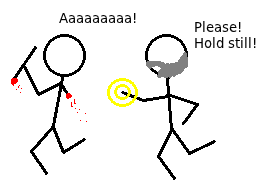
\includegraphics{Pics/Regenerate.png}
\end{figure*}

The subject's severed body members (fingers, toes, hands, feet, arms, legs, tails, or even heads of multiheaded creatures), broken bones, and ruined organs grow back. 
After the spell is cast, the physical regeneration is complete in 1 round if the severed members are present and touching the creature. It takes 2d10 rounds otherwise.
This regeneration is instantaneous in nature.

Regenerate also grants the subject Fast Healing 3 for 1 minute, rids the subject of \emph{exhaustion} and/or \emph{fatigue}, and eliminates all nonlethal damage the subject has taken.
It has no effect on nonliving creatures (including undead).

\paragraph{Augment:} If you spend 2 additional spell points and 200XP, you can target this spell on the remains of a creature that has been dead for no longer than 1 round.
The creature then immediately comes back to life, at -9 hit points. It suffers no level loss, loss of constitution, or other usual drawbacks of dying, since this spell acts before the subject's soul has fully left the body.
If the creature's remains were in a especially bad state (such as due to death by decapitation, or a \nameref{Spell:Disintegrate} or \nameref{Spell:Implosion} spell), it takes 2d10 rounds for the creature to reform its body, during which time it cannot act.
Even if the subject's remains were mostly intact and its hit points are brought into the positives, it cannot act for one round after being brought back to life in this way, since the spell needs time to repair the lethal damage.
The spell's other functions affect the creature normally. It gains Fast Healing 3 for 1 minute, and is cured of all \emph{exhaustion}, \emph{fatigue}, and nonlethal damage.
\subsubsection{Reincarnate}
\label{Spell:Reincarnate}
Necromancy (Healing)
\\ \textbf{Level:} Chaos 4
\\ \textbf{Components:} V, S
\\ \textbf{Casting Time:} 1 minute
\\ \textbf{Range:} Touch
\\ \textbf{Target:} Dead creature touched
\\ \textbf{Duration:} Instantaneous
\\ \textbf{Saving Throw:} None; see text
\\ \textbf{Spell Resistance:} Yes (harmless)
\\ \textbf{Spell Points:} 7; XP; see text

\emph{''This body is finished. But I can create a new one.``}

You restore life to a deceased creature by creating a new body for it. 
You can raise a creature that has been dead for no longer than one week. 
In addition, the subject's soul must be free and willing to return. 
If the subject's soul is not willing to return, the spell does not work; 
therefore, a subject that wants to return receives no saving throw.

Since the dead creature is returning in a new body, all physical ills and afflictions are repaired 
(including ability damage, ability drain, as well as normal disease and poison, but not curses or magical diseases).
The condition of the remains is not a factor.
So long as some small portion of the creature's body still exists, 
it can be reincarnated, but the portion receiving the spell must have been part of the creature's body at the time of death. 
The magic of the spell creates an entirely new body (of an age category equal to that of the subject's previous body) 
for the soul to inhabit from the natural elements at hand.
The new body may be of a race different from the creature's original.
This process takes 1 hour to complete. When the body is ready, the subject is reincarnated.
A reincarnated creature has a number of hit points equal to its current Hit Dice.
None of the dead creature's equipment or possessions are affected in any way by this spell.

Coming back from the dead is an ordeal. 
The subject of the spell loses one level (or 1 Hit Die) when it is raised, 
just as if it had lost a level or a Hit Die to an energy-draining creature. 
If the subject is 1st level, 
it loses 2 points of Constitution instead (if this would reduce its Con to 0 or less, it can't be raised). 
This level/HD loss or Constitution loss cannot be repaired by any means (if the character's race changes, determine its ability score changes first). 
A character who died with unused spell points comes back with 50\% of them (rounded down, minimum 0).
The potential spell point loss for losing a level won't come in until the next time the raised character replenishes his spell points.

A creature who has been turned into an undead creature or killed by a death effect can't be raised by this spell. 
Constructs, elementals, outsiders, and undead creatures can't be raised. 
The spell cannot bring back a creature that has died of old age.

To determine the race of the creature's new body, roll on the \nameref{tab:Reincarnate} table.

Whatever the result, a Reincarnate spell can never result in a creature's level adjustment or number of hit dice
(aside from level loss, see above) changing.\\
\begin{tableonecolumn}
\caption{Reincarnate}
\label{tab:Reincarnate}
\begin{tabular}{ll}
\toprule
d\%	&Incarnation\\
\midrule
$\leq$5	&Caster's race\\
6-10	&Target's choice (other than old race)\\
11-40	&Same as old race\\
41-50	&Related race (GM's adjucation)\\
51-60	&Decidedly unrelated race (GM's adjucation)\\
61-90	&Roll randomly among races in the setting\\
91+	&GM's choice\\
\bottomrule
\end{tabular}
\end{tableonecolumn}

To determine the ability scores of a reincarnated creature, eliminate its old racial adjustments to ability scores,
and add the racial adjustments of its new race (including mental ability scores).
The reincarnated creature gains all abilities associated with its new form, 
including forms of movement and speeds, natural armor, natural attacks, extraordinary abilities, and the like, 
but it doesn't automatically speak the language of the new form. 

If the subject's race changes, it hereafter ages as a creature of its new race.
For example, an orc that reached middle age just before being reincarnated as an elf ages from that point as any other elf
that just reached middle age (even if the character's absolute age would not even place it as an adult for naturally born elves).
For venerable creatures, reroll the maximum age according to its new race.

\paragraph{Augment:} This spell can be augmented in one or more of the following ways:
\begin{enumerate}
 \item If you spend 2 additional spell points and 500 additional XP, 
the creature can have been dead no longer than 10 years per caster level rather than one week.
 \item If you spend an additional spell point and 250 additional XP, a spellcaster being raised does not
lose any spell points as part of returning from the dead.
 \item If you spend an additional spell point and 250 additional XP, 
curses and magical diseases are cured as part of the subject returning from the dead.
 \item If you spend 2 additional spell points and 250 additional XP, 
you can reincarnate someone killed by a death effect.
 \item If you spend 8 additional spell points and 4000 additional XP,
the subject of the spell does not lose a level or points of constitution (other than due to a change in the subject's race) when it is reincarnated.
\end{enumerate}

\emph{Experience Cost:} 200XP.
\subsubsection{Remove Blindness or Deafness}
\label{Spell:RemoveBlindnessDeafness}
Necromancy (Healing)
\\ \textbf{Level:} Paladin 3
\\ \textbf{Components:} V, S
\\ \textbf{Casting Time:} 1 standard action
\\ \textbf{Range:} Touch
\\ \textbf{Target:} Creature touched
\\ \textbf{Duration:} Instantaneous
\\ \textbf{Saving Throw:} Fortitude negates (harmless)
\\ \textbf{Spell Resistance:} Yes (harmless)
\\ \textbf{Spell Points:} 5

\emph{''No, my good man, it's really not a Miracle. Just the cure for blindness.``}

This spell cures blindness, deafness, or damage to or loss of any one special sense (such as scent, blindsight, blindsense, or tremorsense). 
Whether the effect is normal or magical in nature does not matter.
The spell does not restore ears or eyes that have been lost, but it repairs them if they are damaged.

\paragraph{Augment:} For every 2 additional spell points you spend, this spell can affect an additional creature.

\subsubsection{Remove Curse}
\label{Spell:RemoveCurse}
Abjuration
\\ \textbf{Level:} Bard 3, Healing 3, Luck 3, Paladin 3, Sor/Wiz 4
\\ \textbf{Components:} V, S
\\ \textbf{Casting Time:} 1 minute
\\ \textbf{Range:} Touch
\\ \textbf{Target:} Creature or item touched
\\ \textbf{Duration:} Instantaneous
\\ \textbf{Saving Throw:} Will negates (harmless)
\\ \textbf{Spell Resistance:} Yes (harmless)
\\ \textbf{Spell Points:} Bard 5, Healing 5, Luck 5, Paladin 5, Sor/Wiz 7

\emph{Many magical maladies exist, and this is the cure for most of them.}

Remove curse instantaneously removes all curses on an object or a creature. 
Remove curse does not remove the curse from a cursed shield, weapon, or suit of armor, although the spell typically enables the creature afflicted with any such cursed item to remove and get rid of it. 
Certain special curses may not be countered by this spell or may be countered only by a caster of a certain level or higher.

\paragraph{Augment:} This spell can be augmented in one or both of the following ways:
\begin{enumerate}
 \item For every 2 additional spell points you spend, this spell can affect an additional creature.
 \item If you spend 2 additional spell points, the spell can free victims from certain powerful spells (particularly enchantments and transmutations) in addition to curses.
The spell can then reverse even an instantaneous effect. An effect that requires this augment will specify that it does.

For each such effect, you make a caster level check (1d20 + caster level) against a DC of 11 + caster level of the effect.
Success means that the creature is free of the spell, curse, or effect. For a cursed magic item, the DC is 25.
\end{enumerate}

\paragraph{Special:} If the spell to be removed is one that cannot be dispelled by \nameref{Spell:DispelMagic}, this spell works only if that spell was cast using fewer spell points than were spent on casting this spell.
\subsubsection{Remove Disease}
\label{Spell:RemoveDisease}
Necromancy (Healing)
\\ \textbf{Level:} Healing 3, Paladin 3, Ranger 3
\\ \textbf{Components:} V, S
\\ \textbf{Casting Time:} 1 standard action
\\ \textbf{Range:} Touch
\\ \textbf{Target:} Creature touched
\\ \textbf{Duration:} Instantaneous
\\ \textbf{Saving Throw:} Fortitude negates (harmless)
\\ \textbf{Spell Resistance:} Yes (harmless)
\\ \textbf{Spell Points:} 5

\emph{''Plague? No problem.``}

Remove disease cures all diseases that the subject is suffering from. 
The spell also kills parasites, including green slime and others. 
Certain special diseases may not be countered by this spell or may be countered only by a caster of a certain level or higher.

\emph{Note:} Since the spell's duration is instantaneous, it does not prevent reinfection after a new exposure to the same disease at a later date.

\paragraph{Augment:} For every 2 additional spell points you spend, this spell can affect an additional creature.
\subsubsection{Remove Fear}
\label{Spell:RemoveFear}
Abjuration
\\ \textbf{Level:} Bard 1, Healing 1, Paladin 1
\\ \textbf{Components:} V, S
\\ \textbf{Casting Time:} 1 standard action
\\ \textbf{Range:} Touch
\\ \textbf{Targets:} One creature
\\ \textbf{Duration:} 1 round/level
\\ \textbf{Saving Throw:} Will negates (harmless)
\\ \textbf{Spell Resistance:} Yes (harmless)
\\ \textbf{Spell Points:} 1

\emph{Your fear does not go anywhere. But it no longer impedes you.}

The subject gains immunity to fear effects.

\paragraph{Augment:} You can augment this spell in one or both of the following ways:
\begin{enumerate}
 \item For every 2 additional spell points you spend, this spell can affect an additional creature.
 \item If you spend 2 additional spell points, the spell's duration increases to 10 minutes per level.
\end{enumerate}
\subsubsection{Remove Paralysis}
\label{Spell:RemoveParalysis}
Conjuration (Healing)
\\ \textbf{Level:} Healing 2
\\ \textbf{Components:} V, S
\\ \textbf{Casting Time:} 1 standard action
\\ \textbf{Range:} Close (25 ft. + 5 ft./2 levels)
\\ \textbf{Target:} One creature
\\ \textbf{Duration:} Instantaneous
\\ \textbf{Saving Throw:} Will negates (harmless)
\\ \textbf{Spell Resistance:} Yes (harmless)
\\ \textbf{Spell Points:} 3

\emph{''Stand up! It's just paralysis!``}

You can free one creature from the effects of any temporary \emph{paralysis} or related magic, including a ghoul's touch or a \nameref{Spell:Slow} spell. It does not heal creatures who have been permanently paralyzed in mundane circumstances (such creatures who have taken spinal damage).

The spell does not restore ability scores reduced by penalties, damage, or drain.

\paragraph{Augment:} You can augment this spell in one or both of the following ways:
\begin{enumerate}
 \item For every two additional spell points you spend, this spell can affect an additional creature. No two recipients of the spell may be more than 30' apart. 
 \item If you spend 10 additional spell points, you can heal mundane paralysis.
\end{enumerate}
\subsubsection{Repair}
\label{Spell:Repair}
Transmutation
\\ \textbf{Level:} Bard 1, Sor/Wiz 1
\\ \textbf{Components:} V, S
\\ \textbf{Casting Time:} 1 standard action
\\ \textbf{Range:} Touch
\\ \textbf{Target:} One object of up to 1 lb./level OR construct touched; See text
\\ \textbf{Duration:} Instantaneous
\\ \textbf{Saving Throw:} Will negates (harmless)
\\ \textbf{Spell Resistance:} Yes (harmless)
\\ \textbf{Spell Points:} 1, XP; see text

\emph{''Reparo!``}

The spell has two separate functions, \emph{Mending} (which affects items) and \emph{Repair construct} (which affects constructs). 
Each has its own usage descriptions and augmentation options.
\begin{itemize}
 \item \emph{Mending:} This function of the spell repairs breaks or tears in objects, making it strong as new. 
It will completely repair broken objects up to its weight limit, regardless of the number of breaks, so long as all the pieces are present.
The spell can repair a magic item, but the item's magical abilities are not restored. 
The spell cannot mend broken magic rods, staffs, or wands,

\paragraph{Augment:} You can Augment the Mending function of the spell in one of the following ways:
\begin{enumerate}
 \item If you spend two additional spell points, the weight limit of the spell increases to 10 lb./level.
 \item If you spend six additional spell points, the weight limit of the spell increases to 100 lb./level.
 \item If you spend eight additional spell points, the spell restores the magical abilities of a broken magic item when it repairs such an item.
 It can mend broken magic rods, staffs and wands, restoring their status to what it was at the time the item was broken. It never restores spent charges.
 \item If you spend sixteen additional spell points, the spell can restore the magical properties of a magic item (other than an artifact) that
 has been drained of magic by a \nameref{Spell:Disjunction} spell. 
 This use of the spell requires you to expend a number of experience points equal to the number required to craft the item in the first place.
\end{enumerate}
\item \emph{Repair Construct:} When laying your hands upon a construct that has at least 1 hit point remaining, 
you reknit its structure to repair damage it has taken. 
The spell repairs 1d8 points of damage +1 point per caster level. 
Constructs that are immune to magic cannot be repaired in this fashion.

\paragraph{Augment:} For every 2 additional spell points you spend, the Repair construct function of the spell repairs an additional 1d8 points of damage.
\end{itemize}
\subsubsection{Repel Metal and Stone}
\label{Spell:RepelMetalAndStone}
Abjuration [Earth]
\\ \textbf{Level:} Earth 8
\\ \textbf{Components:} V, S
\\ \textbf{Casting Time:} 1 standard action
\\ \textbf{Range:} 60 ft.
\\ \textbf{Area:} 60-ft. line from you
\\ \textbf{Duration:} 1 round/level (D)
\\ \textbf{Saving Throw:} None
\\ \textbf{Spell Resistance:} No
\\ \textbf{Spell Points:} 15

\emph{Waves of invisible and intangible energy roll forth from you.}

All metal or stone objects in the path of the spell are pushed away from you to the limit of the range. 
Fixed metal or stone objects larger than 3 inches in diameter and loose objects weighing more than 500 pounds are not affected. 
Anything else, including animated objects, small boulders, and creatures in metal armor, moves back. 
Fixed objects 3 inches in diameter or smaller bend or break, and the pieces move with the wave of energy. 
Objects affected by the spell are repelled at the rate of 40 feet per round.

Objects such as metal armor, swords, and the like are pushed back, dragging their bearers with them. A creature being dragged by an item it is carrying can let go. A creature being dragged by a shield can loose it as a move action and drop it as a free action.
Even magic items with metal components are repelled.

After you cast the spell, its area and direction path are set, and you can then do other things or go elsewhere without affecting the spell's power.

\paragraph{Augment:} If you spend 2 additional spell points, this spell's range changes to 10', and its area changes to a 10' radius emanation, centered on you.
The spell then follows you around, remaining centered on you for the duration.
\subsubsection{Repel Vermin}
\label{Spell:RepelVermin}
Abjuration
\\ \textbf{Level:} Bard 4, Ranger 4, Vermin 4
\\ \textbf{Components:} V, S
\\ \textbf{Casting Time:} 1 standard action
\\ \textbf{Range:} 10 ft.
\\ \textbf{Area:} 10-ft.-radius emanation centered on you
\\ \textbf{Duration:} 10 min./level (D)
\\ \textbf{Saving Throw:} None or Will negates; see text
\\ \textbf{Spell Resistance:} Yes
\\ \textbf{Spell Points:} 7

\emph{You create an invisible barrier to hold back vermin.} 

A vermin with 3 Hit Dice or less cannot enter within the radius of the emanation. 
This includes all swarms consisting of vermin, regardless of the swarm's total number of Hit Dice.

A vermin with more than 3 Hit Dice can penetrate the barrier if it succeeds on a Will save. 
Even so, crossing the barrier deals the vermin 2d6 points of damage, and pressing against the barrier causes pain, which deters most vermin.

\paragraph{Augment:} For every 2 additional spell points you spend, the emanation prevents the entry of creatures with one additional Hit Die, and the damage dealt to higher HD vermin who manage to cross is increased by one die (d6).
\subsubsection{Repel Wood}
\label{Spell:RepelWood}
Abjuration [Earth]
\\ \textbf{Level:} Plant 6, Ranger 6
\\ \textbf{Spell Points:} 11

\emph{Waves of warm energy softly emanate out from your position.}

This spell functions as \nameref{Spell:RepelMetalAndStone} (including its augmentation option), except as noted here, and it affects objects made of wood (such as wooden shields, spears, wooden weapon shafts and hafts, and arrows and bolts), rather than objects of metal and stone.

\subsubsection{Resilient Sphere}
\label{Spell:ResilientSphere}
Evocation [Force]
\\ \textbf{Level:} Evoker 4
\\ \textbf{Components:} V, S
\\ \textbf{Casting Time:} 1 standard action
\\ \textbf{Range:} Close (25 ft. + 5 ft./2 levels)
\\ \textbf{Effect:} Sphere of force, centered around a medium-sized or smaller creature
\\ \textbf{Duration:} 1 min./level (D)
\\ \textbf{Saving Throw:} Reflex negates
\\ \textbf{Spell Resistance:} Yes
\\ \textbf{Spell Points:} 7

\emph{''You're not going anywhere.``}

A globe of shimmering, transparent force encloses a creature of size medium or smaller. 
The sphere contains its subject for the spell's duration. 
The sphere is not subject to damage of any sort except from a rod of cancellation, 
a rod of negation, a \nameref{Spell:Disintegrate} spell, or a targeted \nameref{Spell:DispelMagic} spell. 
These effects destroy the sphere without harm to the subject. 
Nothing can pass through the sphere, inside or out, though the subject can breathe normally.

The subject may struggle, but the sphere cannot be physically moved either by people outside it or by the struggles of those within.

\paragraph{Augment:} You can augment this spell in one or more of the following ways.

\begin{enumerate}
 \item If you spend 6 additional spell points, this spell does not offer a saving throw.
 \item For every 3 additional spell points you spend, this spell can affect a creature one size category larger than medium.
 \item If you spend 6 additional spell points, 
you can telekinetically move the sphere as long as its contents weigh 5,000 pounds or less. 
The telekinetic control extends from you out to medium range (100 feet + 10 feet per caster level) after the sphere has succeeded in encapsulating its contents.
You can move objects or creatures in the sphere that weigh a total of 5,000 pounds or less by concentrating on the sphere. 
You can begin moving a sphere in the round after casting the spell. 
If you concentrate on doing so (a standard action), you can move the sphere as much as 30 feet in a round. 
If you cease concentrating, the sphere does not move in that round (if on a level surface) or descends at its falling rate (if aloft) until it reaches a level surface, 
or the spell's duration expires, or you begin concentrating again. 
If you cease concentrating (voluntarily or due to failing a Concentration check), you can resume concentrating on your next turn or any later turn during the spell's duration.

The sphere falls at a rate of only 60 feet per round, which is not fast enough to cause damage to the contents of the sphere.

You can move the sphere telekinetically even if you are in it. 
\end{enumerate}
\subsubsection{Resistance}
\label{Spell:Resistance}
Abjuration
\\ \textbf{Level:} Abjurer 2, Blackguard 2, Paladin 2, Protection 2, Ranger 2
\\ \textbf{Components:} V, S
\\ \textbf{Casting Time:} 1 standard action
\\ \textbf{Range:} Touch
\\ \textbf{Target:} Creature touched
\\ \textbf{Duration:} 10 min./level
\\ \textbf{Saving Throw:} Will negates (harmless)
\\ \textbf{Spell Resistance:} Yes (harmless)
\\ \textbf{Spell Points:} 3

\emph{You defend the subject with the most general of abjurations.}

This spell grants a +1 resistance bonus on saving throws.

\paragraph{Augment:} You can augment this spell in one or both of the following ways.
\begin{enumerate}
\item For every three additional spell points you spend, the resistance bonus increases by 1.
\item If you spend two additional spell points, the spell's duration increases to 24 hours.
\end{enumerate}

\subsubsection{Resist Energy}
\label{Spell:ResistEnergy}
Abjuration
\\ \textbf{Level:} Blackguard 2, Fire 2, Paladin 2, Ranger 2, Sor/Wiz 2
\\ \textbf{Components:} V, S
\\ \textbf{Casting Time:} 1 standard action
\\ \textbf{Range:} Touch
\\ \textbf{Target:} Creature touched
\\ \textbf{Duration:} 10 min./level
\\ \textbf{Saving Throw:} Will negates (harmless)
\\ \textbf{Spell Resistance:} Yes (harmless)
\\ \textbf{Spell Points:} 3

\emph{Suddenly, the elements no longer seem all that frightening.}

The subject of this spell gains resistance 10 against acid, cold, electricity, fire or sonic damage, chosen at the time of casting.

The energy resistance provided by this spell increases to 20 points at caster level 9th, and to its maximum of 30 at 13th level.
The spell protects equipment as well.

\paragraph{Augment:} You can augment this spell in one or both of the following ways.
\begin{enumerate}
\item If you spend four additional spell points, the subject gains resistance to all the listed energy types, rather than just one.
\item If you spend four additional spell points, you can cast this spell as an immediate action.
\end{enumerate}
\subsubsection{Restoration}
\label{Spell:Restoration}
Necromancy (Healing)
\\ \textbf{Level:} Healing 2, Paladin 2
\\ \textbf{Components:} V, S
\\ \textbf{Casting Time:} 3 rounds
\\ \textbf{Range:} Touch
\\ \textbf{Target:} Creature touched
\\ \textbf{Duration:} Instantaneous
\\ \textbf{Saving Throw:} Will negates (harmless)
\\ \textbf{Spell Resistance:} Yes (harmless)
\\ \textbf{Spell Points:} 3

\emph{The creature breathes more easily.}

Restoration dispels any magical effects reducing one of the subject's ability scores or cures 1d4 points of temporary ability damage to one of the subject's ability scores. 
It also eliminates any fatigue suffered by the character, and improves an exhausted condition to fatigued. 
It does not restore permanent ability drain.

\paragraph{Augment:} You can augment this spell in one or more of the following ways:
\begin{enumerate}
 \item If you spend 4 additional spell points, this spell also dispels negative levels and restores one experience level to a creature who has had a level drained. The drained level is restored only if the time since the creature lost the level is equal to or less than one day per caster level. 
A character who has a level restored by restoration has exactly the minimum number of experience points necessary to restore him or her to his or her previous level.
This augment does not restore levels or Constitution points lost due to death.
 \item If you spend 4 additional spell points, this spell cures all temporary ability damage, and it restores all points permanently drained from a single ability score (your choice if more than one is drained). 
It also eliminates any fatigue or exhaustion suffered by the target.
 \item If you spend 10 additional spell points and 500XP, this spell removes all forms of insanity, confusion, and similar mental effects.
\end{enumerate}
\subsubsection{Reverse Gravity}
\label{Spell:ReverseGravity}
Abjuration
\\ \textbf{Level:} Sor/Wiz 7, Travel 7
\\ \textbf{Components:} V, S
\\ \textbf{Casting Time:} 1 standard action
\\ \textbf{Range:} Medium (100 ft. + 10 ft./level)
\\ \textbf{Target:} One creature
\\ \textbf{Duration:} Instantaneous
\\ \textbf{Saving Throw:} None
\\ \textbf{Spell Resistance:} Yes
\\ \textbf{Spell Points:} 13

\emph{''Enjoy your flight.``}

You change the way gravity affects the target creature.
The creature instantaneously ''falls'' 500' in any direction (other than down).
This fall is treated as an ordinary fall in all respects - the target takes the appropriate falling damage if it hits something on the way (such as the ceiling),
the \nameref{Spell:ControlFall} spell makes it fall 60' rather than 500', a creature with a Fly speed is not affected unless it wishes to, 
and the target (or those near to it) may use the Climb skill to catch itself as it falls.

Reality rapidly compensates for this breach of the laws of physics, making traditional ballistics inapplicable.\footnote{\emph{Optional rule:}
Ballistics apply. Rather than ``falling 500''', the effects of gravity on the subject are ignored for one round, and a force with an equal magnitude
but different direction is applied to the subject for the same duration. 
This approach is recommended only if someone at the table has a talent for on-the-fly vector calculus.}
If you cause the creature to fall at an angle, 
refer to the \nameref{tab:ReverseGravity} table for a reference on the vertical and horizontal distances the subject falls.
\begin{tableonecolumn}
\caption{Reverse Gravity Angle Examples}
\label{tab:ReverseGravity}
\begin{tabular}{rrr}
\toprule
Angle$^1$	&Horizontal	&Maximum\\
		&distance$^2$	&height$^2$\\
\midrule
 0$^\circ$	&500 feet	&  0 feet\\
15$^\circ$	&485 feet	&130 feet\\
30$^\circ$	&435 feet	&250 feet\\
45$^\circ$	&355 feet	&355 feet\\
60$^\circ$	&250 feet	&435 feet\\
75$^\circ$	&130 feet	&485 feet\\
90$^\circ$	&  0 feet	&500 feet\\
\bottomrule
\end{tabular}
\begin{enumerate}
 \item An angle with respect to the ground the creature was standing on.
 \item With respect to the ground the creature was standing on.
\end{enumerate}

\end{tableonecolumn}
A creature always falls straight down after travelling 500' in this fashion.

\paragraph{Augment:} For every 2 additional spell points you spend, this spell affects an additional creature within range.
\subsubsection{Righteous Might}
\label{Spell:RighteousMight}
Transmutation [see text]
\\ \textbf{Level:} Blackguard 5, Paladin 5, Strength 5, War 5
\\ \textbf{Components:} V, S
\\ \textbf{Casting Time:} 1 standard action
\\ \textbf{Range:} Personal
\\ \textbf{Target:} You
\\ \textbf{Duration:} 1 round/level (D)
\\ \textbf{Spell Points:} 9

\emph{``By the power of Greyskull!''}

\begin{figure*}
  \caption{Cleric uses Righteous Might to match the combat prowess of a superior foe.}
  \centering
    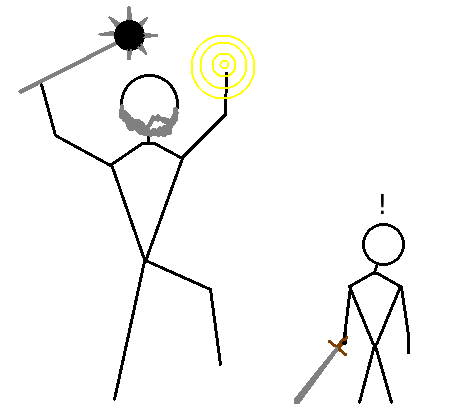
\includegraphics{Pics/RighteousMight.png}
\end{figure*}

Your height is doubled, your weight is multiplied by 8, and your size category increases to the next larger one.
You gain a +4 size bonus to Strength, a +2 size bonus to Constitution, 
and your size modifier for AC and attacks changes as appropriate to your new size category.
You gain a +2 enhancement bonus to your natural armor.
At the time you cast this spell, choose an alignment you wish to protect yourself against.
You gain DR 3/that alignment. The spell gains a descriptor opposed to that alignment
(for example, if you choose to gain DR/evil, this becomes a Transmutation [Good] spell).

A humanoid creature whose size increases to Large has a space of 10 feet and a natural reach of 10 feet.
If insufficient room is available for the desired growth, 
you attain the maximum possible size and may make a Strength check 
(using your increased Strength) to burst any enclosures in the process. 
If the check fails, you are constrained without harm by the materials enclosing you - 
you cannot crush yourself by increasing your size.

This spell does not change your speeds.

All equipment worn or carried by you has its size similarly altered by the spell. 
See Table: Larger and Smaller Weapon Damage for effects on the damage of weapons.
Note the effects of your changed carrying capacity.
Any item that leaves your possession while you have had your size altered (including a projectile or thrown weapon) 
instantly returns to its normal size. 
This means that thrown weapons deal their normal damage, and projectiles deal damage based on the size of the weapon that fired them. 

\paragraph{Augment:} If you spend 6 additional spell points, 
your height is tripled, your weight is multiplied sixteenfold, 
and your size category increases by two instead of one.
You instead gain a +6 size bonus to Strength, and a +3 enhanchement bonus to your natural armor.

In addition, for every additional spell point you spend, 
the damage reduction offered by this spell increases by 1.

\subsubsection{Rusting Grasp}
\label{Spell:RustingGrasp}
Transmutation
\\ \textbf{Level:} Destruction 4, Water 4
\\ \textbf{Components:} V, S
\\ \textbf{Casting Time:} 1 standard action
\\ \textbf{Range:} Touch
\\ \textbf{Target:} One nonmagical ferrous object (or the volume of the object within 3 ft. of the touched point) or one ferrous creature
\\ \textbf{Duration:} See text
\\ \textbf{Saving Throw:} None
\\ \textbf{Spell Resistance:} No
\\ \textbf{Spell Points:} 7

\emph{``An Iron Golem, you say? I have just the thing.''}

Any iron or iron alloy item you touch becomes instantaneously rusted, pitted, and useless. If the item is so large that it cannot fit within a 3-foot radius a 3-foot-radius volume of the metal is rusted and destroyed. Magic items made of metal are immune to this spell.
Provided all the rusted remains are present, a \nameref{Spell:Repair} spell can restore an item to its former status.

You may employ rusting grasp in combat with a successful melee touch attack. Rusting grasp used in this way instantaneously destroys 1d6 points of Armor Class gained from metal armor (to the maximum amount of protection the armor offered) through corrosion.

Weapons in use by an opponent targeted by the spell are more difficult to grasp. You must succeed on a melee touch attack against the weapon. A metal weapon that is hit is destroyed.
Striking at an opponent's weapon in this way provokes an attack of opportunity unless you have the Improved Sunder feat. Also, you must touch the weapon and not the other way around.

Against a ferrous creature, rusting grasp instantaneously deals 7d6 points of damage per successful attack. 

The spell lasts for 1 round per level, and you can make one melee touch attack per round.

\paragraph{Augment:} If you spend 2 additional spell points, magic items made of metal are not immune to this spell.
\subsection{'S' Spells}
\subsubsection{Sanctuary}
\label{Spell:Sanctuary}
Abjuration
\\ \textbf{Level:} Protection 1
\\ \textbf{Components:} V, S,
\\ \textbf{Casting Time:} 1 standard action
\\ \textbf{Range:} Touch
\\ \textbf{Target:} Creature touched
\\ \textbf{Duration:} 1 round/level
\\ \textbf{Saving Throw:} Will negates
\\ \textbf{Spell Resistance:} No
\\ \textbf{Spell Points:} 1

\emph{You take the fundamental injustice involved when a violent man attacks an innocent, and turn it into a shield.}

Any opponent attempting to strike or otherwise directly attack the warded creature, even with a targeted spell, must attempt a Will save. 
If the save succeeds, the opponent can attack normally and is unaffected by that casting of the spell. 
If the save fails, the opponent can't follow through with the attack, that part of its action is lost, and it can't directly attack the warded creature for the duration of the spell. 
Those not attempting to attack the subject remain unaffected. 
This spell does not prevent the warded creature from being attacked or affected by area or effect spells. 
The subject cannot attack without breaking the spell but may use nonattack spells or otherwise act.

\paragraph{Augment:} If you spend 10 additional spell points, this spell's duration increases to 24 hours.
\subsubsection{Scorching Ray}
\label{Spell:ScorchingRay}
Evocation [see text]
\\ \textbf{Level:} Sor/Wiz 1
\\ \textbf{Components:} V, S
\\ \textbf{Casting Time:} 1 standard action
\\ \textbf{Range:} Close (25 ft. + 5 ft./2 levels)
\\ \textbf{Effect:} Ray
\\ \textbf{Duration:} Instantaneous
\\ \textbf{Saving Throw:} None
\\ \textbf{Spell Resistance:} Yes
\\ \textbf{Spell Points:} 1

\emph{This simplest of evocations remains as one as the most reliable.}

At the time of casting, you choose between cold, electricity, fire, or sonic damage. 

You create a ray of energy of the chosen type that shoots forth from your fingertip and strikes a target within range, 
dealing 1d6 points of damage, if you succeed on a ranged touch attack with the ray.

\begin{itemize}
 \item Cold: A ray of this energy type deals +1 point of damage per die.
 \item Electricity: Casting a ray of this energy type provides a +3 bonus on your attack roll if the target is wearing metal armor 
 and a +2 bonus on caster level checks for the purpose of overcoming spell resistance.
 \item Fire: A ray of this energy type deals +1 point of damage per die. (This was the form of the spell that was discovered first among Evokers.
 Although further research showed that the same spell could produce the other energy types with minimal modifications, the name of ''scorching ray`` stuck.)
 \item Sonic: A ray of this energy type deals -1 point of damage per die and ignores an object's hardness.
\end{itemize}

This spell's descriptor is the same as the type of energy you selected. 

\paragraph{Augment:} For every additional spell point you spend, this spell's damage increases by one die (d6).
\subsubsection{Screen}
\label{Spell:Screen}
Illusion (Glamer)
\\ \textbf{Level:} Illusionist 8, Trickery 7
\\ \textbf{Components:} V, S
\\ \textbf{Casting Time:} 10 minutes
\\ \textbf{Range:} Close (25 ft. + 5 ft./2 levels)
\\ \textbf{Area:} 30-ft. cube/level (S)
\\ \textbf{Duration:} 24 hours
\\ \textbf{Saving Throw:} None or Will disbelief (if interacted with); see text
\\ \textbf{Spell Resistance:} No
\\ \textbf{Spell Points:} Illusionist 15, Trickery 13

\emph{This spell combines several elements to create a powerful protection from scrying and direct observation. }

When casting the spell, you dictate what will and will not be observed in the spell's area. 
The illusion created must be stated in general terms. Once the conditions are set, they cannot be changed.

Attempts to scry the area automatically detect (do not penetrate) the image stated by you with no save allowed. 
Sight and sound are appropriate to the illusion created.

Direct observation may allow a save (as per a normal illusion), 
if there is cause to disbelieve what is seen. 
Even entering the area does not cancel the illusion or necessarily allow a save, 
assuming that hidden beings take care to stay out of the way of those affected by the illusion. 
\subsubsection{Scrying}
\label{Spell:Scrying}
Divination (Scrying)
\\ \textbf{Level:} Bard 3, Diviner 4, Knowledge 4
\\ \textbf{Components:} V, S
\\ \textbf{Casting Time:} 1 hour
\\ \textbf{Range:} See text
\\ \textbf{Effect:} Magical sensor next to a creature
\\ \textbf{Duration:} 1 min./level
\\ \textbf{Saving Throw:} Will negates
\\ \textbf{Spell Resistance:} Yes
\\ \textbf{Spell Points:} Bard 5, Diviner 7, Knowledge 7

\emph{Distances suddenly mean very little to your ability to glean information.}

You can see and hear some creature, which may be at any distance. 
If the subject succeeds on a Will save, the scrying attempt simply fails. 
The difficulty of the save depends on how well you know the subject and what sort of physical connection (if any) you have to that creature (see the \nameref{tab:Scrying} table). 

If the save fails, you can see and hear the subject and the subject's immediate surroundings (approximately 10 feet in all directions of the subject). 
If the subject moves, the scrying sensor follows, regardless of its speed.
If it uses a teleportation spell to move more than 10 feet or crosses planar boundaries, however, the spell ends.

The sensor has your full visual acuity, including any magical effects. %In addition, 
%the following spells have a 5\% chance per caster level of operating through the sensor: 
%detect chaos, detect evil, detect good, detect law, detect magic, and message.

If the save succeeds, you can't attempt to scry on that subject again for 24 hours.

\begin{table*}
\caption{Scrying save modifiers}
\label{tab:Scrying}
\begin{center}
\begin{tabular}{lc}
\toprule
Knowledge & Will Save Modifier$^1$\\
\midrule
None$^2$&+10\\
Secondhand (you have heard of the subject)&+5\\
Firsthand (you have met the subject)&+0\\
Familiar (you know the subject well)&-5\\
\midrule
Connection&Will Save Modifier\\
\midrule
Likeness or picture&-2\\
Possession or garment&-4\\
Body part, lock of hair, bit of nail, etc.&-10\\
Subject is on another plane&+5\\
\bottomrule
\end{tabular}
\begin{enumerate}
 \item Modifiers are cumulative.
 \item You must have some sort of connection to a creature you have no knowledge of.
\end{enumerate}
\end{center}
\end{table*}

\paragraph{Augment:} If you spend 6 additional spell points, you can cast this spell as a standard action.

\subsubsection{Sculpt Sound}
\label{Spell:SculptSound}
Transmutation
\\ \textbf{Level:} Bard 3
\\ \textbf{Components:} V, S
\\ \textbf{Casting Time:} 1 standard action
\\ \textbf{Range:} Close (25 ft. + 5 ft./2 levels)
\\ \textbf{Targets:} Five creatures or objects, no two of which can be more than 30 ft. apart
\\ \textbf{Duration:} 1 hour/level (D)
\\ \textbf{Saving Throw:} Will negates (object)
\\ \textbf{Spell Resistance:} Yes (object)
\\ \textbf{Spell Points:} 5

\emph{''Those very very serious guards would be much funnier with squeaky shoes, don't you agree?``}

You change the sounds that creatures or objects make. You can create sounds where none exist, deaden or completely silence sounds, or transform sounds into other sounds. All affected creatures or objects must be transmuted in the same way. Once the transmutation is made, you cannot change it.

You can change the qualities of sounds but cannot create words with which you are unfamiliar yourself.

A spellcaster whose voice is silenced or changed dramatically is unable to cast spells with verbal components.

\paragraph{Augment:} For every additional spell point you spend, this spell can affect an additional creature.

\subsubsection{Searing Light}
\label{Spell:SearingLight}
Evocation
\\ \textbf{Level:} Sun 1
\\ \textbf{Components:} V, S
\\ \textbf{Casting Time:} 1 standard action
\\ \textbf{Range:} Medium (100 ft. + 10 ft./level)
\\ \textbf{Effect:} Ray
\\ \textbf{Duration:} Instantaneous
\\ \textbf{Saving Throw:} None
\\ \textbf{Spell Resistance:} Yes
\\ \textbf{Spell Points:} 1

\emph{Focusing divine power like a ray of the sun, you project a blast of light from your open palm. }

You must succeed on a ranged touch attack to strike your target.
Undead creatures and oozes struck by the ray take 1d6 points of damage, objects and other creatures take half damage.
A creature that is harmed by or takes penalties from sunlight or bright light takes double damage (meaning that a non-undead, non-ooze creature that takes penalties from light takes normal damage).

\paragraph{Augment:} For every additional spell point you spend, the damage against undead creatures and oozes increases by 1d6 (with a corresponding increase in damage against other creatures).

\subsubsection{See Invisibility}
\label{Spell:SeeInvisibility}
Divination
\\ \textbf{Level:} Bard 2, Sor/Wiz 2
\\ \textbf{Components:} V, S
\\ \textbf{Casting Time:} 1 standard action
\\ \textbf{Range:} Touch
\\ \textbf{Target:} Willing creature touched
\\ \textbf{Duration:} 10 min./level (D)
\\ \textbf{Spell Points:} 3

\emph{Much that used to be hidden reveals itself to you.}

The subject can see any objects or beings that are invisible within his range of vision, as well as any that are ethereal, as if they were normally visible. 
Such creatures are visible as translucent shapes, allowing the subject to easily discern the difference between visible, invisible, and ethereal creatures.

The spell does not reveal the method used to obtain invisibility. 
It does not reveal illusions or enable the subject to see through opaque objects. 
It does not reveal creatures who are simply hiding, concealed, or otherwise hard to see.

\paragraph{Augment:} You can augment this spell in one of the following ways:
\begin{enumerate}
 \item For every 2 additional spell points you spend, you can target one additional willing creature.
 \item If you spend 7 additional spell points and 1000XP when casting this spell on yourself, the duration of this spell becomes Permanent rather than 10 min./level.
\end{enumerate}

\subsubsection{Sending}
\label{Spell:Sending}
Divination
\\ \textbf{Level:} Knowledge 2, Planes 2, Sor/Wiz 3
\\ \textbf{Components:} V, S
\\ \textbf{Casting Time:} 10 minutes
\\ \textbf{Range:} 1 mile/level
\\ \textbf{Target:} One creature; OR \textbf{Area:} 10' radius spread
\\ \textbf{Duration:} 1 round; see text
\\ \textbf{Saving Throw:} None
\\ \textbf{Spell Resistance:} No
\\ \textbf{Spell Points:} Knowledge 3, Planes 3, Sor/Wiz 5

\emph{''Okay, let's make this concise.``}

% You contact a particular creature with which you are familiar and send a short message of twenty-five words\footnote{as measured in the real-world language used at the gaming table.} or less to the subject.

You send a short message of twenty-five words or less\footnote{as measured in the real-world language used at the gaming table.}. You send the message to a specific location that is familiar to you, to a particular creature with which you are familiar, or to the location of such a creature.

If you send the message to a location, the message sounds at the location. It is spoken softly, in your voice.
If you send the message to a specific creature, the message is spoken inside the creature's head, heard only by that creature.

The subject recognizes you if it knows your voice. 

% A creature with an Intelligence score as low as 1 can understand the sending, though the subject's ability to react is limited as normal by its Intelligence score. 
% Even if the sending is received, the subject is not obligated to act upon it in any manner.

% If the creature in question is not on the same plane of existence as you are, there is a 5\% chance that the sending does not arrive. 
% (Local conditions on other planes may worsen this chance considerably. Deities can entirely block sendings from being sent or received on their home planes.) 

\paragraph{Augment:} You can augment this spell in one or more of the following ways:
\begin{enumerate}
 \item If you spend 2 additional spell points, you can cast this spell as a Standard action.
 \item If you spend 2 additional spell points, the spell's range changes to Unlimited. It can reach any familiar creature or location on the same plane.
 \item If you spend 3 additional spell points, the spell's range changes to Unlimited and can reach other planes of existence. There is a 5\% chance that the sending gets lost when crossing planar boundaries. (Local conditions on other planes may worsen this chance considerably. Deities can entirely block sendings from being sent or received on their home planes.)
 \item If you spend 2 additional spell points, a recipient of the spell can immediately give you a reply, as if he had cast the Sending himself (using the same augments). You can not reply to his reply without another casting of Sending. The reply always targets your person, not your area. In the case of multiple recipients, all recipients can attempt to contribute to the reply, but the reply as a whole is still limited to 25 words.
 \item For every additional spell point you spend, you can send a message one word longer.
\end{enumerate}

\subsubsection{Sepia Snake Sigil}
\label{Spell:SepiaSnakeSigil}
Conjuration (Creation) [Force]
\\ \textbf{Level:} Bard 3, Sor/Wiz 3
\\ \textbf{Components:} V, S
\\ \textbf{Casting Time:} 10 minutes
\\ \textbf{Range:} Touch
\\ \textbf{Target:} One touched book or written work
\\ \textbf{Duration:} Permanent or until discharged; until released or 1d4 days + one day/level; see text
\\ \textbf{Saving Throw:} Reflex negates
\\ \textbf{Spell Resistance:} No
\\ \textbf{Spell Points:} 5

\emph{''I do not share notes.``}

When you cast sepia snake sigil, a small symbol appears in the text of one written work such as a book, scroll, or map. 
The text containing the symbol must be at least twenty-five words long. 
When anyone reads the text containing the symbol, the sepia snake springs into being and strikes the reader, 
provided there is line of effect between the symbol and the reader.

Simply seeing the enspelled text is not sufficient to trigger the spell; the subject must deliberately read it. 
The target is entitled to a save to evade the snake's strike. 
If it succeeds, the sepia snake dissipates in a flash of brown light accompanied by a puff of dun-colored smoke and a loud noise. 
If the target fails its save, it is engulfed in a shimmering amber field of force and immobilized until released, 
either at your command or when 1d4 days + one day per caster level have elapsed.

While trapped in the amber field of force, the subject does not age, breathe, grow hungry, sleep, or regain spells. 
It is preserved in a state of suspended animation, unaware of its surroundings. 
It can be damaged by outside forces (and perhaps even killed), since the field provides no protection against physical injury. 
However, a dying subject does not lose hit points or become stable until the spell ends.

The hidden sigil cannot be detected by normal observation, 
and \nameref{Spell:DetectMagic} reveals only that the entire text is magical.

A \nameref{Spell:DispelMagic} can remove the sigil. %An erase spell destroys the entire page of text.
%Sepia snake sigil can be cast in combination with other spells that hide or garble text, such as secret page.

\paragraph{Augment:} If you spend 10 additional spell points, this spell does not offer a saving throw.

\emph{Note:} Magic traps such as Sepia Snake Sigils are hard to detect and disable. 
A rogue (only) can use the Search skill to find the runes and Disable Device to thwart them. 
The DC in each case is 25 + spell level, or 28 for a Sepia Snake Sigil.
\subsubsection{Sequester}
\label{Spell:Sequester}
Abjuration
\\ \textbf{Level:} Sor/Wiz 7
\\ \textbf{Components:} V, S
\\ \textbf{Casting Time:} 1 standard action
\\ \textbf{Range:} Touch
\\ \textbf{Target:} One willing creature or object (up to a 2-ft. cube/level) touched
\\ \textbf{Duration:} One day/level (D)
\\ \textbf{Saving Throw:} None or Will negates (object)
\\ \textbf{Spell Resistance:} No or Yes (object)
\\ \textbf{Spell Points:} 13

\emph{''This body will never be found.``}

When cast, this spell not only prevents divination spells from working to detect or locate the creature or object affected by sequester, 
it also renders the affected creature or object invisible to any form of sight or seeing (as the \nameref{Spell:Invisibility} spell). 
The spell does not prevent the subject from being discovered through tactile means or through the use of devices. 
Creatures affected by sequester become comatose and are effectively in a state of suspended animation until the spell wears off or is dispelled.

\emph{Note:} The Will save prevents an attended or magical object from being sequestered. 
There is no save to see the sequestered creature or object or to detect it with a divination spell. 
\subsubsection{Shadow Conjuration}
\label{Spell:ShadowConjuration}
Illusion (Shadow)
\\ \textbf{Level:} Bard 4, Illusionist 4
\\ \textbf{Components:} As mimicked spell
\\ \textbf{Casting Time:} As mimicked spell
\\ \textbf{Range:} As mimicked spell
\\ \textbf{Effect:} As mimicked spell
\\ \textbf{Duration:} As mimicked spell
\\ \textbf{Saving Throw:} Will disbelief; varies; see text
\\ \textbf{Spell Resistance:} Yes; see text
\\ \textbf{Spell Points:} 7; see text

\emph{''Shadows are real. Only a fool believes otherwise.``}

You use material from the Plane of Shadow to shape quasi-real mimicks of the effects of one of the following spells:
\begin{itemize}
 \item \nameref{Spell:AcidArrow}
 \item \nameref{Spell:Fog}
 \item \nameref{Spell:Glitterdust}
 \item \nameref{Spell:Grease}
% \item \nameref{Spell:MinorCreation}
% \item \nameref{Spell:NoxiousVapors}
 \item \nameref{Spell:SleetStorm}
% \item \nameref{Spell:SummonMonster}
 \item \nameref{Spell:Web}
\end{itemize}
In effect, the spell works precisely as indicated in each individual spell description, with the following exceptions:
\begin{enumerate}
 \item You are considered to have spent a number of spell points on the mimicked spell equal to the number of spell
 points you spent on the Shadow Conjuration spell, minus 2.
 \item If the creature interacts with the spell, the creature is entitled to a Will save to recognize its true nature (in addition and prior to
 any save allowed by the original effect).
 A spell recognized as a Shadow Conjuration becomes partially translucent, as if it were a disbelieved phantasm.
 The creature then gains a +10 bonus on saving throws against the spell, and any damage dealt by the spell is reduced to 20\%.
\end{enumerate}

\paragraph{Augment:} This spell can be augmented in one of the following ways:
\begin{enumerate}
 \item If you spend an additional 2 spell points, you can mimic the \nameref{Spell:BlackTentacles} and \nameref{Spell:IceStorm} spells.
 \item If you spend an additional 4 spell points, you can mimic the \nameref{Spell:WallOfStone} spell.
 \item If you spend an additional 6 spell points, you can mimic the \nameref{Spell:WallOfIron} spell.
\end{enumerate}

\subsubsection{Shadow Evocation}
\label{Spell:ShadowEvocation}
Illusion (Shadow)
\\ \textbf{Level:} Bard 5, Illusionist 5
\\ \textbf{Components:} As mimicked spell
\\ \textbf{Casting Time:} As mimicked spell
\\ \textbf{Range:} As mimicked spell
\\ \textbf{Effect:} As mimicked spell
\\ \textbf{Duration:} As mimicked spell
\\ \textbf{Saving Throw:} Will disbelief; varies; see text
\\ \textbf{Spell Resistance:} Yes; see text
\\ \textbf{Spell Points:} 9; see text

\emph{''Do you think the shadows cannot hurt you? Guess again.``}

You use material from the Plane of Shadow to shape quasi-real mimicks of the effects of one of the following spells:
\begin{itemize}
 \item \nameref{Spell:AuraOfFire}
 \item \nameref{Spell:Darkness}
 \item \nameref{Spell:ShockingGrasp} 
 \item \nameref{Spell:GustOfWind}
 \item \nameref{Spell:HandOfForce}
 \item \nameref{Spell:MagicMissile}
 \item \nameref{Spell:Shatter}
 \item \nameref{Spell:WallOfFire}
 \item \nameref{Spell:WallOfIce}
 \item \nameref{Spell:WindWall}
\end{itemize}
In effect, the spell works precisely as indicated in each individual spell description, with the following exceptions:
\begin{enumerate}
 \item You are considered to have spent a number of spell points on the mimicked spell equal to the number of spell
 points you spent on the Shadow Evocation spell, minus 2.
 \item If the creature interacts with the spell, the creature is entitled to a Will save to recognize its true nature (in addition and prior to
 any save allowed by the original effect).
 A spell recognized as a Shadow Conjuration becomes partially translucent, as if it were a disbelieved phantasm.
 The creature then gains a +10 bonus on saving throws against the spell, and any damage dealt by the spell is reduced to 20\%.
\end{enumerate}

\paragraph{Augment:} This spell can be augmented in one of the following ways:
\begin{enumerate}
 \item If you spend an additional 2 spell points, you can mimic the \nameref{Spell:WallOfForce} spell.
 \item If you spend an additional 4 spell points, you can mimic the \nameref{Spell:FreezingSphere} spell.
 \item If you spend an additional 6 spell points, you can mimic the \nameref{Spell:PrismaticSpray} spell.
\end{enumerate}
\subsubsection{Shadow Walk}
\label{Spell:ShadowWalk}
Illusion (Shadow)
\\ \textbf{Level:} Bard 5, Sor/Wiz 6
\\ \textbf{Components:} V, S
\\ \textbf{Casting Time:} 1 standard action
\\ \textbf{Range:} Touch
\\ \textbf{Targets:} Up to one touched creature/ level
\\ \textbf{Duration:} 1 hour/level (D)
\\ \textbf{Saving Throw:} Will negates
\\ \textbf{Spell Resistance:} Yes
\\ \textbf{Spell Points:} Bard 9, Sor/Wiz 11

\emph{The light dims, and you step into your own shadow.}

To use the shadow walk spell, you must be in an area of shadowy illumination or total darkness. 
You and any creature you touch are then transported along a coiling path of shadowstuff to the edge of the Material Plane where it borders the Plane of Shadow. 
The effect is largely illusory, but the path is quasi-real. 
You can take more than one creature along with you (subject to your level limit), but all must be touching each other.

In the region of shadow, you move at a rate of 50 miles per hour, moving normally on the borders of the Plane of Shadow but much more rapidly relative to the Material Plane. 
Thus, you can use this spell to travel rapidly by stepping onto the Plane of Shadow, moving the desired distance, and then stepping back onto the Material Plane.

Because of the blurring of reality between the Plane of Shadow and the Material Plane, 
you can't make out details of the terrain or areas you pass over during transit, nor can you predict perfectly where your travel will end. 
It's impossible to judge distances accurately, making the spell virtually useless for scouting or spying. 
Furthermore, when the spell effect ends, you are shunted 1d10$\times$100 feet in a random horizontal direction from your desired endpoint. 
If this would place you within a solid object, you are shunted 1d10$\times$1,000 feet in the same direction. 
If this would still place you within a solid object, you (and any creatures with you) are shunted to the nearest empty space available, 
but the strain of this activity renders each creature fatigued (no save).

Shadow walk can also be used to travel to other planes that border on the Plane of Shadow, 
but this usage requires the transit of the Plane of Shadow to arrive at a border with another plane of reality. The transit of the Plane of Shadow requires 1d4 hours.

Any creatures touched by you when shadow walk is cast also make the transition to the borders of the Plane of Shadow.

They may opt to follow you, wander off through the plane, or stumble back into the Material Plane 
(50\% chance for either of the latter results if they are lost or abandoned by you). 
Creatures unwilling to accompany you into the Plane of Shadow receive a Will saving throw, negating the effect if successful. 

\paragraph{Augment:} If you spend 2 additional spell points, you arrive precisely at your intended destination, rather than 1d10$\times$100 feet away.

\subsubsection{Shapechange}
\label{Spell:Shapechange}
Transmutation
\\ \textbf{Level:} Animal 9, Transmuter 9
\\ \textbf{Components:} V, S
\\ \textbf{Casting Time:} 1 standard action
\\ \textbf{Range:} Personal
\\ \textbf{Target:} You
\\ \textbf{Duration:} 1 min./level (D)
\\ \textbf{Spell Points:} 17

\emph{''My mother always said I could be anything I wanted to be. So I did.``}

Shapechange is a special spell in the way that it has no effect on its own, but an enabler for the form-changing magic you already possess. 

For the duration of the spell, you can change form once each round as a free action. 
The change takes place either immediately before your regular action or immediately after it, but not during the action.
The form taken is according to the effects of one ''Form of the X`` spell you know, augmented as if cast using a number of spell points equal to the number spent on casting the Shapechange spell.
You do not have to select the same augments each time.
You can use this free action to revert to your original form, if desired.

For example, a 17th-level Transmuter who knows \nameref{Spell:FormFish} and \nameref{Spell:FormDragon} could take the shape of a gargantuan fish with a swim speed of 40' (using the second augment only) at the end of the round in which he cast the spell,
change into a dragon with a strength score of 32 (using the first augment only) at the start of the next round, and end his third round by turning into a small fish with a swim speed of 100' (using the first augment only).

In addition, you gain an additional ability corresponding to your current form.
\begin{itemize}
 \item \nameref{Spell:FormAvian}: Your form's aerial maneuverability increases to perfect, and you gain a competence bonus on spot checks equal to the number of spell points spent on this spell.
 \item \nameref{Spell:FormCarnivore}: You gain the Pounce and Rake extraordinary abilities of a lion. 
 Your rake attacks deal 1d4 points of damage + $1/2$ your strength modifier, and benefit from size increases normally.
 \item \nameref{Spell:FormDragon}: You gain a breath weapon.
 The breath weapon fills a 40' cone, and deals 1d6 points of fire damage per spell point you spent on the Shapechange spell, reflex half. 
 Usable as a standard action once every 1d4+1 rounds (changing from the Form of the Dragon and back again does not reset the counter).
 This is a supernatural ability.
 \item \nameref{Spell:FormElemental}: You simultaneously gain the benefits of all the elemental forms, and none of the drawbacks.
 \item \nameref{Spell:FormFish}: You gain the Improved Grab (for your bite attack) and Swallow Whole special abilities. 
 The damage required to cut out of your gullet is equal to $1/4$ your HP total. These are extraordinary abilities.
 \item \nameref{Spell:FormHorror}: You gain the Frightful Presence special ability out to 60'.
 It activates whenever you attack or perform a grapple check.
 Opponents who fail are \emph{Frightened} for 6d6 rounds.
 The save DC is equal to the Shapechange spell's save DC, rather than as normal for the Frightful Presence special ability.
 This is an extraordinary ability.
 \item \nameref{Spell:FormIronGolem}: You gain a breath weapon.
 The breath weapon fills a 10' cube with a poisonous gas lasting 1 round. 
 Usable as a free action once every 1d4+1 rounds (changing from the Form of the Iron Golem and back again does not reset the counter).
 The gas is transparent and lasts for 1 round. 
 Initial damage 1d4 Con, secondary damage 3d4 Con. This is a supernatural ability.
 \item \nameref{Spell:FormScout}: Creatures with the Blindsense, Blindsight, Scent, or Tremorsense special abilities cannot use those abilities to detect you.
 \item \nameref{Spell:FormTreant}: You gain the Regeneration 1 special ability. Fire deals normal damage to you. Limb reattachment and regrowth happens too slowly for it to be possible to accomplish while the spell lasts.
 \item \nameref{Spell:FormVermin}: You gain the Tremorsense special ability out to 100'. If your form has claws, they gain the Improved Grab special ability.
 \item \nameref{Spell:FormViper}: You gain the Improved Grab (for your bite attack) special ability, and the Blindsense special ability out to 60'.
\end{itemize}

\subsubsection{Shatter}
\label{Spell:Shatter}
Evocation [Sonic]
\\ \textbf{Level:} Destruction 2, Sor/Wiz 2
\\ \textbf{Components:} V
\\ \textbf{Casting Time:} 1 standard action
\\ \textbf{Range:} Close (25 ft. + 5 ft./2 levels)
\\ \textbf{Area or Target:} 5-ft.-radius spread; OR one rigid object OR one crystalline creature
\\ \textbf{Duration:} Instantaneous
\\ \textbf{Saving Throw:} Will negates (object); Will negates (object) OR none; see text
\\ \textbf{Spell Resistance:} Yes (object)
\\ \textbf{Spell Points:} 3

\emph{''They don't let me near porcelain shops any more.``}

Shatter creates a loud, ringing noise that breaks brittle, nonmagical objects; sunders a single rigid, nonmagical object; or damages a crystalline creature.

Used as an area attack, shatter destroys nonmagical objects of crystal, glass, ceramic, or porcelain. 
All such objects within a 5-foot radius of the point of origin are smashed into dozens of pieces by the spell. 
Objects weighing more than 1 pound per your level are not affected, but all other objects of the appropriate composition are shattered.

Alternatively, you can target shatter against a single rigid object (such as a rock, piece of wood, or hardened leather, but not rope, a sack, or a piece of cloth), 
regardless of composition, weighing up to 10 pounds per caster level. 

Targeted against a crystalline creature (of any weight), shatter deals 3d6 points of sonic damage, with no saving throw.

\paragraph{Augment:} For every additional spell point you spend, this spell's damage against crystalline creature increases by one die (1d6).
\subsubsection{Shield}
\label{Spell:Shield}
Abjuration [Force]
\\ \textbf{Level:} Sor/Wiz 1
\\ \textbf{Components:} V, S
\\ \textbf{Casting Time:} 1 standard action
\\ \textbf{Range:} Personal
\\ \textbf{Target:} You
\\ \textbf{Duration:} 1 min./level
\\ \textbf{Spell Points:} 1

\emph{You create an invisible mobile disk of force that hovers in front of you. }

The spell provides a +4 shield bonus to Armor Class (which applies against incorporeal touch attacks, since this spell is a force effect). 
Since it hovers in front of you, the effect has no armor check penalty associated with it.

\paragraph{Augment:} For every 4 additional spell points you spend, the shield bonus to Armor Class improves by 1.
\subsubsection{Shield of Faith}
\label{Spell:ShieldOfFaith}
Abjuration [Force]
\\ \textbf{Level:} Protection 1
\\ \textbf{Components:} V, S
\\ \textbf{Casting Time:} 1 standard action
\\ \textbf{Range:} Touch
\\ \textbf{Target:} Creature Touched
\\ \textbf{Duration:} 1 min./level
\\ \textbf{Spell Points:} 1

\emph{You create a shimmering, magical field around the touched creature that averts attacks.}

The spell grants the subject a +2 deflection bonus to AC.

\paragraph{Augment:} For every 4 additional spell points you spend, the deflection bonus increases by 1.
\subsubsection{Shield Other}
\label{Spell:ShieldOther}
Abjuration
\\ \textbf{Level:} Good 2, Paladin 2, Protection 2
\\ \textbf{Components:} V, S
\\ \textbf{Casting Time:} 1 standard action
\\ \textbf{Range:} Close (25 ft. + 5 ft./2 levels)
\\ \textbf{Target:} One creature
\\ \textbf{Duration:} 1 hour/level (D)
\\ \textbf{Saving Throw:} Will negates (harmless)
\\ \textbf{Spell Resistance:} Yes (harmless)
\\ \textbf{Spell Points:} 3

\emph{You create a mystic connection between the subject and yourself.}

This spell wards the subject so that some of its wounds are transferred to you. 
The subject gains a +1 deflection bonus to AC and a +1 resistance bonus on saves. 
Additionally, the subject takes only half damage from all wounds and attacks (including that dealt by special abilities) that deal hit point damage. 
The amount of damage not taken by the warded creature is taken by you. 
Forms of harm that do not involve hit points, such as charm effects, temporary ability damage, level draining, and death effects, are not affected. 
If the subject suffers a reduction of hit points from a lowered Constitution score, 
the reduction is not split with you because it is not hit point damage. 
When the spell ends, subsequent damage is no longer divided between the subject and you, but damage already split is not reassigned to the subject.

If you and the subject of the spell move out of range of each other, the spell is suppressed until the subject comes into range again.

\paragraph{Augment:} For every two additional spell points you spend, this spell can affect an additional creature.
\subsubsection{Shield Self}
\label{Spell:ShieldSelf}
Necromancy
\\ \textbf{Level:} Blackguard 3
\\ \textbf{Components:} 
\\ \textbf{Casting Time}
\\ \textbf{Range:} Close (25 ft. + 5 ft./2 levels)
\\ \textbf{Target:} One creature
\\ \textbf{Duration:} 1 round
\\ \textbf{Saving Throw:} Fortitude negates
\\ \textbf{Spell Resistance:} Yes
\\ \textbf{Spell Points:} 5

\emph{Your magic forces wounds that should be yours on to those around you.}

You take only half damage from all wounds and attacks (including that dealt by special abilities) that deal hit point damage while the spell is in effect. The amount of damage not taken by the warded creature is taken by the subject, up to a maximum of 25 points. After reaching that maximum, you begin suffering the full effects of your wounds again.
 
Forms of harm that do not involve hit points, such as charm effects, temporary ability damage, level draining, and death effects, are not affected.
If you suffer a reduction of hit points from a lowered Constitution score, the reduction is not split with you because it is not hit point damage. 
When the spell ends, subsequent damage is no longer divided between the subject and you, but damage already split is not reassigned to you.

\paragraph{Augment:} For every additional spell point you spend, the maximum amount of damage that can be deflected by this spell increases by 5.
\subsubsection{Shillelagh}
\label{Spell:Shillelagh}
Transmutation
\\ \textbf{Level:} Plant 1
\\ \textbf{Components:} V, S
\\ \textbf{Casting Time:} 1 standard action
\\ \textbf{Range:} Touch
\\ \textbf{Target:} One touched bludgeoning weapon
\\ \textbf{Duration:} 1 min./level
\\ \textbf{Saving Throw:} Will negates (object)
\\ \textbf{Spell Resistance:} Yes (object)
\\ \textbf{Spell Points:} 1

The touched weapon deals damage as if it were one size category larger than it really is (to a maximum of Colossal).

\paragraph{Augment:} For every 4 additional spell points you spend, the touched weapon deals damage as if it were an additional size category larger (to a maximum of Colossal).
\subsubsection{Shout}
\label{Spell:Shout}
Evocation [Sonic]
\\ \textbf{Level:} Evoker 4, Bard 4
\\ \textbf{Components:} V
\\ \textbf{Casting Time:} 1 standard action
\\ \textbf{Range:} 30 ft.
\\ \textbf{Area:} Cone-shaped burst
\\ \textbf{Duration:} Instantaneous
\\ \textbf{Saving Throw:} Fortitude partial or Reflex negates (object); see text
\\ \textbf{Spell Resistance:} Yes (object)
\\ \textbf{Spell Points:} 7

\emph{You emit an ear-splitting yell that deafens and damages creatures in its path.}

Any creature within the spell's area is \emph{deafened} for 2d6 rounds and takes 7d6 points of sonic damage. 
A successful save negates the deafness and reduces the damage by half. 
A brittle or crystalline nonmagical object or a crystalline creature does not receive a saving throw.

\paragraph{Augment:} You can augment this spell in one or more of the following ways:
\begin{enumerate}
 \item For every additional spell point you spend, this spell's damage increases by 1d6.
 \item If you spend 2 additional spell poitns, the spell's range increases to 60'.
 \item If you spend 6 additional spell points, this spell \emph{stuns} a creature for one round on a failed saving throw, in addition to the deafness.
\end{enumerate}
\subsubsection{Shrink Item}
\label{Spell:ShrinkItem}
Transmutation
\\ \textbf{Level:} Sor/Wiz 3
\\ \textbf{Components:} V, S
\\ \textbf{Casting Time:} 1 standard action
\\ \textbf{Range:} Touch
\\ \textbf{Target:} One touched object of up to 2 cu. ft./level
\\ \textbf{Duration:} One day/level; see text
\\ \textbf{Saving Throw:} Will negates (object)
\\ \textbf{Spell Resistance:} Yes (object)
\\ \textbf{Spell Points:} 5

\emph{You didn't think I was going to carry that lump of gold as-is, did you?}

You are able to shrink one nonmagical item (if it is within the size limit) to 1/16 of its normal size in each dimension (to about 1/4,000 the original volume and mass). This change effectively reduces the object's size by four categories. 
Optionally, you can also change its now shrunken composition to a clothlike one. 
Objects changed by a shrink item spell can be returned to normal composition and size merely by tossing them onto any solid surface or by a word of command from the original caster.
Even a burning fire and its fuel can be shrunk by this spell. 
Restoring the shrunken object to its normal size and composition ends the spell.
A shrunk item that is swallowed or otherwise inserted into a creature's body is forcefully (but harmlessly) regurgitated if the spell ends.
The item does not return instantaneously to its former size and mass when the spell ends. As a result, if the spell ends while the object is in mid-air, or if the object is dropped as a result of the spell ending, creatures hit by the objects only take damage as if hit by the shrunken version\footnote{Why, yes, this is a hack to fix the damage exploit.}.

\paragraph{Augment:} If you spend 6 additional spell points and 1,500 XP, the duration of this spell increases to permanent. An object affected by a permanent Shrink Item can be shrunk and expanded an indefinite number of times, but only by the original caster.
\subsubsection{Shroud the Weak Mind}
\label{Spell:ShroudTheWeakMind}
Abjuration
\\ \textbf{Level:} Ranger 1, Trickery 1
\\ \textbf{Components:} S
\\ \textbf{Casting Time:} 1 standard action
\\ \textbf{Range:} Touch
\\ \textbf{Targets:} One creature touched/level
\\ \textbf{Duration:} 10 min./level (D)
\\ \textbf{Saving Throw:} Will negates (harmless)
\\ \textbf{Spell Resistance:} Yes
\\ \textbf{Spell Points:} 1

Mindless creatures and creatures with an intelligence score of 2 or less cannot see, hear, or smell the warded creatures. 
Even extraordinary or supernatural sensory capabilities, such as blindsense, blindsight, scent, and tremorsense, cannot detect or locate warded creatures. 
Such creatures simply act as though the warded creatures are not there. 
If a warded character touches a creature being duped by this spell or attacks any creature, even with a spell, the spell ends for all recipients.

\paragraph{Augment:} For every 3 additional spell points you spend, creatures with an intelligence score 2 points higher cannot perceive the warded creatures. For example, a Shroud the Weak Mind spell augmented to cost 7 spell points would fool all creatures with an intelligence score of 6 or less.

\subsubsection{Silence}
\label{Spell:Silence}
Illusion (Glamer)
\\ \textbf{Level:} Assassin 2, Bard 2, Trickery 2
\\ \textbf{Components:} V, S
\\ \textbf{Casting Time:} 1 standard action
\\ \textbf{Range:} Long (400 ft. + 40 ft./level)
\\ \textbf{Area:} 20-ft.-radius emanation centered on a creature, object, or point in space
\\ \textbf{Duration:} 1 min./level (D)
\\ \textbf{Saving Throw:} Will negates; see text or none (object)
\\ \textbf{Spell Resistance:} Yes; see text or no (object)
\\ \textbf{Spell Points:} 3

\emph{The absence of sound makes it obvious something is wrong, but you can't shout out the warning.}

Upon the casting of this spell, complete silence prevails in the affected area. 
All sound is stopped: Conversation is impossible, spells with verbal components cannot be cast, and no noise whatsoever issues from, enters, or passes through the area. 
The spell can be cast on a point in space, but the effect is stationary unless cast on a mobile object. 
The spell can be centered on a creature, and the effect then radiates from the creature and moves as it moves. 
An unwilling creature can attempt a Will save to negate the spell and can use spell resistance, if any. 
Items in a creature's possession or magic items that emit sound receive the benefits of saves and spell resistance, but unattended objects and points in space do not. 
This spell provides a defense against sonic or language-based attacks.

\paragraph{Augment:} If you spend 4 additional spell points, you dramatically modify the spell's characteristics to turn it into a protection from eavesdropping.
 Instead of stopping all sound, sound is only prevented from issuing out of the area. Conversations and spellcasting can then occur unhindered within the area, yet no one outside can hear your voices or any other noises from within, including language-dependent or sonic spell effects. Sound passes unhindered through and into this form of Silence.
\subsubsection{Simulacrum}
\label{Spell:Simulacrum}
Illusion (Shadow)
\\ \textbf{Level:} Illusionist 7
\\ \textbf{Components:} V, S
\\ \textbf{Casting Time:} 12 hours
\\ \textbf{Range:} 0 ft.
\\ \textbf{Effect:} One duplicate creature
\\ \textbf{Duration:} Instantaneous
\\ \textbf{Saving Throw:} None
\\ \textbf{Spell Resistance:} No
\\ \textbf{Spell Points:} 13, XP

\emph{You create a duplicate of a creature out of ice and snow.}

Simulacrum creates an illusory duplicate of any creature you are personally familiar with.
The duplicate creature is only partially real, but it appears to be the same as the original.
You must make a Disguise check when you cast the spell to determine how good the likeness is. 
A creature familiar with the original might detect the ruse with a successful Spot check (opposed by the caster's Disguise check) or a DC 20 Sense Motive check.
 
At all times the simulacrum remains under your absolute command. 
No special telepathic link exists, so command must be exercised in some other manner. 
A simulacrum has no ability to become more powerful. 
It cannot increase its Hit Dice or abilities, and does not gain experience points. 
If reduced to 0 hit points or otherwise destroyed, it reverts to snow and melts instantly into nothingness. 
A simulacrum cannot be healed, but it can receive the benefits of a \nameref{Spell:Repair} spell.

A simulacrum cannot mimic the effects of templates.
If creating a simulacrum of a creature with a template is attempted, the template is ignored for purposes of the spell.

A simulacrum has the following statistics:
\begin{itemize}
 \item It is of the same size and base type as the original creature. 
 (The simulacrum does not share the creature's subtypes, if any.) It inherits all traits relating to type.
 \item It has a number of HD equal to one-half the number of HD the original creature had,
 of the kind corresponding to its type. For example, a simulacrum of a 10th-level Fighter would have 5 humanoid hit dice (and no class levels).
 \item It has the same base ability scores as the original creature, including inherent bonuses and bonuses gained from getting extra hit dice.
 \item It has the same base natural armor as the original creature.
 \item It has the extraordinary special qualities of the base creature (including racial traits).
 \item It has the natural attacks and extraordinary special attacks of the original creature.
 \item It never has any natural abilities, supernatural abilities, spell-like abilities or spellcasting the original creature may have had.
\end{itemize}

You cannot create a simulacrum of any creature that has more than 13 Hit Dice (meaning the simulacrum cannot have more than 6 HD).

\paragraph{Augment:} For every additional spell point you spend, you can create a simulacrum of a creature with one more HD (beyond the 13 allowed by the unaugmented form of the spell).

\emph{Experience Cost:} You must spend 150 XP per Hit Die of the simulacrum you intend to create (minimum 1,000 XP).
\subsubsection{Slay Living}
\label{Spell:SlayLiving}
Necromancy [Death]
\\ \textbf{Level:} Blackguard 5, Death 5, Destruction 5
\\ \textbf{Components:} V, S
\\ \textbf{Casting Time:} 1 standard action
\\ \textbf{Range:} Touch
\\ \textbf{Target:} Living creature touched
\\ \textbf{Duration:} Instantaneous
\\ \textbf{Saving Throw:} Fortitude partial
\\ \textbf{Spell Resistance:} Yes
\\ \textbf{Spell Points:} 9

\emph{A tiny black spark shoots from your hand as you touch your victim, and it falls to the ground, dead.}

You can slay any one living creature. 
You must succeed on a melee touch attack to touch the subject, and it can avoid death with a successful Fortitude save. 
If it succeeds, it instead takes 3d6 points of damage +1 point per caster level.

\paragraph{Augment:} You can augment this spell in one or more of the following ways:
\begin{enumerate}
 \item For every 2 additional spell points you spend, this spell deals an additional die (d6) of damage on a successful save.
 \item For every 3 additional spell points you spend, you can use this touch attack an additional time.
 \item If you spend 4 additional spell points, the remains (but the equipment and possessions) of any creature killed by this spell are instantly and utterly destroyed, leaving no trace of the victim.
 The only way to restore life to a character whose remains have been destroyed in this manner is to use the seventh augment of the \nameref{Spell:RaiseDead} spell, or to use a carefully worded \nameref{Spell:Wish} spell or a \nameref{Spell:Miracle} spell to restore the body.
\end{enumerate}
\subsubsection{Sleet Storm}
\label{Spell:SleetStorm}
Conjuration (Creation) [Cold]
\\ \textbf{Level:} Sor/Wiz 3
\\ \textbf{Components:} V, S
\\ \textbf{Casting Time:} 1 standard action
\\ \textbf{Range:} Long (400 ft. + 40 ft./level)
\\ \textbf{Area:} Cylinder (40-ft. radius, 20 ft. high)
\\ \textbf{Duration:} 1 round/level
\\ \textbf{Saving Throw:} None
\\ \textbf{Spell Resistance:} No
\\ \textbf{Spell Points:} 5

\emph{''Storm, heed my call!``}

Driving sleet blocks all sight (even darkvision) within it and causes the ground in the area to be icy. 
A creature can walk within or through the area of sleet at half normal speed with a DC 10 Balance check. 
Failure means it can't move in that round, while failure by 5 or more means it falls (see the Balance skill for details).

The sleet extinguishes unprotected torches and small fires.

\paragraph{Augment:} For every 2 additional spell points you spend, you gain an additional cylinder of sleet you can place anywhere within spell range.
\subsubsection{Sleep}
\label{Spell:Sleep}
Enchantment (Compulsion) [Mind-Affecting]
\\ \textbf{Level:} Assassin 1, Bard 1, Sor/Wiz 1
\\ \textbf{Components:} V, S
\\ \textbf{Casting Time:} 1 round
\\ \textbf{Range:} 20 ft.
\\ \textbf{Area:} Creatures within a 10-ft.-radius emanation centered on a point in space
\\ \textbf{Duration:} 1 min./level (D)
\\ \textbf{Saving Throw:} Will negates
\\ \textbf{Spell Resistance:} Yes
\\ \textbf{Spell Points:} 1

\emph{''Good night...``}

A sleep spell causes a magical slumber to come upon 4 Hit Dice of creatures. Creatures with the fewest HD are affected first.

Among creatures with equal HD, those who are closest to the spell's point of origin are affected first. 
Hit Dice that are not sufficient to affect a creature are wasted.

Sleeping creatures are helpless. Slapping or wounding awakens an affected creature, but normal noise does not. 
Awakening a creature is a standard action (an application of the aid another action).

Sleep does not target unconscious creatures, constructs, elves, or undead creatures.

\paragraph{Augment:} You can Augment this spell in one or both of the following ways:
\begin{enumerate}
 \item For every 2 additional spell points you spend, this spell's range (not area) increases by 5 feet.% and its save DC increases by 1.
 \item If you spend 4 additional spell points, you can cast this spell as a standard action.
\end{enumerate}
In addition, for every additional spell point you spend, the maximum hit dice of creatures this spell can affect increases by 1.

\subsubsection{Slow}
\label{Spell:Slow}
Transmutation
\\ \textbf{Level:} Bard 3, Sor/Wiz 3
\\ \textbf{Components:} V, S
\\ \textbf{Casting Time:} 1 standard action
\\ \textbf{Range:} Close (25 ft. + 5 ft./2 levels)
\\ \textbf{Targets:} Five creatures, no two of which can be more than 30 ft. apart
\\ \textbf{Duration:} 1 round/level
\\ \textbf{Saving Throw:} Will negates
\\ \textbf{Spell Resistance:} Yes
\\ \textbf{Spell Points:} 5

\emph{You feel as though you were moving through water, every movement meeting far too much resistance.}

An affected creature moves and attacks at a drastically slowed rate. 
A slowed creature can take only a single move action or standard action each turn, 
but not both (nor may it take full-round actions). 
Additionally, it takes a -1 penalty on attack rolls, AC, and Reflex saves. 
A slowed creature moves at half its normal speed (round down to the next 5-foot increment), 
which affects the creature's jumping distance as normal for decreased speed.

Multiple slow effects don't stack.

\paragraph{Augment:} For every additional spell point you spend, this spell can affect an additional creature.

\subsubsection{Soften Earth and Stone}
\label{Spell:SoftenEarthAndStone}
Transmutation [Earth]
\\ \textbf{Level:} Earth 2
\\ \textbf{Components:} V, S
\\ \textbf{Casting Time:} 1 standard action
\\ \textbf{Range:} Close (25 ft. + 5 ft./2 levels)
\\ \textbf{Area:} Three 10-ft. squares; see text
\\ \textbf{Duration:} Instantaneous
\\ \textbf{Saving Throw:} None; see text
\\ \textbf{Spell Resistance:} No
\\ \textbf{Spell Points:} 3

\emph{There is no more literal way to control the battlefield than to melt it beneath the opponents' feet.}

When this spell is cast, all natural, undressed earth or stone in the spell's area is softened. 
Wet earth becomes thick mud, dry earth becomes loose sand or dirt, and stone becomes soft clay that is easily molded or chopped. 
You affect the area to a depth of 2 feet. The affected 10-ft. squares need not be contiguous.
Magical, enchanted, dressed, or worked stone cannot be affected. Earth or stone creatures are not affected.

A creature in mud must succeed on a Reflex save or be caught for 1d2 rounds and unable to move, attack, or cast spells. 
A creature that succeeds on its save can move through the mud at half speed, and it can't run or charge.

Loose dirt is not as troublesome as mud, but all creatures in the area can move at only half their normal speed and can't run or charge over the surface.

Stone softened into clay does not hinder movement, but it does allow characters to cut, shape, or excavate areas they may not have been able to affect before.

While soften earth and stone does not affect dressed or worked stone, cavern ceilings or vertical surfaces such as cliff faces can be affected. 
Usually, this causes a moderate collapse or landslide as the loosened material peels away from the face of the wall or roof and falls.

A moderate amount of structural damage can be dealt to a manufactured structure by softening the ground beneath it, causing it to settle.
However, most well-built structures will only be damaged by this spell, not destroyed.

\paragraph{Augment:} For every additional spell point you spend, you can affect an additional 10' square within range.
\subsubsection{Song of Discord}
\label{Spell:SongOfDiscord}
Enchantment (Compulsion) [Mind-Affecting, Sonic]
\\ \textbf{Level:} Bard 5
\\ \textbf{Components:} V, S
\\ \textbf{Casting Time:} 1 standard action
\\ \textbf{Range:} Medium (100 ft. + 10 ft./level)
\\ \textbf{Area:} Creatures within a 20-ft.-radius spread
\\ \textbf{Duration:} 1 round/level
\\ \textbf{Saving Throw:} Will negates
\\ \textbf{Spell Resistance:} Yes
\\ \textbf{Spell Points:} 9

\emph{The former allies look at each other with hatred in their eyes.}

This spell causes those within the area to turn on each other rather than attack their foes. Each affected creature has a 50\% chance to attack the nearest target each round. (Roll to determine each creature's behavior every round at the beginning of its turn.) A creature that does not attack its nearest neighbor is free to act normally for that round.

Creatures forced by a song of discord to attack their fellows employ all methods at their disposal, choosing their deadliest spells and most advantageous combat tactics. They do not, however, harm targets that have fallen unconscious.

\paragraph{Augment:} For every additional spell point you spend, the chance of each creature acting normally is reduced by 5\% (to a minimum of 0\%, for an additional expenditure of 10 points).
\subsubsection{Sound Burst}
\label{Spell:SoundBurst}
Evocation [Sonic]
\\ \textbf{Level:} Bard 2, Destruction 2
\\ \textbf{Components:} V, S
\\ \textbf{Casting Time:} 1 standard action
\\ \textbf{Range:} Close (25 ft. + 5 ft./2 levels)
\\ \textbf{Area:} 10-ft.-radius spread
\\ \textbf{Duration:} Instantaneous
\\ \textbf{Saving Throw:} Fortitude partial
\\ \textbf{Spell Resistance:} Yes
\\ \textbf{Spell Points:} 3

\emph{You blast an area with a tremendous cacophony. }

Every creature in the area takes 1d8 points of sonic damage and must succeed on a Fortitude save to avoid being stunned for 1 round.

Creatures that cannot hear are not stunned but are still damaged.

\paragraph{Augment:} For every 3 additional spell points you spend, this spell's damage increases by one die (d8).

\subsubsection{Soul Bind}
\label{Spell:SoulBind}
Necromancy
\\ \textbf{Level:} Death 9, Necromancer 9
\\ \textbf{Components:} V, S
\\ \textbf{Casting Time:} 1 standard action
\\ \textbf{Range:} Close (25 ft. + 5 ft./2 levels)
\\ \textbf{Target:} Corpse
\\ \textbf{Duration:} Permanent
\\ \textbf{Saving Throw:} None
\\ \textbf{Spell Resistance:} No
\\ \textbf{Spell Points:} 17

\emph{''Afterlife is for the worthy. And you have failed my test.``}

You draw the soul from a newly dead body and imprison it in a black sapphire gem. 
The subject must have been dead no more than 1 round per caster level. 
The soul, once trapped in the gem, cannot be returned through \nameref{Spell:RaiseDead}, \nameref{Spell:Reincarnate} or even a \nameref{Spell:Miracle} or a \nameref{Spell:Wish}. 
Only by destroying the gem or dispelling the spell on the gem can one free the soul (which is then still dead).

 \emph{Special:} When casting this spell, you must have on hand a black sapphire.
\subsubsection{Soulfire}
\label{Spell:Soulfire}
Transmutation
\\ \textbf{Level:} Fire 9
\\ \textbf{Components:} V
\\ \textbf{Casting time:} 1 standard action
\\ \textbf{Range:} Close (25 ft. + 5 ft./2 levels)
\\ \textbf{Target:} One living creature
\\ \textbf{Duration:} Until expended
\\ \textbf{Saving Throw:} None
\\ \textbf{Spell Resistance:} Yes
\\ \textbf{Spell Points:} 17

\emph{You link the very souls of the spell's target and yourself. The link causes a devastating chain reaction between the souls, which only stops when one soul runs out of energy to fuel the conflagration.}

Immediately upon the completion of the spell, and at the start of each of your rounds thereafter, both you and the spell's subject take 17d6 points of divine damage.
Once established, the spell persists until either you or the subject dies. It cannot be dispelled by any mortal magic.

While the spell is in effect, you receive full sensory input of everything the subject experiences, and vice versa, making it nearly impossible for you to hide from one another.

\paragraph{Augment:} For every additional spell point you spend, the damage dealt to the spell's target increases by one die (d6). The damage dealt to you remains constant.
\subsubsection{Speak with Dead}
\label{Spell:SpeakWithDead}
Necromancy [Language-Dependent]
\\ \textbf{Level:} Death 3
\\ \textbf{Components:} V, S
\\ \textbf{Casting Time:} 10 minutes
\\ \textbf{Range:} 10 ft.
\\ \textbf{Target:} One dead creature
\\ \textbf{Duration:} 1 min./level
\\ \textbf{Saving Throw:} Will negates; see text
\\ \textbf{Spell Resistance:} No
\\ \textbf{Spell points:} 5

\emph{''Tell us who killed you.``}

You grant the semblance of life and intellect to a corpse, allowing it to answer several questions that you put to it. 
You may ask three questions. Unasked questions are wasted if the duration expires. 
The corpse's knowledge is limited to what the creature knew during life, including the languages it spoke (if any). 
Answers are usually brief, cryptic, or repetitive. If the creature's alignment was different from yours, the corpse gets a Will save to resist the spell as if it were alive.

If the corpse has been subject to speak with dead within the past week, the new spell fails. 
You can cast this spell on a corpse that has been deceased for any amount of time, but the body must be mostly intact to be able to respond, it must at least have a mouth in order to speak at all.

This spell does not let you actually speak to the person (whose soul has departed). 
It instead draws on the imprinted knowledge stored in the corpse. 
The partially animated body retains the imprint of the soul that once inhabited it, and thus it can speak with all the knowledge that the creature had while alive. 
The corpse, however, cannot learn new information.

Indeed, it can't even remember being questioned.

This spell does not affect a corpse that has been turned into an undead creature, even if the undead creature has since been destroyed (unless the creature has since been raised from the dead and then died again).

\paragraph{Augment:} You can augment this spell in one or more of the following ways:
\begin{enumerate}
 \item For every 2 additional spell points you spend, you can ask an additional question.
 \item If you spend 4 additional spell points, you can target a corpse that has been turned into an undead creture and then destroyed.
 \item If you spend 10 additional spell points, the dead creature does not get a saving throw, even if it is of an alignment different from your own.
\end{enumerate}

\subsubsection{Spectral Hand}
\label{Spell:SpectralHand}
Necromancy
\\ \textbf{Level:} Sor/Wiz 2
\\ \textbf{Components:} V, S
\\ \textbf{Casting Time:} 1 standard action
\\ \textbf{Range:} Personal
\\ \textbf{Target:} You
\\ \textbf{Duration:} 1 min./level (D)
\\ \textbf{Spell Points:} 3

\emph{A floating, disembodied hand appears next to you, and delivers your spells.}

For the duration of the spell, all touch spells you cast can be delivered as if you had a reach of 30'.

\paragraph{Augment:} For every 2 additional spell points you spend, the range of the hand increases by 10'.
\subsubsection{Spell Immunity}
\label{Spell:SpellImmunity}
Abjuration
\\ \textbf{Level:} Protection 4, Strength 4
\\ \textbf{Components:} V, S
\\ \textbf{Casting Time:} 1 standard action
\\ \textbf{Range:} Touch
\\ \textbf{Target:} Creature touched
\\ \textbf{Duration:} 10 min./level
\\ \textbf{Saving Throw:} Will negates (harmless)
\\ \textbf{Spell Resistance:} Yes (harmless)
\\ \textbf{Spell Points:} 7

\emph{''Knowing your enemy is the only path to victory.``}

The warded creature is immune to the effects of two specified spells. 
The spells must be of 4th level or lower. 
The warded creature effectively has unbeatable spell resistance regarding the specified spell or spells. 
Naturally, that immunity doesn't protect a creature from spells for which spell resistance doesn't apply. 
Spell immunity protects against spells, spell-like effects of magic items, and innate spell-like abilities of creatures. 
It does not protect against supernatural or extraordinary abilities, such as breath weapons or gaze attacks.

Only a particular spell can be protected against, not a certain domain or school of spells or a group of spells that are similar in effect.

A creature can have only one spell immunity spell in effect on it at a time.

\paragraph{Augment:} This spell can be augmented in one or both of the following ways:
\begin{enumerate}
 \item For every 3 additional spell points you spend, this spell can protect against an additional specified spell.
 \item For every 2 additional spell points you spend, you can select spells of one level higher.
\end{enumerate}

\subsubsection{Spell Resistance}
\label{Spell:SpellResistance}
Abjuration
\\ \textbf{Level:} Magic 5, Protection 5
\\ \textbf{Components:} V, S
\\ \textbf{Casting Time:} 1 standard action
\\ \textbf{Range:} Touch
\\ \textbf{Target:} Creature touched
\\ \textbf{Duration:} 1 min./level
\\ \textbf{Saving Throw:} Will negates (harmless)
\\ \textbf{Spell Resistance:} Yes (harmless)
\\ \textbf{Spell Points:} 9

\emph{Your hand is pushed away as you finish casting the spell, the subject now being warded against magic.}

The creature gains spell resistance equal to 12 + your caster level.

\paragraph{Augment:} For every 4 additional spell points spent on this spell, you can target an additional touched creature as part of casting the spell.
\subsubsection{Spell Turning}
\label{Spell:SpellTurning}
Abjuration
\\ \textbf{Level:} Abjurer 7, Magic 7, Luck 7
\\ \textbf{Components:} V, S
\\ \textbf{Casting Time:} 1 standard action
\\ \textbf{Range:} Personal
\\ \textbf{Target:} You
\\ \textbf{Duration:} 10 min./level
\\ \textbf{Spell Points:} 13

\emph{The wizard pales as his death spell suddenly bounces back to him.}

Spells targeted against you rebound to affect the original caster.
Spells that do not allow Spell Resistance (such as \nameref{Spell:DispelMagic}) ignore Spell Turning. 
This effect fully reverses spells that have only you as a target.
If the spell has multiple individual targets, the caster is targeted instead of you, 
but other targets are affected normally.
Spells that affect an area and those that produce effects can't be reversed. 
Spell Turning also can't reverse any spell with a range of touch. 

If you and a spellcasting attacker are both warded by spell turning effects in operation, 
a resonating field is created. Roll randomly on the \nameref{tab:SpellTurning} table to determine the result.
\begin{table*}
\label{tab:SpellTurning}
\caption{Spell Turning}
\begin{center}
\begin{tabular}{cl}
\toprule
d\%&Effect\\
\midrule
01-70&Spell drains away without effect.\\
71-80&Spell affects both of you equally, at full effect.\\
81-97&Both turning effects are rendered nonfunctional for 1d4 minutes.\\
98-100&Both of you go through a rift to a randomly determined plane.\\
\bottomrule
\end{tabular}
\end{center}
\end{table*}
\paragraph{Augment:} If you spend 4 additional spell points, you can change the spell's range to ''touch'' and its target to ''creature touched``. 
\subsubsection{Spike Growth}
\label{Spell:SpikeGrowth}
Transmutation
\\ \textbf{Level:} Plant 3, Ranger 3
\\ \textbf{Spell Points:} 5

\emph{Ground-covering vegetation in the spell's area becomes very hard and sharply pointed without changing its appearance.}

This spell functions as \nameref{Spell:SpikeStones} (including the augmentation option) except as noted here.

Instead of affecting stone and metal, spike growth affects plants and open earth. Typically, Spike Growth can be cast in any outdoor setting except open water, ice, heavy snow, sandy desert, or bare stone.

The search DC to find Spike Growth is 28.
\subsubsection{Spike Stones}
\label{Spell:SpikeStones}
Transmutation [Earth]
\\ \textbf{Level:} Earth 4
\\ \textbf{Components:} V, S
\\ \textbf{Casting Time:} 1 standard action
\\ \textbf{Range:} Medium (100 ft. + 10 ft./level)
\\ \textbf{Area:} One 20-ft. square/level
\\ \textbf{Duration:} 1 hour/level (D)
\\ \textbf{Saving Throw:} Reflex partial
\\ \textbf{Spell Resistance:} Yes
\\ \textbf{Spell Points:} 7

\emph{Rocky ground, stone floors, and similar surfaces shape themselves into long, sharp points that blend into the background.}

Spike stones impede progress through an area and deal damage. Only squares where the surface already consists of rock or metal (worked or unworked), or otherwise contains it in significant amounts, are affected by spike stones.

Any creature moving on foot into a square covered in spike stones takes 4d8 points of damage (or double damage if the creature entered by running or charging).
This automatically makes the creature aware of the spell's area, as with most sprung traps.

If the creature entered the square via running or charging, the creature's turn ends immediately.
If it moved normally, it can continue moving at half speed (the spike stones count as difficult terrain), taking the spell's damage every time it moves into a square covered by the spell. A creature who is aware of the spike stones can navigate through the area safely (avoiding the damage) by taking a full-round action to move 5' at a time.

Any creature that takes damage from this spell must also succeed on a Reflex save to avoid injuries to its feet and legs. 
A failed save causes the creature's land speed to be reduced to half normal (minimum 5') for 24 hours or until the injured creature receives a \nameref{Spell:CureWounds} or similar spell to restore the lost hit points. 
Another character can remove the penalty by taking 10 minutes to dress the injuries and succeeding on a Heal check against the spell's save DC.

Spike stones is a magic trap that can't be disabled with the Disable Device skill.

\emph{Note:} Magic traps such as spike stones are hard to detect. A rogue (only) can use the Search skill to find spike stones. The DC is 25 + spell level, or DC 29 for spike stones.

\paragraph{Augment:} For every 2 additional spell points you spend, this spell's damage increases by one die (d8).
\subsubsection{Spiritual Weapon}
\label{Spell:SpiritualWeapon}
Evocation [Force]
\\ \textbf{Level:} War 2
\\ \textbf{Components:} V, S
\\ \textbf{Casting Time:} 1 standard action
\\ \textbf{Range:} Personal
\\ \textbf{Target:} You
\\ \textbf{Duration:} 1 round/level
\\ \textbf{Spell Points:} 3

\emph{A weapon made of pure force springs into existence.}

The weapon takes the shape of a weapon favored by your deity or a weapon with some spiritual significance or symbolism to you (see below) 
and has the same threat range and critical multipliers as a real weapon of its form. 
Each round as a free action at the beginning of your turn, you can make a single attack with the weapon at any target you can see within 30 feet.
The attack uses an attack bonus equal to your caster level + your key ability modifier,
and deals 1d8 + 1 point per three caster levels force damage.
The weapon strikes as a spell, not as a weapon, so, for example, it can damage creatures that have damage reduction.
As a force effect, it can strike incorporeal creatures without the normal miss chance associated with incorporeality.

The weapon that you get is often a force replica of your deity's favored weapon. 
A Cleric without a deity gets a weapon based on his alignment. 
A neutral Cleric without a deity (or a non-Cleric who has learned this spell) can create a spiritual weapon of any alignment, 
provided he is acting at least generally in accord with that alignment at the time. 

The weapons associated with each alignment are as follows: 
\begin{itemize}
 \item \emph{Chaos:} Battleaxe
 \item \emph{Evil:} Flail
 \item \emph{Good:} Warhammer
 \item \emph{Law:} Longsword
\end{itemize}

\paragraph{Augment:} If you spend 6 additional spell points, the weapon strikes as is it were an Anarchic, Axiomatic, Holy or Unholy weapon, chosen at the time of casting
(Gaining a +2d6 bouns on damage rolls against creatures of the appropriate alignment).
You can only choose an alignment enhancement that matches your own alignment (so for instance, a Lawful Good Cleric could make his Spiritual Weapon Axiomatic or Holy,
but a Neutral Evil Cleric could only make his Spiritual Weapon Unholy).
A neutral Cleric cannot make use of this augment.



\subsubsection{Stoneskin}
\label{Spell:Stoneskin}
Abjuration
\\ \textbf{Level:} Earth 4, Protection 4, Sor/Wiz 4, Strength 4
\\ \textbf{Components:} V, S
\\ \textbf{Casting Time:} 1 standard action
\\ \textbf{Range:} Touch
\\ \textbf{Target:} Creature touched
\\ \textbf{Duration:} 10 min./level 
\\ \textbf{Saving Throw:} Will negates (harmless)
\\ \textbf{Spell Resistance:} Yes (harmless)
\\ \textbf{Spell Points:} 7

\emph{The warded creature gains resistance to blows, cuts, stabs, and slashes. }

The subject gains damage reduction 7/adamantine. 
(It ignores the first 7 points of damage each time it takes damage from a weapon, though an adamantine weapon bypasses the reduction.)

\paragraph{Augment:} You can augment this spell in one or both of the following ways:
\begin{enumerate}
 \item For every additional spell point spent, the damage reduction offered by this spell increases by 1.
 \item If you spend 4 additional spell points, you can cast this spell as an immediate action.
\end{enumerate}
\subsubsection{Storm of Vengeance}
\label{Spell:StormOfVengeance}
Conjuration (Summoning)
\\ \textbf{Level:} Air 9
\\ \textbf{Components:} V, S
\\ \textbf{Casting Time:} 1 standard action
\\ \textbf{Range:} Long (400 ft. + 40 ft./level)
\\ \textbf{Effect:} 360-ft.-radius storm cloud
\\ \textbf{Duration:} 1 round/level
\\ \textbf{Saving Throw:} See text
\\ \textbf{Spell Resistance:} Yes
\\ \textbf{Spell Points:} 17

\emph{This spell creates an enormous black storm cloud. Lightning and crashing claps of thunder appear within the storm. }

Each creature beneath the cloud is subjected to the following effects:

\begin{enumerate}
 \item Must succeed on a Fortitude save or be deafened for 1d4$\times$10 minutes.
 \item Acid rains down in the area, dealing 1d6 points of acid damage (no save).
 \item You call six bolts of lightning down from the cloud. You decide where the bolts strike. No two bolts may be directed at the same target. Each bolt deals 10d6 points of electricity damage. A creature struck can attempt a Reflex save for half damage.
 \item Hailstones rain down in the area, dealing 5d6 points of bludgeoning damage (no save).
 \item Violent rain and wind gusts reduce visibility. The rain obscures all sight, including darkvision, beyond 5 feet. A creature 5 feet away has concealment (attacks have a 20\% miss chance). Creatures farther away have total concealment (50\% miss chance, and the attacker cannot use sight to locate the target). Speed is reduced by three-quarters.
\end{enumerate}
Ranged attacks within the area of the storm are impossible. 
Spells cast within the area are disrupted unless the caster succeeds on a Concentration check against a DC equal to the storm of vengeance's save DC + the level of the spell the caster is trying to cast.
\paragraph{Augment:} For every additional spell point you spend, the damage dealt by each aspect of the storm (the acid, each lightning bolt, and the hailstones) increases by one die (d6).
\subsubsection{Strike of Pain}
\label{Spell:StrikeOfPain}
Necromancy
\\ \textbf{Level:} Blackguard 2
\\ \textbf{Components:} V, S
\\ \textbf{Casting Time:} 1 swift action
\\ \textbf{Range:} Touch
\\ \textbf{Target:} Weapon touched
\\ \textbf{Duration:} 1 round; See text
\\ \textbf{Saving Throw:} None
\\ \textbf{Spell Resistance:} Yes
\\ \textbf{Spell Points:} 3

\emph{Black energy ripples along your weapon, cracking menacingly.}

Your next successful attack with the weapon (if it is made before the end of the spell's duration) deals an additional 1d6 points of damage.
If you have the sneak attack ability, you also deal that damage unless the creature is immune to such damage, even if the attack would otherwise not qualify for sneak attack.
On a successful attack, the spell is discharged.

\paragraph{Augment:} For every 2 additional spell points you spend, the base damage dealt by this spell increases by one die (d6).

\subsubsection{Suggestion}
\label{Spell:Suggestion}
Enchantment (Compulsion) [Language-Dependent, Mind-Affecting]
\\ \textbf{Level:} Enchanter 3
\\ \textbf{Components:} V
\\ \textbf{Casting Time:} 1 standard action
\\ \textbf{Range:} Close (25 ft. + 5 ft./2 levels)
\\ \textbf{Target:} One living creature
\\ \textbf{Duration:} 1 hour/level or until completed
\\ \textbf{Saving Throw:} Will negates
\\ \textbf{Spell Resistance:} Yes
\\ \textbf{Spell Points:} 5

You influence the actions of the target creature by suggesting a course of activity (limited to a sentence or two). 
The suggestion must be worded in such a manner as to make the activity sound reasonable. 
Asking the creature to do some obviously harmful act automatically negates the effect of the spell.

The suggested course of activity can continue for the entire duration. 
If the suggested activity can be completed in a shorter time, the spell ends when the subject finishes what it was asked to do. 
You can instead specify conditions that will trigger a special activity during the duration. 
If the condition is not met before the spell duration expires, the activity is not performed.

A very reasonable suggestion causes the save to be made with a penalty (such as -1 or -2).

\paragraph{Augment:}
For every 3 additional spell points you spend, this spell can affect an additional target.%, and its saving throw DC increases by 1. 
No target of the spell can be more than 15 feet from another target of the spell.
\subsubsection{Summon Aerial Beast}
\label{Spell:SummonAerialBeast}
Conjuration (Summoning)
\\ \textbf{Level:} Air 1, Ranger 1
\\ \textbf{Components:} V, S
\\ \textbf{Casting Time:} 1 round
\\ \textbf{Range:} Close (25 ft. + 5 ft./2 levels)
\\ \textbf{Effect:} One summoned beast
\\ \textbf{Duration:} 1 round/level (D)
\\ \textbf{Saving Throw:} None
\\ \textbf{Spell Resistance:} No
\\ \textbf{Spell Points:} 1

\emph{A creature native to the less explored parts of the world appears.}

This spell summons an eagle or an owl to attack your enemies or scout ahead.
The creature appears where you designate and acts immediately, on your turn. 
It attacks your opponents to the best of its ability. 
As a free action, you can mentally direct it not to attack, to attack particular enemies, or to perform other actions. 
The creature acts normally on the last round of the spell's duration and dissipates at the end of its turn.

\paragraph{Augment:} You can augment the spell in one or two of the following ways: 
\begin{enumerate}
 \item If you spend 2 additional spell points, you can instead summon a dire bat or a hippogriff.
 \item If you spend 4 additional spell points, you can instead summon a giant eagle or a giant owl.
 \item If you spend 6 additional spell points, you can instead summon a juvenile arrowhawk.
 \item If you spend 8 additional spell points, you can instead summon an adult arrowhawk, or a griffon.
 \item If you spend 12 additional spell points, you can instead summon an elder arrowhawk.
 \item If you spend 14 additional spell points, you can instead summon a roc.
 \item If you spend 4 additional spell points, you can cast this spell as a standard action.
\end{enumerate}
\subsubsection{Summon Air Elemental}
\label{Spell:SummonAirElemental}
Conjuration (Summoning)
\\ \textbf{Level:} Air 4
\\ \textbf{Components:} V, S
\\ \textbf{Casting Time:} 1 round
\\ \textbf{Range:} Close (25 ft. + 5 ft./2 levels)
\\ \textbf{Effect/Target:} One air elemental / Air in a volume of 5 ft. by 5 ft. by 5 ft.; see text
\\ \textbf{Duration:} 1 round/level (D)
\\ \textbf{Saving Throw:} None
\\ \textbf{Spell Resistance:} No
\\ \textbf{Spell Points:} 7

\emph{The air itself solidifies and joins your fight.}

This spell summons the spirit of a small or medium air elemental, which animates the cube of air you targeted.
The elemental acts immediately, on your turn.
It attacks your opponents to the best of its ability. 
As a free action, you can mentally direct it not to attack, to attack particular enemies, or to perform other actions. 
The elemental acts normally on the last round of the spell's duration and becomes inanimate (that is, a cube of air) at the end of its turn.

\paragraph{Augment:} You can augment the spell in one or two of the following ways: 
\begin{enumerate}
 \item If you spend 4 additional spell points, you summon a large elemental rather than a small or medium-sized one.
 This requires you to target air in a volume of 10 ft. by 10 ft. by 10 ft.
 \item If you spend 6 additional spell points, you summon a huge elemental rather than a small or medium-sized one.
 This requires you to target air in a volume of 15 ft. by 15 ft. by 15 ft.
 \item If you spend 8 additional spell points, you summon a greater elemental rather than a small or medium-sized one.
 This requires you to target air in a volume of 15 ft. by 15 ft. by 15 ft.
 \item If you spend 10 additional spell points, you summon an elder elemental rather than a small or medium-sized one.
 This requires you to target air in a volume of 15 ft. by 15 ft. by 15 ft.
 \item If you spend 4 additional spell points, you can cast this spell as a standard action.
\end{enumerate}
\subsubsection{Summon Aquatic Creature}
\label{Spell:SummonAquaticCreature}
Conjuration (Summoning)
\\ \textbf{Level:} Ranger 1, Water 1
\\ \textbf{Components:} V, S
\\ \textbf{Casting Time:} 1 round
\\ \textbf{Range:} Close (25 ft. + 5 ft./2 levels)
\\ \textbf{Effect:} One summoned aquatic creature
\\ \textbf{Duration:} 1 round/level (D)
\\ \textbf{Saving Throw:} None
\\ \textbf{Spell Resistance:} No
\\ \textbf{Spell Points:} 1

\emph{A water creature appears with a splash.}

This spell summons one octopus or porpoise to scout through water depths or to attack your enemies.
The creature appears where you designate and acts immediately, on your turn. 
It attacks your opponents to the best of its ability. 
As a free action, you can mentally direct it not to attack, to attack particular enemies, or to perform other actions. 
The creature acts normally on the last round of the spell's duration and dissipates at the end of its turn.

\paragraph{Augment:} You can augment the spell in one or two of the following ways: 
\begin{enumerate}
 \item If you spend 2 additional spell points, you can instead summon a medium shark or a squid.
 \item If you spend 4 additional spell points, you can instead summon a large shark.
 \item If you spend 6 additional spell points, you can instead summon a huge shark.
 \item If you spend 8 additional spell points, you can instead summon an orca whale.
 \item If you spend 10 additional spell points, you can instead summon a baleen whale, or a giant octopus.
 \item If you spend 12 additional spell points, you can instead summon a cachalot whale or a giant squid.
 \item If you spend 14 additional spell points, you can instead summon a dire shark.
 \item If you spend 4 additional spell points, you can cast this spell as a standard action.
\end{enumerate}
\subsubsection{Summon Celestial}
\label{Spell:SummonCelestial}
Conjuration (Summoning) [Good]
\\ \textbf{Level:} Conjurer 4, Planes 4
\\ \textbf{Components:} V, S
\\ \textbf{Casting Time:} 1 round
\\ \textbf{Range:} Close (25 ft. + 5 ft./2 levels)
\\ \textbf{Effect:} One summoned celestial
\\ \textbf{Duration:} 1 round/level (D)
\\ \textbf{Saving Throw:} None
\\ \textbf{Spell Resistance:} No
\\ \textbf{Spell Points:} 7

\emph{The celestial appears in a burst of prismatic light.}

This spell summons one lantern archon to defend you against your enemies.
The creature appears where you designate and acts immediately, on your turn. 
It attacks your opponents to the best of its ability. 
As a free action, you can mentally direct it not to attack, to attack particular enemies, or to perform other actions. 
The creature acts normally on the last round of the spell's duration and dissipates at the end of its turn.

\paragraph{Augment:} You can augment the spell in one or two of the following ways: 
\begin{enumerate}
 \item If you spend 2 additional spell points, you can instead summon a hound archon.
 \item If you spend 4 additional spell points, you can instead summon a bralani.
 \item If you spend 6 additional spell points, you can instead summon an avoral.
 \item If you spend 8 additional spell points, you can instead summon a lillend.
 \item If you spend 10 additional spell points, you can instead summon a couatl or a leonal.
 \item If you spend 4 additional spell points, you can cast this spell as a standard action.
\end{enumerate}
\subsubsection{Summon Demon}
\label{Spell:SummonDemon}
Conjuration (Summoning) [Chaotic, Evil]
\\ \textbf{Level:} Conjurer 3, Planes 3
\\ \textbf{Components:} V, S
\\ \textbf{Casting Time:} 1 round
\\ \textbf{Range:} Close (25 ft. + 5 ft./2 levels)
\\ \textbf{Effect:} One summoned demon
\\ \textbf{Duration:} 1 round/level (D)
\\ \textbf{Saving Throw:} None
\\ \textbf{Spell Resistance:} No
\\ \textbf{Spell Points:} 5

\emph{With a scream and the smell of brimstone, a demon is summoned into this world.}

This spell summons one dretch to attack your enemies.
The creature appears where you designate and acts immediately, on your turn. 
It attacks your opponents to the best of its ability. 
As a free action, you can mentally direct it not to attack, to attack particular enemies, or to perform other actions. 
The creature acts normally on the last round of the spell's duration and dissipates at the end of its turn.

\paragraph{Augment:} You can augment the spell in one or two of the following ways: 
\begin{enumerate}
 \item If you spend 2 additional spell points, you can instead summon a howler.
 \item If you spend 8 additional spell points, you can instead summon a babau demon.
 \item If you spend 10 additional spell points, you can instead summon a vrock.
 \item If you spend 12 additional spell points, you can instead summon a bebilith or a hezrou. 
 \item If you spend 4 additional spell points, you can cast this spell as a standard action.
\end{enumerate}
\subsubsection{Summon Devil}
\label{Spell:SummonDevil}
Conjuration (Summoning) [Evil, Lawful]
\\ \textbf{Level:} Conjurer 2, Planes 2
\\ \textbf{Components:} V, S
\\ \textbf{Casting Time:} 1 round
\\ \textbf{Range:} Close (25 ft. + 5 ft./2 levels)
\\ \textbf{Effect:} One summoned devil
\\ \textbf{Duration:} 1 round/level (D)
\\ \textbf{Saving Throw:} None
\\ \textbf{Spell Resistance:} No
\\ \textbf{Spell Points:} 3

\emph{With a burst of fire, a sinister devil appears.}

This spell summons one lemure to attack your enemies.
The creature appears where you designate and acts immediately, on your turn. 
It attacks your opponents to the best of its ability. 
As a free action, you can mentally direct it not to attack, to attack particular enemies, or to perform other actions. 
The creature acts normally on the last round of the spell's duration and dissipates at the end of its turn.

\paragraph{Augment:} You can augment the spell in one or two of the following ways: 
\begin{enumerate}
 \item If you spend 2 additional spell points, you can instead summon a hell hound.
 \item If you spend 6 additional spell points, you can instead summon an achaierai or a bearded devil.
 \item If you spend 8 additional spell points, you can instead summon a chain devil.
 \item If you spend 10 additional spell points, you can instead summon a bone devil.
 \item If you spend 12 additional spell points, you can instead summon a hellcat.
 \item If you spend 14 additional spell points, you can instead summon a barbed devil.
 \item If you spend 4 additional spell points, you can cast this spell as a standard action.
\end{enumerate}
\subsubsection{Summon Earth Elemental}
\label{Spell:SummonEarthElemental}
Conjuration (Summoning)
\\ \textbf{Level:} Earth 3
\\ \textbf{Components:} V, S
\\ \textbf{Casting Time:} 1 round
\\ \textbf{Range:} Close (25 ft. + 5 ft./2 levels)
\\ \textbf{Effect/Target:} One earth elemental / 1lbs or more of earth; see text
\\ \textbf{Duration:} 1 round/level (D)
\\ \textbf{Saving Throw:} None
\\ \textbf{Spell Resistance:} No
\\ \textbf{Spell Points:} 5

\emph{A section of soil rises up and joins your fight.}

This spell summons the spirit of a small or medium earth elemental, which animates the bit of earth you targeted (changing in size, if necessary).
The earth targeted must be reasonably pure soil - pure rock, gravel, or dust is insufficient.
The earth targeted must weigh at least one pound.
There is no upper limit on the weight of the earth you can animate with this spell except 
for that it may not occupy a space larger than the space of the elemental you are summoning (a larger lump is only partially animated).

It appears in the space of the earth you targeted and acts immediately, on your turn.
It attacks your opponents to the best of its ability. 
As a free action, you can mentally direct it not to attack, to attack particular enemies, or to perform other actions. 
The elemental acts normally on the last round of the spell's duration and becomes inanimate (that is, reverts to being a cube of soil) at the end of its turn.

\paragraph{Augment:} You can augment the spell in one or two of the following ways: 
\begin{enumerate}
 \item If you spend 4 additional spell points, you summon a large elemental rather than a small or medium-sized one.
 \item If you spend 6 additional spell points, you summon a huge elemental rather than a small or medium-sized one.
 \item If you spend 8 additional spell points, you summon a greater elemental rather than a small or medium-sized one.
 \item If you spend 10 additional spell points, you summon an elder elemental rather than a small or medium-sized one.
 \item If you spend 4 additional spell points, you can cast this spell as a standard action.
\end{enumerate}
\subsubsection{Summon Exotic Beast}
\label{Spell:SummonExoticBeast}
Conjuration (Summoning)
\\ \textbf{Level:} Animal 1, Ranger 1
\\ \textbf{Components:} V, S
\\ \textbf{Casting Time:} 1 round
\\ \textbf{Range:} Close (25 ft. + 5 ft./2 levels)
\\ \textbf{Effect:} One summoned beast
\\ \textbf{Duration:} 1 round/level (D)
\\ \textbf{Saving Throw:} None
\\ \textbf{Spell Resistance:} No
\\ \textbf{Spell Points:} 1

\emph{A creature native to the less explored parts of the world appears.}

This spell summons one small monkey. It could be used to attack your enemies, but considering its lack of ability when it comes to that, most casters use it to spring lethal traps.
The creature appears where you designate and acts immediately, on your turn. 
It attacks your opponents to the best of its ability. 
As a free action, you can mentally direct it not to attack, to attack particular enemies, or to perform other actions. 
The creature acts normally on the last round of the spell's duration and dissipates at the end of its turn.

\paragraph{Augment:} You can augment the spell in one or two of the following ways: 
\begin{enumerate}
 \item If you spend 2 additional spell points, you can instead summon a bison or a leopard.
 \item If you spend 4 additional spell points, you can instead summon an ape or a lion. 
 \item If you spend 6 additional spell points, you can instead summon a dire ape or a tiger.
 \item If you spend 8 additional spell points, you can instead summon a dire lion or a rhino.
 \item If you spend 10 additional spell points, you can instead summon an elephant or a girallon.
 \item If you spend 12 additional spell points, you can instead summon a dire tiger.
 \item If you spend 4 additional spell points, you can cast this spell as a standard action.
\end{enumerate}
\subsubsection{Summon Fire Elemental}
\label{Spell:SummonFireElemental}
Conjuration (Summoning)
\\ \textbf{Level:} Fire 3
\\ \textbf{Components:} V, S
\\ \textbf{Casting Time:} 1 round
\\ \textbf{Range:} Close (25 ft. + 5 ft./2 levels)
\\ \textbf{Effect/Target:} One fire elemental / a live fire; see text
\\ \textbf{Duration:} 1 round/level (D)
\\ \textbf{Saving Throw:} None
\\ \textbf{Spell Resistance:} No
\\ \textbf{Spell Points:} 5

\emph{The campfire leaps to life and joins your fight.}

This spell summons the spirit of a small or medium fire elemental, which animates the source of the fire you targeted (changing in size, if necessary).
This extinguishes the fire.
The fire targeted must be truly burning - smoldering cinders are insufficient.
There is no lower or upper limit on the size of the fire you can animate with this spell except 
for that the fire may not occupy a space larger than the space of the elemental you are summoning (a larger fire is only partially animated).

The elemental appears in the space of the fire you targeted and acts immediately, on your turn.
It attacks your opponents to the best of its ability. 
As a free action, you can mentally direct it not to attack, to attack particular enemies, or to perform other actions. 
The elemental acts normally on the last round of the spell's duration and becomes a normal fire at the end of its turn.
(If the original fuel source is not present in the elemental's space when the spell ends, 
another object in the elemental's space must save or catch a fire.
If no suitable object is in its space, the fire disappates entirely.)

\paragraph{Augment:} You can augment the spell in one or two of the following ways: 
\begin{enumerate}
 \item If you spend 4 additional spell points, you summon a large elemental rather than a small or medium-sized one.
 \item If you spend 6 additional spell points, you summon a huge elemental rather than a small or medium-sized one.
 \item If you spend 8 additional spell points, you summon a greater elemental rather than a small or medium-sized one.
 \item If you spend 10 additional spell points, you summon an elder elemental rather than a small or medium-sized one.
 \item If you spend 4 additional spell points, you can cast this spell as a standard action.
\end{enumerate}
\subsubsection{Summon Forest Predator}
\label{Spell:SummonForestPredator}
Conjuration (Summoning)
\\ \textbf{Level:} Animal 1, Ranger 1
\\ \textbf{Components:} V, S
\\ \textbf{Casting Time:} 1 round
\\ \textbf{Range:} Close (25 ft. + 5 ft./2 levels)
\\ \textbf{Effect:} One summoned beast
\\ \textbf{Duration:} 1 round/level (D)
\\ \textbf{Saving Throw:} None
\\ \textbf{Spell Resistance:} No
\\ \textbf{Spell Points:} 1

\emph{A creature native to the great deciduous forests appears.}

This spell summons one wolf to attack your enemies.
The creature appears where you designate and acts immediately, on your turn. 
It attacks your opponents to the best of its ability. 
As a free action, you can mentally direct it not to attack, to attack particular enemies, or to perform other actions. 
The creature acts normally on the last round of the spell's duration and dissipates at the end of its turn.

\paragraph{Augment:} You can augment the spell in one or two of the following ways: 
\begin{enumerate}
 \item If you spend 2 additional spell points, you can instead summon a black bear, a dire badger, or a wolverine.
 \item If you spend 4 additional spell points, you can instead summon a dire weasel, or a dire wolf.
 \item If you spend 6 additional spell points, you can instead summon a brown bear, a dire boar, or a dire wolverine.
 \item If you spend 10 additional spell points, you can instead summon a dire bear.
 \item If you spend 4 additional spell points, you can cast this spell as a standard action.
\end{enumerate}
\subsubsection{Summon Instrument}
\label{Spell:SummonInstrument}
Conjuration (Summoning)
\\ \textbf{Level:} Bard 1
\\ \textbf{Components:} V, S
\\ \textbf{Casting Time:} 1 round
\\ \textbf{Range:} 10 ft.
\\ \textbf{Effect:} One summoned musical instrument
\\ \textbf{Duration:} 1 min./level (D)
\\ \textbf{Saving Throw:} None
\\ \textbf{Spell Resistance:} No
\\ \textbf{Spell Points:} 1

\emph{A Bard sometimes has to travel light, but he never has to fear not being able to pracice his trade.}

This spell summons one musical instrument of your choice. This instrument appears in your hands, at your feet (your choice), or in a square within range. The instrument is typical for its type. Only one instrument appears per casting, and it will play only for you. You can't summon an instrument larger than 5' by 5' by 5'.

If you summon an instrument into a square occupied by a creature other than you, the instrument is summoned above it, in thin air. It immediately drops down, dealing 1d6 points of nonlethal damage to everyone in the square as it lands. This is an exception to the rule that conjuration spells cannot create unsupported objects.

\paragraph{Augment:} For every two additional spell points you spend, the nonlethal damage dealt by the instrument increases by one die (d6) when it drops on to a creature.
\subsubsection{Summon Nature's Ally}
\label{Spell:SummonNaturesAlly}
Conjuration (Summoning)
\\ \textbf{Level:} Plant 3, Ranger 3
\\ \textbf{Components:} V, S
\\ \textbf{Casting Time:} 1 round
\\ \textbf{Range:} Close (25 ft. + 5 ft./2 levels)
\\ \textbf{Effect:} One summoned fey or related creature
\\ \textbf{Duration:} 1 round/level (D)
\\ \textbf{Saving Throw:} None
\\ \textbf{Spell Resistance:} No
\\ \textbf{Spell Points:} 5

\emph{A devout guardian of nature appears.}

This spell summons one satyr (without pipes) to aid in attacking your enemies.
The creature appears where you designate and acts immediately, on your turn. 
It attacks your opponents to the best of its ability. 
As a free action, you can mentally direct it not to attack, to attack particular enemies, or to perform other actions. 
The creature acts normally on the last round of the spell's duration and dissipates at the end of its turn.

\paragraph{Augment:} You can augment the spell in one or two of the following ways: 
\begin{enumerate}
 \item If you spend 2 additional spell points, you can instead summon a unicorn.
 \item If you spend 4 additional spell points, you can instead summon a satyr with pipes, or a nixie.
 \item If you spend 6 additional spell points, you can instead summon a pixie, with no special arrows.
 \item If you spend 8 additional spell points, you can instead summon a pixie with sleep arrows.
 \item If you spend 12 additional spell points, you can instead summon a grig with a fiddle, a pixie with sleep and memory loss arrows, or a celestial charger.
 \item If you spend 4 additional spell points, you can cast this spell as a standard action.
\end{enumerate}
\subsubsection{Summon Reptile}
\label{Spell:SummonReptile}
Conjuration (Summoning)
\\ \textbf{Level:} Animal 1, Ranger 1
\\ \textbf{Components:} V, S
\\ \textbf{Casting Time:} 1 round
\\ \textbf{Range:} Close (25 ft. + 5 ft./2 levels)
\\ \textbf{Effect:} One summoned reptile
\\ \textbf{Duration:} 1 round/level (D)
\\ \textbf{Saving Throw:} None
\\ \textbf{Spell Resistance:} No
\\ \textbf{Spell Points:} 1

\emph{A scaled, fanged creature appears on the ground in front of you.}

This spell summons one small viper to attack your enemies. 
The creature appears where you designate and acts immediately, on your turn. 
It attacks your opponents to the best of its ability. 
As a free action, you can mentally direct it not to attack, to attack particular enemies, or to perform other actions. 
The creature acts normally on the last round of the spell's duration and dissipates at the end of its turn.

\paragraph{Augment:} You can augment the spell in one or two of the following ways: 
\begin{enumerate}
 \item If you spend 2 additional spell points, you can instead summon a crocodile or a medium viper.
 \item If you spend 4 additional spell points, you can instead summon a large constrictor snake or a large viper.
 \item If you spend 6 additional spell points, you can instead summon a giant crocodile, a deinonychus, or a huge viper.
 \item If you spend 8 additional spell points, you can instead summon an elasmosaurus or a giant constrictor snake.
 \item If you spend 10 additional spell points, you can instead summon a megaraptor.
 \item If you spend 12 additional spell points, you can instead summon a triceratops or a tyrannosaurus.
 \item If you spend 4 additional spell points, you can cast this spell as a standard action.
\end{enumerate}
\subsubsection{Summon Swarm}
\label{Spell:SummonSwarm}
Conjuration (Summoning)
\\ \textbf{Level:} Bard 2, Sor/Wiz 2, Vermin 2
\\ \textbf{Components:} V, S
\\ \textbf{Casting Time:} 1 standard action
\\ \textbf{Range:} Close (25 ft. + 5 ft./2 levels)
\\ \textbf{Effect:} One swarm of bats, rats, or spiders
\\ \textbf{Duration:} Concentration + 2 rounds
\\ \textbf{Saving Throw:} None
\\ \textbf{Spell Resistance:} No
\\ \textbf{Spell Points:} 3

\emph{A great thick swarm of vermin appears.}

You summon a swarm of bats, rats, or spiders (your choice), which attacks all other creatures within its area. (You may summon the swarm so that it shares the area of other creatures.) If no living creatures are within its area, the swarm attacks or pursues the nearest creature as best it can. The caster has no control over its target or direction of travel.

\paragraph{Augment:} You can augment this spell in one or both of the following ways:
\begin{enumerate}
 \item For every additional spell point you spend, the swarm summoned lasts for an additional round after you cease concentrating.
 \item For every two additional spell points you spend, you summon an additional swarm.
\end{enumerate}
\subsubsection{Summon Vermin}
\label{Spell:SummonVermin}
Conjuration (Summoning)
\\ \textbf{Level:} Vermin 1
\\ \textbf{Components:} V, S
\\ \textbf{Casting Time:} 1 round
\\ \textbf{Range:} Close (25 ft. + 5 ft./2 levels)
\\ \textbf{Effect:} One summoned monstrous vermin
\\ \textbf{Duration:} 1 round/level (D)
\\ \textbf{Saving Throw:} None
\\ \textbf{Spell Resistance:} No
\\ \textbf{Spell Points:} 1

\emph{A hideous, oversized vermin appears out of nowhere.}

This spell summons one medium monstrous centipede, small monstrous scorpion, or small monstrous spider to attack your enemies. 
The creature appears where you designate and acts immediately, on your turn. 
It attacks your opponents to the best of its ability. 
As a free action, you can mentally direct it not to attack, to attack particular enemies, or to perform other actions. 
The creature acts normally on the last round of the spell's duration and dissipates at the end of its turn.

\paragraph{Augment:} You can augment the spell in one or two of the following ways: 
\begin{enumerate}
 \item If you spend 2 additional spell points, you can instead summon a large monstrous centipede, a medium monstrous scorpion, or a medium monstrous spider.
 \item If you spend 4 additional spell points, you can instead summon a huge monstrous centipede.
 \item If you spend 6 additional spell points, you can instead summon a large monstrous spider.
 \item If you spend 8 additional spell points, you can instead summon a large monstrous scorpion.
 \item If you spend 10 additional spell points, you can instead summon a gargantuan monstrous centipede, or a huge monstrous spider.
 \item If you spend 12 additional spell points, you can instead summon a huge monstrous scorpion.
 \item If you spend 14 additional spell points, you can instead summon a colossal monstrous centipede or a gargantuan monstrous spider.
 \item If you spend 16 additional spell points, you can instead summon a gargantuan monstrous scorpion or a colossal monstrous spider.
 \item If you spend 4 additional spell points, you can cast this spell as a standard action.
\end{enumerate}
\subsubsection{Summon Water Elemental}
\label{Spell:SummonWaterElemental}
Conjuration (Summoning)
\\ \textbf{Level:} Water 3
\\ \textbf{Components:} V, S
\\ \textbf{Casting Time:} 1 round
\\ \textbf{Range:} Close (25 ft. + 5 ft./2 levels)
\\ \textbf{Effect/Target:} One water elemental / 1lbs or more of water; see text
\\ \textbf{Duration:} 1 round/level (D)
\\ \textbf{Saving Throw:} None
\\ \textbf{Spell Resistance:} No
\\ \textbf{Spell Points:} 5

\emph{The water skin of your enemy explodes, and its contents start grappling him.}

This spell summons the spirit of a small or medium water elemental, which animates the body of water you targeted (changing in size, if necessary). There is no upper limit on the amount water you can animate with this spell except for that it may not occupy a space larger than the space of the elemental you are summoning (a larger body of water is only partially animated).
Instead of targeting water directly, you can target a water container up to 2 inches thick. If the container is too small to contain the elemental, the elemental may make a strength check each round until it bursts (or the spell expires).

It appears in the space of the water you targeted and acts immediately, on your turn.
It attacks your opponents to the best of its ability. 
As a free action, you can mentally direct it not to attack, to attack particular enemies, or to perform other actions. 
The elemental acts normally on the last round of the spell's duration and reverts to being a normal splash of water at the end of its turn.

\paragraph{Augment:} You can augment the spell in one or two of the following ways: 
\begin{enumerate}
 \item If you spend 4 additional spell points, you summon a large elemental rather than a small or medium-sized one.
 \item If you spend 6 additional spell points, you summon a huge elemental rather than a small or medium-sized one.
 \item If you spend 8 additional spell points, you summon a greater elemental rather than a small or medium-sized one.
 \item If you spend 10 additional spell points, you summon an elder elemental rather than a small or medium-sized one.
 \item If you spend 4 additional spell points, you can cast this spell as a standard action.
\end{enumerate}

% \subsubsection{Thought Shield}
% \label{Spell:ThoughtShield}
% Abjuration [Mind-Affecting]
% \\ \textbf{Level:} Sor/Wiz 2
% \\ \textbf{Components:} S
% \\ \textbf{Casting Time:} 1 immediate action
% \\ \textbf{Range:} Personal
% \\ \textbf{Target:} You
% \\ \textbf{Duration:} 1 round
% \\ \textbf{Saving Throw:} Will negates (harmless)
% \\ \textbf{Spell Resistance:} No
% \\ \textbf{Spell Points:} 3
% 
% You fortify your mind against intrusions, gaining spell resistance 13 against all mind-affecting spells.
% 
% You can cast this spell instantly, quickly enough to gain its benefits in an emergency. 
% Casting this spell is an immediate action. 
% You can use the spell even when it's not your turn.
% 
% \paragraph{Augment:} You can augment this spell in one or both of the following ways:
% \begin{enumerate}
%  \item For every additional spell point you spend, the spell resistance the spell provides increases by 1 point.
%  \item If you spend 2 additional spell points, the spell's range changes to 30', and the target changes to ''allied creature within range``.
% \end{enumerate}


\subsubsection{Sunburst}
\label{Spell:Sunburst}
Evocation [Light]
\\ \textbf{Level:} Sor/Wiz 8, Sun 8
\\ \textbf{Components:} V, S
\\ \textbf{Casting Time:} 1 standard action
\\ \textbf{Range:} Long (400 ft. + 40 ft./level)
\\ \textbf{Area:} 80-ft.-radius burst OR \textbf{Effect:} Ray
\\ \textbf{Duration:} Instantaneous
\\ \textbf{Saving Throw:} Reflex partial; see text
\\ \textbf{Spell Resistance:} Yes
\\ \textbf{Spell Points:} 15

\emph{You evoke forth a silent, searing radiance.} 

This spell has two separate functions: \emph{Sunglobe} and \emph{Sunbeam}.

\begin{itemize}
 \item \emph{Sunglobe:} This form of the spell affects a 80' radius burst, stretching out from a point you select. Undead creatures and oozes within the burst take 15d6 points of damage and are blinded, other creatures take 6d6 points of damage and are blinded.

A successful Reflex save negates the blindness and reduces the damage by half.

\emph{Sunglobe} dispels any darkness spells within its area unless more spell points were spent on the darkness spell than on the Sunburst spell.
 \item \emph{Sunbeam:} This form of the spell is a ray. Undead creatures and oozes struck by the ray take 15d6 points of damage and are blinded, other creatures take 6d6 points of damage and are blinded.

A successful Reflex save reduces the duration of the blindness to 1d4 rounds.
\end{itemize} 
A creature that is harmed by or takes penalties from sunlight or bright light takes double damage from Sunburst.

\paragraph{Augment:} For every additional spell point you spend, the damage against undead creatures and oozes increases by 1d6.
The damage against other creatures is unaffected.

\subsubsection{Sympathetic Vibration}
\label{Spell:SympatheticVibration}
Evocation [Sonic]
\\ \textbf{Level:} Bard 6
\\ \textbf{Components:} V, S
\\ \textbf{Casting Time:} 10 minutes
\\ \textbf{Range:} Touch
\\ \textbf{Target:} One freestanding structure of any size.
\\ \textbf{Duration:} Up to 1 round/level
\\ \textbf{Saving Throw:} None; see text
\\ \textbf{Spell Resistance:} Yes
\\ \textbf{Spell Points:} 11

\emph{By attuning yourself to the building, you create a damaging vibration within it.} 

Once the casting of the spell is finished, vibration deals 2d10 points of damage per round to the target structure. (Hardness has no effect on the spell's damage.) You can choose at the time of casting to limit the duration of the spell; otherwise it lasts for 1 round/ level. If the spell is cast upon a target that is not freestanding the surrounding stone dissipates the effect and no damage occurs.

Sympathetic vibration cannot affect creatures (including constructs). Since a structure is an unattended object, it gets no saving throw to resist the effect.

\paragraph{Augment:} For every additional spell point you spend, the damage dealt by this spell each round increases by one die (d10).
\subsection{'T' Spells}
\subsubsection{Telepathic Beacon}
\label{Spell:TelepathicBeacon}
Enchantment (Compulsion) [Mind-Affecting]
\\ \textbf{Level:} Sor/Wiz 8
\\ \textbf{Components:} V, S
\\ \textbf{Casting Time:} 1 hour
\\ \textbf{Range:} Close (25 ft. + 5 ft./2 levels)
\\ \textbf{Target:} One location (up to a 10-ft. cube/level) or one object
\\ \textbf{Duration:} 2 hours/level (D)
\\ \textbf{Saving Throw:} Will partial
\\ \textbf{Spell Resistance:} Yes
\\ \textbf{Spell Points:} 15

\emph{Magical vibrations fill the ether, influencing the thoughts of certain creatures.}

You cause an object or location to attract or repel either a specific kind of intelligent creature or creatures of a particular alignment, as defined by you. 
The particular kind of creature to be affected must be named specifically. 
A creature subtype is not specific enough. 
Likewise, the specific alignment must be named.

The spell's two function (attract or repel) are outlined below:
\begin{itemize}
 \item \emph{Repel creatures:} Creatures of the designated kind or alignment feel an overpowering urge to leave the area or to avoid the affected item.

A compulsion forces them to abandon the area or item, shunning it and never willingly returning to it while the spell is in effect. 
A creature that makes a successful saving throw can stay in the area or touch the item but feels uncomfortable doing so. 
This distracting discomfort reduces the creature's Dexterity score by 4 points.
 \item \emph{Attract creatures:} Creatures of the specified kind or alignment feel elated and pleased to be in the area or desire to touch or to possess the object. 
The compulsion to stay in the area or touch the object is overpowering. 
If the save is successful, the creature is released from the enchantment, but a subsequent save must be made 1d6$\times$10 minutes later. 
If this save fails, the affected creature attempts to return to the area or object.
\end{itemize}
\subsubsection{Telekinesis}
\label{Spell:Telekinesis}
Transmutation
\\ \textbf{Level:} Sor/Wiz 4
\\ \textbf{Components:} V, S
\\ \textbf{Casting Time:} 1 standard action
\\ \textbf{Range:} Medium (100 ft. + 10 ft./ level)
\\ \textbf{Target or Targets:} One or more objects or creatures with a total weight of 250 lb. or less
\\ \textbf{Duration:} Instantaneous
\\ \textbf{Saving Throw:} Will negates or Will negates (object); see text
\\ \textbf{Spell Resistance:} No
\\ \textbf{Spell Points:} Yes or Yes (object); see text

\emph{You telekinetically hurl objects at your enemies - or hurl your foe himself.}

You can hurl one object or creature per caster level, each of which can be hurled a maximum distance of 10 feet per caster level.
Each object or creature to be thrown must be within the spell's range and each can be no more than 10 feet away from another one. 

You must succeed on ranged attack rolls (one per creature or object thrown) to hit the target of the hurled items, 
applying your key ability modifier to the attack roll instead of your Dexterity modifier.
(Hitting a specific square requires an attack roll vs. an AC of 5. See the rules for throwing splashing weapons for guidelines.)
Hurled weapons deal their standard damage (your Strength bonus does not apply; 
arrows or bolts deal damage as daggers of their size when used in this manner). 
Other objects deal damage ranging from 1 point per 25 pounds of weight (for less dangerous objects such as an empty barrel) 
to 1d6 points per 25 pounds of weight (for hard, dense objects such as a boulder).

You never take nonproficiency penalties on your attack rolls when using this spell to use an object as a weapon.

Creatures are allowed Will saves (and spell resistance) to negate the effect, 
as are those whose held possessions are targeted by this spell.

If you use this spell to hurl a creature against a solid surface, 
it takes damage as if it had fallen 10 feet (1d6 points).

\paragraph{Augment:}
For every additional spell point you spend, the weight limit of the target or targets increases by 25 pounds.
\subsubsection{Teleport}
\label{Spell:Teleport}
Conjuration (Teleportation)
\\ \textbf{Level:} Sor/Wiz 5, Travel 5
\\ \textbf{Components:} V
\\ \textbf{Casting Time:} 1 minute
\\ \textbf{Range:} Personal and touch
\\ \textbf{Target:} You and touched objects or other touched willing creatures
\\ \textbf{Duration:} Instantaneous
\\ \textbf{Saving Throw:} None and Will negates (object)
\\ \textbf{Spell Resistance:} No and Yes (object)
\\ \textbf{Spell Points:} 9

\emph{''Don't worry, there's only a 3\% chance of us getting scrambled.``}

Upon completion, this spell instantly transports you to a designated destination, which may be as distant as 100 miles per caster level. 
Interplanar travel is not possible. You can bring along objects as long as their weight doesn't exceed your maximum load.
You may also bring one additional willing creature (carrying gear or objects up to its maximum load) per three caster levels. 
%Medium or smaller creature (carrying gear or objects up to its maximum load) or its equivalent (see below) per three caster levels. 
%A Large creature counts as two Medium creatures, a Huge creature counts as two Large creatures, and so forth. 
All creatures to be transported must be in contact with one another, and at least one of those creatures must be in contact with you. 
As with all spells where the range is personal and the target is you, you need not make a saving throw, nor is spell resistance applicable to you. 
Only objects held or in use (attended) by another person receive saving throws and spell resistance.

You must have some clear idea of the location and layout of the destination. 
The clearer your mental image, the more likely the teleportation works. 
Areas of strong physical or magical energy may make teleportation more hazardous or even impossible.

To see how well the teleportation works, roll d\% and consult the \nameref{tab:Teleport} table. 
Refer to the following information for definitions of the terms on the table.

\begin{table*}
\label{tab:Teleport}
\caption{Teleport destinations}
\begin{center}
\makebox[\textwidth]{
\begin{tabular}{lllll}
\toprule
Familiarity&On Target&Off Target&Similar Area&Mishap\\
\midrule
Very familiar&01-97&98-99&100&-\\
Studied carefully&01-94&95-97&98-99&100\\
Seen casually&01-88&89-94&95-98&99-100\\
Viewed once&01-76&77-88&89-96&97-100\\
False destination (1d20+80)&-&-&81-92&93-100\\
\bottomrule
\end{tabular}}
\end{center}
\end{table*}

\textbf{Familiarity:}
\begin{itemize}
 \item \emph{''Very familiar''} is a place where you have been very often and where you feel at home. 
 \item \emph{''Studied carefully''} is a place you know well, either because you can currently see it, you've been there often, 
or you have used other means (such as scrying) to study the place for at least one hour. 
 \item \emph{''Seen casually''} is a place that you have seen more than once but with which you are not very familiar. 
 \item \emph{''Viewed once''} is a place that you have seen once, possibly using magic.
 \item \emph{''False destination''} is a place that does not truly exist, or if you are teleporting to an otherwise familiar location 
that no longer exists as such or has been so completely altered as to no longer be familiar to you. 
When traveling to a false destination, roll 1d20+80 to obtain results on the table, rather than rolling d\%,
since there is no real destination for you to hope to arrive at or even be off target from.
\end{itemize}

\textbf{Possible results:}
\begin{itemize}
\item \emph{On Target:} You appear where you want to be.
\item \emph{Off Target:}
You appear safely a random distance away from the destination in a random direction. 
Distance off target is 1d10$\times$1d10\% of the distance that was to be traveled. 
The direction off target is determined randomly.
\item \emph{Similar Area:}
You wind up in an area that's visually or thematically similar to the target area.
Generally, you appear in the closest similar place within range. If no such area exists within the spell's range, the spell simply fails instead.
\item \emph{Mishap:}
You and anyone else teleporting with you have gotten ''scrambled.'' 
You each take 1d10 points of damage, and you reroll on the chart to see where you wind up. 
For these rerolls, roll 1d20+80. Each time ''Mishap'' comes up, the characters take more damage and must reroll.
\end{itemize}
\paragraph{Augment:} You can augment this spell in one or more of the following ways:
\begin{enumerate}
 \item If you spend 4 additional spell points, you may treat all results of ``Off Target'' and ``Similar Area'' on the \nameref{tab:Teleport} table as being ``On Target'' instead.
 \item For every two additional spell points you spend, you can transport an additional creature with this spell. %medium-sized creature (or its equivalent) with this spell.
 \item If you spend 4 additional spell points, you can cast this spell as a standard action.
 \item If you spend 4 additional spell points, you do not have to travel along with the transported creatures or objects, you can exclude yourself from the spell effect.
\end{enumerate}
\subsubsection{Teleportation Circle}
\label{Spell:TeleportationCircle}
Conjuration (Teleportation)
\\ \textbf{Level:} Sor/Wiz 9
\\ \textbf{Components:} V, S
\\ \textbf{Casting Time:} 10 minutes
\\ \textbf{Range:} 0 ft.
\\ \textbf{Effect:} 5-ft.-radius circle that teleports those who activate it
\\ \textbf{Duration:} 10 min./level (D)
\\ \textbf{Saving Throw:} None
\\ \textbf{Spell Resistance:} Yes
\\ \textbf{Spell Points:} 17, XP

\emph{The circle you had indicated with your gestures flashes momentarily, and the spell is done.}

You create a circle on the floor or other horizontal surface that safely and unerringly teleports any creature who stands on it to a designated spot. 
Once you designate the destination for the circle, you can't change it. 
The spell fails if you attempt to set the circle to teleport creatures into a solid object, 
to a place with which you are not familiar and have no clear description, or to another plane.

The circle itself is subtle and nearly impossible to notice. 
If you intend to keep creatures from activating it accidentally, you need to mark the circle in some way.

Note: Magic traps such as teleportation circle are hard to detect and disable. 
A rogue (only) can use the Search skill to find the circle and Disable Device to thwart it. 
The DC in each case is 25 + spell level, or 34 in the case of teleportation circle. 

\emph{Experience Cost:} 200XP.

\paragraph{Augment:} If you spend 2 additional spell points and an additional 4500XP, you can render the spell permanent.
A permanent teleportation circle that is disabled becomes inactive for 10 minutes, then can be triggered again as normal.
\subsubsection{Temporal Stasis}
\label{Spell:TemporalStasis}
Transmutation
\\ \textbf{Level:} Sor/Wiz 8
\\ \textbf{Components:} V, S
\\ \textbf{Casting time:} 1 standard action
\\ \textbf{Range:} Touch
\\ \textbf{Target:} Creature touched
\\ \textbf{Duration:} Permanent
\\ \textbf{Saving Throw:} Fortitude negates
\\ \textbf{Spell Resistance:} Yes
\\ \textbf{Spell Points:} 15

\emph{``You can stay like this forever for all I care!''}

You must succeed on a melee touch attack. 
You place the subject into a state of suspended animation. 
For the creature, time ceases to flow and its condition becomes fixed. 
The creature does not grow older. 
Its body functions virtually cease, and no force or effect can harm it. 
This state persists until the magic is removed 
(such as by a successful \nameref{Spell:DispelMagic} spell or a \nameref{Spell:Freedom} spell).
\subsubsection{Time Stop}
\label{Spell:TimeStop}
Transmutation
\\ \textbf{Level:} Sor/Wiz 9, Trickery 9
\\ \textbf{Components:} V, S
\\ \textbf{Casting Time:} 1 swift action
\\ \textbf{Range:} Personal
\\ \textbf{Target:} You
\\ \textbf{Duration:} Instantaneous
\\ \textbf{Spell Points:} 17

\emph{You enter another time frame, speeding up so greatly that all other creatures seem frozen, though they are actually still moving at normal speed.}

You gain an additional full-round action (or an additional standard action and a move action) in the current round. 

\paragraph{Augment:} If you spend 3 additional spell points, you gain two additional full-round actions (or two standard actions and two move actions) when you cast this spell,
rather than one additional full-round action.
\subsubsection{Tiny Hut}
\label{Spell:TinyHut}
Evocation [Force]
\\ \textbf{Level:} Bard 3, Sor/Wiz 3
\\ \textbf{Components:} V, S
\\ \textbf{Casting Time:} 1 standard action
\\ \textbf{Range:} 20 ft.
\\ \textbf{Effect:} 20-ft.-radius sphere centered on your location
\\ \textbf{Duration:} 2 hours/level (D)
\\ \textbf{Saving Throw:} None
\\ \textbf{Spell Resistance:} No
\\ \textbf{Spell Points:} 5

\emph{After long periods of research, wizards have determined that a sphere is the most efficient shape out of which to make a magical tent.}

You create an unmoving, opaque sphere of force of any color you desire around yourself. 
Half the sphere projects above the ground, and the lower hemisphere passes through the ground. 
As many as nine other Medium creatures can fit into the field with you. 
You can freely designate who can enter the hut (a free action, mental), those you have allowed to enter can pass through
the sphere as if it weren't there.
No creature can enter uninvited without destroying the hut (which is very hard to accomplish, the sphere being composed of force)
or dispelling it.

The hut cannot be used for imprisonment, any creature can pass through the sphere from the inside. 
However, if you remove yourself from the hut, the spell ends.

The temperature inside the hut is 70\textdegree F (21\textdegree C) if the exterior temperature is between 0\textdegree and 100 F
(between -18\textdegree and 38\textdegree C).
An exterior temperature below 0\textdegree or above 100\textdegree F lowers or raises the interior temperature on a 1-\textdegree F-for-1 basis. 
The hut also provides protection against the elements, such as rain, dust, and sandstorms. 
The hut withstands any nonmagical wind, but a magical wind, such as from the 
\nameref{Spell:GustOfWind} spell destroys it.

The interior of the hut is a hemisphere. 
You can illuminate it dimly upon command or extinguish the light as desired. 
Although the force field is opaque from the outside, 
it is transparent from within. 
Missiles, weapons, and most spell effects can pass through the hut without affecting it, 
although the occupants cannot be seen from outside the hut (they have total concealment).

\paragraph{Augment:} You can augment this spell in one or both of the following ways:
\begin{enumerate}
 \item If you spend 4 additional spell points, creatures on the outside of the hut can hear no sounds that originate from the inside.
 \item If you spend two additional spell points, the spell's radius is doubled.
\end{enumerate}

\subsubsection{Touch of Fatigue}
\label{Spell:TouchOfFatigue}
Necromancy
\\ \textbf{Level:} Sor/Wiz 1
\\ \textbf{Components:} V, S
\\ \textbf{Casting Time:} 1 standard action
\\ \textbf{Range:} Touch
\\ \textbf{Target:} Creature touched
\\ \textbf{Duration:} 1 round/level
\\ \textbf{Saving Throw:} Fortitude negates; see text
\\ \textbf{Spell Resistance:} Yes
\\ \textbf{Spell Points:} 1

\emph{You channel negative energy through your touch, fatiguing the target.}

You must succeed on a touch attack to strike a target.
The subject is immediately fatigued for the spell's duration unless it succeeds on a Fortitude save.
If the subject is already under the influence of this spell (or fatigued for another reason) when the spell is cast, it is instead exhausted.
This spell has no effect on a creature that is already exhausted. 
Unlike normal exhaustion or fatigue, the effect ends as soon as the spell's duration expires.

\paragraph{Augment:} This spell can be augmented in one or both of the following ways:
\begin{enumerate}
 \item If you spend 2 additional spell points, instead of becoming fatigued on a failed save and suffering no effect on a successful save,
 the subject of the spell is exhausted on a failed save and fatigued on a successful save.
 \item If you spend 2 additional spell points, the spell's range becomes ''Close (25 ft. + 5 ft./2 levels)``, and its target entry is replaced
 by an ''Effect: Ray`` entry.
\end{enumerate}
\subsubsection{Touch of Idiocy}
\label{Spell:TouchOfIdiocy}
Enchantment (Compulsion) [Mind-Affecting]
\\ \textbf{Level:} Sor/Wiz 2
\\ \textbf{Components:} V, S
\\ \textbf{Casting Time:} 1 standard action
\\ \textbf{Range:} Touch
\\ \textbf{Target:} Living creature touched
\\ \textbf{Duration:} Instantaneous
\\ \textbf{Saving Throw:} No
\\ \textbf{Spell Resistance:} Yes
\\ \textbf{Spell Points:} 3

\emph{With a touch, you reduce the target's mental faculties. }

Your successful melee touch attack deals 1d6 points of damage to the target's Intelligence, Wisdom or Charisma score. 
Choose one at the time of casting.

This spell's effect may make it impossible for the target to cast some or all of its spells, 
if the requisite ability score drops below the minimum required to cast spells of that level.

\paragraph{Augment:} For every 3 additional spell points you spend, the ability damage inflicted by this spell increases by 1.
\subsubsection{Transformation}
\label{Spell:Transformation}
Transmutation (Polymorph)
\\ \textbf{Level:} Sor/Wiz 6
\\ \textbf{Components:} V, S
\\ \textbf{Casting Time:} 1 standard action
\\ \textbf{Range:} Personal
\\ \textbf{Target:} You
\\ \textbf{Duration:} 1 round/level
\\ \textbf{Spell Points:} 11

\emph{You become a virtual fighting machine - harder, better, faster, stronger!} %stronger, tougher, faster, and more skilled in combat.

Your muscles visibly change size, according to the relative change in strength induced by the spell. 
(A Wizard whose strength score changes from 8 to 24 will have his muscles triple in diameter, before factoring in the size change.)
Your mind-set changes so that you relish combat.
\\ Your size changes to large (tall).
\\ Your base strength score changes to 24.
\\ Your base natural armor changes to 4.
\\ Your land speed changes to 30'.

You gain immunity to fatigue, exhaustion, and damage to your physical ability scores.

Your base attack bonus becomes equal to your character level (maximum 20), which may give you multiple attacks. 
You gain proficiency with all simple and martial weapons, if you did not already have them.
(This is an exception to the general rule that Transmutation (Polymorph) spells do not change your base attack bonus and weapon proficiencies.)

For the duration of the spell, you gain a feat chosen from the list of bonus feats available to the Fighter.
You must meet the prerequisites for the feat, if any, in your new form.

\paragraph{Augment:} You can Augment this spell in one or more of the following ways:
\begin{enumerate}
 \item For every additional spell point you spend, the strength score of your new form increases by 1.
 \item If you spend 4 additional spell points, your size becomes huge when casting the spell, and your strength score changes to 28.
 \item If you spend 3 additional spell points, you can select an additional fighter bonus feat. 
 You must still meet all prerequisites for the feat in your new form, but you can use one feat granted by this spell to meet the prerequisites of another.
\end{enumerate}
\subsubsection{Transmute Flesh and Stone}
\label{Spell:TransmuteFleshAndStone}
Transmutation
\\ \textbf{Level:} Sor/Wiz 6
\\ \textbf{Components:} V, S
\\ \textbf{Casting Time:} 1 standard action
\\ \textbf{Range:} Medium (100 ft. + 10 ft./level)
\\ \textbf{Target:} One creature OR one construct made of stone or a cylinder of stone from 1 ft. to 3 ft. in diameter and up to 10 ft. long; see text
\\ \textbf{Duration:} Instantaneous
\\ \textbf{Saving Throw:} Fortitude negates OR fortitude negates (object); see text
\\ \textbf{Spell Resistance:} Yes
\\ \textbf{Spell Points:} 11

\emph{Those who know this spell have mastered the dangerous art of changing living creatures to nonliving stone, and vice versa.}

This spell comes in two forms:

\begin{itemize}
 \item \emph{Flesh to Stone:} The subject, along with all its carried gear, is petrified. It is turned into a mindless, inert statue.
It is unaware of its surroundings, as well as the passage of time. It does not age.

The creature and each of its items retains its own hit point total throughout the transformation, and its hardness changes to that of ordinary stone.
Destroying the statue kills the creature.

The petrified creature is considered a Construct for the purposes of targeting it with spells and other abilities.

Only creatures made of flesh are affected by this form of the spell.
 \item \emph{Stone to Flesh:} 
This spell restores a petrified creature to its normal state, restoring life and goods. 
The creature must make a DC 15 Fortitude save to survive the process. Any petrified creature, regardless of size, can be restored.

The spell also can convert a mass of stone into a fleshy substance. 
Such flesh is inert and lacking a vital life force unless a life force or magical energy is available. 
(For example, this form of the spell would turn a stone golem into a flesh golem, but an ordinary statue would become a corpse.)
This kind of a conversion never changes the number or type of the subject's hit dice.

Alternatively, you can affect an object that fits within a cylinder from 1 foot to 3 feet in diameter and up to 10 feet long or a cylinder of up to those dimensions in a larger mass of stone. 
\end{itemize}
\subsubsection{Transmute Metal and Wood}
\label{Spell:TransmuteMetalAndWood}
Transmutation
\\ \textbf{Level:} Plant 7
\\ \textbf{Components:} V, S
\\ \textbf{Casting Time:} 1 standard action
\\ \textbf{Range:} Long (400 ft. + 40 ft./level)
\\ \textbf{Target:} One metal Object OR one wooden object, weighing up to 65 lb; see text
\\ \textbf{Duration:} Instantaneous OR one day/level (D); see text
\\ \textbf{Saving Throw:} None
\\ \textbf{Spell Resistance:} Yes (object); see text
\\ \textbf{Spell Points:} 13

This spell has three functions, referred to as \emph{Transmute Metal to Wood}, \emph{Return Metal to Wood}, and \emph{Ironwood}.

\begin{itemize}
 \item \emph{Transmute Metal to Wood:} This form of the spell enables you to instantaneously change the targeted metal object to wood.
A magic object made of metal effectively has spell resistance equal to 20 + its caster level against this spell.
Even on a successful transmutation, the item's magical properties are unaffected (but see below for details).
Artifacts cannot be transmuted. 
Weapons converted from metal to wood take a -2 penalty on attack and damage rolls. 
The armor bonus of any armor converted from metal to wood is reduced by 2. 
Weapons changed by this spell splinter and break on any natural attack roll of 1 or 2, and armor changed by this spell loses an additional point of armor bonus every time it is struck with a natural attack roll of 19 or 20.
As normal, a magic item that breaks loses all magical properties.
An item that has been broken in this way loses can be repaired with the \emph{mending} function of the \nameref{Spell:Repair} spell, or via more mundane means. This still does not return the item to metal.
 \item \emph{Restore Metal to Wood:} This function of the spell can only target an item that has been transmuted to wood via the \emph{Transmute Metal to Wood} function of this spell. The spell is then instantaneously reversed.
\item \emph{Ironwood:} This form of the spell allows you transmute a normal wooden object into Ironwood, a magical substance used by \nameref{sec:Druid}, some of whom consider items made of Ironwood to be more holy than others. 
While remaining natural wood in almost every way, ironwood is as strong, heavy, and resistant to fire as steel. 
Spells that affect metal or iron do not function on ironwood. 
Spells that affect wood do affect ironwood, although ironwood does not burn. 
Using this spell with \nameref{Spell:MoldMaterial} and a wood-related Craft check, you can fashion wooden items that function as steel items. 
Thus, wooden plate armor and wooden swords can be created that are as durable as their normal steel counterparts. 
The ironwood transformation is not permanent or instantaneous, lasting only a number of days equal to your caster level.
\end{itemize}
\subsubsection{Transmute Rock and Mud}
\label{Spell:TransmuteRockAndMud}
Transmutation [Earth]
\\ \textbf{Level:} Earth 5, Sor/Wiz 5
\\ \textbf{Components:} V, S
\\ \textbf{Casting Time:} 1 standard action
\\ \textbf{Range:} Medium (100 ft. + 10 ft./level)
\\ \textbf{Area:} Up to 20 10-ft. cubes (S)
\\ \textbf{Duration:} Permanent; see text
\\ \textbf{Saving Throw:} See text
\\ \textbf{Spell Resistance:} No
\\ \textbf{Spell Points:} 9

\emph{It's all the same element anyway.}

This spell permanently turns natural, uncut or unworked rock of any sort into an equal volume of mud, or normal mud or quicksand into soft stone (sandstone or a similar mineral).

The depth of the mud or thickness of the stone created cannot exceed 10 feet. 

What kind of an effect casting this spell on the surroundings can be difficult to judge.
These are some common scenarios that may come up:

\begin{itemize}
 \item A creature standing on rock that is transmuted to mud immediately sinks until hip- or chest-deep.
 A creature so sunken cannot run, has its speed reduced to 5 feet (assuming it had a speed of at least 5' to begin with), and takes a -2 penalty on attack rolls and AC.
 \item Creatures large enough to walk on the bottom of a pit of mud can wade through the area at a speed of 5 feet.
 \item If the ceiling of a rock cavern or tunnel is transmuted to mud, the mud falls to the floor and spreads out in a pool at a depth of 5 feet. 
 The falling mud and the ensuing cave-in deal 8d6 points of bludgeoning damage to anyone caught directly beneath the area, or half damage to those who succeed on Reflex saves.
 \item Castles and large stone buildings are generally immune to being turned to mud by the spell, 
 since it can't affect worked stone and doesn't reach deep enough to undermine such buildings' foundations. 
 However, small buildings or structures often rest upon foundations shallow enough to be damaged or even partially toppled if transmuted to mud.
 \item This spell can create mud slides if cast on sufficiently steep stone slopes.
 \item Any creature sunken in mud that gets transmuted to stone is allowed a Reflex save to escape before the area is hardened.
 Success means it escapes fully, and ends up standing on the surface of the stone. Failure means it continues to take the -2 penalty to AC,
 but is fully \emph{immobilized} rather than just slowed down.
 \item  Each 5-foot square of stone transmuted from mud has 15 hit points per inch of thickness.
 Its hardness is 8. The DC for a Strength check to break out of or through it is 25.
 \item The escape artist DC to escape after being partially encased in stone is equal to the strength DC required to break through it.
 \item A creature fully encased in stone can't breathe, and must make checks as if suffocating. 
 It takes a -5 circumstance penalty on all strength checks to free itself, and the escape artist skill DC increases by 20 above and beyond the break DC.
\end{itemize}
%Brush thrown atop the mud can support creatures able to climb on top of it. ???
The mud or rock remains transmuted until a successful \nameref{Spell:DispelMagic} or a second casting of the spell restores its substance - but not necessarily its form. 
Apart from this counter-use, magical stone or mud is not affected by the spell (including creatures that have been petrified, but see Augment, below).

Evaporation turns mud to normal dirt over a period of days. The exact time depends on exposure to the sun, wind, and normal drainage.

\paragraph{Augment:} This spell can be Augmented in one of the following ways:
\begin{enumerate}
 \item For every additional spell point you spend, you can transmute another 10' cube, 
and the strength check DC required to burst through stone created by the spell increases by 1.
 \item If you spend 2 additional spell points, you can use this as a targeted spell on a creature that has been petrified.
 This turns the creature into mud with no saving throw, killing it instantly.
\end{enumerate}
\subsubsection{Transmute to Acid}
\label{Spell:TransmuteToAcid}
Transmutation [Acid]
\\ \textbf{Level:} Destruction 8
\\ \textbf{Components:} V, S
\\ \textbf{Casting Time:} 1 standard action
\\ \textbf{Range:} Medium (100 ft. + 10 ft./level)
\\ \textbf{Area:} One 10-ft. cube
\\ \textbf{Duration:} Instantaneous
\\ \textbf{Saving Throw:} See text
\\ \textbf{Spell Resistance:} No
\\ \textbf{Spell Points:} 15

\emph{The screams and splashes very quickly turn into a quiet hiss.}

This spell instantaneously turns solid, nonliving, nonmagical, unattended material of any sort into an equal volume of acid.

A creature standing on a surface that is transmuted to acid immediately sinks.

The acid is nonmagical after the transmutation, and has all the appropriate environmental effects.

An unconstrained body of acid flows like water, forming a large, shallow puddle.

If the ceiling of a rock cavern or tunnel (or other ceiling thick enough to transmute a full 10-ft. cube) is transmuted to acid, the acid immediately falls to the floor and spreads out. 
The falling acid deals 10d6 points of acid damage to anyone caught directly beneath the area, or half damage to those who succeed on Reflex saves.

A 10 cubic foot body of acid loses its potency after dealing approximately 1000 points of damage to its surroundings.
%Brush thrown atop the mud can support creatures able to climb on top of it. ???

\paragraph{Augment:} For every 2 additional spell points you spend, you can transmute another 10' cube. Each transmuted cube must be adjacent to another cube.
\subsubsection{Transport via Plants}
\label{Spell:TransportViaPlants}
Conjuration (Teleportation)
\\ \textbf{Level:} Plant 6, Ranger 6, Travel 6
\\ \textbf{Components:} V, S
\\ \textbf{Casting Time:} 1 standard action
\\ \textbf{Range:} Unlimited
\\ \textbf{Target:} You and touched objects or other touched willing creatures
\\ \textbf{Duration:} 1 round
\\ \textbf{Saving Throw:} None
\\ \textbf{Spell Resistance:} No
\\ \textbf{Spell Points:} 11

\emph{And this is the real reason Druids plant those trees everywhere.}

You can enter any normal plant (of a size category no smaller than your own) and pass any distance to a plant of the same kind in a single round, regardless of the distance separating the two.
The entry plant must be alive. 
The destination plant need not be familiar to you, but it also must be alive. 
If you are uncertain of the location of a particular kind of destination plant, you need merely designate direction and distance and the transport via plants spell moves you as close as possible to the desired location. 
If a particular destination plant is desired but the plant is not living or otherwise impossible to travel to, the spell fails and you are ejected from the entry plant.

You can bring along objects as long as their weight doesn't exceed your maximum load. You may also bring one additional willing creature (carrying gear or objects up to its maximum load) per three caster levels. 
All creatures to be transported must be in contact with one another, and at least one of those creatures must be in contact with you.

You can't use this spell to travel through plant creatures.

The destruction of an occupied plant slays you and any creatures you have brought along, and ejects the bodies and all carried objects from the tree.

\paragraph{Augment:} 
If you spend 2 additional spell points, you can travel through plant creatures with this spell, although most plant creatures find this gravely offensive.
\subsubsection{Trap Intuition}
\label{Spell:TrapIntuition}
Divination
\\ \textbf{Level:} Knowledge 2
\\ \textbf{Components:} V, S
\\ \textbf{Casting Time:} 1 standard action
\\ \textbf{Range:} Personal
\\ \textbf{Target:} You
\\ \textbf{Duration:} 1 min./level
\\ \textbf{Spell Points:} 3

\emph{The mechanism of the trap appears almost translucent, allowing you to plainly see what you have to do.}

You gain intuitive insight into the workings of traps. 
You gain the Trapfinding class feature, as a Rogue.

\paragraph{Augment:} You can augment this spell in one or both of the following ways:
\begin{enumerate}
 \item For every additional spell point you spend, you gain a +1 insight bonus on Search checks made to locate traps.
 \item For every additional spell point you spend, you gain a +1 insight bonus on Disable Device checks made to disable traps.
\end{enumerate}
\subsubsection{True Seeing}
\label{Spell:TrueSeeing}
Divination
\\ \textbf{Level:} Blackguard 5, Knowledge 5, Paladin 5, Sor/Wiz 6
\\ \textbf{Components:} V, S
\\ \textbf{Casting Time:}  1 standard action
\\ \textbf{Range:} Touch
\\ \textbf{Target:} Creature touched
\\ \textbf{Duration:} 1 round/level
\\ \textbf{Saving Throw:} Will negates (harmless)
\\ \textbf{Spell Resistance:} Yes (harmless)
\\ \textbf{Spell Points:} Blackguard 9, Knowledge 9, Paladin 9, Sor/Wiz 11

\emph{You confer on the subject the ability to see all things as they actually are.}

The subject sees through normal and magical darkness, notices secret doors hidden by magic, 
sees the exact locations of creatures or objects under \nameref{Spell:Blur} effects, sees invisible creatures or objects normally, 
sees through illusions, and sees the true form of polymorphed, changed, or transmuted things. 
Further, the subject can focus its vision (a standard action) to see into the Ethereal Plane (but not into extradimensional spaces) for one round. 
The range of true seeing conferred is 120 feet.

True seeing, however, does not penetrate solid objects. 
It in no way confers \nameref{Spell:XRayVision} vision or its equivalent. 
It does not negate concealment, including that caused by fog and the like. 
True seeing does not help the viewer see through mundane disguises, spot creatures who are simply hiding, or notice secret doors hidden by mundane means. 
In addition, the spell effects cannot be further enhanced with mortal magic, so one cannot use true seeing through spells of the [Scrying] subschool and similar spells.
In order for True Seeing to reveal information about a creature under the protection of a \nameref{Spell:MindBlank} spell, 
you must succeed on a caster level check (DC 11 + the caster level of the Mind Blank). 
A failure by 5 or more yields no information, but a failure by 4 or less reveals that something is amiss (although this may be obvious in some cases).

\paragraph{Augment:} You can augment this spell in one of the following ways:
\begin{enumerate}
 \item If you spend 2 additional spell points, this spell's duration increases to 1 minute per level.
 \item If you spend 8 additional spell points, this spell's duration increases to 1 hour per level.
\end{enumerate}
\subsubsection{True Strike}
\label{Spell:TrueStrike}
Divination
\\ \textbf{Level:} Assassin 1, Luck 1, Paladin 1, Ranger 1, Sor/Wiz 1
\\ \textbf{Components:} V
\\ \textbf{Casting Time:} 1 standard action
\\ \textbf{Range:} Personal
\\ \textbf{Target:} You
\\ \textbf{Duration:} 1 round; See text
\\ \textbf{Spell Points:} 1

\emph{You gain temporary, intuitive insight into the immediate future during your next attack.}

Your next single attack roll (if it is made before the end of the spell's duration) gains a +20 insight bonus. 
Additionally, you are not affected by the miss chance that applies to attackers trying to strike a concealed target.

\paragraph{Augment:} If you spend 6 additional spell points, the next two attack rolls made before the end of the spell's duration gain this benefit.

\subsection{'U' Spells}
\subsubsection{Unnatural Edge}
\label{Spell:UnnaturalEdge}
Transmutation
\\ \textbf{Level:} Blackguard 3
\\ \textbf{Components:} V, S
\\ \textbf{Casting Time:} 1 standard action
\\ \textbf{Range:} Close (25 ft. + 5 ft./2 levels)
\\ \textbf{Targets:} One weapon or fifty projectiles, all of which must be in contact with each other at the time of casting
\\ \textbf{Duration:} 10 min./level
\\ \textbf{Saving Throw:} Will negates (harmless, object)
\\ \textbf{Spell Resistance:} Yes (harmless, object)
\\ \textbf{Spell Points:} 5

\emph{The wounds inflicted by your weapon become truly horrifying.}

The transmutation increases the critical multiplier of the weapon by 1. 
A critical multiplier of x2 becomes x3, a multiplier and threat range of 19-20/x2 becomes 19-20/x3, and so on. 

The benefits of this spell overlap (do not stack) with magical effects that increase a weapon's critical threat range, using the improved critical multiplier on its normal threat range, but the normal one on the magically enhanced one.
For example, a rapier under the effect of both Unnatural Edge and \nameref{Spell:KeenEdge} would threaten a critical hit of x2 on a roll of 15, 16, or 17, but a critical hit of x3 on a roll of 18, 19, or 20.

If cast on arrows or crossbow bolts, the spell on a particular projectile ends after one use, whether or not the missile strikes its intended target. (Treat shuriken as arrows, rather than as thrown weapons, for the purpose of this spell.)

You can't cast this spell on a natural weapon, such as a claw.

\paragraph{Augment:} If you spend 4 additional spell points, all critical threats scored with a weapon or projectile under the effect of this spell are automatically confirmed (assuming the attack that scored the critical threat hits in the first place).
\subsubsection{Unseen Servant}
\label{Spell:UnseenServant}
Conjuration (Creation)
\\ \textbf{Level:} Bard 1, Sor/Wiz 1
\\ \textbf{Components:} V, S
\\ \textbf{Casting Time:} 1 standard action
\\ \textbf{Range:} Close (25 ft. + 5 ft./2 levels)
\\ \textbf{Effect:} One invisible, mindless, shapeless servant
\\ \textbf{Duration:} 1 hour/level
\\ \textbf{Saving Throw:} None
\\ \textbf{Spell Resistance:} No
\\ \textbf{Spell Points:} 1

\emph{Most mages never do housework.}

An unseen servant is an invisible, mindless, shapeless force that performs simple tasks at your command. 
It can run and fetch things, open unstuck doors, and hold chairs, as well as clean and mend. 
The servant can perform only one activity at a time, but it repeats the same activity over and over again if told to do so as long as you remain within range. 
It can open only normal doors, drawers, lids, and the like. 
It has an effective Strength score of 2 (so it can lift 20 pounds or drag 100 pounds). 
It can trigger traps and such, but it can exert only 20 pounds of force (or the same number of pounds as it can lift), 
which is not enough to activate certain pressure plates and other devices. 
It can't perform any task that requires a skill check with a DC higher than 10 or that requires a check using a skill that can't be used untrained. 
Its speed is 15 feet.

The servant cannot attack in any way; it is never allowed an attack roll. 
It cannot be killed, but it dissipates if it takes 6 points of damage from area attacks. (It gets no saves against attacks.) 
If you attempt to send it beyond the spell's range (measured from your current position), the servant ceases to exist.

\paragraph{Augment:} You can augment this spell in one or both of the following ways:
\begin{enumerate}
 \item For every additional spell point you spend, you gain an additional Unseen Servant.
 \item For every additional spell point you spend, the servant's strength score increases by 1, with the appropriate consequences on its carrying capacity and
 ability to apply force.
\end{enumerate}
\subsection{'V' Spells}
\subsubsection{Vampiric Touch}
\label{Spell:VampiricTouch}
Necromancy
\\ \textbf{Level:} Sor/Wiz 3
\\ \textbf{Components:} V, S
\\ \textbf{Casting Time:} 1 standard action
\\ \textbf{Range:} Touch
\\ \textbf{Target:} Living creature touched
\\ \textbf{Duration:} Instantaneous/1 hour; see text
\\ \textbf{Saving Throw:} None
\\ \textbf{Spell Resistance:} Yes
\\ \textbf{Spell Points:} 5

\emph{Your touch sucks out your opponent's life force to fuel your own.}

You must succeed on a melee touch attack. 
Your touch deals 3d6 points of damage. 
You gain temporary hit points equal to the damage you deal. 
However, you can't gain more than the subject's current hit points +10, which is enough to kill the subject. 
The temporary hit points disappear 1 hour later.

\paragraph{Augment:} For every 2 additional spell points you spend, this spell's damage increases by 1d6.

\subsubsection{Ventriloquism}
\label{Spell:Ventriloquism}
Illusion (Figment)
\\ \textbf{Level:} Assassin 1, Bard 1, Sor/Wiz 1
\\ \textbf{Components:} V
\\ \textbf{Casting Time:} 1 standard action
\\ \textbf{Range:} Close (25 ft. + 5 ft./2 levels)
\\ \textbf{Area:} 10-ft.-radius emanation centered on a point in space
\\ \textbf{Duration:} 1 min./level (D)
\\ \textbf{Saving Throw:} Will disbelief (if interacted with)
\\ \textbf{Spell Resistance:} No
\\ \textbf{Spell Points:} 1

\emph{''Throwing rocks to create a disctraction? How primitive.``}

You can make your voice (or any sound that you can normally make vocally) seem to issue from any place within the area of effect, rather than your actual location. 
You can speak in any language you know. 

Alternatively, you can make the place emit completely made-up sounds rather than your own voice.
The spell allows you to create a volume of sound that rises, recedes, approaches, or remains at a fixed place. 
The maximum volume of the sound created depends on your level. 
You can produce as much noise as four normal humans per caster level (maximum twenty humans). 
Thus, singing, shouting, walking, marching, or running sounds can be created. 
The noise a the spell produces can be virtually any type of sound within the volume limit. 
A horde of rats running and squeaking is about the same volume as eight humans running and shouting. 
A roaring lion is equal to the noise from sixteen humans, while a roaring dire tiger is equal to the noise from twenty humans.

You choose what type of sound (your voice is a kind of sound for this purpose) 
the spell creates when casting it and cannot thereafter change the sound's basic character.

With respect to such voices and sounds, anyone who hears the sound and rolls a successful Will save recognizes it as illusory (but still hears it).

\paragraph{Augment:} By spending 2 additional spell points, you can create a contingent ''Magic Mouth`` with this spell. 
This drastically alters the spell's characteristics.

The spell's target entry changes to ''One unattended object``, and its duration entry changes to ''Permanent until discharged``.

This spell then imbues the chosen object or creature with an enchanted mouth that suddenly appears and speaks its message the next time a specified event occurs. 
The message, which must be twenty-five or fewer words long, can be in any language known by you and can be delivered over a period of 10 minutes. 
The mouth cannot utter verbal components, use command words, or activate magical effects. 
It does, however, appear to move (an illusion) according to the words articulated; 
if it were placed upon a statue, the mouth of the statue would appear to move and speak.
Of course, magic mouth can be placed upon a tree, rock, or any other object or creature.

The augmented spell functions when specific conditions are fulfilled according to your command as set in the spell. 
Commands can be as general or as detailed as desired, although only visual and audible triggers can be used. 
Triggers react to what appears to be the case. 
Disguises and illusions can fool them. 
Normal darkness does not defeat a visual trigger, but magical darkness or invisibility does. 
Silent movement or magical silence defeats audible triggers. 
Audible triggers can be keyed to general types of noises or to a specific noise or spoken word. 
Actions can serve as triggers if they are visible or audible. 
A magic mouth cannot distinguish alignment, level, Hit Dice, or class except by external garb.

The range limit of a trigger is 15 feet per caster level, so a 6th-level caster can command a magic mouth to respond to triggers as far as 90 feet away. 
Regardless of range, the mouth can respond only to visible or audible triggers and actions in line of sight or within hearing distance.

\subsubsection{Virtue}
\label{Spell:Virtue}
Transmutation
\\ \textbf{Level:} Paladin 1, Strength 1
\\ \textbf{Components:} V, S
\\ \textbf{Casting Time:} 1 standard action
\\ \textbf{Range:} Personal
\\ \textbf{Target:} You
\\ \textbf{Duration:} 1 min./level
\\ \textbf{Spell Points:} 1

\emph{You suffuse yourself with divine power and health.}

You gain 5 temporary hit points.
Using this spell again when an earlier casting has not expired merely replaces the older temporary hit points (if any remain) with the newer ones.

\paragraph{Augment:} For every additional spell point you spend, the number of temporary hit points you gain increases by 5.
\subsection{'W' Spells}
\subsubsection{Wail of the Banshee}
\label{Spell:WailOfTheBanshee}
Necromancy [Death, Sonic]
\\ \textbf{Level:} Sor/Wiz 9
\\ \textbf{Components:} V
\\ \textbf{Casting Time:} 1 standard action
\\ \textbf{Range:} Close (25 ft. + 5 ft./2 levels)
\\ \textbf{Target:} 17 living creatures within a 40-ft.-radius spread
\\ \textbf{Duration:} Instantaneous
\\ \textbf{Saving Throw:} Fortitude partial; see text
\\ \textbf{Spell Resistance:} Yes
\\ \textbf{Spell Points:} 17

\emph{You emit a terrible scream that pierces to the very soul.} 

All non-deaf creatures within the spell's area must succeed on a fortitude save or die. A creature that succeeds on its fortitude save takes 8d6 points of sonic damage instead. Creatures closest to the point of origin are affected first. You are immune to your own Wail of the Banshee.

\paragraph{Augment:} For every additional spell point you spend, this spell affects an additional creature within range, 
and the damage taken on a successful save increases by one die (d6).
\subsubsection{Wall of Fire}
\label{Spell:WallOfFire}
Evocation [Fire]
\\ \textbf{Level:} Fire 4, Sor/Wiz 4
\\ \textbf{Components:} V, S
\\ \textbf{Casting Time:} 1 standard action
\\ \textbf{Range:} Medium (100 ft. + 10 ft./level)
\\ \textbf{Effect}: Opaque sheet of flame up to 20 ft. long/level or a ring of fire with a radius of up to 5 ft. per two levels; either form 20 ft. high
\\ \textbf{Duration:} Concentration + 1 round/level
\\ \textbf{Saving Throw:} None, reflex partial; See text
\\ \textbf{Spell Resistance:} Yes
\\ \textbf{Spell Points:} 7

\emph{An immobile, blazing curtain of nearly solidified fire springs into existence.} 

One side of the wall, selected by you, sends forth waves of heat, 
dealing 2d4 points of fire damage to creatures within 10 feet.

The wall deals this damage when it appears and on your turn each round to all creatures in the area. 
In addition, the wall deals 7d6 points of fire damage to any creature passing through it, with no saving throw.
The wall deals double damage to undead creatures.

If you evoke the wall so that it appears where creatures are, 
each creature in the area is allowed a reflex save.
On a successful save, the creature is shunted to the nearest empty
space, taking 1d6 points of fire damage for every five feet so travelled
(but never more than the damage dealt to creatures passing through it)
On a failed save, the creature takes the full brunt of the wall, and
takes damage as if passing through it.

\paragraph{Augment:} For every additional spell point you spend, this spell deals an additional 1d6 points of damage
to creatures passing trough it.

\subsubsection{Wall of Force}
\label{Spell:WallOfForce}
Evocation [Force]
\\ \textbf{Level:} Sor/Wiz 5
\\ \textbf{Components:} V, S
\\ \textbf{Casting Time:} 1 standard action
\\ \textbf{Range:} Close (25 ft. + 5 ft./2 levels)
\\ \textbf{Effect:} Wall whose area is up to ten 10-ft. squares
\\ \textbf{Duration:} 1 round/level (D)
\\ \textbf{Saving Throw:} None
\\ \textbf{Spell Resistance:} No
\\ \textbf{Spell Points:} 9

\emph{It looks like a sheet of glass, but it is more impervious than a sheet of adamantine.}

A wall of force spell creates a translucent (but not invisible) wall of force. 
The wall cannot move, it is immune to damage of all kinds, and it is unaffected by most spells, including \nameref{Spell:DispelMagic}. 
However, \nameref{Spell:Disintegrate} immediately destroys it, as does a rod of cancellation, a sphere of annihilation, or a \nameref{Spell:Disjunction} spell. 
Breath weapons and spells cannot pass through the wall in either direction, although \nameref{Spell:DimensionDoor} , \nameref{Spell:Teleport}, and similar effects can bypass the barrier. 
It blocks ethereal creatures as well as material ones (though ethereal creatures can usually get around the wall by floating under or over it through material floors and ceilings). 
Gaze attacks can operate through a wall of force.

The caster can form the wall into a flat plane whose area is up to one 10-foot square per level. 
The wall must be continuous and unbroken when formed. If its surface is broken by any object or creature, the spell fails. 

\begin{figure*}
  \caption{Gnome Wizard readies Wall of Force to protect himself against charging Fighter}
  \centering
    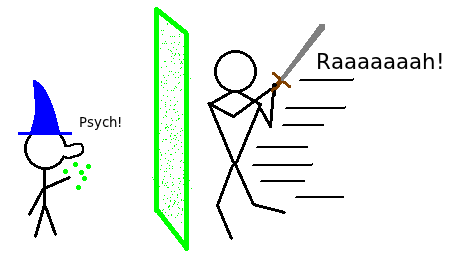
\includegraphics{Pics/WallOfForce.png}
\end{figure*}

\paragraph{Augment:} You can augment this spell in one or both of the following ways:
\begin{enumerate}
 \item For every additional spell point you spend, you get an additional 10-ft. square of wall.
 \item If you spend four additional spell points, the wall as a whole does not need to be flat, although each individual 10' section still has to be.
\end{enumerate}
\subsubsection{Wall of Ice}
\label{Spell:WallOfIce}
Evocation [Cold]
\\ \textbf{Level:} Sor/Wiz 4
\\ \textbf{Components:} V, S
\\ \textbf{Casting Time:} 1 standard action
\\ \textbf{Range:} Medium (100 ft. + 10 ft./level)
\\ \textbf{Effect:} Ice wall whose area consists of up to seven 5' squares (S)
\\ \textbf{Duration:} 1 min./level
\\ \textbf{Saving Throw:} See text
\\ \textbf{Spell Resistance:} No
\\ \textbf{Spell Points:} 7

\emph{You conjure a solid block of ice.}

This spell creates a wall of ice that merges into adjoining surfaces. 
A wall of ice is 1 inch thick per caster level and composed of up to seven 5-foot squares, 
which must join one another. 
You can double the wall's area by halving its thickness. 
The wall cannot be conjured so that it occupies the same space as a creature or another object.

You can create a wall of ice in almost any shape you desire. 
The wall created need not be vertical, nor rest upon any firm foundation; however, 
it must merge with and be solidly supported by existing stone. 
It can be used to bridge a chasm, for instance, or as a ramp. 
For this use, if the span is more than 20 feet, the wall must be arched and buttressed. 
This requirement reduces the spell's area by half. 
The wall can be crudely shaped to allow crenellations, 
battlements, and so forth by likewise reducing the area.

Walking along the vertical surface of a wall of ice requires a DC 10 balance check.
Climbing up a wall of ice follows normal rules for climbing, with a +5 modifier
to the DC for the surface being slippery.

Like any other solid wall, this one can be destroyed by a disintegrate spell or by normal means such as breaking and chipping. 
Each 5-foot square of wall has 3 hit points per inch of thickness. Its hardness is 0.
Creatures can hit the wall automatically. 
A section of wall whose hit points drop to 0 is breached. 
If a creature tries to break through the wall with raw strength rather than attacks, 
the DC for the Strength check is 22.

It is possible, but difficult, to trap mobile opponents within or under a wall of ice, 
provided the wall is shaped so it can hold the creatures. 
Creatures can avoid entrapment with successful Reflex saves.

The wall is crystal clear, and does not block line of sight (although
spot checks taken through the wall take a -2 penalty).
Noticing the wall is a DC 0 spot check.
The wall does block line of effect.

\paragraph{Augment:} For every additional spell point you spend, you get an additional 5' square of wall you can place, 
and the strength check DC required to burst through it increases by 1.
\subsubsection{Wall of Iron}
\label{Spell:WallOfIron}
Conjuration (Creation)
\\ \textbf{Level:} Conjurer 6
\\ \textbf{Components:} V, S
\\ \textbf{Casting Time:} 1 standard action
\\ \textbf{Range:} Medium (100 ft. + 10 ft./level)
\\ \textbf{Effect:} Iron wall whose area is up to eleven 5-ft. squares; see text
\\ \textbf{Duration:} 1 hour/level
\\ \textbf{Saving Throw:} None
\\ \textbf{Spell Resistance:} No
\\ \textbf{Spell Points:} 11

\emph{''Doesn't last long enough to be sold, I'm afraid.``}

You cause a flat, vertical iron wall to spring into being. 
The wall inserts itself into any surrounding nonliving material if its area is sufficient to do so,
keeping it in place. 
The wall cannot be conjured so that it occupies the same space as a creature or another object. 
It must always be a flat plane, though you can shape its edges to fit the available space.

A wall of iron is 1 inch thick per four caster levels. %You can double the wall's area by halving its thickness. 
Each 5-foot square of the wall has 30 hit points per inch of thickness and hardness 10. 
A section of wall whose hit points drop to 0 is breached. 
If a creature tries to break through the wall with a single attack, the DC for the Strength check is 25 + 2 per inch of thickness.

If you desire, the wall can be created (nearly) vertically resting on a flat surface but not attached to the surface, 
so that it tips over and crushes creatures caught in the area (the wall must have sufficient space to tip over). 
A wall so conjured crashes to the ground after one round (on your initiative in the next round) if left to fall on its own.
Any large or smaller creature caught under the wall (naturally, the effective area becomes equal to the size of the wall)
when it touches down takes 11d6 points of damage and is Immobilized until he makes a successful DC 40 strength or escape artist check 
(or the wall is dispelled or expires).
The presence of any huge or larger creature in the affected area causes the wall to automatically stabilize, negating the effect for all creatures.

In the round the wall spends falling, a creature adjacent to one of the squares in which the wall was conjured can use a move action 
to reverse the direction of the fall with a DC 30 strength check, 
or stabilize the wall in the position in which it was originally conjured with a DC 30 strength check and a DC 20 Balance check.

\paragraph{Augment:} For every additional spell point you spend, you can create a wall with an area of one additional 5' square. This increases the
damage dealt to crushed creatures by 1d6, and increases the DC of the strength or escape artist checks to escape after being pinned by the wall by 1, 
as well as the strength DCs to affect the fall of the wall.
\subsubsection{Wall of Stone}
\label{Spell:WallOfStone}
Conjuration (Creation) [Earth]
\\ \textbf{Level:} Earth 5, Sor/Wiz 5
\\ \textbf{Effect:} Stone wall whose area consists of up to nine 5' squares (S)
\\ \textbf{Duration:} Instantaneous
\\ \textbf{Spell Points:} 9

\textbf{A thick rock outcropping appears.}

This spell works like \nameref{Spell:WallOfIce}, except as noted here.

\begin{itemize}
 \item A wall of stone is 1 inch thick per two caster levels.
 \item No balance checks are required to remain stable on a stone wall, and climbers are not at a particular disadvantage.
 \item Each 5-foot square of stone wall has 15 hit points per inch of thickness. Its hardness is 8.
The DC for a Strength check to break through it is 30.
 \item Stone walls are opaque, and block line of sight.
\end{itemize}

\paragraph{Augment:} For every additional spell point you spend, you get an additional 5' square of wall you can place, 
and the strength check DC required to burst through it increases by 1.
\subsubsection{Wall of Thorns}
\label{Spell:WallOfThorns}
Conjuration (Creation)
\\ \textbf{Level:} Plant 5, Ranger 5
\\ \textbf{Components:} V, S
\\ \textbf{Casting Time:} 1 standard action
\\ \textbf{Range:} Medium (100 ft. + 10 ft./level)
\\ \textbf{Effect:} Wall of thorny brush, up to nine 10-ft. cubes(S)
\\ \textbf{Duration:} 10 min./level (D)
\\ \textbf{Saving Throw:} None
\\ \textbf{Spell Resistance:} No
\\ \textbf{Spell Points:} 9

\emph{You create a barrier of very tough, pliable, tangled brush bearing needle-sharp thorns as long as a human's finger.}

Any creature forced into or attempting to move through a wall of thorns takes slashing damage per round of movement equal to 25 minus the creature's AC (minimum 0). Dexterity and dodge bonuses to AC do not count for this calculation.

You can make the wall as thin as 5 feet thick, which allows you to shape the wall as a number of 10-by-10-by-5-foot blocks equal to twice your caster level. This has no effect on the damage dealt by the thorns, but any creature attempting to break through takes that much less time to force its way through the barrier.

Creatures can force their way slowly through the wall by making a Strength check as a full-round action. For every 5 points by which the check exceeds 20, a creature moves 5 feet (up to a maximum distance equal to its normal land speed). Of course, moving or attempting to move through the thorns incurs damage as described above. A creature trapped in the thorns can choose to remain motionless in order to avoid taking any more damage.

Any creature within the area of the spell when it is cast takes damage as if it had moved into the wall and is caught inside. In order to escape, it must attempt to push its way free, or it can wait until the spell ends. Creatures with the ability to pass through magically overgrown areas unhindered can pass through a wall of thorns at normal speed without taking damage.

A wall of thorns can be breached by slow work with edged weapons. Chopping away at the wall creates a safe passage 1 foot deep for every 10 minutes of work. Fire burns a 10' cube of it away in 10 minutes.

Despite its appearance, a wall of thorns is not actually a living plant, and thus is unaffected by spells that affect plants.

\paragraph{Augment:} For every additional spell point you spend, you can create a wall with an area of one additional 5' square, and the damage dealt by the spell increases by 1.

\subsubsection{Water Walk}
\label{Spell:WaterWalk}
Transmutation [Water]
\\ \textbf{Level:} Ranger 3, Water 3
\\ \textbf{Components:} V, S
\\ \textbf{Casting Time:} 1 standard action
\\ \textbf{Range:} Touch
\\ \textbf{Targets:} Up to five touched creatures
\\ \textbf{Duration:} 10 min./level (D)
\\ \textbf{Saving Throw:} Will negates (harmless)
\\ \textbf{Spell Resistance:} Yes (harmless)
\\ \textbf{Spell Points:} 5

\emph{''For a spell no more complicated than this, it sure freaks out the villagers.``}

The transmuted creatures can tread on any liquid as if it were firm ground. 
Mud, oil, snow, quicksand, running water, ice, and even lava can be traversed easily, since the subjects' feet hover an inch or two above the surface. 
(Creatures crossing molten lava still take damage from the heat because they are near it.) 
The subjects can walk, run, charge, or otherwise move across the surface as if it were normal ground.

If the spell is cast underwater (or while the subjects are partially or wholly submerged in whatever liquid they are in), the subjects are borne toward the surface at 60 feet per round until they can stand on it.

\paragraph{Augment:} For every additional spell point you spend, you can target an additional creature when casting this spell.
\subsubsection{Waves of Fatigue}
\label{Spell:WavesOfFatigue}
Necromancy
\\ \textbf{Level:} Sor/Wiz 5
\\ \textbf{Components:} V, S
\\ \textbf{Casting Time:} 1 standard action
\\ \textbf{Range:} 30 ft.
\\ \textbf{Area:} Cone-shaped burst
\\ \textbf{Duration:} Instantaneous
\\ \textbf{Saving Throw:} No
\\ \textbf{Spell Resistance:} Yes
\\ \textbf{Spell Points:} 9

\emph{Waves of negative energy radiate outwards from you.}

All living creatures in the spell's area are rendered \emph{fatigued}. This spell has no effect on a creature that is already \emph{fatigued}.

\paragraph{Augment:} If you spend an additional 4 spell points, this spell renders its victims \emph{exhausted} rather than \emph{fatigued}.
\subsubsection{Web}
\label{Spell:Web}
Conjuration (Creation)
\\ \textbf{Level:} Sor/Wiz 2, Vermin 2
\\ \textbf{Components:} V, S
\\ \textbf{Casting Time:} 1 standard action
\\ \textbf{Range:} Medium (100 ft. + 10 ft./level)
\\ \textbf{Effect:} Web between two anchors
\\ \textbf{Duration:} 10 min./level (D)
\\ \textbf{Saving Throw:} Reflex negates; see text
\\ \textbf{Spell Resistance:} No
\\ \textbf{Spell Points:} 3

\emph{You create a many-layered mass of strong, sticky strands, similar to spider webs but far larger and tougher.}

The web you create must be anchored to two or more solid and diametrically opposed points or else it collapses upon itself and disappears. 
The two anchor points must be within 40' of each other, making that the maximum length of the web. The web extends 15' down from the anchoring points. 

To determine the web's ground area, draw a line between the two anchors. The web occupies all squares crossed by that line.

%Creatures caught within a web become Immobilized among the gluey fibers. 
%Attacking a creature in a web won't cause you to become Immobilized.
Anyone in the effect's area when the spell is cast must make a Reflex save. 
If this save succeeds, the creature escapes, and is shunted to the nearest empty space 
(if multiple squares are equally valid, the creature chooses which square it ends up in). 
%This movement counts against the creature's movement on its next turn (or its 5' step), possibly restricting its actions.

If the save fails, the creature is \emph{immobilized} and can't move from its space,  
but can break loose by spending a full round action and making a DC 20 Strength check or a DC 25 Escape Artist check 
(if the creature attempting to escape succeeds by 4 or more, the square of webs the creature occupied is destroyed).
Once loose, the creature ends up in the nearest empty square, as if it had succeeded on the initial reflex save.

If you have web between you and an opponent, it provides cover.

The strands of a web spell are extremely flammable. 
A magic flaming sword can slash them away as easily as a hand brushes away cobwebs, automatically destroying a 
5'x5' square of the webs with a single attack.
Any fire can set the webs alight and burn away a square in 1 round. 
All creatures Immobilized within a square of flaming webs take 2d4 points of fire damage from the flames.

Each square of webs has 20 hit points and hardness 5 (slashing weapons ignore this hardness).
Each square can be burst with a DC 24 Strength check.

%Web can be made permanent with a permanency spell. A permanent web that is damaged (but not destroyed) regrows in 10 minutes.

%\paragraph{Augment:} For every 2 additional spell points you spend, this spell's save DC increases by 1.

\subsubsection{Web Strand}
\label{Spell:WebStrand}
Conjuration (Creation)
\\ \textbf{Level:} Vermin 1
\\ \textbf{Components:} V, S
\\ \textbf{Casting Time:} 1 standard action
\\ \textbf{Range:} Close (25 ft. + 5 ft./2 levels)
\\ \textbf{Target:} One Medium or smaller creature
\\ \textbf{Duration:} 5 rounds
\\ \textbf{Saving Throw:} None
\\ \textbf{Spell Resistance:} No
\\ \textbf{Spell Points:} 1

\emph{You conjure forth a sticky strand of webbing, like that of an oversized spider, and hurl it at your enemy.}

You throw the strand of webbing as a ranged touch attack at any creature in range. 
On a successful hit, the subject is covered in goo and becomes \emph{entangled}. 
The goo evaporates at the end of the spell's duration.

\paragraph{Augment:} For every 2 additional spell points you spend, this spell can affect a target one size category larger.

\subsubsection{Whirlwind}
\label{Spell:Whirlwind}
Evocation [Air]
\\ \textbf{Level:} Air 8
\\ \textbf{Components:} V, S
\\ \textbf{Casting Time:} 1 standard action
\\ \textbf{Range:} Long (400 ft. + 40 ft./level)
\\ \textbf{Effect:} Cyclone 10 ft. wide at base, 30 ft. wide at top, and 30 ft. tall
\\ \textbf{Duration:} 1 round/level (D)
\\ \textbf{Saving Throw:} Reflex negates; see text
\\ \textbf{Spell Resistance:} No
\\ \textbf{Spell Points:} 15

\emph{This spell creates a powerful cyclone of raging wind.} 

The cyclone can move through the air, along the ground, or over water at a speed of 60 feet per round. 

You can concentrate on controlling the cyclone's every movement or specify a simple program. 
Directing the cyclone's movement or changing its programmed movement is a standard action for you. 
The cyclone always moves during your turn. 
If the cyclone exceeds the spell's range, it moves in a random, uncontrolled fashion for 1d3 rounds and then dissipates. (You can't regain control of the cyclone, even if comes back within range.)

Any large or smaller creature that comes in contact with the spell effect must succeed on a Reflex save or take 7d6 points of damage. 
Regardless of the outcome of the first save, a medium or smaller creature must succeed on a second one or be picked up bodily by the cyclone and held suspended in its powerful winds, taking 2d8 points of damage each round on your turn with no save allowed. This is considered continuous damage for purposes of determining whether or not concentration checks are needed to use abilities. Escaping the cyclone via mundane means (even flight) requires a DC 40 escape artist check. A creature who escapes is \emph{blown away} in a direction of its choosing, away from the cyclone.

You may direct the cyclone to eject any carried creatures whenever you wish. When so released, they are \emph{blown away} in a direction of your choosing, away from the cyclone.

\paragraph{Augment:} For every additional spell point you spend, the spell's initial damage increases by one die (d6), and the escape artist DC to get out of the cyclone increases by 1.
\subsubsection{Widowmaker Blade}
\label{Spell:WidowmakerBlade}
Necromancy [Death, Evil]
\\ \textbf{Level:} Blackguard 5
\\ \textbf{Components:} V, S
\\ \textbf{Casting Time:} 1 standard action
\\ \textbf{Range:} Touch
\\ \textbf{Targets:} One melee weapon
\\ \textbf{Duration:} 1 round/level
\\ \textbf{Saving Throw:} Will negates (harmless, object); fortitude negates; see text
\\ \textbf{Spell Resistance:} Yes (harmless, object); no; see text
\\ \textbf{Spell Points:} 9

\emph{The weapon you touch becomes an instrument to cull the weak from the battlefield.} 

Any living creature with HD equal to or less than 7 must succeed on a Fortitude save or die if struck in combat with this weapon. 
Spell resistance does not apply against the death effect.

In addition, the wielder gains the benefit of the Cleave feat as long as he holds the weapon. If he already has the Cleave feat, he gains the Great Cleave feat instead. If he already has the Great Cleave feat, he receives no additional benefit.

\paragraph{Augment:} For every additional spell point you spend, the weapon can affect a creature with 1 more HD.

\subsubsection{Wind Wall}
\label{Spell:WindWall}
Evocation [Air]
\\ \textbf{Level:} Air 3, Ranger 2, Sor/Wiz 3
\\ \textbf{Components:} V, S
\\ \textbf{Casting Time:} 1 standard action
\\ \textbf{Range:} Medium (100 ft. + 10 ft./level)
\\ \textbf{Effect:} Wall up to 10 ft./level long and 5 ft./level high (S)
\\ \textbf{Duration:} 1 round/level
\\ \textbf{Saving Throw:} Special; see text
\\ \textbf{Spell Resistance:} Yes
\\ \textbf{Spell Points:} Air 5, Ranger 3, Sor/Wiz 3

\emph{You create an area infested with gusts of powerful wind directed downwards, hindering the advance of creatures and making ranged attacks very difficult.}

The wall you create is 5 feet thick, and not directly visible. However, dirt and loose
debris in its area is blown around, often giving it away. While the wall must be vertical, 
you can shape it in any continuous path along the ground that you like. 
It is possible to create cylindrical or square wind walls to enclose specific points.

Any physical missiles (arrows, crossbow bolts, javelins, magically propelled stones, and so on) whose line of effect passes through the
wind wall have a 50\% miss chance.

Passing through the wall is difficult.
Every time a creature enters a space the wall occupies, it must make a strength check or be knocked down.
The DC for the strength check is equal to the spell's save DC. 
For every size category the creature is above medium, it gains a +4 bonus on the strength check.
For every size category the creature is below medium, it suffers a -4 penalty on the strength check.
Flying creatures or those for some other reason not in contact with the ground (such as due to jumping) 
suffer a -8 penalty on the strength check in addition to the modifiers for size, above.

If the creature succeeds on the strength check, it manages to push through the wall unhindered.
If the creature fails, it is knocked prone in the space it was trying to enter, and takes 1d6 points of nonlethal damage.
Flying creatures are instantly knocked to the ground, and take damage as if they had fallen from the distance they were
flying (\nameref{Spell:ControlFall} does not prevent this).

Standing up while in the wind wall's area is difficult, and requires a successful strength check (which uses the same modifiers
and DCs as those for entering a square filled by the wall).

It is impossible to charge through a wind wall.
Gases, most gaseous breath weapons, and creatures in \nameref{Spell:GaseousForm} cannot pass through the wall.
It is no barrier to incorporeal creatures and air elementals.

The force of the gust automatically extinguishes candles, torches, and similar unprotected flames in its area. 
It causes protected flames, such as those of lanterns, to dance wildly and has a 50\% chance to extinguish those lights.

% \paragraph{Augment:} For every 2 additional spell points you spend, this spell's save DC increases by 1, and the miss chance
% suffered by missiles passing through the wall is increased by 10\% (to a maximum of 100\%).
\paragraph{Augment:} For every additional spell point you spend, the miss chance suffered by missiles passing though the wall
is increased by 5\% (to a maximum of 100\%).
\subsubsection{Wish}
\label{Spell:Wish}
Evocation
\\ \textbf{Level:} Sor/Wiz 9
\\ \textbf{Components:} V
\\ \textbf{Casting Time:} 1 standard action
\\ \textbf{Range:} See text
\\ \textbf{Target, Effect, or Area:} See text
\\ \textbf{Duration:} See text
\\ \textbf{Saving Throw:} See text
\\ \textbf{Spell Resistance:} Yes
\\ \textbf{Spell Points:} 17, XP

\emph{Wish is the mightiest spell a spellcaster can cast. By simply speaking aloud, you can alter reality to better suit you.
It is a tool fit for a god.}

\begin{figure*}
  \caption{Sorcerer receives the world's largest cockerel as a result of his Wish.}
  \centering
    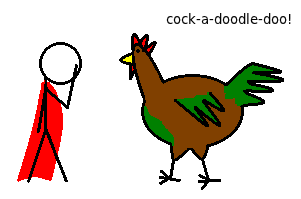
\includegraphics{Pics/Wish.png}
\end{figure*}

A Wish can produce any one of the following effects. 
These effects are easily within the power of the Wish, unintended consequences are next to impossible.
\begin{itemize}
  \item Duplicate any wizard spell of 8th level or lower, other than a spell restricted to specialists of schools other than your own.
  \item Duplicate any wizard spell of 7th level or lower, even if it is a spell restricted to specialists of schools other than your own.
  \item Duplicate any other spell of 6th level or lower.
  \item Undo the harmful effects of many other spells, such as \nameref{Spell:GeasQuest} or an augmented \nameref{Spell:Confusion}.
  \item Create a nonmagical item of up to 25,000 gp in value.
  \item Create a magic item, or add to the powers of an existing magic item (see XP cost below).
  %\item Grant a creature a +1 inherent bonus to an ability score. Two to five Wish spells cast in succession (which need not be an immediate succession) can grant a creature a +2 to +5 inherent bonus to an ability score (two Wishes for a +2 inherent bonus, three for a +3 inherent bonus, and so on).
  \item Grant a creature a +1 inherent bonus to an ability score, or increase an existing inherent bonus to an ability score by one.
  Inherent bonuses are instantaneous, so they cannot be dispelled. An inherent bonus may not exceed +5 for a single ability score.
  %An inherent bonus may not exceed +5 for a single ability score, and inherent bonuses to a particular ability score do not stack, so only the best one applies.
  \item Remove injuries and afflictions. A single Wish can aid one creature per caster level, and all subjects are cured of the same kind of affliction. 
  For example, you could heal all the damage you and your companions have taken, or remove all poison effects from everyone in the party, but not do both with the same Wish. 
  A Wish can never restore the experience point loss from casting a spell or the level or Constitution loss from being raised from the dead.
  \item Revive the dead. A Wish can bring a dead creature back to life by duplicating a resurrection spell. .
  A Wish can revive a dead creature whose body has been destroyed, but the task takes two Wishes, one to recreate the body and another to infuse the body with life again. 
  A Wish cannot prevent a character who was brought back to life from losing an experience level.
  \item Transport travelers. A Wish can lift one creature per caster level from anywhere on any plane and place those creatures anywhere else on any plane regardless of local conditions, 
  excepting the direct intervention of a deity. 
  An unwilling target gets a Will save to negate the effect, and spell resistance (if any) applies.
  \item Undo misfortune. A Wish can undo a single recent event. 
  The Wish forces a reroll of any roll made within the last round (including your last turn). 
  Reality reshapes itself to accommodate the new result. 
  For example, a Wish could undo an opponent's successful save, a foe's successful critical hit (either the attack roll or the critical roll), 
  a friend's failed save, and so on. The reroll, however, may be as bad as or worse than the original roll. 
  An unwilling target gets a Will save to negate the effect, and spell resistance (if any) applies.
  \item Produce any other effect whose power level is in line with the above effects
\end{itemize}
You may try to use a Wish to produce greater effects than these, but doing so is dangerous. 
(The Wish may pervert your intent into a literal but undesirable fulfillment or only a partial fulfillment.)
You can describe virtually any effect, but you must do so in 10 words or less.

Duplicated spells allow saves and spell resistance as normal (but save DCs are for the number of spell points spent on the Wish).

\emph{Experience Cost:} The minimum XP cost for casting Wish is 5,000 XP. 
When a Wish duplicates a spell that has an XP cost, you must pay 5,000 XP or that cost, whichever is more. 
When a Wish creates or improves a magic item, you must pay twice the normal XP cost for crafting or improving the item, plus an additional 5,000 XP. 

\subsubsection[Limited Wish]{Wish, Limited}
\label{Spell:LimitedWish}
Evocation
\\ \textbf{Level:} Magic 7, Sor/Wiz 7
\\ \textbf{Components:} V
\\ \textbf{Casting Time:} 1 standard action
\\ \textbf{Range:} See text
\\ \textbf{Target, Effect, or Area:} See text
\\ \textbf{Duration:} See text
\\ \textbf{Saving Throw:} See text
\\ \textbf{Spell Resistance:} Yes
\\ \textbf{Spell Points:} 13, XP

\emph{You learn to create nearly any type of effect.}

A Limited Wish can do any of the following:
\begin{itemize}
\item Duplicate any wizard spell of 6th level or lower, other than a spell restricted to specialists of schools other than your own.
\item Duplicate any wizard spell of 5th level or lower,  even if it is a spell restricted to specialists of schools other than your own.
\item Duplicate any other spell of 4th level or lower.
\item Undo the harmful effects of many spells, such as \nameref{Spell:GeasQuest} or an augmented \nameref{Spell:Confusion}.
\item Produce any other effect whose power level is in line with the above effects, 
such as a single creature automatically hitting on its next attack or taking a -7 penalty on its next saving throw.
\end{itemize}
A duplicated spell allows saving throws and spell resistance as normal (but save DCs are for the number of spell points spent on the Wish).

When Limited Wish duplicates a spell that has an XP cost, you must pay that cost or 300 XP, whichever is more. 

\emph{Experience cost:} 300 XP or more (see above).
\subsubsection{Wombat's Boost}
\label{Spell:WombatsBoost}
Transmutation
\\ \textbf{Level:} Assassin 2, Blackguard 2, Cleric 2, Paladin 2, Sor/Wiz 2
\\ \textbf{Components:} V, S
\\ \textbf{Casting Time:} 1 standard action
\\ \textbf{Range:} Touch
\\ \textbf{Target:} Creature touched; see text
\\ \textbf{Duration:} 1 min./level
\\ \textbf{Saving Throw:} Will negates (harmless)
\\ \textbf{Spell Resistance:} Yes
\\ \textbf{Spell Points:} 3

\emph{The affected creature is infused with power.} 

The creature is granted a +4 enhancement bonus to a single ability score of the caster's choice, chosen at the time of casting. 

The individual functions of this spell are often named after animals that embody the ability in question in the
eyes of some scolars. They are \emph{Bull's Strength}, \emph{Cat's Grace} (Dexterity),
\emph{Bear's Endurance} (Constitution), \emph{Owl's Wisdom}, 
\emph{Fox's Cunning} (Intelligence), and \emph{Eagle's Splendor} (Charisma).

Unlike \nameref{Spell:AlterSelf}, the enhancement to your ability does not result in a physical change -
the improvement is due to a direct magical infusion.

\begin{figure*}
  \caption{Wizard casts Bull's Strength on himself to know how it is to be as strong as the Fighter.}
  \centering
    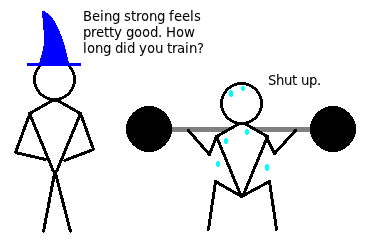
\includegraphics{Pics/Wombat.png}
\end{figure*}

\paragraph{Augment:} You can Augment this spell in one or both of the following ways:
\begin{enumerate}
 \item If you spend two additional spell points, the spell's range increases to Close.
 \item For every two additional spell points you spend, the spell can affect an additional target.
\end{enumerate}
\subsubsection{Word of God}
\label{Spell:WordOfGod}
Evocation [Sonic, see text]
\\ \textbf{Level:} Blackguard 6, Chaos 7, Evil 7, Good 7, Law 7, Paladin 6
\\ \textbf{Components:} V
\\ \textbf{Casting Time:} 1 standard action
\\ \textbf{Range:} 40 ft.
\\ \textbf{Area:} Creatures in a 40-ft.-radius spread centered on you
\\ \textbf{Duration:} Instantaneous; see text
\\ \textbf{Saving Throw:} None or Will negates; see text
\\ \textbf{Spell Resistance:} Yes
\\ \textbf{Spell Points:} Chaos 13, Evil 13, Good 13, Law 13, Paladin 11

\emph{A single bass note of incredible power suffuses the area.}

When casting this spell, choose an alignment. The spell gains that alignment as a descriptor.

Any creature not of your selected alignment within the spell's area suffers the ill effects
described on the \nameref{tab:WordOfGod} table. This includes you, if you are not of the selected alignment.
\begin{table*}
\label{tab:WordOfGod}
\caption{Word of God}
\makebox[\textwidth]{
\begin{tabular}{lccccl}
\toprule
&\multicolumn{4}{c}{Alignment selected}&\\ \cmidrule(r){2-5}
$\leq$HD&Chaotic&Evil&Good&Law&Duration\\
&(Word of Chaos)&(Blasphemy)&(Holy Word)&(Dictum)&\\
\midrule
14&Unaffected&Unaffected&Unaffected&Unaffected&N/A\\
13&Deafened&Deafened&Deafened&Deafened&Permanent\\
9-12&Stunned (1d3)&Blinded (2d4)&Nauseated (1d4)&Dazed (1d3)&Rounds, see entry\\
4-8&Paralyzed&Paralyzed&Paralyzed&Paralyzed&1d10 minutes\\
3&Killed&Killed&Killed&Killed&Instantaneous\\
\bottomrule
\end{tabular}}
\end{table*}

\begin{figure*}
  \caption{Cleric uses Word of God effectively.}
  \centering
    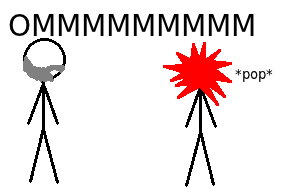
\includegraphics{Pics/WordOfGod.png}
\end{figure*}

The number of HD indicated on the table refers to the maximum number of HD a creature may have in order to be subjected to the corresponding effect.
The effects are cumulative and concurrent.
For example, an evil creature with 10 HD caught in a good-aligned Word of God is \emph{nauseated} and \emph{deafened}.

\paragraph{Augment:} For every additional spell point you spend, the number of HD indicated in each row of the first column of the \nameref{tab:WordOfGod} table increases by 1.
\subsubsection{Word of Recall}
\label{Spell:WordOfRecall}
Conjuration (Teleportation)
\\ \textbf{Level:} Protection 6, Travel 6
\\ \textbf{Components:} V
\\ \textbf{Casting Time:} 1 standard action
\\ \textbf{Range:} Unlimited
\\ \textbf{Target:} You and touched objects or other willing creatures
\\ \textbf{Duration:} Instantaneous
\\ \textbf{Saving Throw:} None or Will negates (harmless, object)
\\ \textbf{Spell Resistance:} No or Yes (harmless, object)
\\ \textbf{Spell Points:} 11

\emph{''HOME! ``}

Word of recall teleports you instantly back to your sanctuary when cast. 

You must designate this sanctuary before using the spell.
Doing so involves a simple ritual performed at the site, taking one hour. 
The sanctuary must be a place very familiar to you. 
The actual point of arrival is a designated area no larger than 10 feet by 10 feet.
You can choose a new sanctuary by re-doing the ritual at another site.

You can be transported any distance within a plane but cannot travel between planes. 
You can transport, in addition to yourself, any objects you carry, as long as their weight doesn't exceed your maximum load. 
You may also bring one additional willing creature (carrying gear or objects up to its maximum load) per three caster levels. 
All creatures to be transported must be in contact with one another, and at least one of those creatures must be in contact with you. Exceeding this limit causes the spell to fail.

An unwilling creature can't be teleported by word of recall. Likewise, a creature's Will save (or spell resistance) prevents items in its possession from being teleported. Unattended, nonmagical objects receive no saving throw.

\paragraph{Augment:} If you spend 4 additional spell points, the spell can teleport you towards a sanctuary on another plane.


\subsection{'Z' Spells}
\subsubsection{Zone of Truth}
\label{Spell:ZoneOfTruth}
Abjuration
\\ \textbf{Level:} Law 2, Paladin 2
\\ \textbf{Components:} V, S
\\ \textbf{Casting Time:} 1 standard action
\\ \textbf{Range:} Close (25 ft. + 5 ft./2 levels)
\\ \textbf{Area:} 10-ft.-radius emanation centered on a point in space
\\ \textbf{Duration:} 10 min./level (D)
\\ \textbf{Saving Throw:} None
\\ \textbf{Spell Resistance:} No
\\ \textbf{Spell Points:} 3
% \Level{Law 2, Paladin 2}
% \Components{V, S}
% \CastingTime{1 standard action}
% \Range{\CloseRange}
% \Area{10-ft.-radius emanation centered on a point in space}
% \Duration{\TenMinLevelDuration{\DismissibleSpell}}
% \SavingThrow{None}
% \SRno
% \SP{3}

\emph{Your tongue physically resists when you try speaking anything but the honest truth.}

All creatures within the spell's area take a penalty on Bluff checks equal to 10 + your caster level.

\paragraph{Augment:} If you spend 4 additional spell points, the spell's duration changes to 1 day.

\newpage
\subsection{Where's my favorite spell?}
\label{sec:MissingSpells}
This conversion does not contain all the spells in the \href{http://www.wizards.com/default.asp?x=d20/article/srd35}{d20 srd}.
Some were merged into others, some were merely renamed, but some truly aren't here. 
The most common reason for a spell not being included was it being too limited in scope to justify being a spell of its own under the revised system.
This is a list of all SRD spells that do not have a converted spell with the same name.
Note that some spells might have changed levels.
{\small
\begin{itemize}
 \item Acid Fog: Merged into Deadly Fog.
 \item Acid Splash: See the Cantrips class feature.
 \item Analyze Dweomer: Merged into Identify.
 \item Animal Growth: Merged into Alter Animal's Size.
 \item Animal Shapes: Removed. Replace with Form of the Predator for item creation and other purposes.
 \item Animal Trance: Removed. Replace with Pattern for item creation and other purposes.
 \item Antipathy: Merged into Telepathic Beacon
 \item Antiplant Shell: Removed. Replace with Antilife Shell for item creation and other purposes.
 \item Arcane Lock: Merged into Open/Close.
 \item Arcane Mark: See the Cantrips class feature.
 \item Arcane Sight, Greater: Merged into Detect Magic.
 \item Arcane Sight: Merged into Detect Magic.
 \item Banishment: Merged into Dismissal.
 \item Bear's Endurance, Bull's Strength, Cat's Grace, Eagle's Splendor, Fox's Cunning and Owl's Wisdom, Mass: Merged into Wombat's Boost.
 \item Bear's Endurance, Bull's Strength, Cat's Grace, Eagle's Splendor, Fox's Cunning and Owl's Wisdom: Merged into Wombat's Boost.
 \item Blasphemy/Dictum/Holy Word/Word of Chaos: Merged into Word of God.
 \item Break Enchantment: Merged into Remove Curse.
 \item Burning Hands: Merged into Energized Touch.
 \item Call Lightning Storm: Merged into Call Lightning.
 \item Calm Animals: Removed. Replace with Calm Emotions for item creation and other purposes.
 \item Cause Fear: Renamed Fear.
 \item Changestaff: Merged into Liveoak.
 \item Charm Animal: Isn't this what Wild Empathy is for? Removed. Replace with Charm for item creation and other purposes.
 \item Charm Monster, Mass: Merged into Charm.
 \item Charm Monster: Merged into Charm.
 \item Charm Person: Renamed Charm.
 \item Chill Touch: Merged into Energized Touch.
 \item Circle of Death: Merged into Life and Death.
 \item Clenched Fist: Pending. Can't think of more Hand spells.
 \item Clone: Merged into Gentle Repose.
 \item Cloudkill: Merged into Noxious Vapors.
 \item Command Plants: Renamed Command Nature's Allies.
 \item Continual Flame: Merged into Light.
 \item Control Plants: Renamed Control Nature's Allies.
 \item Create Greater Undead: Merged into Create Undead.
 \item Create Water: See Water domain.
 \item Crushing Hand: Pending. Can't think of more Hand spells.
 \item Cure Critical Wounds, Mass: Merged into Cure Wounds.
 \item Cure Critical Wounds: Merged into Cure Wounds.
 \item Cure Light Wounds, Mass: Merged into Cure Wounds.
 \item Cure Light Wounds: Merged into Cure Wounds.
 \item Cure Moderate Wounds, Mass: Merged into Cure Wounds.
 \item Cure Moderate Wounds: Merged into Cure Wounds.
 \item Cure Serious Wounds, Mass: Merged into Cure Wounds.
 \item Dancing Lights: See the Cantrips class feature.
 \item Daylight: Merged into Light.
 \item Daze Monster: Merged into Daze.
 \item Deathwatch: Turned into a Healing domain ability.
 \item Deep Slumber: Merged into Sleep.
 \item Delayed Blast Fireball: Changed into a Metamagic feat. Replace with fireball for item creation and other purposes.
 \item Delay Poison: Merged into Antipoison.
 \item Demand: Removed, replaced with Scrying + the Scry and Die feat. Replace with Suggestion for item creation and other purposes.
 \item Destruction: Merged into Slay Living.
 \item Detect Animals or Plants: Removed. What is this even? Replace with 4 ranks in Spot for item creation and other purposes.
 \item Detect Chaos/Evil/Good/Law: Merged into Discern Alignment.
 \item Detect Snares and Pits: Removed. Replace with Trapfinding for item creation and other purposes.
 \item Detect Thoughts: Renamed Read Thoughts.
 \item Detect Undead: Removed. Replace with Discern Alignment
 \item Diminish Plants: Merged into Plant Growth.
 \item Discern Lies: Removed due to overlap with Zone of Truth.
 \item Discern Location: Renamed Absolute Revelation, due to me thinking that ``Discern Location'' and ``Location'' are too similar.
 \item Dispel Chaos/Evil/Good/Law: Merged into Dispel Alignment
 \item Dispel Magic, Greater: Merged into Dispel Magic.
 \item Displacement: Merged into Blur.
 \item Disrupt Undead: Removed. Replace with Align Water for item creation and other purposes.
 \item Divination: Merged into Augury.
 \item Dominate Animal: Merged into Dominate.
 \item Dominate Monster: Merged into Dominate.
 \item Dominate Person: Merged into Dominate.
 \item Doom: Merged into Fear.
 \item Energy Drain: Merged into Enervation.
 \item Enlarge Person, Mass: Merged into Alter Size.
 \item Enlarge Person: Merged into Alter Size.
 \item Erase: Removed. Replace with the Cantrip class feature for item creation and other purposes.
 \item Etherealness: Merged into Ethereal Jaunt.
 \item Fabricate: Merged into Mold Material.
 \item Feather Fall: Merged into Control Fall.
 \item Find the Path: Removed, pending inspiration. Replace with Legend Lore for purposes of item creation.
 \item Find Traps: Renamed Trap Intuition.
 \item Fire Shield: Renamed Aura of Fire.
 \item Fire Trap: Replaced with Explosive Runes.
 \item Flame Arrow: Renamed Energy Arrow.
 \item Flare: Merged into Light.
 \item Flesh to Stone: Merged into Transmute Flesh and Stone
 \item Fog Cloud: Merged into Fog.
 \item Forcecage: Merged into Resilient Sphere.
 \item Forceful Hand: Pending. Can't think of more Hand spells. Replace with one of the other ''hand`` spells for item creation and other purposes.
 \item Ghost Sound: Removed. Replace with Ventriloquism for item creation and other purposes.
 \item Glyph of Warding, Greater: Merged into Glyph of Warding.
 \item Good Hope: Removed due to redundancy.
 \item Grasping Hand: Pending. Can't think of more Hand spells.
 \item Guards and Wards: Changed into a magic item.
 \item Guidance: Removed. Replace with Bless for item creation and other purposes.
 \item Hallow/Unhallow: Partially removed, rest merged into Consecrate/Desecrate.
 \item Heal, Mass: Merged into Heal.
 \item Heroism, Greater: Merged into Heroism.
 \item Hide from Animals: Renamed Shroud the Weak Mind.
 \item Hide from Undead: Changed into a Death Domain granted power. Use Invisibility for its other function.
 \item Hold Monster, Mass: Merged into Hold Person.
 \item Hold Monster: Merged into Hold Person.
 \item Hold Person, Mass: Merged into Hold Person.
 \item Hold Portal: Merged into Open/Close.
 \item Holy Sword: Renamed Aligned Sword.
 \item Hypnotic Pattern: Merged into Pattern.
 \item Hypnotism: Merged into Pattern.
 \item Illusory Script: Pending inspiration.
 \item Illusory Wall: Replaced with Image. 
 \item Incendiary Cloud: Merged into Deadly Fog.
 \item Inflict Light, Moderate, Serious, and Critical Wounds, Mass: Merged into Inflict Wounds.
 \item Inflict Light, Moderate, Serious, and Critical Wounds: Merged into Inflict Wounds.
 \item Inflict minor wounds: Removed. Replace with Inflict Wounds for item creation and other purposes.
 \item Insanity: Merged into Confusion.
 \item Invisibility Sphere: Merged into Invisibility.
 \item Invisibility, Greater: Merged into Invisibility.
 \item Invisibility, Mass: Merged into Invisibility.
 \item Iron Body: Renamed Form of the Iron Golem.
 \item Ironwood: Merged into Transmute Metal and Wood.
 \item Jump: Merged into Control Fall.
 \item Knock: Merged into Open/Close.
 \item Know Direction: Make a DC 15 Survival check instead.
 \item Lesser Confusion: Renamed Random Action.
 \item Locate Creature: Merged into Locate.
 \item Locate Object: Merged into Locate.
 \item Longstrider: Travel domain granted ability.
 \item Lullaby: Is now a Bard class feature.
 \item Mage Hand: See the Cantrips class feature.
 \item Mage's Faithful Hound: Removed. replace with Summon Monster for item creation and other purposes.
 \item Mage's Lucubration: Not appropriate under this ruleset. Replace with Mnemonic Enhancer for item creation and other purposes.
 \item Magic Circle against Chaos/Evil/Good/Law: Merged into Aligned Protection.
 \item Magic Fang, Greater: Merged into Magic Weapon.
 \item Magic Fang: Merged into Magic Weapon.
 \item Magic Jar: Renamed Possession.
 \item Magic Mouth: Merged into Ventriloquism.
 \item Magic Weapon, Greater: Merged into Magic Weapon.
 \item Major Creation: Merged into Matter Creation.
 \item Major Image: Merged into Image.
 \item Mending: Merged into Repair.
 \item Message: Merged into Mental Link.
 \item Minor Creation: Renamed Matter Creation.
 \item Minor Image: Merged into Image.
 \item Mirage Arcana: Merged into Hallucinatory Terrain.
 \item Misdirection: Effectively merged into Magic Aura.
 \item Move Earth: To be put on the Earth domain list.
 \item Neutralize Poison: Merged into Antipoison.
 \item Nightmare: Merged into Dream.
 \item Obscure Object: Merged into Nondetection.
 \item Obscuring Mist: Renamed Fog.
 \item Overland Flight: Merged into Fly.
 \item Owl's Wisdom, Mass: Merged into Wombat's Boost.
 \item Pass without Trace: Now a Trickery domain granted power.
 \item Passwall: Removed. Replace with Mold Material for item creation and other purposes.
 \item Permanency: Removed due to changed design.
 \item Permanent Image: Merged into Image.
 \item Persistent Image: Merged into Image.
 \item Phantom Steed: Merged into Mount.
 \item Planar Binding, Greater: Merged into Planar Binding.
 \item Polymorph Any Object: Removed. Replace with Shapechange for item creation and other purposes.
 \item Power Word Kill: Merged into Power Word.
 \item Power Word Stun: Merged into Power Word.
 \item Prayer: Merged into Bless.
 \item Prestidigitation: See the Cantrips class feature.
 \item Prestidigitation: See the Cantrips class feature.
 \item Project Image: Pending inspiration.
 \item Protection from Chaos/Evil/Good/Law: Merged into Aligned Protection.
 \item Protection from Energy: Removed. Replace with Resist Energy for item creation and other purposes.
 \item Protection from Spells: Removed. Replace with Resistance for item creation and other purposes.
 \item Prying Eyes, Greater: Made redundant due to special senses now working through the eyes. Replace with Prying Eyes or True Seeing for item creation and other purposes.
 \item Quench: Removed for reasons of being too damn specific. Replace with Create Water (Water Domain ability) for item creation and other purposes.
 \item Rainbow Pattern: Merged into Pattern.
 \item Ray of Exhaustion: Merged into Touch of Fatigue
 \item Ray of Frost: See the Cantrips class feature.
 \item Read Magic: See the Cantrips class feature.
 \item Reduce Animal: Merged into Alter Animal's Size.
 \item Reduce Person, Mass: Merged into Alter Size.
 \item Reduce Person: Merged into Alter Size.
 \item Repulsion: Replaced With Antilife Shell.
 \item Rope Trick: Removed. Replace with Tiny Hut for item creation and other purposes.
 \item Scare: Merged into Fear.
 \item Scrying, Greater: Merged into Scrying.
 \item Secret Chest: Changed into a magic item.
 \item Secret Page: Pending inspiration.
 \item Secure Shelter: Merged into Tiny Hut.
 \item Seeming: Merged into Disguise.
 \item Shades: Merged into Shadow Conjuration
 \item Shadow Conjuration, Greater: Merged into Shadow Conjuration.
 \item Shadow Evocation, Greater: Merged into Shadow Evocation.
 \item Shambler: Removed. Replace with Summon Monster for item creation and other purposes.
 \item Shocking Grasp: Merged into Energized Touch.
 \item Shout, Greater: Merged into Shout.
 \item Silent Image: Renamed Image.
 \item Snare: Merged into Animate Rope.
 \item Solid Fog: Merged into Fog.
 \item Speak with Animals: Merged into Converse with Nature
 \item Speak with Plants: Merged into Converse with Nature.
 \item Speak with Plants: Merged into Converse with Nature.
 \item Spellstaff: Removed. Replace with Shillelagh for item creation and other purposes.
 \item Spider Climb: Merged into Animal's Movement.
 \item Statue: Removed on account of me not being able to figure out how to make this stuff ever worth a spell known.
 \item Status: Renamed Life Link.
 \item Stinking Cloud: Renamed Noxious Vapors.
 \item Stone Shape: Merged into Mold Material.
 \item Stone Tell: Merged into Converse with Nature.
 \item Stone to Flesh: Merged into Transmute Flesh and Stone
 \item Suggestion, Mass: Merged into Suggestion.
 \item Summon Monster I-IX: Merged into Summon Monster.
 \item Summon Nature's Ally I-IX: Merged into Summon Monster.
 \item Sunbeam: Merged into Sunburst.
 \item Symbol of Death: Changed into a magic item.
 \item Symbol of Fear: Changed into a magic item.
 \item Symbol of Insanity: Changed into a magic item.
 \item Symbol of Pain: Now a magic item.
 \item Symbol of Persuasion: Changed into a magic item.
 \item Symbol of Sleep: Now a magic item.
 \item Symbol of Stunning: Changed into a magic item.
 \item Symbol of Weakness: Changed into a magic item.
 \item Sympathy: Merged into Telepathic Beacon.
 \item Telekinetic Sphere: Merged into Resilient Sphere.
 \item Telepathic Bond: Merged into Mental Link.
 \item Teleport Object: Merged into Teleport.
 \item Teleport, Greater: Merged into Teleport.
 \item Tongues: Merged into Comprehend Languages.
 \item Transmute Metal to Wood: Renamed Transmute Metal and Wood
 \item Transmute Mud to Rock: Merged into Transmute Rock and Mud.
 \item Transmute Rock to Mud: Merged into Transmute Rock and Mud.
 \item Trap the Soul: Removed. Replace with Soul Bind for item creation and other purposes.
 \item Tree Shape: Renamed Form of the Plant.
 \item Tree stride: Removed due to extreme similarities with Transport via Plants. Replace with Transport via Plants for purposes of item creation.
 \item Undeath to Death:Merged into Life and Death.
 \item Undetectable Alignment: Renamed Mask Alignment.
 \item Veil: Merged into Disguise.
 \item Vision: Merged into Legend Lore
 \item Warp Wood: Removed. Replace with Shatter for item creation and other purposes.
 \item Water Breathing: Merged into Animal's Movement.
 \item Waves of Exhaustion: Merged into Waves of Fatigue.
 \item Weird: Merged into Phantasmal Killer.
 \item Whispering Wind: Merged into Sending.
 \item Wood Shape: Merged into Mold Material.
 \item Zone of Silence: Merged into Silence.
\end{itemize}
}

